\documentclass[a5paper,10pt]{book}

% ----------------- Packages ------------------
\usepackage[
  paper=a5paper,
  top=19mm,
  bottom=18mm,
  inner=23mm,
  outer=19mm,
  headheight=14pt,
  footskip=9mm
]{geometry}
\usepackage[utf8]{inputenc}
\usepackage[T1]{fontenc}
\usepackage{lmodern}
\usepackage{setspace}
\usepackage{amsmath, amssymb}
\usepackage{graphicx}
\usepackage{hyperref}
\hypersetup{pdftitle={Bitcoin: The Grid Resource},
            pdfsubject={Why the Power Grid Pays Bitcoin Miners to Be Flexible},
            pdfauthor={Vit Ficl}}
\usepackage{titlesec}
\usepackage{microtype}
\usepackage{cleveref}
\usepackage{listings}
\usepackage{xcolor}
% Definition links throughout the book; no return links. Other PDF links keep their styling.
\definecolor{glossarylink}{HTML}{225577}
\newcommand{\glossaryterm}[2]{%
  \begingroup\hypersetup{pdfborder={0 0 0}}%
  \hyperlink{glossary:#1}{\textcolor{glossarylink}{\textbf{#2}}}\endgroup}
\usepackage{float}
\usepackage{tikz}
\usetikzlibrary{arrows.meta}
\usepackage[font=small,labelfont=bf, textfont=it]{caption}
\usepackage[backend=biber,style=numeric,sortcites=true]{biblatex}
\addbibresource{references.bib}
% Long URLs in the bibliography may break after any letter or digit, at a
% penalty high enough that / . - breaks still win; A5 lines are too short for
% many of them to fit whole.
\setcounter{biburlnumpenalty}{9000}
\setcounter{biburlucpenalty}{8000}
\setcounter{biburllcpenalty}{7000}
\appto{\bibsetup}{\emergencystretch=1em}
\setstretch{1.1}

% Visible marker for missing citations (used while drafting; none may remain at print)
\newcommand{\citeneeded}{\textsuperscript{[citation needed]}}
% Visible marker for a copyright-page fact the publisher supplies (none may remain at print)
\newcommand{\presstbd}[1]{\textbf{[to be supplied: #1]}}
% The companion repository's tag for this edition, printed on the copyright page.
\newcommand{\editiontag}{v1.0}
% The companion repository's address, printed wherever the book sends the reader to it.
% Printed without the scheme, and broken only after a slash.
\newcommand{\repourl}{{\def\UrlBreaks{\do\/}\def\UrlBigBreaks{}%
  \href{https://github.com/braiins/bitcoin-the-grid-resource}{\nolinkurl{github.com/braiins/bitcoin-the-grid-resource}}}}

\usepackage{fancyhdr}
\pagestyle{fancy}
\fancyhf{} % Clear all header and footer fields

% Header chapter marks: "N. Title" (no "Chapter" word), small type, so long
% titles don't collide with the page number on A5. Chapters with long titles
% additionally set a short mark via \chaptermark{...} right after \chapter.
\renewcommand{\chaptermark}[1]{\markboth{\thechapter.\ #1}{}}

% Even pages (Left-hand pages)
\fancyhead[LE]{\thepage}                         % Page number on left
\fancyhead[RE]{\small\nouppercase{\leftmark}}    % Chapter title on right

% Odd pages (Right-hand pages)
\fancyhead[LO]{\small\nouppercase{\leftmark}}    % Chapter title on left
\fancyhead[RO]{\thepage}                         % Page number on right

% Blank verso pages inserted before right-opening chapters carry no header
% (the emptypage package's behavior, inlined because TinyTeX lacks it).
\makeatletter
\renewcommand{\cleardoublepage}{\clearpage\if@twoside\ifodd\c@page\else
  \hbox{}\thispagestyle{empty}\newpage\if@twocolumn\hbox{}\newpage\fi\fi\fi}
\makeatother

% Optional: Add spacing or separator
% Example: \fancyhead[LO]{\nouppercase{\leftmark}\quad\textbar\quad\thepage}

% Remove header underline
\renewcommand{\headrulewidth}{0pt}

% ----------------- Listings Setup ------------------
\lstset{
  basicstyle=\ttfamily\small,
  backgroundcolor=\color{gray!10},
  frame=single,
  breaklines=true
}

% ----------------- Title ------------------
\title{Bitcoin: The Grid Resource\\[0.5em]
  \large Why the Power Grid Pays\\ \large Bitcoin Miners to Be Flexible}
\author{Vit Ficl}
\date{\today}

% ----------------- Document ------------------
\usepackage{array}
\usepackage{enumitem}
\begin{document}

\frontmatter

\maketitle
% Copyright page, on the back of the title page, as in the printed edition.
% The appendix sends the reader here for the edition's tag. A line marked
% \presstbd is the publisher's to supply; check_citations.py --press fails while
% any remains.
\clearpage
\thispagestyle{empty}
{\small\setlength{\parindent}{0pt}\setlength{\parskip}{0.8em}
\textbf{Bitcoin: The Grid Resource}

\vspace{1.5em}
Copyright \copyright\ 2026 Braiins Systems, s.r.o.

This book is licensed under
the Creative Commons Attribution-ShareAlike 4.0 International License
\mbox{(CC BY-SA 4.0)}: you may share and adapt it, for any purpose, provided you give credit and
license your adaptations under the same terms. To view a copy of the license,
visit {\def\UrlBreaks{\do\/}\def\UrlBigBreaks{}\href{https://creativecommons.org/licenses/by-sa/4.0/}{\nolinkurl{creativecommons.org/licenses/by-sa/4.0/}}}.
Material quoted or reproduced from other sources, and the cover design, are not
covered by this license and remain under their owners' terms.

The scripts and data behind the numbers this book computes are published on
\repourl, under the licenses stated there. This edition was set from the tree
tagged \texttt{\editiontag}.

1st edition 2026

Written by: Vit Ficl

Foreword: Gideon O. Powell\\
Editor: Debbie Liebenberg\\
Review: Lukáš Hozda\\
Cover design: Jiří Chlebus\\
Design consulting: Robert Blecha\\
Typesetting and graphics: Sabina Mácha

\vspace*{\fill}
ISBN 978-80-909695-4-4\par}
\clearpage

\tableofcontents

\chapter*{Foreword}
\addcontentsline{toc}{chapter}{Foreword}
\markboth{Foreword}{}

As I write this, I am in awe of the tools available to anyone with an idea, the freedom to pursue it, and the commitment to keep learning. AI is accelerating what people are discovering and building. Powering that progress raises a question that matters to every household: how can new large electricity customers, like Bitcoin miners and AI data centers, help make power more reliable and affordable for the people already on the grid?

Bitcoin miners have spent years learning part of the answer. Inspired by the oil and gas wildcatters who came before us, we've searched the far reaches of the earth for latent, cheap, and abundant electricity. In Texas, we encountered an opportunity made possible by pioneering people who had been thinking about these questions long before Bitcoin existed. ERCOT's market designers recognized the value of customers responding to prices that reflect when and where electricity is abundant or scarce. Their work created incentives to buy available power and reduce consumption as grid conditions tighten. Bitcoin miners brought a new kind of large, highly elastic load customer to that market framework.

What we came to understand was how pursuing affordable power could also benefit others. With the right market rules, our power purchases help support the economics of generation everyone depends on, while turning down leaves more electricity available when families, hospitals, and other essential services need it most. We began to see the potential for a virtuous cycle of mutual benefit, one still in its infancy.

Putting that opportunity to work required learning a new language and A LOT of acronyms. When we began engaging with ERCOT stakeholders in 2017, I struggled to understand grid protocols, explain our capabilities, and ask the right questions. We could see the potential of load as a resource, but we still had to learn how to make our flexibility something operators could count on through protocol revisions. Vit Ficl has written the book I wish I'd had.

Winter Storm Uri gave that work urgency. The hardship Texans endured in February 2021 reinforced how much families and businesses depend on reliable electricity. I remain grateful to the operators, lineworkers, and crews who serve our communities through difficult conditions, and committed to learning how we can better prepare for the next emergency. As a grid nerd who enjoys hard problems, I join those conversations eagerly, listening and learning. Understanding what went wrong is essential. So is asking, ``What worked, and how do we expand what worked?''

Bitcoin miners were among the largest customers who voluntarily reduced electricity consumption during Uri, helping ease demand on a strained system. Their response illustrated an opportunity worth developing: customers that can reliably turn down give grid operators another tool when power is scarce. Alongside dependable generation, battery storage, and resilient infrastructure, that flexibility can help strengthen reliability with the right regulatory framework. It is a lesson grids around the world can build on, and the potential contribution begins long before an emergency.

You have probably read that a Bitcoin mine consumes ``enough electricity to power thousands of homes.'' That comparison paints a frightening picture of computers taking power away from families. It leaves out an important part of the story: power plants need enough revenue throughout the year to stay in business. When those homes need less electricity, miners can buy available power, helping underused generators run more often and cover their costs. When a winter storm arrives and families need more electricity, miners can turn down. The same customer accused of taking electricity from thousands of homes is actually helping pay to keep generation available, and then stepping aside so it can serve those same homes when they need it most.

That is the opportunity for mutual benefit: affordable power for miners, revenue for generators, and economic support for the dependable supply families, hospitals, and critical infrastructure need. Making that benefit dependable takes sound engineering, appropriate incentives, protocol revisions where needed, and performance grid operators can verify. This is where Vit's work becomes valuable. He connects what a Bitcoin mining server can do with what an electricity system needs, explains the economics, and shows his assumptions so readers can test the reasoning and improve on what they learn.

The lessons reach beyond Bitcoin mining. AI companies are working through questions miners know well: where to find power, how quickly they can access it, and how to support the infrastructure their growth requires without shifting the bill to other customers. Their operating needs differ, but where flexibility is practical and market rules recognize it, it can offer a path to faster access to power. Bitcoin mining offers experience worth learning from.

Bitcoin miners came looking for cheap, abundant electricity. By bringing computing demand to a network of underutilized generation, we discovered how pursuing our commercial interests could also make underused resources more productive and help sustain the supply others depend on. Others will build on what we have learned in ways we have yet to imagine. That is why this book matters. Knowledge that took years to gather through lived experience is now available to anyone willing to learn and put it to work. Somewhere in these pages, a reader may find the missing piece that turns an idea into something useful.

Mankind's quest to understand the universe has no finish line. Powering that pursuit gives us an opportunity to build businesses that make electricity more reliable, affordable, and abundant for everyone, so families can live better, communities can prosper, and the next generation can accomplish more.

I'm confident we're at the beginning of an age of energy abundance, and there's room for more pioneers to help shape the world we want. Take what Vit has learned and put your own ideas to work. There's a whole lot left to discover, and we're just getting warmed up!

\vspace{1em}
\noindent Gideon O. Powell \\
CEO, Cholla Inc.


\chapter*{Preface}
\addcontentsline{toc}{chapter}{Preface}
\markboth{Preface}{}

About three years ago the questions from our customers changed.

I am a
product manager at Braiins, working on Braiins Manager, the software that runs
mining fleets, and for years their requests had only been about hashrate. Then they
became about when to switch it off. Our customers wanted their machines to slow down when
prices spiked, and to know whether they should be selling reserves to the grid
operator. I knew what a joule per terahash was. I had no
idea what an ancillary service was, or why the same megawatt-hour could cost
twenty-one dollars before dawn and nearly four thousand that afternoon. % src: analysis/data/ercot_rtm15_spp_loadzones_2021on.csv.gz (ERCOT MIS 13061, Central prevailing time), LZ\_WEST 15-minute real-time settlement point prices on November 17, 2024: \$21.46 in the 04:30 interval, the lowest before the spike, and \$3,925.09 in the 15:00 interval, the day's high (the day's low, \$13.29, came at 23:00); ercot2026protocols sec. 6.6.1.2 and 6.6.3.2 (a load zone's energy settles at a 15-minute price built from the five-minute LMPs: MIS 13061 publishes the Real-Time Settlement Point Price of 6.6.1.2(1), and a load's own charge in 6.6.3.2(2) uses its energy-weighted form, 6.6.1.2(2); the formula is the one in force since RTC+B, and the 2024 price also carried the ORDC adder that RTC+B removed, Chapter 3). The day's five-minute LMPs (analysis/data/ercot_spp_rtm5_lzwest.csv.gz, NP6-788-CD, stamped in UTC) ran from \$7.00 at 00:10 to \$4,979.08 at 15:10 Central; this line printed those five-minute values as what a megawatt-hour cost until 2026-09-26, and read them as morning and evening until 2026-09-25

Answering those questions meant learning a second industry. I found two professional worlds describing the same physical event in completely different words: A grid operator sees a load responding to a price
signal. A miner sees a site pausing to protect its margin.

So I went looking for the book that would translate between them. For the
Bitcoin half of the problem there is \textit{Mastering Bitcoin}, Andreas
Antonopoulos's book that takes a working engineer and makes the protocol
legible. For the power-system half there are textbooks: excellent, forbidding,
and silent on mining. In between, where my actual question lived, I found
conference slides, vendor decks, and a great many confident numbers with
nothing behind them. I could not find that book.

Working it out myself took longer than it should have. I read market protocols
written for traders, pulled the settlement files ERCOT (the Electric Reliability Council of Texas) publishes, and asked operators questions that must have sounded naive. The
connections came slowly, and usually in the wrong order. This book is the
write-up of that work, arranged the way I wish somebody had handed it to me.

I only trust something once I can compute it. That is as much a limitation as a
method, and it shaped every chapter. Rather than repeat an industry figure for
what flexibility is worth, I pulled the price history and worked it out hour by
hour, in each ERCOT load zone. Where a number in these pages
is mine, the script that produced it ships with the book, in a public repository
at \repourl. Where it belongs to
somebody else, the citation says whose. If a result bothers you, you do not
have to argue with me about it. Open the script, change the assumption you
object to, and run it again.

You should also know where I sit. Braiins sells Bitcoin mining firmware and fleet
software and runs a \glossaryterm{mining-pool}{mining pool}, a service that combines miners' computing power and shares the proceeds, so I have an obvious interest in mining being
taken seriously as a grid resource. The measured machine efficiency figures in these
chapters come from aggregated operating data from miners running Braiins~OS,
because that is real data I can inspect at scale rather than a manufacturer's rated number. I say so every
time I use it. My answer to that conflict of interest is to publish the arithmetic and let you check it.

The book has two limits. The first is the territory. I chose Texas because that is
where flexible mining load has gone furthest, and for a more selfish reason:
ERCOT publishes enough data that I could check my own work. The mechanisms
travel further than the numbers do, and the book is built so that other markets
can be added later on the same foundation. The second limit is me. I am a
product manager, not a power system engineer and not an economist. Where the
data carries a claim, I say so. Where I am making a judgment call, I mark it as
one.

I am finishing these pages in a hospital room, where my daughter was born this
week and where I am staying with her and her mother.

\vspace{1em}
\noindent Vit Ficl \\
September 9, 2026


\chapter*{Roadmap of This Book}
\addcontentsline{toc}{chapter}{Roadmap of This Book}
\markboth{Roadmap of This Book}{}

This book, \textit{Bitcoin: The Grid Resource}, is written for two audiences
at once: energy professionals who want to understand what Bitcoin mining
actually is as a load, and Bitcoin miners who want to understand the power
market they operate in. Its territory is ERCOT, the Texas grid. If you run a mining site, the book
answers when to slow your machines and when to pause them, which contracts
keep that choice worth having, whether reserves and avoiding the summer transmission
peaks still pay, and what all of it would have earned one full-scale Texas
site, year by year. If you work in power, it answers the same questions from
the grid's side of the meter.

One convention of spelling runs through every chapter: Bitcoin with a capital B is the network, its protocol and the industry built on it; bitcoin in lowercase is the currency and its unit.

The book moves in four parts.

\section*{Part I: Two Systems}

\begin{itemize}
\item \textbf{Chapter~1. Introduction: Bitcoin Mining and Energy.} What mining is, why
it consumes energy at industrial scale, and why electricity is the dominant
operating cost. Includes a look inside a modern ASIC miner and a
range for the network's global consumption, with the reason it cannot be
measured.

\item \textbf{Chapter~2. How Power Systems Work and Why Balance Matters.}
How the grid stays balanced in real time: generation, transmission,
frequency, and what happens when balance is lost, told through the 2021
Winter Storm Uri emergency in ERCOT and the 2003 Northeast Blackout.

\item \textbf{Chapter~3. ERCOT: The Energy-Only Grid.} Why Texas runs
an island grid with no capacity market, how day-ahead and real-time markets
set prices, what scarcity pricing means, and where flexible loads fit in
the market's design.
\end{itemize}

\section*{Part II: The Economics of Mining as a Load}

\begin{itemize}
\item \textbf{Chapter~4. Mining Economics: Hashprice, Efficiency,
Breakeven.} The unit economics of mining, and the single formula
that converts a miner's revenue into the language of power markets:
the breakeven price in dollars per megawatt-hour.

\item \textbf{Chapter~5. The Flexible Load: Curtailment and Power
Optimization.} What price-adaptive operation earned in the chapter's backtests across all eight ERCOT load zones. When to run, when to overclock,
when to pause, and why optimization matters most when margins are thin.
Its answer is a price-response loop, three rules and no forecast, which in ERCOT's West load zone captures 93 to 98
percent of what perfect foresight would gain; Chapter~9 puts the dollars on it.
\end{itemize}

\section*{Part III: Monetizing Flexibility in ERCOT}

\begin{itemize}
\item \textbf{Chapter~6. Buying Power: Contracts, Price Arbitrage, and
the Strike Price.} How miners actually buy electricity, from spot
indexes to fixed-price contracts and standardized blocks; and the
real-time strike price, the backstop that steps a fleet out of price
spikes, valued against real ERCOT price distributions.

\item \textbf{Chapter~7. Ancillary Services: Getting Paid to Stand By.}
The products ERCOT buys to keep the grid stable, what they paid from
the 2021 crisis through today, and why those prices collapsed.

\item \textbf{Chapter~8. 4CP, Demand Response, and the Programs Beyond
Price.} Transmission-charge avoidance and the 12CP rule proposed to
replace 4CP, demand-response programs, and what curtailment is paid for
outside the energy market.

\item \textbf{Chapter~9. The Flexibility Stack.}
The part's capstone: one full-scale mining site runs everything this
book has priced (the strike, the power target, reserves, and 4CP
avoidance) under the contracts of Chapter~6, interactions included. The
chapter sets the site's annual switches as an operator could have set
them in advance, and prints the best annual choice in hindsight beside
it as a ceiling. It then compares that site with two alternatives: the same
site never using its flexibility, and a mine behind the meter that buys
cheap power and gives most of its flexibility away. In the chapter's backtest, against the modeled site
that never used its flexibility, the stack an operator could have
planned was worth 8.0 to 29.5 percent of that site's margin after
power and grid charges, year by
year, and \$123~million over 2021 to 2025. Nearly half of it came in
one week of Winter Storm Uri.
\end{itemize}

\section*{Part IV: Outlook}

\begin{itemize}
\item \textbf{Chapter~10. What Comes Next.} Three sums you can
check: the flexibility stack as hashprice keeps falling, the halving
schedule against any price the world economy can bear, and the security
budget and who pays it when the subsidy is gone, with the grid, the fee
market and the large holder as the candidates. It closes on the case that mining
becomes a standard grid resource because Bitcoin's halving schedule makes it one.
\end{itemize}

The appendix documents the methodology and the companion repository: every
number this book computed can be regenerated from the published analysis
code, and every number it did not compute carries a citation.


\mainmatter

\part{Two Systems}

\chapter{Introduction: Bitcoin Mining and Energy}

Bitcoin mining turns electricity into security: every block on the Bitcoin ledger carries proof that real energy was spent to make it. That proof comes at a hefty price. As of August 2026, this book estimates that the machines of the global Bitcoin mining network draw between about 147 and 212 terawatt-hours (TWh) of electricity a year, roughly 0.46 to 0.66~percent of the world's 2025 electricity generation. At the sites' meters, overhead included, the draw is 161 to 233~TWh. The range is wide because it rests on the one number in the calculation that nobody measures, the average efficiency of the machines doing the mining (Section~\ref{sec:bitcoin_consumption_own_computation}). % src: analysis/checks/ch1_network_energy.R console at 930 EH/s, "The same at the grid meter" (PUE 1.10, CBECI2026 Assumption 8): 18 J/TH = 18.41 GW = 161.3 TWh/yr = 0.50% of 32,202 TWh (EIStatReview2026); 26 J/TH = 26.60 GW = 233.0 TWh/yr = 0.72%; at the machines (the network power table): 18 J/TH = 16.74 GW = 146.6 TWh/yr; 26 J/TH = 24.18 GW = 211.8 TWh/yr; the headline is at the machines, the basis of the J/TH range, with the meter figure second (author decision 2026-09-27; the DATA-017 review round had put the meter first, because world generation is a grid-side quantity; the meter share, 0.50 to 0.72%, is printed with the comparison below); the 18 to 26 J/TH range is the author's judgment, set out in the section cited (DATA-017, 2026-09-26); until then this sentence printed 212 TWh at an assumed 26 J/TH and ranked it 25th among countries on Ember's yearly data, a neighbour pair that held only near the old single figure; across 147 to 212 TWh the rank moves by several places, so the ranking was dropped rather than printed as a range
This massive energy consumption is essential for securing the network, but it also makes mining success depend directly on access to large amounts of electrical power. In simple terms, miners are converting electricity into bitcoins, using computational work to earn digital currency rewards. In that sense, bitcoin behaves like electrified gold: a scarce commodity whose marginal production cost is dominated by energy. This book explores how energy-intensive Bitcoin mining can help power systems by providing demand flexibility, absorbing excess generation, and participating in grid stability programs.

If you already run miners, skip ahead to the efficiency of a single machine, on page~\pageref{par:ch1-efficiency}, and then go on to Chapter~2, which explains the grid.

\section{How Bitcoin Mining Works}

Bitcoin is a decentralized digital currency, and mining is the mechanism that secures its ledger. Mining achieves consensus through a protocol called \glossaryterm{proof-of-work}{Proof-of-Work (PoW)}, which Satoshi Nakamoto's Bitcoin whitepaper built on Adam Back's earlier Hashcash scheme \autocite{Nakamoto2008}. % src: Nakamoto2008 sec. 4, Proof-of-Work: "we will need to use a proof-of-work system similar to Adam Back's Hashcash"; until 2026-10-10 this line said PoW was "originally outlined by Satoshi Nakamoto" (review comment: PoW predates Bitcoin)

In PoW mining, specialized computers (``miners'') compete to solve a cryptographic puzzle by repeatedly hashing data for a \glossaryterm{bitcoin-block}{block}, a batch of transactions proposed for addition to the blockchain. Hashing means running data through a one-way function that turns any input into a fixed-length number: the same input always gives the same number, a slightly different input gives an unrecognizably different one, and nobody can work backward from the number to the input. In practice, miners try to guess a number (called a \textit{nonce}) such that the resulting hash value falls below a defined target threshold. Solving this puzzle requires energy: miners must perform trillions of hash computations per second. The first miner to find a valid solution broadcasts it to the entire network. The solution itself proves the miner did the work. Miners check the transactions they put into a block, because a block containing an invalid one would be rejected and its reward lost, but the final say belongs to the independent nodes that check every block against the rules \autocite{Nakamoto2008}. % src: Nakamoto2008 sec. 5, Network, step 5: "Nodes accept the block only if all transactions in it are valid and not already spent" (review comment 2026-10-12: miners propose blocks and supply the proof of work; nodes enforce the rules)
In return, the successful miner receives a \glossaryterm{block-reward}{block reward} consisting of newly minted bitcoins and any transaction fees from the processed block. This reward keeps miners investing in powerful hardware and electricity, and that investment secures the Bitcoin network.

As bitcoin's popularity and market value have risen, mining has become increasingly competitive and resource-intensive. The network automatically adjusts mining difficulty approximately every two weeks (specifically every 2,016 blocks), targeting an average block time of roughly 10 minutes. If miners add more computational power (known as hashrate) and discover blocks too quickly, the protocol raises the difficulty level. Conversely, if hashrate falls and blocks are found more slowly, difficulty is reduced.

This self-balancing mechanism has triggered a technological arms race in mining hardware. While early miners could participate using standard desktop computers, today's mining relies on specialized machines known as \glossaryterm{asic}{ASICs} (Application-Specific Integrated Circuits). These ASICs are designed to maximize mining efficiency. They perform vast numbers of hashes per second and consume substantial amounts of electricity. The more hashing power miners collectively dedicate, and so the more hardware and electricity an attacker would have to match, the more secure, and the more expensive to attack, the Bitcoin network becomes.

\begin{figure}[h]
  \centering
  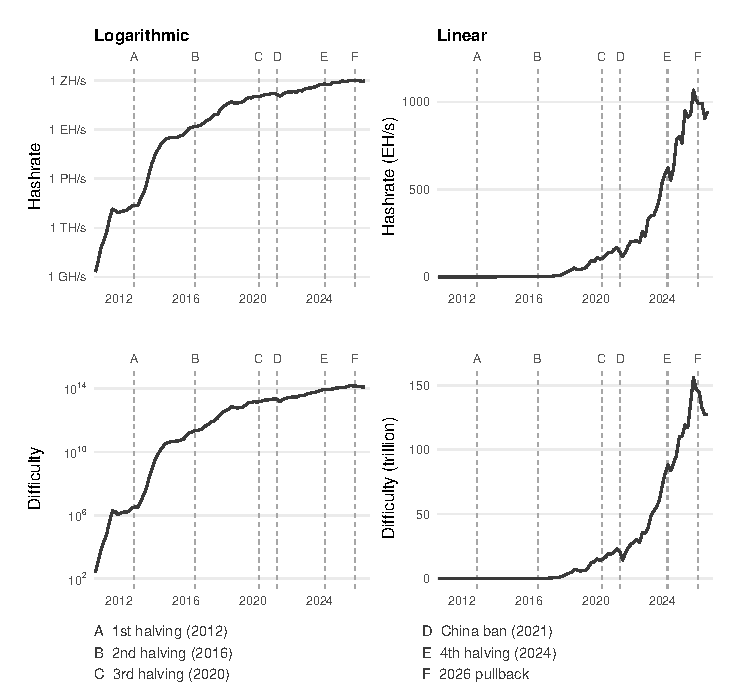
\includegraphics[width=\textwidth]{images/network_hr_diff_v2}
  \caption{
    Bitcoin network hashrate and difficulty on logarithmic scales (left) and linear scales (right). The logarithmic view spans gigahashes to zettahashes per second; the linear view shows the absolute size of rises and falls. Dashed lines mark the four halvings, the China ban and the 2026 pullback, identified by the shared key. Lines join sampled observations, which can miss short-lived peaks and troughs. Data: Braiins Insights API \autocite{BraiinsInsights}. % fig-src: analysis/figures/fig_ch1_network_hr_diff.R
  }
  \label{fig:network-hashrate-difficulty}
\end{figure}

Hashrate and mining difficulty exhibit a near-perfect correlation over Bitcoin's history because increased hashrate directly triggers increased difficulty. Technological advancements, competitive economic incentives, and growing participation have driven a long-term rise in both hashrate and difficulty. The trend is not monotonic, though: as the figure shows, hashrate retreated in 2026 from a peak of roughly 1{,}100~exahashes per second (EH/s) reached in late 2025. % src: analysis/checks/ch1_hashrate_peak.R on analysis/data/network_hashrate_daily.csv in 7-day means, the estimator of the 930 EH/s below: peak 1,132.7 EH/s in the week to 2025-10-20 (daily max 1,151.5 on 2025-10-18), 2026 high 1,070.1 in the week to 2026-03-02; the figure plots braiins_hashrate_difficulty_all.json, one point about every 62 days, whose top point is 1,067.6 EH/s on 2025-11-08, inside late 2025; CoinSharesMiningQ12026 (read 2026-09-26): peak approximately 1,160 EH/s in early October 2025; the 1,086 EH/s Feb 2026 high this note cited until 2026-09-26 came from a live fetch no committed file reproduces

Several major events are annotated in the graph:

\begin{itemize}
  \item \textbf{Halvings (2012, 2016, 2020, 2024)}: These occur approximately every four years and reduce the block subsidy, the newly minted part of the block reward, by half, decreasing the issuance rate of new bitcoins.

  \item \textbf{China Mining Ban (June 2021)}: The Chinese government banned Bitcoin mining operations, prompting a large-scale migration of hashrate out of the country. This resulted in a sharp drop in both hashrate and difficulty, followed by a gradual recovery as miners relocated to new jurisdictions such as North America.

  \item \textbf{2026 Pullback}: The decline visible at the right edge of the graph. A weakening bitcoin price squeezed mining margins, and several of the largest mining operators began redirecting sites and grid capacity from Bitcoin mining toward AI and high-performance-computing workloads \autocite{CoinSharesMiningQ12026,CoreScientificQ22026,TeraWulfQ22026}. % src: CoinShares Q1 2026 (hashprice ~$63 to ~$28-30/PH/day Jul 2025-Mar 2026; >$70bn announced AI/HPC contracts across listed miners); Core Scientific Q2 2026 (colocation $136.7M vs self-mining $21.5M); TeraWulf Q2 2026 (HPC lease = 71% of revenue)
\end{itemize}

Other milestones, not directly labeled in the graph, include:

\begin{itemize}
  \item \textbf{ASIC Adoption (2013--2016)}: ASIC miners were first introduced in early 2013 (the first was the Avalon ASIC Batch 1), outperforming previous GPU and FPGA mining solutions. By 2015, ASIC dominance was complete. Mining shifted toward industrial-scale operations, and network hashrate, and thus mining difficulty, skyrocketed.

  \item \textbf{Global Expansion (2017--2020)}: Driven by rising concerns over regulatory risks and centralization in China, miners increasingly expanded to regions with favorable electricity costs and regulations. This led to substantial investment in mining infrastructure in the United States and Russia, decentralizing Bitcoin mining geographically.

  \item \textbf{Post-2021 Era}: China's ban redistributed mining capacity globally \autocite{Reuters2021,CCAF2021}, and public scrutiny of mining's environmental impact intensified, pushing operators toward renewable energy. At the same time, miners deployed far more efficient hardware (Bitmain's Antminer S19 and later S21 series), which kept hashrate growing even as margins tightened.
\end{itemize}

\section{Electricity as the Primary Mining Expense}

Electricity is mining's biggest ongoing cost. Running hundreds or thousands of mining machines 24/7 consumes enormous amounts of power, and cooling those machines to prevent overheating adds even more to the bill.

Because of this, miners are obsessed with energy prices. Profitability boils down to a simple equation: the value of the bitcoin you earn versus the cost of the electricity you use to earn it. If your electricity costs are too high, you could end up spending more on power than you make in bitcoin. Successful miners chase an all-in (delivered) rate of five cents per kilowatt-hour (kWh) or less, \$50 per megawatt-hour (MWh) in this book's units, by setting up shop in regions with cheap power or striking deals for industrial rates \autocite{CBECI2026,riot2026q1prod}. In 2025 a large West Texas mine buying at the real-time price would have paid about \$51 a megawatt-hour before its retail adder: \$42 of energy and \$9 of transmission, losses, reserves and fees (Chapter~6). Some miners even pause their machines during price spikes, and some are paid by the grid to curtail, through programs called demand response. % src: CBECI2026 methodology page, Assumption 1 (read 2026-09-27): "The average electricity price for bitcoin mining globally is constant over time and is 0.05 USD/kWh", the five cents of sec:bitcoin_consumption_own_computation; riot2026q1prod (read 2026-09-27): "All-in Power Cost - Total" 3.0c/kWh for Q1 2026 (3.8 in Q1 2025), its note 7: estimated, "Inclusive of all transmission and distribution charges, fees, adders, and taxes", and net of total power credits; 5 cents/kWh = $50/MWh; analysis/checks/ch6_btm_ledger.R console (re-run 2026-09-27), the chapter 6 table tab:btm-ledger: 100 MW at transmission voltage in Oncor's territory, 2025, 95% capacity factor; energy 42.18 = LZ_WEST 2025 mean real-time settlement point price (ERCOT MIS 13061, analysis/data/ercot_rtm15_spp_loadzones_2021on.csv.gz, the book's anchor); non-energy stack 8.83 = losses 0.91 + ancillary 0.39 + uplift including ERCOT's fee 1.38 + Rider TCRF 5.65 + distribution 0.50; delivered 51.01 with no 4CP avoidance, 45.35 with all four peaks avoided, both rows of the table; a modelled site, not an observed bill, and the retail supplier margin is excluded (private), so the $51 is printed as before the retailer's adder, unlike Riot's all-in figure, which includes adders; until 2026-09-27 this line printed "as low as $0.05 per kilowatt-hour", unsourced, and "far below what most households pay", dropped because nothing sourced it (EXEC-040)

Over time, mining settles into a balance where only those with the cheapest power and best hardware stay in the game. This drives miners to places with abundant energy, like hydroelectric dams in Canada or geothermal plants in Iceland, or even to use \glossaryterm{stranded-energy}{stranded energy} that would otherwise go unused: power generated where no transmission line or nearby customer can take it, such as the gas that oil fields would otherwise burn off in flares. Texas, whose grid this book examines in depth, has become one of the biggest of these destinations.

\subsection*{A Closer Look: Inside an Antminer S21~XP}

To understand why Bitcoin mining is so energy intensive, look inside a modern mining machine. Take the Antminer S21~XP, the air-cooled machine used throughout this book.
The device consists of:

\begin{itemize}
\item Hashboards lined with the ASIC chips that do the hashing
\item One control board
\item One power supply unit (PSU)
\item High-speed fans for cooling both the hashboards and the PSU
\end{itemize}

Bitmain rates the machine at 270 terahashes per second (TH/s). Its power rating is measured at the wall and covers the chips, the fans, the control board and the power supply's own conversion losses \autocite{bitmain2024s21xp,braiinsacademytechres}. % src: bitmain2024s21xp and braiinsacademytechres, checked 2026-09-28: air-cooled S21 XP stock hashrate 270 TH/s, power on wall 3,645 W, efficiency 13.5 J/TH; highest-rated air-cooled S21 XP variant in the supplied Braiins table, distinct from XP Hyd and XP Imm. Firmware target limits are not stock ratings.

\[
\fbox{\textbf{3{,}645~W at the wall}}
\]

For comparison:
\begin{quote}
\textit{The amount of electricity an average American household consumes over an entire day \autocite{EIAHouseholdConsumption2022}, used by a single miner in just eight hours.} % src: EIA FAQ id=97, read 2026-09-25: 10,791 kWh per residential customer in 2022 = 29.6 kWh a day; 29.6 kWh / 3.645 kW = 8.1 h. The earlier "six high-end gaming PCs" comparison had no source and was cut
\end{quote}

Industrial-scale mining farms often deploy thousands of these machines. A single site with 1{,}000 S21~XP units would require about 3.6 megawatts of power for the miners alone. % src: 1,000 x 3,645 W = 3.645 MW (bitmain2024s21xp); excludes site overhead.

\phantomsection\label{par:ch1-efficiency}Dividing power draw by hashrate gives the machine's \glossaryterm{efficiency}{efficiency}: $3{,}645~\text{W} / 270~\text{TH/s} = 13.5$ joules per terahash (J/TH), Bitmain's own rating. % src: bitmain2024s21xp (power efficiency on wall at 25 C: 13.5 J/TH)
Efficiency is the single most important specification of a mining machine, and the industry's progress is easiest to read in its steady fall: a decade ago the workhorse Antminer S9 needed roughly 100~J/TH, the S21~XP examined above needs 13.5, and the latest liquid-cooled (hydro) machines have pushed below 10 (Figure~\ref{fig:asic-efficiency}). % src: analysis/data/bitmain_flagship_efficiency.csv, one Bitmain document per row: S9 launched May 2016 (Bitmain news, July 24, 2019), 14 TH/s at 1,400 W on its spec page = 100 J/TH; S21 XP 13.5 J/TH (bitmain2024s21xp); S23 Hyd 580 TH/s at 9.5 J/TH (about 5,510 W), launched at WDMS 2025, Las Vegas, May 26-27, 2025, shipping from Q1 2026 (Bitmain on X, May 27, 2025); S23 XP Hyd 600 TH/s at 8.9 J/TH (5,340 W), launched at WDMS Global 2026, Hong Kong, August 28, 2026, shipping from November 2026 (BITMAIN Shop product page, read 2026-10-12; row in the same CSV), the lowest point of the figure
Efficiency will return throughout this book, because it sets the electricity price at which a given machine stops being profitable.

\begin{figure}[h]
  \centering
  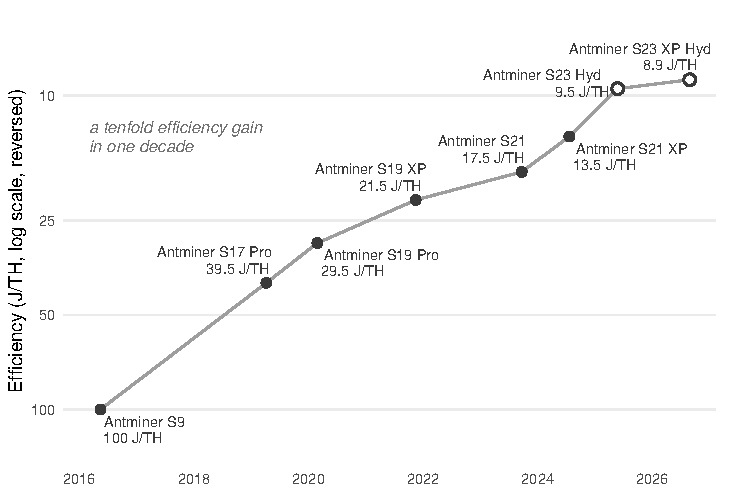
\includegraphics[width=\textwidth]{images/asic_miner_eff}
  \caption{
    ASIC miner efficiency over time: a selection of Bitmain's Antminer models at their rated efficiency at the wall on stock settings, each placed at its announcement or launch date except the air-cooled S21~XP, dated to its published specification. Lower means less energy per unit of computation; the axis is logarithmic and reversed, so the steady multiplicative gains read as a straight climb. Open points are hydro (liquid-cooled) models; filled points are air-cooled. Data: Bitmain specification pages and launch announcements, listed point by point in the companion repository. % fig-src: analysis/figures/fig_ch1_asic_efficiency.R, reading analysis/data/bitmain_flagship_efficiency.csv (one Bitmain document per point, read 2026-09-25)
  }
  \label{fig:asic-efficiency}
\end{figure}

\section[How Much Power Does Bitcoin Mining Use?]{How Much Power Does Bitcoin\\ Mining Use?}
\label{sec:bitcoin_consumption_own_computation}

To estimate the Bitcoin network's total power consumption, you need two key figures: the network's total computational throughput (hashrate) and the average energy efficiency of the mining hardware. As of August 2026, the Bitcoin network's hashrate is approximately 930~EH/s (930,000,000~TH/s) \autocite{BraiinsInsights}. % src: hashrate = 930.2 EH/s, the 7-day mean to 2026-08-21 of the committed daily cache analysis/data/network_hashrate_daily.csv (Braiins Insights global series), rounded; analysis/checks/ch1_network_energy.R reads both committed caches (analysis/data/network_hashrate_daily.csv, analysis/data/btc_price_daily.csv), 7 days to 2026-08-21. Until 2026-09-25 this cited an uncommitted live fetch of that day (927.8 EH/s)
That figure is inferred rather than counted, because nobody sees the hashes themselves: on average a block takes the difficulty times $2^{32}$ hashes to find, so dividing that by the observed time between blocks gives the network's hashrate, and a daily figure moves with the luck of how quickly that day's blocks happened to arrive \autocite{stoll2018ceepr}. % src: stoll2018ceepr p. 5 ("As each block has about 2^32 hashes, and one block is solved every 10 minutes", hashrate = difficulty x 2^32 H / 600 s); added 2026-10-12 after a review comment asking how network hashrate is estimated
The second figure is harder, because nobody measures it. Difficulty tells you how many hashes the network performs, not how many watts they cost: the protocol checks that the work was done and records nothing about the electricity it took. Every published estimate of Bitcoin's power use therefore rests on an assumption, most often an efficiency that someone modeled, and dividing such an estimate back by the hashrate returns only that assumption. % src: CCAF2025 p. 60 ("Methodologies for Estimating Electricity Consumption", four approaches, of which none measures the whole network: the top-down approach, "This widely adopted method", multiplies the implied hashrate by the assumed efficiency of a representative device; the economic approach estimates consumption "at the break-even point where mining revenue equals operational costs"; the hybrid top-down approach, CBECI's, computes the efficiency of a hypothetical device from hardware that meets a profitability threshold; extrapolation from direct measurement of "a small, representative portion of the network"; the economic approach assumes miners' operating costs, the extrapolation assumes the sample is representative; until the DATA-017 review, 2026-09-26, this sentence said every estimate multiplies the hashrate by a modelled or assumed efficiency, which the economic approach does not); CBECI2026 (FAQ, verbatim: "Bitcoin's real electricity consumption cannot be directly measured"; methodology: power = hashrate x the efficiency of a weighted basket of profitable hardware models x a PUE); protocol: the expected hashes per block are difficulty x 2^32, so difficulty fixes the hashrate and nothing on chain records power

What is published covers part of the network. Twelve fleets run by listed mining companies report their efficiency. In mid-2026 they had about 345~EH/s between them, more than a third of the network on the companies' own capacity figures, and they averaged 17~J/TH, weighted by hashrate \autocite{mara10q2026q2,bitdeer2026q2,cleanspark2026aug,riot2026q1prod}. % src: analysis/checks/ch1_fleet_efficiency.R console, section 1: 12 fleets of 11 companies, 345.1 EH/s = 37.1% of the anchor's 930.2 EH/s, 16.98 J/TH hashrate-weighted (16.65 to 17.95 across the script's variants); analysis/data/listed_miner_fleets_2026.csv, one row per fleet with its document, URL and a verbatim quote, every source re-read 2026-09-26; the four cited documents give the four largest, 235.8 EH/s: MARA 70.3 EH/s at 17.3 J/TH, Bitdeer 73.0 at 15.8, CleanSpark 50 at 16.07, Riot 42.5 at 20.2 (Riot's latest J/TH, from March)
That segment is self-reported, often from the machines' ratings rather than meters, and it leans toward efficient machines. Listed companies have the capital for the newest machines, two of them make their own, and some report the efficiency of only the machines they run, leaving out the older ones they own but have switched off. % src: analysis/data/listed_miner_fleets_2026.csv basis columns and row notes: MARA's energized hashrate assumes every operational rig is "running at 100% of manufacturers' specifications" (its 10-Q for the quarter to June 30, 2026, verbatim; row note: "Unaudited, rating-based, not metered"); Riot's fleet efficiency is "unaudited, estimated"; BitFuFu's 16.7 J/TH equals 344 MW / 20.6 EH/s, power capacity over hashrate; Bitdeer's SEALMINER and Canaan's Avalon machines; American Bitcoin's ~14.1 J/TH covers its ~58,999 operating miners of ~89,242 owned; TeraWulf's 16.4 covers its operational 5.6 EH/s of 10.6 nameplate, its whole fleet averaging 17.6

One published model of the whole fleet comes from the University of Cambridge. Nobody publishes how many of each machine were sold, so Cambridge's index takes every model still profitable at five cents a kilowatt-hour and weights it by its age; on September 25, 2026 it put the network's machines at 17.0~J/TH \autocite{CBECI2026}. % src: CBECI2026, model v1.8.0, values for 2026-09-25 read 2026-09-26: hardware efficiency 17.013 J/TH best guess (bounds 9.50 and 30.00 J/TH), power 17.12 GW with PUE 1.10 (8.78 and 32.93 GW); methodology: 0.05 USD/kWh (Assumption 1), release-date weights from 1 to 0 in steps of 0.2; FAQ: "no reliable sales or distribution figures"; quoted from CCAF material licensed CC BY-NC-SA 4.0, no CCAF data in the repository (analysis/checks/ch1_fleet_efficiency.R section 4 holds the quoted figures); until 2026-10-10 "The one published model": Coin Metrics Labs also publishes a fleet estimate (MINE-MATCH, labs.coinmetrics.io), not read or cited here
I read the model, like the listed segment, as likely to overestimate the fleet's efficiency in a lean year. Cambridge has set the model three times against miners' own reports of their fleets, and the reports have run from 3~percent more efficient than the model, in June 2022, to 11~percent less efficient, in June 2024. Cambridge expects the model to read the fleet as more efficient than it is when margins are thin \autocite{CCAF2025}, and in 2026 they were \autocite{CoinSharesMiningQ22026}. Scaled by those gaps, its 17.0 becomes 16.5 to 19.0~J/TH. % src: CCAF2025 p. 59, Figure 26(b): Bitcoin Mining Council surveys 40.6 against the model's 41.8 J/TH (June 2022) and 36.9 against 34.5 (June 2023), the CCAF survey 28.2 against 25.3 (June 2024; 45 of the survey's 49 firms, Figure 26 "Sample size: (N=45)", the survey as a whole covering nearly 48% of hashrate, pp. 9-10 and Figure 18; hashrate-weighted, which the report says leans toward the larger, more efficient firms); "CBECI estimates generally indicate slightly less efficient hardware during periods of high mining profitability and vice versa"; the direction for 2026 is the author's reading, the size is not known; CoinSharesMiningQ22026 section 1: Q2 2026 "pushed the listed mining sector below cash breakeven in aggregate", monthly average hashprice at an all-time low of $27.7/PH/s/day in June; analysis/checks/ch1_fleet_efficiency.R section 4: ratios 0.971 / 1.070 / 1.115 x 17.013 = 16.5 to 19.0 J/TH

The unknown is the rest of the network, the three-fifths that publishes no efficiency, and this book states it as a range. If the rest were nearly as efficient as the listed fleets, about 18.6~J/TH, the network would average 18; if it ran S19~Pro-class machines or worse, about 31~J/TH, it would average 26. This book takes that span, 18 to 26~J/TH at the machines, as its result. Both ends are my judgments; the listed fleets and Cambridge's model only check them. % src: analysis/checks/ch1_fleet_efficiency.R console, section 1: the rest (62.9% of 930.2 EH/s) must average 18.6 J/TH for an 18 J/TH network and 31.3 for 26 (18.4 and 29.9 if the listed share of hashes delivered is only 30%); reference machines from analysis/data/bitmain_flagship_efficiency.csv: S19 Pro 29.5, S19 XP 21.5, S21 17.5 J/TH; the range replaces the single assumed 26 J/TH of the earlier text (DATA-017, author decision 2026-09-26)

Inside that range, my own estimate is 21.5~J/TH, and it might be even lower. It is a judgment, not a measurement; it puts the rest at about 24~J/TH, and the worked example below uses it. The top of the range, 26~J/TH, would mean the fleet had made no progress since 2024: Cambridge's model already read the network's machines at 25.3~J/TH in June 2024 and at 23.7 by that December \autocite{CCAF2025}. % src: author decision 2026-09-26 (DATA-017): 21.5 J/TH is the author's current estimate, and 26 J/TH, the book's single figure until then, was set before about March 2025 (more than 1.5 years before 2026-09-26, per the author's decision of that day, which also calls it a figure for an older fleet; the prose now states that as what 26 would imply rather than as book-making history); analysis/checks/ch1_fleet_efficiency.R section 1: rest 24.2 J/TH at the listed 37.1% (23.4 at 30%); CCAF2025 pp. 59 and 63 (CBECI hardware efficiency 25.3 J/TH on 2024-06-30 and 23.7 by the end of December 2024, the book's machine basis)

Profitability puts a ceiling on the range; it cannot confirm it. At the August 2026 bitcoin price of roughly \$66{,}000 and that month's hashrate, the block subsidy pays miners about \$0.032 a day per TH/s of hashrate. % src: 450 BTC/day (144 blocks x 3.125 BTC) x $66,180 / 930.2M TH/s = $0.03202; analysis/checks/ch1_network_energy.R reads both committed caches (analysis/data/network_hashrate_daily.csv, analysis/data/btc_price_daily.csv), 7 days to 2026-08-21; transaction fees excluded (currently a low single-digit percent addition). Printed $67,000 and $0.033 until 2026-09-25, from an uncommitted fetch ($67,076, 927.8 EH/s) the repository could not reproduce
A machine paying \$50 per megawatt-hour for electricity therefore breaks even at about 27~J/TH, and one paying \$40 at about 33~J/TH; Chapter~4 derives this breakeven arithmetic in full. Machines less efficient than the breakeven for their power price mine at a loss and, sooner or later, shut down, so the operating fleet's average must sit below it. Cambridge's index draws the top of its own estimate with the same arithmetic, so the two agreeing would prove nothing. % src: analysis/checks/ch1_network_energy.R console: $0.03202/TH-day subsidy hashprice; breakeven 26.7 J/TH at $50, 33.4 at $40; 18 / 21.5 / 26 J/TH stay under the bound for a fleet paying up to $74.1 / $62.0 / $51.3 per MWh; CBECI2026 methodology: the upper bound is the least efficient model still profitable at the assumed price, times the hashrate and a PUE of 1.20; until 2026-09-26 this paragraph called the bound a sanity check that supported 26 J/TH

The site's meter lowers the ceiling further: besides the machines, it counts the site's cooling and transformer losses, a tenth more than the machines draw in Cambridge's central case \autocite{CBECI2026}. At \$42 per megawatt-hour, the 2025 average real-time price in ERCOT's West load zone (Chapter~4), a network averaging 18~J/TH would have spent about 62~percent of its August 2026 revenue on electricity, including that additional tenth. At my estimate of 21.5~J/TH, the share would have been about three-quarters; at 26~J/TH, about nine-tenths. % src: $42.18 = mean of the 35,040 15-minute real-time settlement point prices of LZ_WEST in 2025, ERCOT MIS report 13061 (analysis/data/ercot_rtm15_spp_loadzones_2021on.csv.gz; chapter-4.tex sec:sensitivity, the book's reference price, author decisions 2026-08-24 and 2026-09-04); analysis/checks/ch1_fleet_efficiency.R console, section 3 (hashprice $0.03223 per TH-day with August's 0.67% fee share; PUE 1.10, CBECI2026 methodology Assumption 8): at $42.18, 18 J/TH 62%, 21.5 J/TH 74%, 26 J/TH 90%; at PUE 1.01 the same are 57 / 68 / 82%
Six listed miners, from the efficient end of the network, spent 58~percent of their second-quarter mining revenue on electricity after curtailment credits, which would be about three-fifths at August's lower revenue per terahash \autocite{CoinSharesMiningQ22026}. Neither end is ruled out: Cambridge suggests its survey's least efficient fleets run on exceptionally cheap power \autocite{CCAF2025}, and at \$35 per megawatt-hour even 26~J/TH takes only three-quarters of revenue. % src: analysis/data/listed_miner_power_share_2026.csv (CoinShares Q2 2026 section 5.2, six fleets, 10,561 BTC: electricity net of credits 58.3% of realised revenue, BTC-weighted; Riot's and MARA's rows checked against their own documents, MARA's including hosting fees); analysis/checks/ch1_fleet_efficiency.R section 3: period-matched 61.3% on the subsidy basis (Q2 hashprice $0.03389 against the anchor's $0.03223), 59.0% on Braiins' hashprice series; 26 J/TH at $35 and PUE 1.10: 75%; CCAF2025 p. 59, on the survey's unweighted mean of 30.6 J/TH against its median of 29.5: "A plausible explanation could be the operation of older devices in regions with exceptionally low electricity costs"

\noindent Using the basic formula:
\[
\text{Power (W)} = \text{Hashrate (TH/s)} \times \text{Efficiency (J/TH)}
\]

you get, at my estimate of 21.5~J/TH and across the range:
\begin{align*}
930{,}000{,}000~\text{TH/s} \times 21.5~\text{J/TH} &= 19{,}995{,}000{,}000~\text{W} \approx 20.0~\text{GW}\\
930{,}000{,}000~\text{TH/s} \times (18\text{--}26)~\text{J/TH} &= \boxed{16.7 \text{ to } 24.2~\text{GW}}
\end{align*}

To estimate annual electricity usage:
\begin{align*}
19.995~\text{GW} \times 24 \times 365 &\approx 175~\text{TWh/year}\\
(16.74 \text{ to } 24.18)~\text{GW} \times 24 \times 365 &\approx \boxed{147 \text{ to } 212~\text{TWh/year}}
\end{align*}

These figures are the machines' own draw. At the grid meter, including the additional tenth for cooling and transformer losses in Cambridge's central case, the same range is 18.4 to 26.6~GW, or 161 to 233~TWh a year. % src: analysis/checks/ch1_network_energy.R console at 930 EH/s: 21.5 J/TH = 19,995,000,000 W = 20.0 GW x 8,760 h = 175.2 TWh/yr; 18 J/TH = 16.74 GW = 146.6 TWh/yr; 26 J/TH = 24.18 GW = 211.8 TWh/yr, boxed as 16.7 to 24.2 GW and 147 to 212 TWh (from the unrounded 16.74 GW; the rounded 16.7 x 8.76 gives 146.3); analysis/checks/ch1_fleet_efficiency.R section 2: x PUE 1.10 (CBECI2026 Assumption 8) = 18.4 to 26.6 GW, 22.0 at 21.5 J/TH; TWh at meter 161.3 / 192.7 / 233.0 at 18 / 21.5 / 26 J/TH (also analysis/checks/ch1_network_energy.R, "at the meter" line); until 2026-09-26 the chapter assumed 26 J/TH (24.2 GW, 212.0 TWh) and printed 22 to 30 J/TH as its range

\begin{figure}[h]
  \centering
  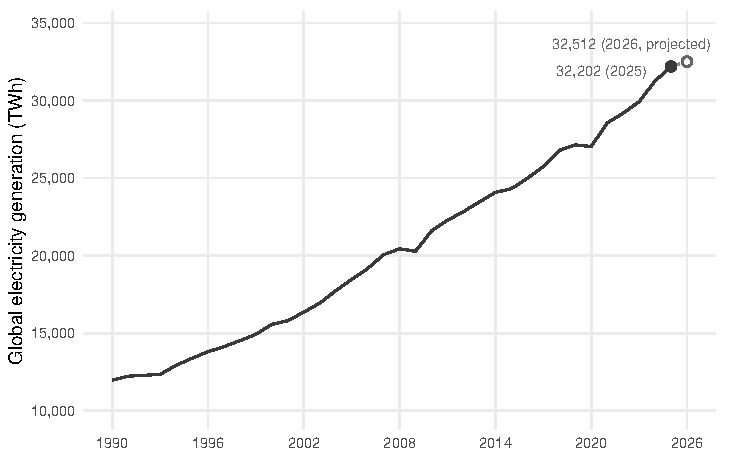
\includegraphics[width=\textwidth]{images/global_generation}
  \caption{
    Global electricity generation, 1990--2025 actuals with 2026 projected from the 2016--2025 trend. Data: Energy Institute Statistical Review of World Energy \autocite{EIStatReview2026}, 1990--2023 series as republished by Statista \autocite{StatistaGlobalGeneration2024}. % fig-src: analysis/figures/fig_ch1_global_generation.R
  }
  \label{fig:global_generation}
\end{figure}

Compare this August 2026 run-rate at the machines with global electricity generation, which reached approximately 32,202~TWh in 2025, the latest full year \autocite{EIStatReview2026}. Bitcoin mining represents:
\[
\frac{147 \text{ to } 212~\text{TWh}}{32{,}202~\text{TWh}} \times 100 \approx \boxed{0.46 \text{ to } 0.66\%~\text{of 2025 global generation}}
\]

At my 175~TWh it is 0.54~percent; at the meter, the like-for-like basis, 0.50 to 0.72~percent. % src: analysis/checks/ch1_network_energy.R console: at the machines 146.6 / 32,202 = 0.46%, 211.8 / 32,202 = 0.66%, 175.2 / 32,202 = 0.54% (the network power table); "at the meter" line (PUE 1.10): 161.3 / 32,202 = 0.50%, 233.0 / 32,202 = 0.72%, 192.7 / 32,202 = 0.60%; machines first by author decision 2026-09-27; numerator an August 2026 run-rate, denominator 2025 generation, hence the box label
By comparison, data centers used about 415~TWh in 2024, roughly 1.5~percent of global electricity consumption \autocite{IEADataCenters}. The IEA counts Bitcoin mining outside that total. % src: IEA, Energy and AI (10 April 2025), executive summary: "Data centres accounted for around 1.5% of the world's electricity consumption in 2024, or 415 terawatt-hours (TWh)". Scope: full report PDF p.71 n.2 and p.72 place cryptocurrencies (primarily Bitcoin mining, about 125 TWh in 2023, 0.5% of global electricity) outside the ICT and data centre boundary, so the 415 TWh does not double-count the 147 to 212 TWh (161 to 233 at the meter) above; the like-for-like pair is the meter figure, since both are whole-site figures (the IEA's data-centre consumption counts cooling and other infrastructure with the servers, Energy and AI p. 52: "The share of cooling systems in total data centre consumption varies from about 7% ... to over 30%", and its consumption chart splits servers, other IT, cooling and other infrastructure; the chapter's figure is at the sites' meters); the IEA's crypto figure is itself "IEA analysis based on data from ... Cambridge Centre for Alternative Finance (2025), and company reports" (Figure 2.15 sources, the CCAF entry being CBECI), so it is not a check on this chapter's range independent of CBECI2026. The earlier IEA figure of 460 TWh in 2022 (Electricity 2024) does bundle crypto and is not used here.

\chapter{How Power Systems Work and Why Balance Matters}
\chaptermark{How Power Systems Work}

Imagine your regional electric grid as a huge, humming engine. Complicated as it is, its fundamental job is balance: keeping exactly the right amount of power flowing at every moment. This chapter explains how power systems work, why that balance matters, and how Bitcoin mining can help maintain it.

\section{Electric Power System Basics}

Electric power systems have three main components: generation, \glossaryterm{transmission}{transmission}, and \glossaryterm{distribution}{distribution} (delivery to loads, the consumers of power). In simple terms, power plants generate electricity, step-up transformers raise it to high voltage, transmission lines carry it over long distances, and lower-voltage distribution networks finally deliver it to homes and businesses. Generation refers to producing electricity from energy sources (for example, burning natural gas or harnessing wind in a turbine). Transmission is the bulk transport of electricity at high voltages over regional distances (the tall tower lines you see crossing the countryside). High voltages are used because they allow efficient long-distance transfer with minimal losses. Distribution is the local delivery of power at lower voltages, after transformers step down the voltage, to neighborhoods, businesses, and individual consumers.
The largest consumers usually skip that last step. A mine of the size this book prices, like the 100~MW site of Chapter~\ref{ch:buying}, takes its power straight from the transmission system through its own substation. In the territory of Oncor, a Texas transmission and distribution utility, that means delivery above 60,000 volts \autocite{oncor2026retailtariff}. % src: oncor2026retailtariff sec. 6.2.2 Standard Voltages, p. 164 ("Transmission voltage is any one of the Company's standard voltages in excess of 60,000 volts"; standard transmission voltages 69, 138 and 345 kV) and sec. 6.1.1.1.7 Transmission Service, p. 80; "a substation of its own" is not the tariff's phrase but follows from its definitions on p. 164: primary voltage is delivery "after one Company transformation ... from a transmission voltage", while transmission-voltage delivery has no Company transformation, so the step-down transformer is the customer's; chapter 6 tab:btm-ledger (100 MW at transmission voltage in Oncor's territory)
Load (or demand) denotes the electricity being consumed by end-users: all the lights, appliances, machines, and devices drawing power at any given moment. All these pieces together form what's commonly called the grid, an interconnected network linking producers and consumers of electricity \autocite{EIAElectricDelivery}.

\begin{figure}[h]
    \centering
    \resizebox{\textwidth}{!}{% Original diagram (it replaced an unattributed PNG, since deleted).
% Generation -> transmission -> distribution -> load chain with
% step-up/step-down transformers drawn as overlapping circles, plus the
% transmission-level tap that serves large sites (mines, data centers,
% heavy industry) through their own step-down substation.
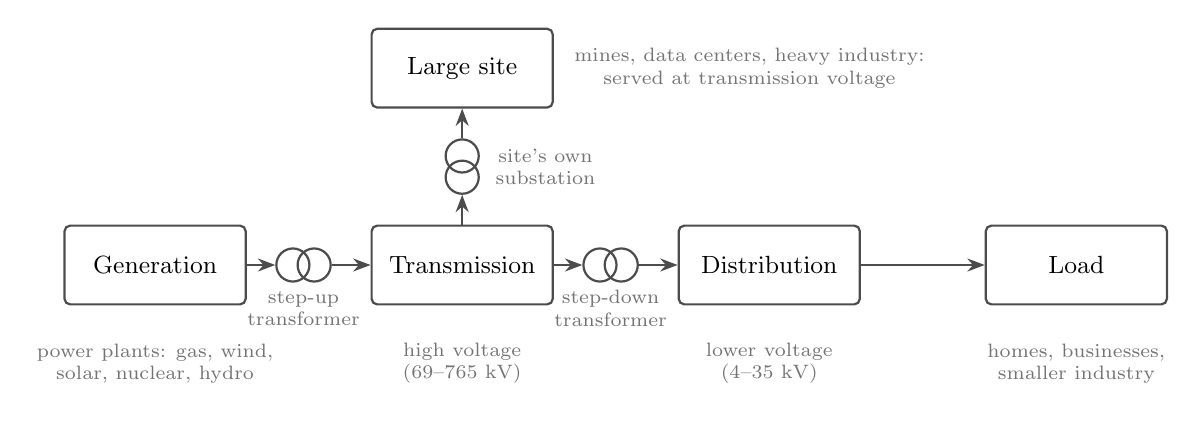
\begin{tikzpicture}[
  font=\small,
  stage/.style={draw=black!70, rounded corners=2pt, thick, align=center,
                minimum height=10mm, minimum width=23mm},
  xfmr/.style={circle, draw=black!70, thick, minimum size=4.2mm, inner sep=0pt},
  arr/.style={-{Stealth[length=2.2mm]}, thick, black!70},
  note/.style={font=\scriptsize, text=black!55, align=center}
]
  \node[stage] (gen)  at (0,0)    {Generation};
  \node[stage] (tx)   at (3.9,0)  {Transmission};
  \node[stage] (dist) at (7.8,0)  {Distribution};
  \node[stage] (load) at (11.7,0) {Load};
  \node[stage] (big)  at (3.9,2.5) {Large site};

  % step-up transformer between generation and transmission
  \node[xfmr] (t1a) at (1.75,0) {};
  \node[xfmr] (t1b) at (2.02,0) {};
  \draw[arr] (gen) -- (t1a);
  \draw[arr] (t1b) -- (tx);
  \node[note] at (1.885,-0.55) {step-up\\transformer};

  % step-down transformer between transmission and distribution
  \node[xfmr] (t2a) at (5.65,0) {};
  \node[xfmr] (t2b) at (5.92,0) {};
  \draw[arr] (tx) -- (t2a);
  \draw[arr] (t2b) -- (dist);
  \node[note] at (5.785,-0.55) {step-down\\transformer};

  \draw[arr] (dist) -- (load);

  % transmission-level tap: the large site's own step-down substation
  \node[xfmr] (t3a) at (3.9,1.115) {};
  \node[xfmr] (t3b) at (3.9,1.385) {};
  \draw[arr] (tx) -- (t3a);
  \draw[arr] (t3b) -- (big);
  \node[note, anchor=west] at (4.2,1.25) {site's own\\substation};

  % stage annotations
  \node[note] at (0,-1.25)    {power plants: gas, wind,\\solar, nuclear, hydro};
  \node[note] at (3.9,-1.25)  {high voltage\\(69--765 kV)};
  \node[note] at (7.8,-1.25)  {lower voltage\\(4--35 kV)};
  \node[note] at (11.7,-1.25) {homes, businesses,\\smaller industry};
  \node[note, anchor=west] at (5.2,2.5) {mines, data centers, heavy industry:\\served at transmission voltage};
\end{tikzpicture}
}
    \caption{Simplified diagram of an electric power system: generation, transmission, and distribution deliver electricity to loads. Large sites, mines among them, take their power straight from the transmission system through a substation of their own.}
    \label{fig:power_system}
\end{figure}

Because our society relies on electricity, power systems are designed with reliability in mind. Most local grids are tied together into larger networks so they can support each other. For example, utilities interconnect their systems so that if one area has a shortage or an outage, power can be rerouted from elsewhere to compensate. In North America, virtually all generators within a vast region operate synchronously as part of large interconnections (Eastern, Western, and Texas interconnections in the U.S.). This means the entire grid in each region runs at the same electrical frequency (60~Hz in the United States), and power can flow across state or regional lines as needed. These interconnections and built-in redundancies help ensure that failures (like a single power plant or line tripping offline) do not immediately lead to widespread outages. The grid is a single huge machine with many parts working together to keep your lights on.

\section{Balancing Supply and Demand in Real Time}

Electricity supply must always match demand in real time. Unlike some other commodities, electricity cannot be easily stored in large quantities (at least not yet on the scale of the whole grid), so generation and load must be balanced every second of every day. If consumers collectively need, say, 30,000 megawatts (MW) at a given moment, the connected power plants must produce roughly 30,000~MW in that moment. If generation and consumption fall out of balance, even for a short time, the stability of the grid is jeopardized. Grid operators (sometimes called balancing authorities) are responsible for monitoring this balance and adjusting generation output or shifting loads as needed to keep the two in sync.

The \glossaryterm{utility-frequency}{utility frequency} is a key indicator of that balance. In a synchronized AC grid, frequency is the number of alternating current cycles per second, measured in hertz (Hz). In the U.S., the standard frequency is 60~Hz, while in many other countries it is 50~Hz. When generation exceeds demand, the grid frequency will rise above its target (generators speed up); if demand exceeds generation, the frequency will drop below 60~Hz (generators slow down). The direction of frequency change reveals the imbalance. Frequency can settle below or above its target once supply and demand match again; returning it to the target takes a further control action. Operators use control systems and operating reserves to hold frequency very close to the 60~Hz setpoint at all times \autocite{NERCBalancingFrequency2021}.

\section{Slowing the Fall and Stopping It}
\label{sec:inertia}

When a big power plant trips offline, its output vanishes in an instant, but the frequency does not collapse in that instant.
The big synchronous generators on the grid (gas, coal, nuclear, hydroelectric) are several thousand tons of metal spinning in lockstep with all the others, often at 3,600 revolutions per minute, and that spinning mass stores energy \autocite{FERCNERCFeb2021,ercot2024asstudy}. % src: FERCNERCFeb2021 appendix E, appendix p. 19 (PDF p. 263): "synchronous generators are several thousand tons of mass in motion, often rotating at 3,600 revolutions per minute (at 60 Hz)"; ercot2024asstudy p. 25 (inertia "inherently provided by synchronous generators, such as gas, coal, nuclear, and hydro")
That stored energy is the grid's \glossaryterm{inertia}{inertia}: in the first seconds after a trip, the missing power is drawn out of the rotating machines themselves, they slow down, and the frequency falls with them \autocite{ercot2018inertia,NERCBalancingFrequency2021}. % src: ercot2018inertia p. 4 ("kinetic energy will automatically be extracted from the synchronous machines, causing them to slow down"); NERCBalancingFrequency2021 p. 7 (energy "flows from the rotating masses of the connected resources into the power system")
In the humming engine of this chapter's opening, inertia is the flywheel.
How fast frequency falls, the \glossaryterm{rate-of-change-of-frequency}{rate of change of frequency} (RoCoF), depends on how much power went missing and how much inertia is online to absorb the blow: the less inertia, the steeper the fall \autocite{ercot2018inertia}. % src: ercot2018inertia pp. 3-5 ("System inertia determines the initial rate of frequency decline after a sudden loss of generation"; "If system inertia is low, the RoCoF after an event is higher")
Solar panels, batteries and most wind turbines reach the grid through inverters, which keep whatever spins inside them out of step with the grid, and so add no inertia of their own. Only inverters built to be grid-forming, a newer design, answer a frequency drop at once, much as spinning mass does \autocite{nerc2021gfm}. % src: nerc2021gfm p. 13, Table 1.1 (grid-forming: "Inherently provides fast energy injection in the inertial timeframe"; grid-following: fast frequency response only "with a short time delay needed for frequency measurement and control response"); older fixed-speed wind turbines coupled directly to the grid do add some inertia (review comment 2026-10-10), hence "most"; rewritten 2026-10-12 after a review comment that inverter-based resources add no inertia anywhere unless grid-forming, not only on ERCOT's accounting
ERCOT counts all three as adding none, so its inertia rises and falls with the number and size of the spinning units online: typically 200 to 400 gigawatt-seconds (\mbox{GW-s}, the unit of that stored energy), lowest in spring and fall, when demand is low and wind and solar carry much of it \autocite{ercot2024asstudy}. % src: ercot2024asstudy pp. 25-26 (IBRs "namely wind, solar, and battery resources, do not provide inertia"; "typically between 200 GW-s and 400 GW-s depending on the number and size of synchronous generators that are online"; low inertia at low net load, "usually occur in the spring and fall"); attributed to ERCOT since 2026-10-10: older fixed-speed wind turbines coupled directly to the grid do add some inertia (review comment), while ERCOT's study counts wind among the inverter-based resources that provide none
ERCOT puts the safe floor at 100~\mbox{GW-s}; the lowest it had seen in the ten years to 2024 was 115~\mbox{GW-s}, in March 2022 \autocite{ercot2024asstudy}. % src: ercot2024asstudy pp. 25-26 ("critical inertia" of 100 GW-s, "the amount of inertia needed to maintain stability"; "lowest inertia that ERCOT has experienced in the last ten years has been 115 GW-s, which occurred in March 2022")

Inertia only slows the fall. Stopping it is the job of the first layer of frequency control, \glossaryterm{primary-frequency-response}{primary frequency response}: the governor on each generator, a speed regulator on its turbine, senses the falling frequency and opens the throttle in proportion to the error, with no instruction from anyone \autocite{NERCBalancingFrequency2021}. % src: NERCBalancingFrequency2021 pp. 8, 13-14 (PFR is "autonomous"; governors "supply more energy to the generators' prime movers"; droop sets the size of the response to the frequency error, typical slope 5 percent)
Conventional governors typically begin to respond about three and a half seconds after a trip, a new balance usually comes within twelve, and frequency then settles a little above its low point: primary response does not bring it back to 60~Hz \autocite{FERCNERCFeb2021,NERCBalancingFrequency2021}. % src: FERCNERCFeb2021 appendix E, appendix p. 19 ("conventional generators typically begin their governor response in about 3.5 seconds"; new balance "usually in less than 12 seconds"), appendix p. 18 (Value B, the post-disturbance stabilized frequency); NERCBalancingFrequency2021 p. 8 ("primary control will not return frequency to nominal, but only arrest and stabilize it"), p. 13 (Point C the nadir, Value B the settling frequency) and p. 17 (governors in the East do not provide the "Point C to B" recovery of frequency as they do in the other interconnections, ERCOT among them)
Low inertia squeezes that window hard. The \glossaryterm{ferc}{Federal Energy Regulatory Commission (FERC)} regulates interstate electricity transmission and wholesale sales; the \glossaryterm{nerc}{North American Electric Reliability Corporation (NERC)} develops and enforces bulk power system reliability standards \autocite{fercrole2026,nercrole2026}. Their staff report on Winter Storm Uri studied a 2,750~MW loss met by conventional governors alone, with no fast frequency response, and asked how much primary response would hold frequency to roughly the same low point at different loads. % src: FERCNERCFeb2021 appendix E, appendix p. 21 (PDF p. 265): three load/inertia cases, a 2,750 MW resource loss in each, PFR adjusted to hold the nadir at approximately the same frequency, "the PFR is from conventional generation without any fast frequency response"
At the highest load and inertia it modeled, the answer was 1,300~MW; at a load of 17~GW it was 4,700~MW, because the fall bottomed out after about 3.6 seconds, just as those governors begin to move \autocite{FERCNERCFeb2021}. % src: FERCNERCFeb2021 appendix E, appendix p. 21 (PDF p. 265): case 1 highest load and inertia, nadir about 10 s, 1,300 MW of PFR; case 3 load 17 GW, nadir about 3.6 s, 4,700 MW of PFR; appendix p. 19 (governors begin in about 3.5 s)
That is why the Responsive Reserve of Chapter~\ref{ch:ancillary}, ERCOT's fastest reserve, takes batteries and loads that trip on a relay (they act within half a second) alongside the governors, and why ERCOT buys more of it in the hours when history says inertia runs low \autocite{ercot2024asstudy}. % src: ercot2024asstudy p. 2 (RRS quantity varied "by hour, based on the historic inertia in that hour") and p. 7 ("RRS quantities are set based on historic inertia"; RRS-UFR from Load Resources below 59.7 Hz); chapter 7 RRS sub-forms (FFR 0.25 s, UFR 0.5 s)

The second layer returns frequency to its target. ERCOT's \glossaryterm{load-frequency-control}{Load Frequency Control}, its name for automatic generation control (AGC), runs from the control room and over the following minutes moves the generators and controllable loads paid to follow its signal (the Regulation reserve of Chapter~\ref{ch:ancillary}) until frequency is back at 60~Hz \autocite{NERCBalancingFrequency2021,FERCNERCFeb2021,potomac2026somercot}. % src: NERCBalancingFrequency2021 pp. 8-10 (secondary control in the "minutes" time frame, mostly through AGC; it "returns the frequency to nominal once primary control has arrested and stabilized it"; Table 1.1, secondary 1-10 minutes); FERCNERCFeb2021 appendix E, appendix p. 17 (PDF p. 261: in ERCOT frequency is "maintained through the automatic generation control (AGC) system"); potomac2026somercot p. 38 (Regulation "responds to Load Frequency Control (LFC), which sends instructions every four seconds to increase or decrease generation or demand"); chapter 7 Regulation
The third layer, from about ten minutes to hours, replaces what was lost: it starts and redispatches plants and calls on demand response so that the fast reserves are free for the next trip. Its tools include the \glossaryterm{ercot-contingency-reserve-service}{ERCOT Contingency Reserve Service (ECRS)}, a reserve deployable within ten minutes, and the Non-Spin reserves of Chapter~\ref{ch:ancillary}. When nothing else is left, operators order load shedding to win reserves back \autocite{FERCNERCFeb2021,NERCBalancingFrequency2021}. % src: FERCNERCFeb2021 appendix E, appendix p. 17 (tertiary control "redispatches generation, starts more generation, or calls on demand response to restore frequency responsive reserves"; "may include manual shedding of load"); NERCBalancingFrequency2021 p. 10 (Table 1.1, tertiary "10 Minutes-Hours"); chapter 7 ECRS (ten minutes, called to restore the crash barrier after it has been used) and Non-Spin (thirty minutes)
Beneath all three sits an automatic last resort, \glossaryterm{under-frequency-load-shedding}{under-frequency load shedding}: relays on local utilities' circuits that disconnect blocks of customers by themselves, at least five percent of load when frequency reaches 59.3~Hz and more in steps below that \autocite{FERCNERCFeb2021}. % src: FERCNERCFeb2021 p. 44 (ERCOT UFLS: at least 5 percent of load at 59.3 Hz, 15 percent at 58.9 Hz, 25 percent at 58.5 Hz)

Uri, the first case study below, was not a failure of inertia: during the frequency emergency in the small hours of February 15, ERCOT's inertia stayed between 254 and 349~\mbox{GW-s}, far above the floor \autocite{FERCNERCFeb2021}. % src: FERCNERCFeb2021 p. 138 (1-second inertia data "ranged from 254 GW-seconds to 349 GW-seconds, well above ERCOT's critical inertia level")
What ran short was the reserve that stops the fall \autocite{FERCNERCFeb2021}. % src: FERCNERCFeb2021 p. 137 (Physical Responsive Capability 1,044 MW at the 1:54 a.m. low point, against the 2,300 MW minimum responsive reserve requirement of p. 134) and p. 138 (responsive reserves below 1,430 MW for about 4.5 hours on February 15; "What-if" box: had a large unit tripped while Physical Responsive Capability was low, reserves "may have been insufficient to arrest the frequency decline above the first stage of underfrequency load shedding")

\section{When the Grid Loses Balance: Blackout Case Studies}

The grid cannot leave a power mismatch unaccounted for. Supply must cover consumption and losses; storage helps only by absorbing or supplying the difference. In the first moments of an imbalance, the rotating machines also act as an energy store: a shortfall draws down their kinetic energy and slows them, while a surplus adds energy and speeds them up. Frequency is the visible indicator of that changing speed, rather than the original cause of the mismatch \autocite{NERCBalancingFrequency2021}.

But frequency is also a physical operating condition. Prolonged low frequency can expose turbine blades to damaging vibration and fatigue, and reduced-frequency operation can cause thermal damage. Excessively high frequency means excessive rotational speed, which can also damage the machinery. Small, brief departures are expected; severity and duration determine the danger. Protective relays disconnect a unit before its operating limits are exceeded, but losing generation during a shortage deepens that shortage and can set off further trips. Restoring balance protects both the machines and the customers they supply \autocite{nerc2015protection,nerc2025largeloads}.

Even in well-managed power systems, extreme or unexpected events can force supply and demand out of balance, leading to outages. The two cases below are the Texas blackouts of 2021 and the 2003 blackout across the northeastern United States and Ontario.

\subsection{ERCOT (Texas) 2021 Winter Storm Blackouts}

In February 2021, Texas experienced an unprecedented winter storm (Winter Storm Uri) that led to one of the worst grid crises in U.S. history. Temperatures plunged far below normal, causing heating demand to skyrocket and simultaneously knocking out a huge portion of power generation capacity (as natural gas wells froze, plant equipment failed, wind turbines iced over, etc.). The result was a massive imbalance: at the event's worst, about 52~GW, nearly half of ERCOT's installed generation capacity, was forced offline \autocite{ERCOTUpdate2021}. % src: ERCOT Apr 27, 2021 update: max 52,037 MW unavailable (Feb 16, ~8:00 a.m.); ERCOT's initial Feb 24 figure was 52,277 MW = 48.6% of 107,514 MW installed
Nor could Texas borrow its way out: ERCOT's ties to other grids can import at most about 1,220~MW, while the grid operators next door in the Eastern Interconnection, facing the same storm, were importing nearly 13,000~MW from farther east at the peak \autocite{FERCNERCFeb2021}; Chapter~\ref{ch:ercot} explains why the Texas grid stands so nearly alone. % src: FERCNERCFeb2021 p. 14 (ERCOT "can only import slightly more than 1,000 MW over its direct current ties"; east-to-west transfers into MISO "peaked at nearly 13,000 MW on February 15") and p. 127 fn. 197 ("maximum total import limitation of only 1,220 MW"; MISO and SPP "collectively imported nearly 13,000 MW"; more ERCOT imports "likely would have decreased" what MISO and SPP could import); chapter 3 island grid (ercot2025gridinsightsdcties, 1,220 MW over three DC ties and one variable-frequency transformer, hence "ties" rather than FERC's "direct current ties")
In the early morning of February 15, with generators tripping in rapid succession, system frequency fell through the critical 59.4~Hz mark at 1:51~a.m.\ and bottomed at 59.304~Hz three minutes later \autocite{FERCNERCFeb2021}. % src: FERC/NERC staff report p. 137; ERCOT's own board deck says 59.302 Hz; 2 mHz apart, we use the FERC/NERC figure
That low point sat four thousandths of a hertz above the first step of under-frequency load shedding, close enough that relays cut off about 276~MW of customers by themselves \autocite{FERCNERCFeb2021}. % src: FERCNERCFeb2021 p. 137 ("Approximately 276 MW of load tripped by UFLS relays at this time, although system frequency was not actually recorded as at or below 59.3 Hz"); 59.304 minus 59.300 is 0.004 Hz
The 59.4~Hz mark matters because of protective relays: if frequency stays at or below 59.4~Hz for more than nine minutes, generators are allowed to trip themselves offline automatically. That, after another four and a half minutes below the line, would have removed roughly another 17~GW of generation and risked a blackout of the whole ERCOT grid \autocite{FERCNERCFeb2021}. % src: PRC-024-2 Attachment 1, ERCOT Interconnection (<=59.4 Hz, 540 s) and FERC/NERC p. 44; p. 137 ("approximately 17,000 MW ... could potentially cause a complete blackout of the ERCOT Interconnection"); p. 239 ("if ERCOT had remained below 59.4 Hz for an additional four and a half minutes it would have lost approximately 17,000 MW ... and risked a potential blackout"); p. 230. The report never says almost certain: its modality is "potentially" and "risked a potential", and the stronger form was cut on 2026-09-20
Operators fought the drop with emergency load shedding (rolling blackouts): 1,000~MW ordered when the emergency was declared at 1:20~a.m., 5,000~MW by 1:50, 8,500~MW by 1:55, and a maximum of 20,000~MW later that day \autocite{FERCNERCFeb2021,ArgonneERCOT2021}. % src: FERC/NERC pp. 135-138 load-shed sequence (EEA3 declared 1:20 a.m.)
It worked: frequency climbed back above 59.4~Hz at 1:55~a.m., after four minutes and 23 seconds below the line, roughly half the time the relays would have waited \autocite{FERCNERCFeb2021}. % src: "remaining below 59.400 Hz for four minutes and 23 seconds" (p. 137). The often-quoted "4 minutes and 37 seconds" was stated orally by ERCOT's CEO (Feb 24-25, 2021) but contradicts both written primary sources; do not use it
ERCOT's chief executive later said the grid had been ``seconds and minutes'' from a catastrophic failure that could have left most of Texas dark for weeks \autocite{Douglas2021Seconds,MagnessTestimony2021}. % src: Texas Tribune, Feb 18, 2021; Magness written House testimony, Mar 24, 2021 ("power could have been out for 90% of Texans for weeks")
By deliberately cutting power to millions of customers, operators saved the rest of the system from an uncontrolled cascade.

\begin{figure}[h]
    \centering
    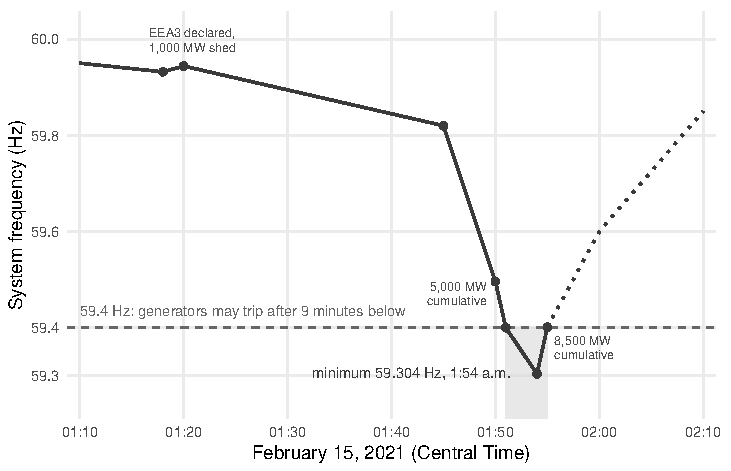
\includegraphics[width=\textwidth]{images/uri_frequency}
    \caption{ERCOT system frequency during the critical hour of February 15, 2021. Schematic: the line interpolates between values reported in the FERC/NERC staff report \autocite{FERCNERCFeb2021}; the recovery path after 1:55~a.m.\ is indicative. The frequency spent 4~minutes 23~seconds below the 59.4~Hz relay threshold.} % fig-src: analysis/figures/fig_ch2_uri_frequency.R
    \label{fig:frequency_drop}
\end{figure}

The human and economic impact was enormous. At the peak of the crisis about 4.5 million Texas homes and businesses were without power \autocite{CascadingRisks2021}, many for several days in freezing conditions. Tragically, the outage contributed to hundreds of deaths \autocite{DSHSWinterStormMortality2021}. The grid itself survived, thanks to those controlled outages. Over the following days (February 15--18), ERCOT worked to bring generation back and incrementally restore power. But until supply could meet demand again, utilities had to rotate outages to keep the reduced supply and high demand in balance.

\subsection{The 2003 Northeast Blackout}

On August 14, 2003, a sunny afternoon, a combination of technical glitches and human errors led to a cascading blackout across much of the Northeastern United States and Ontario, Canada. The trouble began when a series of FirstEnergy's high-voltage lines in northern Ohio tripped after contacting overgrown trees in their rights-of-way; the first was carrying well under half of its rated load, so this was a maintenance failure, not an overload \autocite{OutageTaskForce2004}. % src: Task Force Final Report pp. 17-19, 57-58: three 345-kV lines + one 138-kV faulted on tree contact; Harding-Chamberlin at 44% of rating; "overgrown trees, as opposed to excessive conductor sag"
Alone, those line losses would have been manageable. But FirstEnergy's control-room alarm system had silently failed almost an hour before the first line went down, so its operators did not know anything was wrong \autocite{OutageTaskForce2004}. % src: alarm and logging software failed 14:14 EDT; first tree contact 15:05 EDT; operators and IT support both unaware (pp. 51-53)
Power that had flowed on the failed lines shifted onto neighboring lines, which in turn overloaded and tripped in a chain reaction. Within minutes, a cascading failure was underway: as major transmission corridors went down, generators and loads across the region fell out of sync.

The disturbance rippled across the Northeast and parts of the Midwest and Canada, blacking out an estimated 50 million people and 61{,}800~MW of load in eight U.S. states and Ontario \autocite{OutageTaskForce2004}. % src: Task Force Final Report p. 1
In metropolitan areas like New York City, Cleveland, Detroit, and Toronto, power went out in a cascade that afternoon; parts of the United States waited four days for power, and parts of Ontario endured rolling blackouts for more than a week \autocite{OutageTaskForce2004}. The frequency in the affected areas plummeted as large power plants automatically shut down to protect themselves; in response, system protections began severing parts of the grid from each other to contain the collapse. The 2003 Northeast Blackout illustrated how interconnections meant to provide support can, under rare failure conditions, transmit disturbances far and wide. Its most lasting legacy was regulatory: the blackout led directly to mandatory, federally enforceable reliability standards for the North American bulk power system \autocite{OutageTaskForce2004,EPAct2005}. % src: Task Force Recommendation 1 (p. 140); EPAct 2005 sec. 1211 created FPA sec. 215; NERC certified as ERO 2006, standards mandatory June 2007

In Texas in 2021, supply crashed below demand; in the Northeast in 2003, uncontrolled power flows and losses caused parts of the Eastern Interconnection to fall out of sync. In each case, the grid's last-resort safety nets (automatic relays and operator-ordered outages) kicked in to try to stop the problem, but not before many customers were left in the dark.

\subsection{Why Recovery Takes Days or Weeks}

Once a grid has collapsed, why does it take days or even weeks to turn everything back on?

The core problem is that a power plant needs electricity before it can produce electricity. Fuel pumps, control systems, cooling equipment: all of it runs on station power that normally comes from the grid itself. When the grid is dead, most plants cannot start at all. Restoring a collapsed system therefore begins with a handful of designated \glossaryterm{black-start}{black start} units, typically hydroelectric plants or gas turbines with their own on-site generators, that can start with no outside power \autocite{NERCEOP005}. % src: NERC EOP-005-3, System Restoration from Blackstart Resources
Operators use them to energize pre-planned ``cranking paths'': transmission corridors that carry station power to larger plants, which then start up, pick up a small block of customers, and extend the electrified island outward \autocite{NERCEOP005}.

The balance rule from earlier in this chapter applies at every step. Each block of reconnected customers must be matched by generation already running, and a reconnected block briefly draws more than its normal share, because every thermostat and compressor in a cold, dark city switches on at once (operators call this cold-load pickup). Reconnect too much at once and the frequency of the young island collapses again, undoing hours of work. Separate islands must also be matched in frequency and voltage before they can be joined. Rebuilding a large grid is a sequence of thousands of careful, largely manual steps, which is why ERCOT's leadership estimated that a full black start of the Texas grid in 2021 would have left most of the state dark for weeks \autocite{MagnessTestimony2021,Douglas2021Seconds}. % src: Magness written House testimony (power out for 90% of Texans for weeks); Texas Tribune, Feb 18, 2021


\section{How Bitcoin Mining Can Support Grid Stability}

For the grid, Bitcoin mining is a highly \glossaryterm{flexible-load}{flexible} and controllable load: miners can rapidly scale down or shut off their power usage when needed. This flexibility means that, under the right incentives, Bitcoin miners can act as a kind of \glossaryterm{demand-side-reserve}{demand-side reserve} for the grid, helping balance supply and demand and prevent blackouts.

During normal times, miners operate around the clock, using electricity (often wherever it's cheapest or most abundant). But during grid stress events, say a hot summer afternoon when air conditioning load is at its peak or an unexpected power plant outage, miners can stop within minutes, freeing up electricity capacity to serve other critical needs. The industry calls this \glossaryterm{curtailment}{curtailment}, whoever sets it off: the site reading a price, or ERCOT or a generator sending an instruction the site has agreed to follow. Where it matters which of those happened, this book says \glossaryterm{pause}{pause} for the machine's own act. Nothing flows back into the grid when a mine stops; the generation it was using is simply free for everyone else, which has the same balancing effect as adding supply. A concrete example occurred in Texas in July 2022. Faced with record-breaking heat and electricity demand, over 95~percent of industrial-scale Bitcoin mines in Texas voluntarily paused during peak hours, freeing more than 1,000~MW of generation for other customers, according to the Texas Blockchain Council \autocite{TexasTribuneCrypto2022}. % src: TBC president Lee Bratcher, quoted in Chiu (Washington Post via Texas Tribune, Jul 15, 2022); industry self-report, not ERCOT-verified; Bratcher's own words were "push over 1,000 [megawatts] back into the grid", not repeated in prose because a load that stops injects nothing (glossary, load)
The council estimated that Texas miners curtailed more than 50,000~MWh over the month \autocite{UtilityDiveBitcoin2022}. % src: TBC statement reported by Utility Dive, Oct 19, 2022
That 1,000~MW was about 1.3~percent of ERCOT's heaviest demand hour that summer, enough to help the grid through the tightest hours without more severe emergency measures. The heaviest hour came on July 20, 2022, when demand across the grid averaged about 79,800~MW \autocite{EIAErcotPeak2023}. % src: EIA Today in Energy, Jul 26, 2023 (todayinenergy id=57240): "Previously, ERCOT's record for hourly demand was 79,830 megawatthours (MWh) on July 20, 2022." Chart note on the same page: hourly values "may differ from an instantaneous peak in demand", so MWh delivered in one clock hour = average MW sustained across that hour, which is why the prose says averaged and not peaked; 1,000/79,830 = 1.25%. Window is deliberately "that summer", not "on record": id=57240 shows 79,830 broken repeatedly in Jun-Jul 2023 (82,579 MWh on Jul 18, 2023), and EIA id=67906 (Jul 2026) gives 85.5 GW on Aug 10, 2023 and 91.1 GW on Jul 22, 2026

Winter tells the same story. In January 2024, Winter Storm Heather pushed ERCOT to five all-time winter demand records in four days, peaking at 78,349~MW on the morning of January 16 \autocite{ERCOTPeakRecords2024}, while the cold forced roughly 3,000~MW of additional generation outages \autocite{ERCOTMonthlyJan2024}. % src: 78,349 MW is the settled figure on ERCOT's 2024 Peak Demand Records page, unasterisked (ERCOT asterisks records pending settlement); the Jan-2024 Monthly prints 78,138 MW and labels its recap preliminary, so it carries the outages only; prior record 74,525 MW (Elliott, Dec 2022); Heather's record was itself surpassed by Winter Storm Kingston, Feb 20, 2025 (80,560 MW official)
ERCOT issued two conservation appeals and credited demand reductions, including by large flexible customers, with helping it avoid emergency operations \autocite{ERCOTConservation2024}. Bitcoin miners were a visible part of that response: network hashrate fell by roughly a quarter as Texas fleets paused \autocite{Hunt2024Hashrate}, and Riot Platforms alone earned \$3.3~million in curtailment and demand-response credits that month \autocite{Riot2024Jan}.
By the Texas Blockchain Council's own reckoning, wholesale prices during Heather's worst three days averaged only about \$100 per megawatt-hour, so much of Heather's curtailment was a response to prices, as Part~III examines in detail \autocite{Bratcher2024Data}. % src: Bratcher2024Data (TBC blog, Lee Bratcher, Jan 26 2024; verified at origin 2026-09-14): "The average settlement price of power on the wholesale market in ERCOT during the worst three days of the storm was $100.76 per MWh"; industry advocacy, affiliation now named in prose per source rule 4. TBC does not say which three days, so the window stays unnamed here per rule 5. Cross-check kept out of prose because the window is ours, not the monitor's: potomac2024som Table 8, p. 73 gives daily average RT prices across ERCOT's official Heather window of Jan 13-17 ($3.66, $70.78, $88.02, $148.71, $27.49); the mean of Jan 14-16 is $102.50 but Jan 15-17 is $88.07, so the agreement is window-dependent and the SOM never mentions Heather. Do NOT print TBC's companion claim that prices "never went over $600 per MWh": ERCOT Monthly Jan 2024 p. 4 shows a day-ahead price of about $1,900/MWh at the Jan 16 morning interval and System Lambda of about $1,134/MWh at the Jan 16 evening interval
Miners curtailed again during two winter storms in January 2025, mostly on price: Riot booked \$3.6~million in company-wide power credits for the month, of which \$3.2~million was curtailment and \$0.4~million came from formal ERCOT and MISO demand response programs, against \$1.0~million in December \autocite{Riot2025Jan}. The release does not split those demand-response credits between the markets. ERCOT called for no conservation during either storm and reported adequate supply to meet all demand \autocite{ERCOTMonthlyJan2025}. The flexibility works when the grid is merely strained, not only when it is breaking. % src: Riot Jan-2025 release (Feb 4, 2025) table: Power Credits $3.2M (fn 5, "Estimated power curtailment credits") vs $0.8M Dec-2024; Demand Response Credits $0.4M (fn 6, ERCOT and MISO programs); Total Power Credits $3.6M vs $1.0M Dec-2024 and $3.3M Jan-2024, so the $3.6M here is the same series as the $3.3M cited above for Jan 2024. ERCOT Monthly Jan 2025 (Feb 6, 2025) p.3 "January Winter Storms Recap": "The grid operated reliably during both winter storms with adequate supply to meet all demand"; "there was not a need to call for conservation and no outages were due to grid-wide reliability issues". Storms Cora (instantaneous peak 68,615 MW) and Enzo (77,758 MW). Do NOT restore "no grid emergency at all": same page records a transmission emergency in South and Southeast Texas, 5 a.m. to 1 p.m. Jan 21, about 29 iced lines, no controlled outages. The old comment's quote "less severe than recent historical winter storms" is not in that report and was dropped. Luxor cite removed earlier; Luxor banned as a source by the author, 2026-08-22

In January 2026, Winter Storm Fern brought another large response from flexible loads. The storm froze two-thirds of the country, and ERCOT's post-storm analysis estimated that underlying demand on the worst morning reached 84,558~MW, far past the all-time winter record and about 9,000~MW above what the meters actually recorded; the grid came through with no emergency alert, no conservation appeal, and no load shed \autocite{ERCOTMonthlyJan2026}. % src: ERCOT Monthly Jan 2026 (Feb 13, 2026), read at origin September 15, 2026: "the adjusted Monday morning peak was estimated at 84,558 MW" when the listed reductions are added back; those reductions sum to about 8,965 MW, hence "about 9,000 MW". The report gives NO metered peak; an earlier draft printed 75,572 MW, which appears in no ERCOT document and does not reconcile with the report's own arithmetic. Standing winter record 80,560 MW (Winter Storm Kingston, Feb 20, 2025, ERCOT records page); DOE issued a precautionary FPA 202(c) order Jan 24-27 that ERCOT never needed to invoke
The difference was flexible load stepping aside, and ERCOT itself did the accounting: roughly 4,100~MW of the reduction came from cryptocurrency miners, second only to the oil and gas sector and ahead of every other industry ERCOT counted, and more than twenty times what conventional data centers contributed \autocite{ERCOTMonthlyJan2026}. % src: same report: ~4,200 MW oil & gas, ~4,100 MW crypto, 420 MW steel, 170 MW data centers, 75 MW hydrogen/electrofuels; 4,100/170 = 24x
The response was visible in the Bitcoin network itself: roughly 200~EH/s went offline at U.S.-facing mining pools, average block times stretched to about 12.4 minutes against the protocol's 10-minute target, and the next difficulty adjustment was the largest downward move since China's 2021 mining ban. The adjustment after it more than made up the loss, up 14.7~percent, to about 2~percent above its level before the storm, as the machines returned \autocite{TheBlockFern2026,TheBlockDifficulty2026,BraiinsInsights}. % src: 200 EH/s offline and average block times "climbing to roughly 12.4 minutes" (The Block, Jan 26, 2026; theblock.co 403s to automated clients, read at the Wayback capture of 2026-02-09, retrieved 2026-09-14). 12.4 min implies hashrate about 19% below the difficulty-implied level (10/12.4 = 0.81); the Braiins Insights 1y series (7-day means) agrees in direction, and a sustained 40% drop would instead give about 16.7-minute blocks. -11.16% Feb 7 (The Block; Braiins Insights: 141.67 -> 125.86 T); rebound +14.73% to 144.40 T ~Feb 19-21 (Braiins Insights 1y series, verified 2026-08-22). NOT a record: ATH was 149.30 T in early Dec 2025; the old "snapping back to a record" claim was Luxor-sourced and wrong; Luxor banned as a source (author, 2026-08-22). CUT 2026-09-14: the "40% / ~455 EH/s trough" was a day-scale CoinWarz estimate reaching the book via CryptoSlate (Radmilac2026Fern), implying a ~1,138 EH/s baseline no series the book uses reproduces, in an article whose pool chart is sourced to banned Hashrate Index; cut under book-sources rule 6, cite dropped, entry removed from references.bib. Do NOT print a Braiins Insights percentage for this dip: three separate pulls on 2026-09-14 returned Jan 31 = 866.4 / 876.0 / 877.9 EH/s, giving -16.8% / -16.4% / -15.8% from Jan 24, so the figure is not reproducible at the precision print requires; 141.67 -> 125.86 -> 144.40 T, 144.40 / 141.67 = 1.0193, so about 2 percent above the pre-storm level; until 2026-10-10 "clawed back most of the lost ground" (review comment)
ERCOT's board chairman publicly credited the voluntary reductions by miners and data centers \autocite{FermanMalik2026}.

Bitcoin mining is suited to this role because it is an interruptible load by design. Stopping mining operations for a few hours doesn't ruin any product or inconvenience residential customers; it simply delays hashing, which miners accept when they are compensated for it, or when power prices are high. Miners describe their flexible load as a ``demand-side battery'': it soaks up excess power when supply is abundant (for instance, at night when wind farms might otherwise be curtailed) and shuts off on short notice when the grid is strained. The analogy has a limit: a battery can send back what it stored, while a mine stores nothing and can only stop drawing. Large mining farms can participate in demand response programs, getting paid to reduce consumption during grid emergencies just as industrial factories have long done. ERCOT has confirmed that miners ``respond during grid events by rapidly reducing their electric use,'' including during Uri \autocite{UtilityDiveBitcoin2022}.

Bitcoin mining can help address grid challenges alongside energy storage, other flexible industrial loads, and fast-ramping generation. A grid operator can achieve the same balancing effect as adding supply by curtailing a batch of miners that has signed up for it. As grids add more variable renewable generation and reserve margins tighten, a large consumer that can vanish in minutes becomes increasingly valuable. How miners are actually paid for that flexibility, through energy prices, ancillary services, and demand response programs, is the subject of Part~III.

\chapter{ERCOT: The Energy-Only Grid}
\label{ch:ercot}

The previous chapter treated the grid as a machine. This chapter treats it as a market, and one market in particular: ERCOT, the Electric Reliability Council of Texas, where more Bitcoin mining load is connected than anywhere else in the world. Everything in Parts II and III of this book (breakeven prices, curtailment strategies, ancillary services, transmission charges) plays out inside the market rules described here.

\section{From Monopolies to Markets}

For most of the twentieth century, electricity in the United States was delivered by \glossaryterm{vertically-integrated-utility-monopoly}{vertically integrated utility monopolies}: in each region, a single company owned the power plants, the wires, and the relationship with every customer \autocite{EPAMarketStructure}. Regulators, not markets, set the prices. State Public Utility Commissions approved investments and granted the utility an allowed rate of return; consumers had no choice of supplier.

Starting in the 1990s, federal policy pried this model open. FERC Order No.\ 888 (1996) required utilities to open their transmission lines to third-party generators on non-discriminatory terms, and Order No.\ 2000 (1999) encouraged the voluntary formation of \glossaryterm{regional-transmission-organization}{Regional Transmission Organizations} (RTOs): neutral, non-profit operators that run the grid and administer wholesale markets across multi-state regions \autocite{ferc1996order888,ferc1999order2000}. % src: Order 888 issued Apr 24, 1996; Order 2000 issued Dec 20, 1999 (89 FERC 61,285); verified from FERC pages/order PDF
Generation became a competitive business. Independent power producers could build plants and sell into open markets, and in many states consumers gained the right to choose their retail supplier. Today roughly two-thirds of U.S. electricity consumers live in regions where the transmission system, and the wholesale market on top of it, is run by these \glossaryterm{independent-system-operator}{Independent System Operators} (ISOs) and RTOs \autocite{EPAMarketStructure}; % src: EPA page (updated Jul 2026): "About two-thirds of U.S. electricity consumers live in a region where transmission is managed by an ISO or RTO"
 the rest remain under traditional regulated monopolies. ISOs and RTOs own no generation and serve no retail customers themselves. They dispatch generators, operate the transmission system, and run the auctions where electricity is bought and sold, which keeps them neutral among the competitors whose power they move.

Seven such markets serve most U.S. electricity consumers \autocite{isorto2026home}. % src: isorto2026home ("Ten ISOs/RTOs serve two-thirds of electricity consumers in the United States"; the seven U.S. ones are CAISO, ERCOT, ISO-NE, MISO, NYISO, PJM and SPP); until 2026-10-12 this said "cover most of the country", which is not true by area (review suggestion)
This book concerns itself with exactly one of them.

\section{The Island Grid}

ERCOT operates the Texas Interconnection introduced in Chapter~2: one of the three synchronous grids in the continental United States, and by far the smallest. It serves about 90~percent of Texas electric load, more than 27 million customers \autocite{ercot2026factsheet}. % src: ERCOT Fact Sheet, Aug 2026: "more than 27 million Texas customers, representing about 90 percent of the state's electric load"
Its isolation is deliberate. Because its wires stay (almost) entirely inside Texas, ERCOT's wholesale market is exempt from FERC rate regulation (federal reliability standards still apply), an arrangement Texas has defended since the 1930s \autocite{ercot2025gridinsightsabout}. % src: ERCOT Grid Insights, Nov 2025: "exempt from wholesale regulation by FERC... subject to FERC oversight through NERC's Reliability Standards"
The connections that do exist are three DC ties and one variable-frequency transformer, about 1,220~MW in total: 820~MW toward the Eastern Interconnection and 400~MW toward Mexico, less than two percent of ERCOT's peak demand \autocite{ercot2025gridinsightsdcties}. % src: ERCOT Grid Insights, May 2025: SPP ties 820 MW (North 220 + East 600), Mexico 400 MW (Railroad 300 + Laredo VFT 100); 1,220/91,200 (ERCOT's all-time peak demand, July 22, 2026; see ch8 sec:fourcp-peaks) = 1.3%
Isolation limits outside support and gives Texas autonomy over its market design. Chapter~2 showed that limit during Winter Storm Uri. Texas restructured its market on its own terms with Senate Bill 7 (1999), opening retail choice from January 2002, and it can change its market design without federal proceedings \autocite{texas1999sb7}. % src: Tex. Util. Code sec. 39.102(a), enacted by S.B. 7, 76th Leg. (1999); full retail competition from Jan 1, 2002

For a large electricity consumer, ERCOT's isolation also means operating entirely inside ERCOT's pricing system and market rules, with ERCOT as the only grid operator.

\section{An Energy-Only Market}

Most U.S. markets pay generators twice: once for the energy they produce, and once, through a \glossaryterm{capacity-market}{capacity market}, for simply existing and promising to be available years into the future. ERCOT does not. It is an \glossaryterm{energy-only-market}{energy-only market}: a generator earns money by selling energy and ancillary services, and nothing else \autocite{ercot2025gridinsightsabout}. If those revenues do not justify building a power plant, the plant does not get built.

If generators must recover their investment from energy prices alone, then prices during scarcity must be allowed to rise very high; those few expensive hours are what pay for the capacity that sits idle the rest of the year. ERCOT's price cap, and the mechanism that pushes prices toward it, are covered in Section~\ref{sec:ordc}. The same design is what makes ERCOT interesting for flexible consumers: a market that must occasionally produce extreme prices to function pays handsomely for the ability to get out of the way.

\section{Two Markets, One Grid: Day-Ahead and Real-Time}
\label{sec:dam-rtm}

ERCOT prices energy in two coupled markets:

The \glossaryterm{day-ahead-market}{Day-Ahead Market (DAM)} is a voluntary but financially binding forward market. Every day, participants submit offers and bids for each hour of the following day; ERCOT clears the market by co-optimizing energy and ancillary services, and publishes the resulting hourly prices in the early afternoon, by 1:30~p.m.\ Central Time \autocite{ercot2026dam,ercot2026protocols}. % src: ERCOT DAM page + WM201 deck: clearing starts 10:00 a.m., awards communicated by 1:30 p.m.; operationally 19:30 UTC in the tooling miners use (Braiins Academy timing table)
From that moment, tomorrow's day-ahead prices are public knowledge for every settlement point, whether or not a given consumer transacted. Publishing them does \emph{not} fix everyone's bill. A load pays the day-ahead price only for the volumes it actually bought in the DAM; whatever it consumes above or below that position settles at the real-time price \autocite{ercot2026protocols}. % src: Nodal Protocols sec. 4.6.2.2 (Day-Ahead Energy Charge applies only to cleared DAM Energy Bids) + sec. 6.6.3.2 (RT imbalance: day-ahead position vs Adjusted Metered Load settles at the RT price)

The \glossaryterm{real-time-market}{Real-Time Market (RTM)} balances the deviations. ERCOT runs its dispatch engine, called SCED (Security-Constrained Economic Dispatch), roughly every five minutes, repricing energy as actual conditions unfold, and since December 2025 ancillary services with it (Section~\ref{sec:rtcb}); settlement is on 15-minute intervals \autocite{ercot2026rtm,ercot2026protocols}. % src: ERCOT RTM page: SCED LMPs ~every 5 minutes, settlement point prices every 15 minutes (unchanged by RTC+B); ercot2026protocols sec. 2 (Real-Time Market: "A Real-Time, co-optimized market in the Operating Day for Ancillary Service capacity and energy"); RTC+B go-live December 5, 2025 (ercot2025rtcblive, sec:rtcb)
Real-time prices are far more volatile than day-ahead prices: a cloud bank over West Texas solar, a tripped generator, or an afternoon hotter than forecast shows up in real-time prices within minutes.

In practice, most large flexible loads, miners included, are exposed to that real-time price. The common supply structures are index contracts settled on the real-time zonal price, and fixed-price contracts that let the load resell unconsumed power at spot \autocite{potomac2024som}. % src: 2024 SOM: IMM documents large flexible loads practicing price response against real-time prices; Riot 10-K Rockdale fixed-price PPA with curtailment credits; IREN spot supply at Childress
And even a load that hedged every hour in the DAM makes its run-or-curtail decision against the real-time price, because curtailing frees the day-ahead energy it bought to be sold back at whatever real time pays. The afternoon prices are therefore a strong preview of tomorrow, not a locked-in bill: in 2024 the two markets differed by about \$17 per megawatt-hour on average in absolute terms \autocite{potomac2024som}. % src: 2024 SOM exec summary: DAM averaged $1.46/MWh above RT; mean absolute hourly difference $17.35/MWh, lowest since 2020
Chapter~6 lays out the full contract menu, from spot indexes to fixed-price contracts and standardized blocks, and builds the miner's curtailment strategy on exactly this structure.

The difference between the two prices at the same place and hour, the \glossaryterm{dart-spread}{DART spread}, is a market in itself: buy day-ahead and sell real-time, or the reverse. A consumer in ERCOT is always choosing, knowingly or not, between a price it can lock in this afternoon and a price that will not exist until the moment of consumption.

\section{Prices with an Address: Locational Pricing}

ERCOT does not have one electricity price; at any moment it has thousands. The unit of place in a power network is the bus, which the market calls a \glossaryterm{node}{node}: a physical junction where equipment connects to the high-voltage grid, such as the switchyard where a power plant's output feeds in, or a substation where transmission lines meet and transformers step the voltage down toward consumers. A node is a real place with coordinates; a large mine's own interconnection point is one. Roughly every five minutes, SCED computes a \glossaryterm{locational-marginal-price}{Locational Marginal Price} (LMP) at every node in its network model, the cost of delivering one more megawatt-hour at exactly that spot; the DAM computes the same thing once a day, for each hour of the next operating day: % src: until 2026-10-10 "once per hour", which read as an hourly rerun (review comment); the DAM clears once a day with a price for each hour of the next operating day (Chapter 3's Day-Ahead Market paragraph)
\[
\text{LMP} = \text{System Lambda} + \text{Congestion Cost}
\]
The first term, the \glossaryterm{system-lambda}{System Lambda}, is the cost of the next megawatt-hour anywhere on the system; the second is what the transmission limits between that node and the rest of the grid add or subtract. % src: ercot2026protocols sec. 2 (LMP: "offer and/or bid-based marginal cost of serving the next increment of Load at an Electrical Bus," produced by DAM or SCED); sec. 6.5.7.3 and sec. 6.5.9 (SCED produces Shadow Prices, System Lambda and LMPs; ERCOT distributes by ICCP and posts "System Lambda and the LMPs for each Resource Node, Load Zone and Hub"). Section 6 of the protocols uses System Lambda throughout and never the phrase System Energy Price, verified at origin September 15, 2026; the book uses System Lambda everywhere for that reason
When transmission is uncongested, prices across the system are nearly uniform. When a line reaches its limit, the grid splits into cheap and expensive regions, and the LMPs say so. Readers who know other U.S. markets will miss a third term. Every megawatt-hour loses a few percent of itself as heat on the way from plant to load, and PJM, MISO, and the other nodal markets price that loss into the LMP, so a node far from generation pays a little more for the extra energy that must be generated to reach it. ERCOT does not: its LMP has only the two components above, and transmission and distribution losses are recovered instead by scaling every load's metered consumption up by a loss factor before it is settled. The \glossaryterm{market-monitor}{market monitor} is the independent firm that \glossaryterm{the-commission}{the commission}, meaning the Public Utility Commission of Texas, selects to watch ERCOT for market power and design flaws. The monitor recommended marginal-loss pricing, but in early 2019 the commission declined to adopt it, judging the gain not worth the cost and disruption, and in 2020 the monitor retired its recommendation \autocite{ercot2026protocols,potomac2019som}. % src: potomac2019som p. xvii, PDF p. 25, "Retirement of Previous Recommendations" ("In early 2019, the Commission declined to direct ERCOT to implement marginal losses in ERCOT locational marginal prices"; the Commission "concluded that the incremental benefit of applying marginal losses in the ERCOT market is not worth the implementation cost and market disruption"; hence the IMM retiring the recommendation; the report is dated May 2020; reordered 2026-10-12 after a review comment that the commission, not the monitor, shelved the idea); ercot2026protocols sec. 2 (Transmission Loss Factor: "the fraction of ERCOT Load ... that is considered to constitute the ERCOT Transmission Grid losses in a Settlement Interval"; Distribution Loss Factor; Unaccounted for Energy) and sec. 13 (Transmission and Distribution Losses)
For a miner the practical consequence is small but real: where the site sits in the network changes its price only through congestion, not through distance from the plants.

Nobody is billed on raw bus prices, though. Money changes hands at \glossaryterm{settlement-point}{settlement points}, at prices built from the LMPs over each 15-minute settlement interval \autocite{ercot2026protocols}. % src: Nodal Protocols sec. 6.6.1 (RT SPPs: resource node = time-weighted avg of SCED LMPs, incl. reliability-deployment adder, floor -$251/MWh; load zone = load-weighted avg of zone bus LMPs; hub = simple avg over hub buses per sec. 3.5.2); DAM SPPs hourly per sec. 4.6.1
A generator is paid the time-weighted average of the five-minute LMPs at its own bus, its \glossaryterm{resource-node}{resource node}. A consumer pays its \glossaryterm{load-zone}{load zone} price: an average over every bus in the zone, weighted by how much load each bus is carrying. ERCOT defines eight zones: the four large competitive zones mapped in Figure~\ref{fig:lz-map}, and four smaller ones belonging to utilities that did not open to retail competition (Austin Energy, CPS Energy, LCRA, and Rayburn). Traders hedge at \glossaryterm{hub}{hubs} (North, South, West, Houston, and a few others), whose prices average the LMPs of fixed lists of major 345~kV buses and anchor most financial contracts. % src: hub count fix per Protocols sec. 3.5.2: five in-force geographic hubs (incl. Panhandle) plus Hub Average and Bus Average; LRGV hub gray-boxed, hence "and a few others", no hard count
The price at a power plant's fence line, the price on a miner's invoice, and the price a futures contract settles against are three different aggregations of the same underlying five-minute prices.

There is one exception: ERCOT settles what it dispatches at the node itself. A grid battery's charging energy already settles at its resource node rather than the zone, and a 2024 rule change, approved and scheduled for early 2027, will extend nodal dispatch and settlement to \glossaryterm{controllable-load-resource}{Controllable Load Resources}: loads that give ERCOT's dispatch engine direct control in exchange for fuller market participation, a registration some miners hold. A Controllable Load Resource that aggregates small sites, each under 10~MW, stays zonal \autocite{ercot2024nprr1188,potomac2026somercot}. % src: NPRR1188 PUCT-approved Nov 21, 2024, gray-boxed "upon system implementation" in the Aug 2026 Protocols: ercot2026protocols sec. 3.6.1(5) (a CLR that is not an ALR settles at "its Resource Node Settlement Point", an ALR at "its Load Zone Settlement Point") and sec. 2 (ALR: "an aggregation of individual metered sites, each of which has less than ten MW of Demand response capability and all of which are located within a single Load Zone"); ercot2024nprr1188 description (CLRs that are not ALRs "are dispatched at a nodal shift factor and settled for their energy consumption at a nodal price"); schedule: potomac2026somercot p. 45 ("scheduled for completion in early 2027") and p. 30 n. 14 (January 2027, per ERCOT project management), as chapter 7 sec:as-catch prints; ERCOT's project list of Sept 24, 2026 (Revision_Requests_2026_09_24.xlsx: project 539-01, NPRR1188 and NPRR1244, Execution, target end March 1, 2027; January 1, 2027 and Planning in the April 14 list); ESR charging nodal + excluded from zonal AML per Protocols sec. 6.6.3.2
Until that switches on, every consumer's energy, controllable or not, is billed at the zonal price.

\begin{figure}[h]
  \centering
  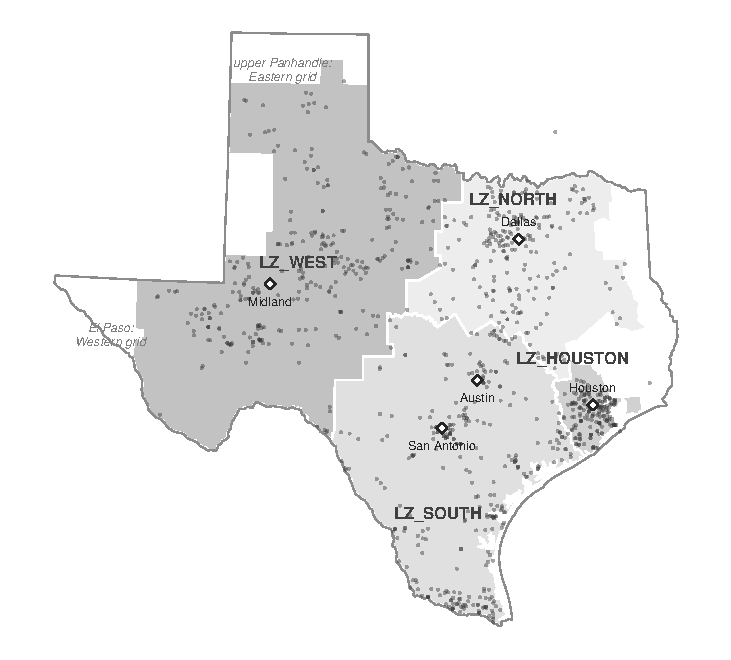
\includegraphics[width=\textwidth]{images/ercot_lz_map}
  \caption{
    ERCOT's four competitive load zones, with generation-side nodes approximated by the 988 grid-connected power plants (dots). The four smaller load zones of the utilities that did not open to retail competition are non-contiguous enclaves within these areas and are not drawn; zone boundaries are approximate, because ERCOT defines zones as sets of electrical buses, not geographic borders. White areas of Texas lie on the Eastern and Western Interconnections, outside ERCOT. Data: EIA-860M, June 2026 \autocite{eia860m2026}. % fig-src: analysis/figures/fig_ch3_lz_map.R (zones: derived third-party GIS tracing of ERCOT's published map, unlicensed re-host, hence "approximate"; outline: Census cb_2023_us_state_20m; plants: EIA-860M BA=ERCO; node/bus coordinates are not published by ERCOT)
  }
  \label{fig:lz-map}
\end{figure}

One of those load zones, \glossaryterm{lz-west}{LZ\_WEST}, appears throughout this book. West Texas has the state's best wind and solar resources, limited transmission out, and, not coincidentally, much of its Bitcoin mining. The result is the most volatile prices in ERCOT: hours of cheap or even negative prices when renewable output exceeds what the wires can carry away, and violent spikes when it does not. During hours with negative prices, generators pay consumers to take power, because subsidized renewables can profitably produce below zero and shutting down costs them more. Chapter~6 quantifies how often.

\section{Scarcity Pricing and the \texorpdfstring{\$5,000}{USD 5,000} Cap}
\label{sec:ordc}

An energy-only market needs administered scarcity pricing, because operating reserves, the safety margin Chapter~2 described, are valuable even in hours when no shortage materializes. From 2014 until the 2025 market redesign, ERCOT implemented this through the \glossaryterm{operating-reserve-demand-curve}{Operating Reserve Demand Curve} (ORDC): a real-time adder to the energy price that grows as available reserves shrink, reflecting the rising probability of losing load \autocite{puct25509}. % src: scarcity pricing mechanism now codified at 16 TAC 25.509; ORDC implemented June 2014 (LOLP x VOLL; VOLL $9,000/MWh in 2021 per potomac2021som p. vi, "the VOLL and HCAP of $9,000"; now set to the HCAP for DAM, $5,000, per ercot2026protocols sec. 4.4.11(1)(a)); under RTC+B the ORDC adder was absorbed into ancillary-service demand curves (see sec:rtcb)
When reserves were plentiful the adder was near zero. When reserves ran thin, the adder pushed prices toward the \glossaryterm{system-wide-offer-cap}{system-wide offer cap}: \$5,000 per megawatt-hour, lowered from \$9,000 after Winter Storm Uri \autocite{ercot2021hcapnotice,puct25509}. Since the redesign of Section~\ref{sec:rtcb}, the ancillary-service demand curves do that pushing from inside the energy price \autocite{ercot2026protocols}. % src: PUCT approved Dec 2, 2021, effective Jan 1, 2022 (ERCOT market notice M-A120721-01); HCAP $5,000 / LCAP $2,000 per 16 TAC 25.509 (b)(6)(A)-(B); still $5,000 as of Aug 2026; since RTC+B ercot2026protocols sec. 4.4.11(1)(a) sets the VOLL used to build the ASDCs to the HCAP for DAM and sec. 6.5.7.3(14)(d) caps bus LMPs, System Lambda and the Real-Time MCPCs at that effective VOLL; real-time energy offers themselves stop at the RTSWCAP, $2,000 (sec. 4.4.11(1) parameter table; sec. 4.4.11(2) rejects offers above it), not printed
A second, smaller adder has ridden on top of it since June 2015, the reliability deployment price adder. When ERCOT keeps the lights on outside the market, by ordering extra generators online or calling on demand response, it adds supply or removes demand and so pushes the price down just when the grid is short; the adder reruns the dispatch as if those actions had not happened and puts the difference back into the price. On average it is small: in 2025 it added \$0.41 per megawatt-hour to the price of energy, against \$0.02 for the ORDC adder. Unlike the ORDC adder, it survived the redesign of Section~\ref{sec:rtcb} \autocite{potomac2015som,potomac2026somercot}. % src: potomac2015som p. 2 (the reliability adder "was implemented on June 25, 2015"; NPRR626 per p. xxv); potomac2026somercot p. 8 ("Actions such as Reliability Unit Commitments (RUCs) and deployment of ERS demand response can artificially lower prices by increasing supply or reducing demand outside the normal market process. The RDPA corrects this suppression by increasing real-time prices when these actions occur"), p. 3 note 2 ("uses the dispatch software to simulate the system lambda without RUCs, deployed load capacity, or certain other reliability actions"), p. 1 ("the ORDC and the RDPA added $0.02 per MWh and $0.41 per MWh, respectively, to the price of energy"; also p. 9), p. A-10 (the RDPA "remains after RTC is implemented", now with separate adders for energy and each AS product); added 2026-10-12 after a review comment that Chapters 5 and 6 and the glossary refer back to an adder this section never introduced

In 2025, a typical ERCOT hour cleared somewhere between \$20 and \$40 per megawatt-hour (the middle half of the year's real-time hours, all eight load zones pooled). % src: analysis/checks/ch3_typical_hour.R console: real-time market, ERCOT MIS 13061 15-min settlement point prices (analysis/data/ercot_rtm15_spp_loadzones_2021on.csv.gz) averaged to clock hours, all eight load zones pooled, calendar 2025: middle half of hours $20.29 to $39.81, median $26.56; holds in 2025; the 2026 partial year comes close ($18.12-$34.83); not in every year: 2024 ran $14.19-$27.74 and 2022 $28.92-$67.43; LZ_WEST alone ran $20.16-$56.74 in 2025
The cap is more than a hundred times that. Prices near the cap arrive rarely, a handful of hours in most years, but for a consumer those hours are catastrophic to buy through and lucrative to avoid. Much of the economic case for miner flexibility in Part III rests on this asymmetry.

Two mechanisms can lower that cap. Since December 2023 the \glossaryterm{emergency-pricing-program}{Emergency Pricing Program} cuts it to \$2,000, for energy and ancillary services alike, once real-time prices have been at \$5,000 for 12 hours within any 24, and holds it there for at least a day and until a day after any emergency ends. And once a hypothetical new peaking plant's earnings above fuel pass \$315,000 per megawatt in a calendar year (three times its yearly building cost), the cap falls to \$2,000 for the rest of that year. Only Uri ever crossed that line, and the commission held off the drop until March 3, 2021, because the low cap then in force was pegged to gas prices and would have come out above \$9,000 \autocite{puct25509,ercot2026protocols,potomac2026somercot,potomac2021som}. % src: puct25509 (c)(1) (EPP "must be activated if the system-wide energy price, as determined by ERCOT, has been at the HCAP for 12 hours within a rolling 24-hour period"), (c)(2) (ECAP = LCAP "for both energy and ancillary service offers"), (c)(3) (in effect until the later of 24 hours after activation or, if ERCOT entered or stayed in emergency operations, 24 hours after it exits them), (b)(2), (b)(4) and (b)(6)(C)-(D) (peaker net margin: RTEP less 10 x the gas index, summed where positive; HCAP "until the peaker net margin during a calendar year exceeds a threshold of three times the cost of new entry", then LCAP "for the remainder of that calendar year"); the EPP is the (c) that PUCT Project 54585 added, effective December 20, 2023 (adoption order: it implements SB 3 sec. 18 "by establishing an emergency pricing program (EPP)"); ercot2026protocols sec. 4.4.11(1)(a)(i) (the trigger is RTM System Lambda plus the Real-Time Reliability Deployment Price Adder for Energy at or above the HCAP for DAM for 12 hours in a rolling 24, on SCED data time-weighted to 15-minute intervals), (1)(a)(ii) and (f), the parameter table (ECAP $2,000, LCAP $2,000, PNM threshold $315,000 per MW-year) and sec. 4.4.11.1(3); potomac2026somercot p. 103 ("three times the CONE over a calendar year, or $315 per kW-year"; "exceeded only once in ERCOT's history, on February 16, 2021, during Winter Storm Uri"); potomac2021som pp. v-vi (the LCAP then "the greater of either $2,000 per MWh or 50 times the natural gas price", which "exceeded the HCAP of $9,000", so the Commission suspended it) and pp. 11-12 and 95 (the suspension "was terminated on March 3, 2021" and the Commission directed ERCOT to resume the LCAP, Project 51812 order of that date); pp. vi and 94-95 say the suspension "occurred" on March 3 and that the Commission "suspended use of the LCAP on March 3"; the date is the reinstatement, per footnote 89 (Project 51812, Order Reinstating Low System-Wide Offer Cap, Mar. 3, 2021) and pp. 11-12
So under the rules in force in 2026 the week of Chapter~2 could not recur at its price, and every value this book measures in that week, in Chapters~6, 7 and~9, was priced under 2021's rules \autocite{puct25509}. % src: puct25509 (c)(1)-(3) (EPP trigger and duration) and (d) ("Beginning January 1, 2026, and every five years thereafter, the commission will review each of the system-wide offer cap programs"); ercot2026protocols sec. 6.5.7.3.1(2)(o) (during ERCOT-directed firm load shed in EEA Level 3 the reliability deployment adder lifts the price to the VOLL used for the RTM ASDCs, which sec. 4.4.11(1)(a)(i) sets to the ECAP while the EPP is active); Uri week at $9,000 for days: chapter 6 sec:indexbill (oxner2021paxtongriddy); the values measured in that week: chapter 6 sec:ownergen (sell option), chapter 7 section "What Standing By Paid" (2021 AS prices), chapter 9 sec:stack-sum and sec:stack-fence (the 2021 ledger year)

\section{Ancillary Services: A First Look}
\label{sec:as-overview}

Alongside energy, ERCOT buys \glossaryterm{ancillary-service}{ancillary services}: standing capabilities that keep the lights on when something breaks. Chapter~2 explained why frequency must be defended second by second; these are the products that defend it. ERCOT's current set has five members \autocite{ercot2025astopics}: % src: ERCOT Trending Topics: Ancillary Services (Dec 2025): Reg-Up, Reg-Down, RRS, ECRS, Non-Spin; ECRS go-live June 9-10, 2023

\begin{itemize}
  \item \glossaryterm{regulation}{Regulation Up and Regulation Down} (Reg-Up, Reg-Down): fast-ramping capacity under ERCOT's automatic control, adjusted on a four-second signal to smooth the continuous wobble between supply and demand.
  \item \glossaryterm{responsive-reserve-service}{Responsive Reserve Service} (RRS): the primary frequency-defense product, deployed automatically when frequency drops. Notably for this book, a large share can be provided by \glossaryterm{load-resource}{load resources}, consumers registered with ERCOT to sell ancillary services; the basic kind sells RRS by tripping offline within half a second on an under-frequency relay \autocite{ercot2026protocols,ercotnog2026}. A miner can hold this role: the ability to disconnect quickly is itself a sellable service. % src: ercot2026protocols sec. 2 (Load Resource: "A Load capable of providing Ancillary Service to the ERCOT System and/or energy in the form of Demand response and registered with ERCOT as a Load Resource"), sec. 3.6.1(1)(a)(iii) (RRS from a CLR with Primary Frequency Response or from a Load Resource on a high-set under-frequency relay) and sec. 3.16(4) (relay loads and FFR together at most 60% of the RRS requirement, the share chapter 7 sec:clr prints); ercotnog2026 sec. 2.3.1.2(6)(a) (total interruption within 30 cycles, 0.5 s, including relay and breaker)
  \item ERCOT Contingency Reserve Service (ECRS): capacity deployable within ten minutes after a contingency such as a large generator trip, introduced in June 2023. Chapter~9 examines the trade-off between selling ECRS and keeping the mine free to stop when electricity costs more than mining earns.
  \item \glossaryterm{non-spinning-reserve}{Non-Spinning Reserve} (Non-Spin): slower backup, capacity that can come online within thirty minutes.
\end{itemize}

What these products pay, and why those payments collapsed after 2021, is the subject of Chapter~7. ERCOT pays for readiness as well as energy, and in the market's eyes a load that can vanish in seconds is a form of readiness.

\section{Paying for the Wires: 4CP}
\label{sec:4cp-intro}

Energy prices do not pay for transmission lines. In ERCOT, transmission costs are allocated by a mechanism with outsized consequences for large consumers: \glossaryterm{4cp}{Four Coincident Peak}, or 4CP. For each summer month (June through September), ERCOT identifies the single 15-minute interval in which system-wide demand peaked. Demand here is a settlement quantity, not the raw load on the control-room screen: ERCOT sums the metered output of its generators, nets off the flows over the DC ties, and excludes the charging of grid-scale batteries entirely \autocite{ercot2026protocols}. % src: Nodal Protocols sec. 9.17.1 (4CP determination: generation-side balance, +DC-tie imports/-exports, +/-Block Load Transfers, minus Wholesale Storage Load); ERCOT notice M-B080124-01 warns the settlement 4CP interval can differ from the interval of highest observed demand; NPRR1188 gray boxes, upon system implementation (early 2027), not printed: sec. 9.17.1(3) (a joint NPRR995 and NPRR1188 box) and (4) also subtract the portion of non-ALR CLR load, and of non-WSL charging load, supplied by co-located generation at sites with a net metering arrangement; sec. 11.1.6(4), for a single-POI Generation Resource site that includes a CLR, counts only the CLR load supplied from the grid in 4-CP and LRS volumes ((c)) but settles the CLR's total load, grid-supplied plus co-located, for energy at the Resource Node ((d)); so a grid-supplied CLR's 4CP is unchanged, and a co-located CLR keeps the netting of any netted load for 4CP and LRS though not for energy (NPRR1188 ERCOT comments, April 4, 2024: co-located CLRs "should receive the same treatment as other types of co-located Load")
A large consumer's share of the following calendar year's transmission costs is then set by its average consumption during exactly those four intervals \autocite{puct25192}. % src: 16 TAC 25.192 (eff. Dec 20, 2022): 4CP data filed by Dec 1 bills transmission for the next year; TDU tariffs (e.g. Oncor) pass through to IDR-metered customers by the customer's own 4CP demand, fixed each Jan 1

Large consumers forecast when the peaks will occur and switch off for them. The metered exposure is one hour a year, four 15-minute intervals, but ERCOT confirms each interval only after the month ends, so in practice loads curtail longer windows across several candidate afternoons. Done well, that discipline can eliminate a transmission bill in the millions. Chapter~8 quantifies what 4CP avoidance is worth per megawatt and how miners chase it.

\section{Real-Time Co-optimization: The 2025 Redesign}
\label{sec:rtcb}

In December 2025, ERCOT switched on its largest redesign since nodal pricing: \glossaryterm{real-time-co-optimization-plus-batteries}{Real-Time Co-optimization plus Batteries} (RTC+B). Before it, ancillary services were bought once, in the Day-Ahead Market, and held fixed; energy was then dispatched around those fixed positions all day. After it, every five-minute SCED run procures energy \emph{and} ancillary services together, repricing both continuously; the old ORDC adder of Section~\ref{sec:ordc} is gone, absorbed into the energy price, and only its curve survives, as the shape the new ancillary-service demand curves are cut from \autocite{ercot2025rtcblive,potomac2026somercot}. % src: ERCOT news release Dec 5, 2025 (go-live); Trending Topics: AORDC used to build AS Demand Curves as inputs to DAM and SCED; ERCOT projects savings exceeding $1B annually. potomac2026somercot p. 2 ("the Operating Reserve Demand Curve (ORDC) Adder, implemented in 2014 and discontinued in December 2025 with the introduction of RTC"), p. 3 ("Since RTC was implemented, shortage pricing has been incorporated into the price of energy rather than functioning as a separate adder"), App. p. A-7 ("These ASDCs effectively replace the ORDC price adder"), App. G ("The ORDC price adder ... was replaced by a set of ASDCs"). The earlier "lives on" wording inverted this and was corrected 2026-09-20

For flexible loads this is a regime change: the value of standing ready is now marked to market every five minutes rather than locked in the afternoon before. The early evidence of what RTC+B does to ancillary prices appears in Chapter~7, and its implications for mining strategy in Chapter~10.

\section{Bitcoin Miners in the ERCOT Market}
\label{sec:miners-ercot}

Each miner deals with ERCOT through a \glossaryterm{qualified-scheduling-entity}{Qualified Scheduling Entity} (QSE). A mine's energy is settled through the QSE of whoever sells it power, and a mine that sells reserves registers as a load resource, whose QSE is a firm it hires or, once it qualifies, itself (Chapter~7) \autocite{ercot2026protocols}. % src: ercot2026protocols (Aug 1, 2026) sec. 16.3.1.1(1) (each LSE applicant "shall designate the Qualified Scheduling Entity (QSE) that will perform QSE functions per these Protocols on behalf of the LSE", with a written statement that the QSE "accepts responsibility for the applicant's transactions"); sec. 3.6.1(2) ("Except for voluntary Load response and ERS, loads participating in any ERCOT market must be registered as a Load Resource") and (3) ("All ERCOT Settlements resulting from Load Resource participation are made only with the Qualified Scheduling Entity (QSE) representing the Load Resource"); sec. 16.5.1.1(1) (each Resource Entity applicant "shall designate" its QSE) and sec. 16.2.3.2(1) ("a Resource Entity serving as its own QSE"), as chapter 6 sec:ownergen and chapter 8 sec:aggregators print
Any load of 75~MW or more at a single site must complete ERCOT's large-load interconnection process, with system studies and a separate approval to energize, before it may draw power \autocite{ercot2025nprr1234}. % src: NPRR1234 (board approved Apr 8, 2025; PUCT approved May 15, 2025; effective Jul 21 / Dec 15, 2025); grew out of the withdrawn NPRR1191
By the end of 2025 ERCOT's large-load program, which takes loads of every industry and not only miners, had about 5,800~MW energized, each site counted at the highest draw it has ever reached. By March 2026 over 9,000~MW, those sites included, held ERCOT's approval to energize \autocite{ercot2026llistatus}. % src: ercot2026llistatus slide 3 (5,768 MW Observed Energized in the 2025 column, defined as projects approved to energize and fully operational, "Represented by all time non-simultaneous peak load consumption"; all project types, with no split by industry anywhere in the deck; the 2025 column's approved total is 6,714 MW, 5,768 energized plus 946 approved but not operational), slide 4 (Approved to Energize by snapshot: 8,786 MW at 2025-12 and 2026-01, 9,042 MW from 2026-02, so the 9,000 MW is dated to the March 2026 deck, not to 2025), slide 5 (approved to energize 5,136 MW LZ_WEST + 3,907 MW other = 9,043 MW, each bar the observed peak plus the remaining approved load) and slide 6 (9,042 MW); the earlier "historically dominated by miners" had no support in the source and was dropped 2026-09-26 (ENERGY-009)
Mining demand alone, by the market monitor's count, peaked near 4,600~MW in 2025 (Chapter~7) \autocite{potomac2026somercot}. % src: potomac2026somercot p. i ("Aggregate demand for crypto-currency mining was approximately 4,600 MW in 2025"), p. 14 (4.6 GW), p. 31 ("peak demand reaching 4,600 MW in 2025"); a different count from the program total above, and neither contains the other: the monitor's figure is mining only, the program's is every industry at 75 MW or more
As Chapter~2 described, during Winter Storm Fern, ERCOT's own analysis credited about 4,100~MW of curtailment to cryptocurrency miners, second only to oil and gas and ahead of every other industry it counted \autocite{ERCOTMonthlyJan2026}. The queue behind them has changed character, though: of the roughly 410~GW of requests from prospective large loads ERCOT was tracking by early 2026, nearly 88~percent were AI data centers and less than 4~percent were mining, the interconnection-side echo of the pivot described in Chapter~1 \autocite{vegas2026senateupdate}. % src: ERCOT CEO Pablo Vegas, Texas Senate B&C testimony, Apr 1, 2026: 410,618 MW tracked by 2030; 87.6% data centers, 3.8% crypto

The rulebook also has words for how a mine sits relative to the grid, and several of them matter later in the book. A \glossaryterm{private-use-network}{Private Use Network} is, in ERCOT's own definition, ``an electric network connected to the ERCOT Transmission Grid that contains Load that is not directly metered by ERCOT (i.e., Load that is typically netted with internal generation)'': a mine built beside a power plant and metered together with it where the pair meets the grid, so that only the net flow is ever settled \autocite{ercot2026protocols}. % src: ercot2026protocols sec. 2 (Private Use Network, verbatim)
ERCOT's definitions also give the 75-megawatt load a name, \glossaryterm{large-load}{Large Load}; if half or more of its demand is ``computational load, such as data centers and cryptocurrency mining facilities,'' it is a \glossaryterm{large-computational-load}{Large Computational Load}, the term the commission's transmission reform in Chapter~8 asks about by name \autocite{ercot2026protocols}. % src: ercot2026protocols sec. 2 (Large Load; Large Computational Load, verbatim)

In 2026 ERCOT began studying its queue of large loads in one batch rather than one by one. In that study a network that pairs a plant with a large load could ask to be treated as a \glossaryterm{withdrawal-limited-private-use-network}{Withdrawal-Limited Private Use Network}: ERCOT models the plant switched off and fixes a hard cap on what the site may draw from the grid. The site may then build up to the plant's output on top of that cap, so a large load that brings its own generation can connect before the transmission upgrades for its full draw are built \autocite{ercot2026protocols,ercotplanningguide2026}. % src: ercot2026protocols sec. 2 (WLPUN: withdrawal limit determined by a system-wide interconnection study conducted by ERCOT) and sec. 3.10.7.3.1 (net Demand at the POI may not exceed the limit; one-minute cure); Planning Guide sec. 9.3.2 (PGRR145, effective July 11, 2026: WLPUN allocated peak Demand capped at the withdrawal limit plus the network's generation)
Chapter~6 prices what such a network is worth to a miner, and what it costs.
The same study offered a second elective route, this one to a large load that brings no plant. A load that asked to be studied as a \glossaryterm{provisional-controllable-load-resource}{Provisional Controllable Load Resource} may draw above the demand the study says the network can serve, up to its full request and with no guarantee that the grid can serve it in real time. It may do so only while it stays registered as a Controllable Load Resource taking ERCOT's dispatch, with its bids capped when a nearby constraint is at risk and no ancillary services to sell. The rules passed with the rest of the batch study in June 2026; the dispatch code behind them is a build ERCOT has ranked for 2027. The window to ask for either route closed in July 2026 \autocite{ercotplanningguide2026,ercot2026protocols}. % src: Planning Guide secs. 9.2.2.1(2) and 9.2.2.2(2) (Form W Part A and Form X due to the Interconnecting DSP or TSP "on or before July 10, 2026", which forwards them to ERCOT "on or before July 24, 2026") and sec. 9.3.1(2)(a) (all Large Load information due to ERCOT by July 24, 2026); Section 9 (effective July 11, 2026) defines only the Batch Zero and legacy procedures and refers to "a future interconnection study process" (sec. 9.2.1(4)) without defining one; Planning Guide secs. 9.2.2.1, 9.3.2 and 9.4.1 (PGRR145: election by Form W; maximum LPC set to the peak Demand that may be served reliably, requested peak Demand approved as MPC contingent on registration; PCLRs exempt from the minimum allocation threshold); Protocols sec. 2 (PCLR definition), sec. 23 Form W (no Real-Time guarantee; PCLRs not eligible to provide Ancillary Services), sec. 6.5.7.3 (dynamic capping of PCLR energy bid curves) and sec. 16.5.5 (de-registration returns the load to its LPC); PUCT approved June 18, 2026, PCLR sections effective upon ERCOT system implementation, priority 2027
In August, at the governor's direction, ERCOT held the study's final verdicts back for an audit of every load's eligibility, due in December. Until that audit and a review of community impact are done, it has stopped approving new data centers and mining sites of 75~MW or more to energize \autocite{ercot2026batchzero}. % src: ercot2026batchzero slides 1 and 3-4 (Governor Abbott's directive of August 3, 2026, a letter per ERCOT market notice M-A080326-01 of the same day; ERCOT's notice paused the Batch Zero study process and delayed final classification, which is now due in December with the Eligibility Verification Report of December 10, 2026, originally August 7, 2026; conditional classification still went to the TSPs on September 3, 2026, as chapter 10 sec:outlook-grid prints; approvals to energize data centers and virtual currency mining facilities of 75 MW or greater paused until the verification and audit and the community impact review, whose report is also due December 10, are complete; impact on the study timeline "TBD", originally April 9, 2027 under Planning Guide sec. 9.3.1(2)(b))

The market rules of this chapter explain \emph{why} Texas, and West Texas in particular, accumulated so much Bitcoin mining. Published day-ahead prices make tomorrow's expensive hours visible in advance. Locational pricing hands the cheapest, most volatile prices to the region with the most stranded renewable energy. Scarcity pricing makes the worst hours expensive enough that avoiding them is a business. Ancillary services pay for interruptibility itself, and a load that disappears for four well-chosen quarter-hours a summer walks away from its share of the transmission bill. In August 2023, a record month, Riot Platforms booked \$24.2~million for reselling at spot the power its fixed-price contracts had bought and \$7.4~million from ERCOT's demand-response programs, while the 333 bitcoin it mined were worth roughly \$9.5~million; on the real-time index the same pauses would have bought no power and booked no resale credit (Chapter~6) \autocite{riot2023august,riot10k2024}. % src: Riot press release Sep 6, 2023 (SEC 8-K Ex. 99.1; release and table re-read 2026-09-27): "a new monthly record for Power and Demand Response Credits, totaling $31.7 million in August" (the two components are printed, not the total, which the release rounds: 24.2 + 7.4 = 31.6); table: Power Credits $24.2M, fn "Power curtailment credits received from the Company's ability, under its long-term power contracts, to sell power back to the ERCOT grid at market-driven spot prices"; Demand Response Credits $7.4M, fn "Credits received from participation in ERCOT demand response programs"; "Power Credits and Demand Response Credits for July and August 2023 are estimates"; 333 BTC produced, 300 sold for $8.6M net at $28,617 average net price -> 333 x 28,617 = $9.53M (at the August average price implied by Riot's "approximately 1,136 Bitcoin" equivalence, 31.7M / 1,136 = $27,905, $9.29M); the credits are gross, counted before the bitcoin the curtailed hours would have mined, which no public source gives, so no net figure is printed; the old "the flexibility paid more than three times the mining" (31.7 / 9.53 = 3.3x) was retired 2026-09-27 (EXEC-021) because it read as a net payoff; riot10k2024 Note 20 (Rockdale PPA: 345 MW of long-term, fixed-price power, with the election not to use it and to sell it instead, as the opening of chapter 6 prints); index equivalence: chapter 6 sec:arbitrage ("the contract price cancels out of the decision") and chapter 9 sec:stack-contract (S19j Pro pause option $1.41M on the real-time index and $1.41M under a fixed $27 contract with sell-back, 2025); each resold MWh is credited P - F, the price less the fixed price, which is (P - V) + (V - F), and only the option P - V is index-equivalent, the V - F being the margin mining would have earned anyway (chapter-6.tex sec:arbitrage, the Riot credits sentence, riot10k2024: "the difference in the market power price and our fixed power price"), so on the index the same pauses are worth less than the $24.2M; the $7.4M of demand-response credits is paid the same on either contract; until 2026-09-27 this line said the resale was "worth the same" on the index, and the clause saying so is gone

Miners can earn money through ERCOT's incentives for flexible consumption without anyone needing to believe in bitcoin. How much that flexibility earns, hour by hour and program by program, is the business of the rest of this book.


\part{The Economics of Mining as a Load}

\chapter{Mining Economics: Hashprice, Efficiency, Breakeven}
\chaptermark{Mining Economics}
\label{ch:economics}

Part I ended with a market that pays loads to be flexible. Before this book can price that flexibility, it has to answer a more basic question: what does a mining machine actually earn, what does it spend, and where exactly is zero? Chapter~1 promised the full derivation of the breakeven arithmetic; this chapter delivers it, and everything after runs on it. One formula connects the mining industry's unit system (dollars per terahash-day) to the energy industry's (dollars per megawatt-hour). Once you can move between those two currencies, curtailment strategies, strike prices, and ancillary-service bids all become readable.

\section{What a Miner Sells}

A Bitcoin miner sells computation to a buyer that never negotiates. The Bitcoin network pays out a fixed daily pot: one block roughly every ten minutes, 144 blocks in an expected day, each currently carrying a \glossaryterm{block-subsidy}{block subsidy} of 3.125 newly created bitcoin, so 450 BTC per day plus whatever transaction fees users attached that day \autocite{Nakamoto2008}. % src: 144 x 3.125 = 450 BTC/day; subsidy since the April 2024 halving; fee share source in verify pass
No customer orders this computation, and producing more of it does not enlarge the pot. Every miner in the world competes for a slice of the same pot, and each miner's expected slice is simply its share of the network's total computational rate, the hashrate introduced in Chapter~1.

For an energy reader, one feature of this business deserves emphasis: revenue is set globally, cost is set locally. A miner in West Texas and a miner in Norway earn exactly the same revenue per terahash. They differ only in what they pay for electricity, and in how cleverly they buy it. That is why the rest of this book is about the cost side, and why the world's most sophisticated mining operations concentrate wherever electricity is cheap, volatile, or both.

The pot itself is on a schedule. Every 210,000 blocks, roughly every four years, the block subsidy halves: the event the industry calls the \glossaryterm{halving}{halving}. On April 20, 2024, at block 840,000, the subsidy dropped from 6.25 to 3.125 bitcoin; around April 2028 it will drop to 1.5625 \autocite{mempool840000,pan2024halving,braiins2024miningbasics}. % src: block 840,000 timestamp 2024-04-20 00:09:27 UTC (mempool.space); US-timezone outlets say Apr 19, UTC is the 20th; next halving at block 1,050,000, "spring of 2028" per Braiins Academy, hedged as "around April 2028"
Overnight, with no change in demand, machines, or electricity prices, every miner's revenue per unit of work falls by very nearly half. No other commodity producer wakes up to a calendar-scheduled halving of its output. Miners plan around it the way farmers plan around winter.

\section{Hashprice: One Number for the Revenue Side}

The industry compresses the entire revenue side into a single quote: \glossaryterm{hashprice}{hashprice}, the dollars a unit of hashrate earns per day \autocite{braiinsacademyhashprice}. % src: Braiins Academy Hashpower FAQ: hashvalue = theoretical mining income for 1 PH/s per day in BTC; hashprice = the same in fiat
This book quotes it in dollars per terahash-day (\$/TH/day), a terahash-day being one terahash per second sustained for a day, as a megawatt-hour is one megawatt for an hour; market convention also uses \$/PH/day, a thousand times larger. The definition is a division:
\[
\text{hashprice} = \frac{\text{network revenue per day (subsidy} + \text{fees)} \times \text{bitcoin price}}{\text{network hashrate}}
\]
The arithmetic is worth doing once by hand. In August 2026, with bitcoin near \$66{,}000 and the network at about 930~EH/s (930 million TH/s), the subsidy alone paid $450 \times 66{,}000 / 930{,}000{,}000 \approx \$0.032$ per terahash-day, Chapter~1's figure, and the published hashprice index sat within a few percent of that \autocite{BraiinsInsightsHashprice}. % src: ch1 anchors from the committed caches (BTC $66,180 and 930.2 EH/s, 7-day means to 2026-08-21, analysis/checks/ch1_network_energy.R); unrounded, 450 x 66,180 / 930.2M = $0.03202, the rounded inputs above $0.03194, both $0.032; index read $0.031-0.032 mid-Aug 2026 (Braiins Insights hashrate-value-history; cache analysis/data/hashprice_daily.csv)
Transaction fees add a small stream on top; through 2025 and 2026 they typically contributed about one percent of miner revenue or less \autocite{coinmetrics2025sotn304,CoinSharesMiningQ12026}. % src: Coin Metrics SOTN 304: fees 1.33% of total miner revenue Q1 2025; CoinShares Q1 2026 report: fees consistently below 1% of block rewards in Q4 2025, ~0.018 BTC/block

Three principal drivers shape hashprice. A rising bitcoin price pushes it up. A rising network hashrate pushes it down: more machines splitting the same pot means less for each. And the halving cuts the subsidy in half on schedule. Fees add noise, occasionally a spike. Figure~\ref{fig:hashprice-cycle} shows all three drivers acting on two and a half years of data.

\begin{figure}[h]
  \centering
  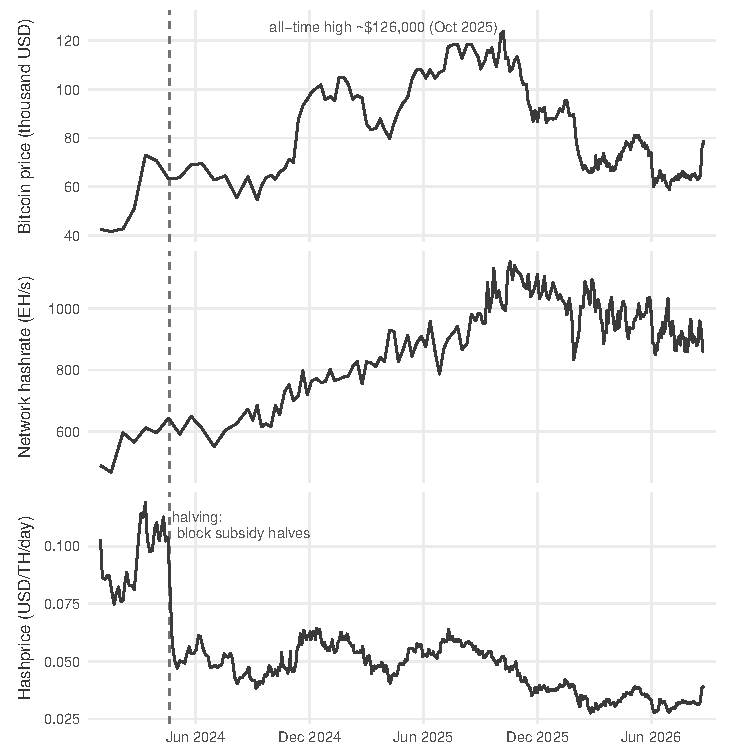
\includegraphics[width=\textwidth]{images/hashprice_cycle}
  \caption{
    The bitcoin price, the network hashrate, and hashprice, January 2024 to August 2026. Within a halving epoch, price and hashprice move together; across the April 2024 halving they decouple, because the halving cuts the newly issued bitcoin in half. The middle panel shows the network hashrate: every terahash that comes online dilutes the rest. Data: Braiins Insights \autocite{BraiinsInsightsHashprice}. % fig-src: analysis/figures/fig_ch4_hashprice_cycle.R (timeframes stitched to daily; Jan-Aug 2024 rests on the interpolated 5y frame)
  }
  \label{fig:hashprice-cycle}
\end{figure}

Does hashprice track the bitcoin price? Within a single halving epoch, yes, and increasingly tightly: the daily correlation between the two was 0.61 across 2025 and 0.90 in the 2026 bear leg. Across epochs, no: over the full window from January 2024 to mid-August 2026 the correlation is close to zero, because the halving sits in the middle of it. % src: Pearson r on stitched daily series, fig_ch4_hashprice_cycle.R console output 2026-08-24 (2025: 0.605; 2026 YTD: 0.901; full window: -0.08)
The bitcoin price rose by about two-thirds over that window; hashprice \emph{fell} by two-thirds. % src: BTC ~$42,600 (Jan 1, 2024) to ~$69,800 (Aug 12, 2026), +64%; hashprice $0.0921 to $0.0317, -66%; caches analysis/data/
Two structural forces produce that wedge. The halving cut the subsidy in half once, and relentless hashrate growth dilutes every survivor's share continuously. Hashprice rides the bitcoin cycle, but it rides it down an escalator.

The middle panel shows the machinery that connects the other two: a difficulty loop. A rising bitcoin price lifts hashprice at once. A high hashprice makes almost every machine on earth profitable, so more machines come online, and the network hashrate climbs: from roughly 490~EH/s in January 2024 to a peak above 1,100~EH/s in late 2025. % src: analysis/data/network_hashrate_daily.csv, the daily series the middle panel plots; analysis/checks/ch1_hashrate_peak.R console: 490.0 EH/s on 2024-01-01, daily max 1,151.5 EH/s on 2025-10-18, 7-day-mean peak 1,132.7 EH/s in the week to 2025-10-20 (fig_ch4_hashprice_cycle.R's console prints the same daily points rounded, 490 and 1151 EH/s)
Every new terahash raises the difficulty and dilutes each incumbent's share, which pushes hashprice back down. That is why the hashprice peaks of the 2024--2025 bull market kept coming in lower even as the bitcoin price kept setting records: each rally paid for the machines that diluted the next one. In 2026 the difficulty loop ran in reverse: hashprice fell below the breakeven of the fleet's weakest machines, machines switched off, and the hashrate in the middle panel rolls over, giving back a fifth to a quarter of its peak. % src: analysis/checks/ch1_hashrate_peak.R console: on 7-day means of analysis/data/network_hashrate_daily.csv, 1,132.7 EH/s (week to 2025-10-20) to 906.6 EH/s (week to 2026-08-24, the panel's last) is 20.0% given back, to 930.2 EH/s (week to 2026-08-21, ch1's anchor) 17.9%; on the daily points the panel plots, 25.4% (1,151.5 on 2025-10-18 to 859.1 on 2026-08-24; fig_ch4_hashprice_cycle.R's console: max 1151, 859 on 2026-08-24); ch1, ch4 and the glossary all date the peak to late 2025
Section~\ref{sec:sensitivity} shows what closes the difficulty loop at the level of a single machine.

The short run belongs to the bitcoin price, though, and it can move fast. In the week this chapter was drafted, a bitcoin rally of roughly a quarter lifted hashprice from \$0.031 to \$0.039 per terahash-day in eight days, tracking the price move almost one for one, because the difficulty happened to sit still the whole time. % src: stitched daily caches (analysis/data/): hashprice 0.0312 (Aug 16, 2026) to 0.0392 (Aug 24) = +25.6%; BTC 63,173 to 79,109 = +25.2%; difficulty 126.23T (Aug 6) to 125.81T (Aug 24), -0.3% (Braiins Insights difficulty series)
What that eight-tenths-of-a-cent move did to individual machines is the subject of the rest of this chapter.

\section{Efficiency: The Machine's Exchange Rate}

Hashprice prices computation. Electricity markets price energy. The bridge between them is the machine itself, and specifically the specification Chapter~1 called the most important one: efficiency, in joules per terahash (J/TH), the energy a machine spends to perform a unit of work. Efficiency is the exchange rate between the two currencies: it converts revenue per terahash into revenue per megawatt-hour, the number an energy trader actually wants.

The conversion deserves one careful derivation, because the book uses it constantly. A megawatt-hour is $3.6 \times 10^9$ joules. A machine with efficiency $e$ joules per terahash therefore performs $3.6 \times 10^9 / e$ terahashes per megawatt-hour consumed. Hashprice pays per terahash-day, which is $86{,}400$ terahashes, so one megawatt-hour earns:
\[
\text{revenue per MWh} = \text{hashprice} \times \frac{3.6 \times 10^9}{e \times 86{,}400} = \frac{41{,}667 \times \text{hashprice}}{e}
\]
with hashprice in \$/TH/day and $e$ in J/TH. % src: identity; constant 3.6e9/86,400 = 41,666.7; same form as the PAPO algorithm's revenue equation (papo-model-algo/PAPO_ALGORITHM.md)
The constant 41,667 is worth memorizing; it is the book's Rosetta Stone, and it will reappear in every Part III chapter.

Two machines carry the argument from here, chosen because together they bracket the working fleet. The \glossaryterm{antminer-s19j-pro}{Antminer S19j~Pro} is a 2021-vintage workhorse that still populates mining farms in large numbers: 104~TH/s at 3,068~W, which is 29.5~J/TH \autocite{bitmain2021s19jpro}. % src: Bitmain S19j Pro Specifications, 104T variant: 3068 W +/-5%, 29.5 J/TH (all variants); article created Jun 2021
The \glossaryterm{antminer-s21-xp}{Antminer S21~XP} is the 2024 flagship of the same manufacturer: 270~TH/s at 3,645~W, which is 13.5~J/TH \autocite{bitmain2024s21xp}. % src: Bitmain S21 XP Specifications: 3645 W on wall @25C +/-5% (4,000 W is the PSU requirement, not draw; some listings' 3,900 W is not Bitmain's rating); 13.5 J/TH; article created Jul 2024
The newer machine is not faster in any way that matters to this chapter; it is \emph{cheaper to feed}. At the 2025 average hashprice of about \$0.051 per terahash-day, the exchange-rate formula says the S19j~Pro turned each megawatt-hour into roughly \$72 of bitcoin, and the S21~XP turned the same megawatt-hour into \$157. % src: 41,666.7 x 0.0507 / 29.5 = 71.6; / 13.5 = 156.5; 2025 mean hashprice 0.0507 from analysis/data/hashprice_daily.csv
Under the same market conditions, the more efficient machine earns more than twice as much revenue per megawatt-hour.

\section{Breakeven: The Number That Runs the Business}

Set revenue per megawatt-hour equal to the price of a megawatt-hour and you get the number every mining operator knows by heart, the \glossaryterm{breakeven-price}{breakeven price}:
\[
P_{\text{breakeven}} = \frac{41{,}667 \times \text{hashprice}}{e}
\]
Read in this direction, it answers the operator's daily question: given today's hashprice, what electricity price can my machines afford? Solved for hashprice instead,
\[
\text{hashprice}_{\text{breakeven}} = \frac{e \times P}{41{,}667},
\]
it answers the investor's question: given my power contract, what hashprice keeps my machines alive? The two forms are one equation, and readers from either industry will need both.

To be precise, this breakeven is an \emph{operating} threshold. It compares revenue against electricity alone, and electricity is the dominant but not the only cost of running a mine; it ignores the capital cost of the machine, hosting, cooling, and staff. A machine below its operating breakeven loses money on every hour it runs and should stop immediately. A machine above it contributes margin, whether or not the site as a whole ever recovers its investment. Grid economics has the same distinction: this is the shutdown point, not the entry decision.

\section{Two Machines, One Hashprice}
\label{sec:sensitivity}

Now freeze everything except hashprice. Fix each machine at its stock operating point, so efficiency is a constant rather than a curve (the curve is Chapter~5's subject). Fix the electricity price at \$42.18 per megawatt-hour, the average 15-minute real-time settlement point price in LZ\_WEST across calendar 2025, the zone where this book's miners live; the market monitor's own accounting puts the zone's load-weighted average at \$41.59, the highest of any ERCOT zone that year \autocite{ercot2026rtm,potomac2026somercot}. % src: $42.18 = mean of all 35,040 15-min settlement prices, LZ_WEST 2025, from ERCOT MIS report 13061 (analysis/data/ercot_rtm15_spp_loadzones_2021on.csv.gz, built by analysis/data/fetch_ercot_rtm15_spp_history.py; console of analysis/figures/fig_ch6_strike.R). Supersedes the $42.22 of the older ingest cache, which dropped the nine spring-forward intervals; author confirmed $42.18 on 2026-09-04. The ERCOT-direct re-derivation pin is RESOLVED (2026-08-28). Cross-checks: 5-min series mean $41.79 (lz_west_rt_annual_means.csv); SOM load-weighted ex-adders $41.59 + ~$0.43 adders ~ $42.0. RT settlement is the book's reference price (author decision 2026-08-24)
A real ERCOT miner faces a different price every quarter-hour and that variance is where Part III finds its money; the flat average is deliberately artificial, a laboratory stand-in that isolates one variable. What remains is a clean experiment: sweep hashprice, watch two machines respond.

\begin{figure}[h]
  \centering
  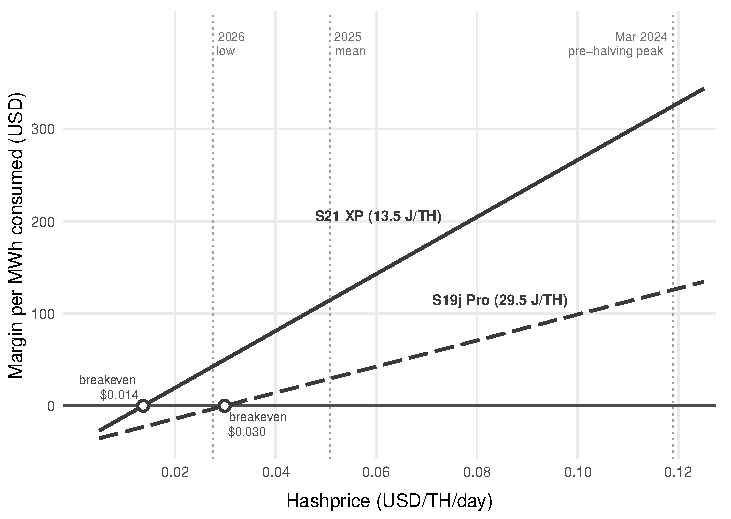
\includegraphics[width=\textwidth]{images/miner_sensitivity}
  \caption{
    Margin per megawatt-hour consumed as a function of hashprice, with efficiency fixed at stock and electricity fixed at the 2025 mean LZ\_WEST real-time settlement point price of \$42.18/MWh. Dotted verticals mark where hashprice actually traded: the March 2024 pre-halving peak, the 2025 mean, and the 2026 low. The S21~XP breaks even at \$0.014 per terahash-day, below anything the market has recorded; the S19j~Pro breaks even at \$0.030, a line the market crossed in 2026. % fig-src: analysis/figures/fig_ch4_sensitivity.R
  }
  \label{fig:miner-sensitivity}
\end{figure}

Figure~\ref{fig:miner-sensitivity} shows the result, and Table~\ref{tab:miner-sensitivity} gives the exact numbers at three hashprice levels the market actually visited: the 2026 low, the 2025 average, and the March 2024 pre-halving peak.

\begin{table}[h]
  \centering
  \small
  \begin{tabular}{lrr}
    \hline
    & \textbf{S19j Pro} & \textbf{S21 XP} \\
    \hline
    Hashrate & 104 TH/s & 270 TH/s \\
    Power draw (stock) & 3,068 W & 3,645 W \\
    Efficiency & 29.5 J/TH & 13.5 J/TH \\
    Electricity per day & 73.6 kWh & 87.5 kWh \\
    Electricity cost per day (at \$42.18/MWh) & \$3.11 & \$3.69 \\
    Breakeven hashprice & \$0.030 & \$0.014 \\
    \hline
    Profit per day at 2026 low (\$0.028) & $-$\$0.24 & +\$3.75 \\
    Profit per day at 2025 mean (\$0.051) & +\$2.18 & +\$10.02 \\
    Profit per day at Mar 2024 peak (\$0.119) & +\$9.26 & +\$28.42 \\
    \hline
  \end{tabular}
  \caption{Daily economics of the two machines at three hashprice levels. Stock specifications; electricity fixed at the 2025 mean LZ\_WEST real-time price. Profit here is revenue minus electricity only.} % src: computed in analysis/figures/fig_ch4_sensitivity.R (console output; landmarks read from the cache: 2024 max $0.11891 on 2024-03-13, 2025 mean $0.05082, 2026 min $0.02757 on 2026-02-24); hashprice landmarks from analysis/data/hashprice_daily.csv; RT mean from analysis/data/lz_west_rt_annual_means.csv
  \label{tab:miner-sensitivity}
\end{table}

Read the table bottom-up, from boom to bust. At the pre-halving peak, both machines printed money and the S19j~Pro's inefficiency did not threaten its margin; this is the regime in which nobody curtails and efficiency debates feel academic. At the 2025 average, the S19j~Pro still cleared about \$2 a day, a real but thinning margin. At the 2026 low, the two machines were no longer in the same business: the S21~XP still earned \$3.75 a day, while the S19j~Pro lost money every hour it ran.

The asymmetry has a name in any commodity industry: operating leverage. On the eve of the August 2026 rally, the S19j~Pro was spending 96 cents of every revenue dollar on electricity; the S21~XP was spending about 44. % src: at HP $0.0312 (Aug 16, 2026, pre-rally trough): S19j cost/rev = 3.11/3.24 = 0.96; S21 XP = 3.69/8.42 = 0.44; cost/day = W x 24h x $42.18/MWh: S19j 73.6 kWh -> $3.11, S21 87.5 kWh -> $3.69; rev/day = HP x TH: S19j 104 x 0.0312 = $3.24, S21 270 x 0.0312 = $8.42
A ten percent move in hashprice barely registers at the efficient machine and doubles or erases the inefficient one's entire margin. The week-long rally from \$0.031 to \$0.039 took the S19j~Pro from earning 14 cents a day to earning nearly a dollar, a sevenfold change, while the S21~XP improved by a comfortable but unremarkable half. % src: S19j: 104 x 0.0312 - 3.11 = +$0.14; 104 x 0.0392 - 3.11 = +$0.97; S21 XP: +$4.73 to +$6.89, +46%
Efficiency raises profits and reduces the machine's exposure to hashprice.

Here is the machine-level view of the difficulty loop in Figure~\ref{fig:hashprice-cycle}, and Chapter~2 already showed its fastest version in action. When hashprice falls below the breakeven of the fleet's marginal machines, those machines shut down; the network hashrate falls; the difficulty adjustment pays every surviving machine more; hashprice climbs back toward the new marginal breakeven. The network continuously reprices itself so that the worst machine still running earns roughly zero. % src: difficulty adjustment mechanism, Nakamoto2008; observed post-Fern: -11.16% adjustment then +14.73% recovery (ch2, BraiinsInsights)
That is why the S19j~Pro generation is not simply dead: every time enough of its cohort switches off, the survivors get a raise. The fleet lives on the breakeven line by construction, which means the marginal machine, wherever it is, mines for nearly nothing. Its only remaining edge is the price it pays for power.

\section{What This Means on a Grid}

Flip the breakeven formula one last time and it stops being an investor's metric and becomes an operating instruction. At any moment, a machine's breakeven price is the electricity price above which it is worth more switched off than on. At the 2025 average hashprice, the S19j~Pro's breakeven was about \$72 per megawatt-hour, a level LZ\_WEST real-time prices crossed routinely; the S21~XP's was about \$157, crossed far more rarely. % src: 41,666.7 x 0.0507 / 29.5 = 71.6; / 13.5 = 156.5; LZ_WEST exceedances quantified in ch6
In a market that reprices every few minutes (Chapter~3), that threshold is not a diagnosis. It is a tripwire: the moment the real-time price crosses it, the machine should stop, and the response can be automatic. The afternoon's day-ahead preview is still useful for flagging which hours look dangerous in advance, but the trigger itself is the real-time price. % src: reframed from "schedule" to reactive trigger per the ch6 RTM-strike decision (author, 2026-08-24)

The efficient machine survives expensive hours that kill the inefficient one, so efficiency buys \emph{endurance}. But the inefficient machine crosses its threshold more often, so it curtails more, and in programs that pay for flexibility it has more flexibility to sell. The S21~XP earns its money by running; the S19j~Pro increasingly earns its keep by knowing when to stop. Chapter~5 puts the two behaviors on one curve, because modern firmware lets a single machine slide between them; Chapter~6 turns the threshold into a strike price on the real-time market (a backstop that steps the machine out of price spikes) and prices the hours themselves. % src: ch6 strike analysis = RTM-reactive spike-avoidance backstop (author decision 2026-08-24; chapter 5's backstop implements it, analysis/ch5-backtest/papo_sim.py), NOT a day-ahead-scheduled strike

This chapter fixed efficiency and the power price to isolate hashprice. Every later chapter relaxes one of those clamps. Parts II and III look for the money in the variables this chapter held still.

\chapter{The Flexible Load: Curtailment and Power Optimization}
\chaptermark{The Flexible Load}
\label{ch:flexload}

Chapter~4 ended with a tripwire: above the breakeven price, a machine is worth more off than on. A tripwire is not an operating strategy. Prices arrive every five minutes, machines pay a real cost for every pause and resume, and the most expensive hours arrive with no warning at all. This chapter builds what actually pulls the trigger: first the power target (a machine's efficiency is not one number but a curve), then \glossaryterm{the-loop}{the loop}, the price-response layer that turns each new price into what the fleet draws, built on exactly three rules, and finally the report card, a benchmark against an oracle that sees the future.

\section{One Point Becomes a Curve}

Everything in Chapter~4 treated a miner as a fixed appliance: a fixed hashrate, power draw and efficiency. That is how stock firmware ships. Modern autotuning firmware removes the assumption: it can hold the machine at any \glossaryterm{power-target}{power target} across a wide range, retuning each hashing chip as it goes, and the single operating point opens into an \glossaryterm{efficiency-curve}{efficiency curve}. Figure~\ref{fig:efficiency-curves} shows two of them, for the two machines of Chapter~4, and their provenance matters: these are not laboratory curves but \emph{fleet averages}, aggregated from the operating data of miners running Braiins~OS in the second quarter of 2026, which this book calls the fleet dataset. % src: Braiins OS fleet telemetry aggregates, quarter 2026-Q2, the author's employer's data; cache analysis/data/miner_efficiency_telemetry_2026q2.csv
Remember which direction is good: efficiency counts the joules spent per unit of hashing work, so a \emph{lower} number means less energy for the same output. Run the S19j~Pro below its stock 3,068~W and its efficiency improves: the fleet average bottoms out at 23.8~J/TH near 1,200~W, against a nameplate of 29.5, because chips run more efficiently at lower voltage and frequency. % src: telemetry cache analysis/data/miner_efficiency_telemetry_2026q2.csv (telemetry refreshed 2026-08-27): best 23.83 J/TH at 1,200 W; nameplate per bitmain2021s19jpro
Push it above stock and it buys extra hashrate at ever-worse efficiency, up to the \glossaryterm{power-ceiling}{power ceiling}, the highest power target the loop will set, here 3,420~W for the S19j~Pro and 3,990~W for the S21~XP. Efficiency, the exchange rate of Chapter~4, turns out to have a throttle attached. % src: ceilings analysis/ch5-backtest/papo_sim.py PARAMETRIC_MINERS p_max 3420 and 3990, kept by telemetry_miner.py build() (its console: floor / default / ceiling 1200 / 3068 / 3420 and 2774 / 3645 / 3990 W), as chapter 9 (analysis/checks/ch9_tuning.R header), below the telemetry extent, 4,400 and 4,600 W; no PSU rating is printed: bitmain2021s19jpro gives none, and bitmain2024s21xp gives an adapted AC output power requirement of 4,000 W (read 2026-09-26, article updated 2026-09-23); Bitmain's PSU pages, read 2026-09-26 through support.bitmain.com/api/v2/help_center/en-us/articles/<id>.json, map the S19j Pro to the APW12 family (15909673875993) and the S21 XP to APW171215a/c or PW380a/b/c (47856379027737), and rate APW12 at up to 240 A at 15 V, 3,600 W (900001205726), and APW171215a at 267 A, at most about 4,005 W at 15 V (32499285460505); so the S19j Pro ceiling sits 5% under its PSU but the S21 XP ceiling only about 0.4% under, and the earlier clause about a margin below the power supply rating is withdrawn

\begin{figure}[h]
  \centering
  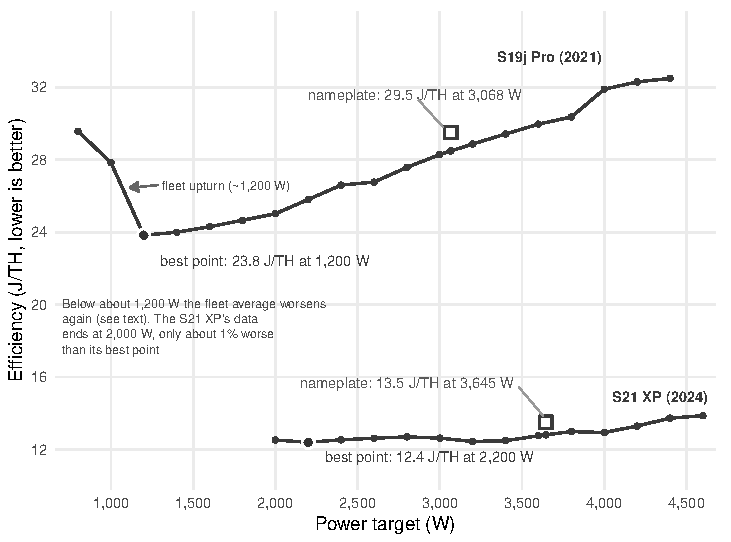
\includegraphics[width=\textwidth]{images/efficiency_curves}
  \caption{
    Measured efficiency curves for the Antminer S19j~Pro and S21~XP: fleet averages of operating data from miners running Braiins~OS, second quarter of 2026. Lower is better. Squares mark the manufacturer nameplate at stock power; filled dots mark each curve's best-efficiency point. The arrow marks where the S19j~Pro's fleet average turns back up, near 1,200~W (see text). The S21~XP's lowest reading, at 2,000~W, is just 1~percent worse than its best point. The loop's power ceilings, 3,420 and 3,990~W, stop short of the curves' right-hand ends; its modulation floors are 1,200~W and, on the S21~XP, Braiins~OS's default minimum, 2,774~W. % fig-src: analysis/figures/fig_ch5_efficiency_curves.R (telemetry cache analysis/data/miner_efficiency_telemetry_2026q2.csv; Braiins data); the modelled V-floor, 1,850 to 1,900 W, is internal Braiins modeling (one engineer's fitted curves, a personal communication) as analysis/checks/ch5_vfloor.py part 2 transcribes it; 1% is analysis/checks/ch5_vfloor.py part 1 (S21 XP 2,000 W +1.03% on the 2,200 W best point); ceilings 3,420 and 3,990 W as the power-ceiling sentence above (analysis/ch5-backtest/papo_sim.py p_max), curves end at 4,400 and 4,600 W; floors 1,200 W (the S19j Pro's best point) and 2,774 W (the S21 XP's Braiins OS default minimum, braiinsacademytechres) as analysis/ch5-backtest/telemetry_miner.py modulation_floor takes them (analysis/checks/ch5_vfloor.py part 3)
  }
  \label{fig:efficiency-curves}
\end{figure}

Two caveats belong to these curves. First, the nameplate is not the field. A machine's rated efficiency is measured on fresh hardware under factory settings; on a real site, every unit differs. Chips vary in quality straight from the fab, the spread miners call the silicon lottery, and machines age: fans wear, thermal interfaces dry out, dust accumulates. The curves here average the machines running Braiins~OS in this dataset; an individual machine sits somewhere around them, not on them. At stock power the autotuned fleet average actually \emph{beats} the nameplate, 28.5 against 29.5~J/TH for the S19j~Pro and 12.8 against 13.5 for the S21~XP, because per-chip tuning recovers headroom that factory firmware, with one setting for every unit, has to leave on the table. % src: telemetry at 3,068 W = 28.48 J/TH (S19j Pro); at 3,645 W = 12.81 vs 13.5 nameplate (S21 XP)

Second, the curve has a bottom, and it is not at zero watts. Below roughly 1,200~W the S19j~Pro's fleet average turns back up. I read such a bottom as the power supply's doing, the \glossaryterm{v-floor}{V-floor}. Modeling work at Braiins supports that mechanism.\footnote{Based on internal modeling work at Braiins.} On the S19j~Pro, at clock speeds of about 300~MHz and below, the hashboards would need less voltage than the supply's minimum output, 12~volts on the APW12 and APW17 supplies Bitmain lists for these machines \autocite{bitmain2025psu}. Past that point only the frequency drops. % src: internal Braiins modeling: Pavel Mikuš, Performance Curves of the Antminer S19j Pro, S21 XP and S21 Pro, personal communication, October 15-16, 2025; Braiins is the author's employer (one engineer's personal communication, internal chat of 15 Oct 2025, on his modelled S19j Pro curve: the sharp break a bit below 2,000 W is where the miner hits the PSU's minimum voltage; at about 300 MHz or below the chips do not need that much voltage, but the PSU cannot go lower, so below the floor only the frequency drops and the extra voltage turns into heat; the 300 MHz is given for the S19j Pro only, no break frequency for the S21 XP or S21 Pro), confirming the mechanism of the author's earlier reading, not the fleet's 1,200 W upturn (the model's break is 650-700 W higher, the reconciliation below), printed as such until 2026-09-26 (STATUS, open item 2); bitmain2025psu (article 15909673875993): S19j Pro on the APW12 (12V-15V) series, S21 and S21 Pro on APW171215a/c or PW380a/b/c under the heading APW17 (12V-15V), PW380; article 47856379027737 gives the S21 XP the same APW171215a/c or PW380a/b/c; the APW12 and APW171215a spec sheets (900001205726, 32499285460505) give OUT1 DC voltage 12V-15V; all four read 2026-09-26 through support.bitmain.com/api/v2/help_center/en-us/articles/<id>.json; PW380 has no published spec, so the 12 V is printed for the APW12 and APW17 only; the upturn itself is in the telemetry cache: S19j Pro 800 W = 29.6 J/TH vs 1,200 W = 23.8 (analysis/checks/ch5_vfloor.py part 1)
The chips then run on more voltage than they need, which forfeits the quadratic voltage saving that made underclocking efficient in the first place: the energy the surplus voltage costs goes into heat, not hashing. Meanwhile the chips' leakage at the pinned voltage, the fans and the control board keep drawing a fixed share, now spread over ever less hashing. Whatever sets a curve's bottom, running below it is strictly worse than running at it: less work \emph{and} worse efficiency. % src: internal Braiins modeling (below the floor the chips run on more voltage than they need, only the frequency drops, and the extra voltage turns into heat); the quadratic voltage saving and the fixed draw (leakage at the pinned voltage, fans, control board) are the author's physics, which the repository does not show beyond one line of arithmetic: the modelled S19j Pro's constant gain below its floor, +2.525 TH/s per 50 W through 73.44 TH/s at 1,850 W, puts about 396 W on a line that does not scale with hashrate, more than fans and a control board draw (analysis/checks/ch5_vfloor.py part 2, an intercept of the quoted line, not a modelled reading); a curve's bottom is its best-efficiency point, below which it has less hashrate and worse J/TH (part 1: S19j Pro 800 and 1,000 W, S21 XP 2,000 W)

The V-floor is a voltage limit, not a fixed wattage; where it falls depends on the type of machine. % src: internal Braiins modeling as transcribed in analysis/checks/ch5_vfloor.py MODELLED (part 2 console): S19j Pro floor about 1,850-1,900 W, 74-76 TH/s (per 50 W step from 1,800 W +2.525, +2.380, +1.293 TH/s; best 25.06 J/TH at 1,900 W; hashrate stops growing at about 5,350 W, 149 TH/s, the PSU's maximum voltage); S21 XP about 1,900-1,950 W, 178 TH/s (a flat +6.685 per 50 W to 1,900 W, then +6.626 and +4.902); S21 Pro about 1,650 W, 122 TH/s (a flat +5.816 to 1,650 W, then +5.14); 1,925 W is the midpoint of the S21 XP's 1,900-1,950 W; the same supply per bitmain2025psu (S21 XP and S21 Pro both APW171215a/c or PW380a/b/c); the caveats are internal Braiins modeling's: a fitted model, a year of telemetry, 42 C average hashboard temperature (which the engineer calls the bosminer default for the model; not the Academy's Default Temperatures, braiinsacademytechres, whose 60 C for the S19J Pro and 65 C for the S21 XP and S21 Pro are target temperatures, a different quantity), errors from Braiins' own power model, not comparable with manufacturer marketing specs

Figure~\ref{fig:efficiency-curves}'s fleet averages do not pinpoint that limit for an individual machine. % src: (2026-10-13, author decision: the prose and the Figure 5.1 caption print only the fleet's 1,200 W, not the modeled single-machine floor of about 1,850-1,900 W, which stays in these notes)  analysis/checks/ch5_vfloor.py part 2 console: S19j Pro fleet at 1,850 and 1,900 W (interpolated) 74.75 and 76.48 TH/s against the model's 73.44 and 75.82 (+1.8%, +0.9%); below the floor the model gains +2.525 TH/s per 50 W, the fleet +1.888 over 1,200-1,800 W (75% of it), and fleet J/TH falls from 24.66 at 1,800 W to 23.83 at 1,200 W (-3.3%); S21 XP fleet best point 2,200 W, 177.47 TH/s (-0.3% on the model's 178); 2,200 W against the model's 1,900-1,950 W is +12.8% to +15.8% (+14.3% on the 1,925 W midpoint); 2,000 W is +1.03% J/TH on 2,200 W and 10.3% below the modelled floor's hashrate; part 1: S21 XP range 12.40-13.87 J/TH over 2,000-4,600 W; the kit's S21 XP floor is not this best point but Braiins OS's default minimum, 2,774 W (analysis/ch5-backtest/telemetry_miner.py modulation_floor, the next paragraph; the retired parametric floor, 2,760 W, runs only under PAPO_PARAMETRIC=1)
% Historical provenance (detail removed from prose on 2026-10-02): the three candidates are the author's reading (2026-09-26), not a finding: the repository cannot test them, because the committed telemetry has no temperature, sample-count or power-source field (analysis/data/miner_efficiency_telemetry_2026q2.csv carries model, power_w, avg_jth and hashrate_ths, and hashrate_ths is power_w / avg_jth); errors from Braiins' power model are internal Braiins modeling's own caveat; the second candidate is braiinsacademytechres, read 2026-09-26: Supported Devices gives the S19J Pro's original PSUs as APW121215a/b/c, and Supported PSU Models gives Power readings: No for APW121215a/b/c (and d/e/f/g), Yes for APW171215a/c, the S21 XP's; Figure 5.1's x axis is the power target, and the CSV's hashrate_ths is power_w / avg_jth
The backtests in this chapter and Chapter~9 use the measured fleet curves. In them the lowest power target is 1,200~W for the S19j~Pro, its best-efficiency point, and 2,774~W for the air-cooled S21~XP, the Braiins~OS default minimum. The latter is a firmware setting, not a claim about the machine's physical limit \autocite{braiinsacademytechres}. % src: braiinsacademytechres, Default Power Limits, read 2026-09-26: Min Power 944 W (S19J Pro, every variant, 2,478 to 3,068 W) and 2,774 W (S21 XP, 3,645 W, 270 TH/s), with 2,316 W for the S21 Pro and Max Power 6,435 W for all three (transcribed in analysis/checks/ch5_vfloor.py ACADEMY); the page warns that pushing a miner to its minimum limit reduces efficiency; analysis/checks/ch5_vfloor.py part 3: 944 W is below the modelled 1,850-1,900 W and 2,774 W above the modelled 1,900-1,950 W; fleet readings below the defaults: S19j Pro 800 W, S21 XP 2,000, 2,200, 2,400 and 2,600 W; the S21 XP's best point, 2,200 W, is part 1 and Figure 5.1; the kit and chapter 9 floor the S21 XP at the default, 2,774 W, the author's decision of 2026-09-26 (analysis/ch5-backtest/telemetry_miner.py modulation_floor and BOS_DEFAULT_MIN_W; analysis/checks/ch9_tuning.R ch9_floor and CH9_BOS_MIN_W; ch5_vfloor.py part 3 console: modulation floor S21 XP 2,774 W, the default minimum, and S19j Pro 1,200 W, the best-efficiency point, its default 944 W being lower), until then at its 2,200 W best point
% Historical provenance (detail removed from prose on 2026-10-02): bitmain2024s21xp (270 TH/s at 3,645 W, rated at inlet air temperature, noise with the fan at max RPM); braiinsacademytechres, re-read 2026-09-27, Default Power Limits: Antminer S21 XP 3,645 W (min 2,774 W, 270 TH/s), S21 XP Imm. 4,050 W (min 2,877 W, 300 TH/s), S21 XP Hyd. 5,280 and 5,676 W (min 3,863 W, 440 and 473 TH/s); analysis/data/miner_efficiency_telemetry_2026q2.csv has model, power_w, avg_jth and hashrate_ths and no cooling field (its S21 XP is the 270 TH machine, analysis/data/README.md)

That throttle, the power target, converts the price signal into something much better than on/off. For any electricity price there is one point on the curve that maximizes profit, which is revenue minus energy cost, and on a linear efficiency model it has a closed-form solution the loop can recompute cheaply. The backtests at the end of this chapter pick the most profitable point on the measured curve itself. Figure~\ref{fig:optimal-power} plots it for the S19j~Pro: cheap hours push the optimum to the power ceiling, expensive hours walk it down the curve, and the walk stops at the \glossaryterm{modulation-floor}{modulation floor}, the lowest power target the loop will set. Those are the two lowest targets given above. Below the S19j~Pro's, slowing down further surrenders more hashrate than the electricity it saves, so no price justifies going there gradually, even though Braiins~OS's default minimum lies lower. The S21~XP's is Braiins~OS's default minimum itself, which sits above that machine's best point. Past the floor there is only one move left, the full pause, and the loop deliberately hands that decision to a different rule with different physics. This gradual repricing of a running machine is \glossaryterm{modulation}{modulation}; the pause is not its job.

\begin{figure}[h]
  \centering
  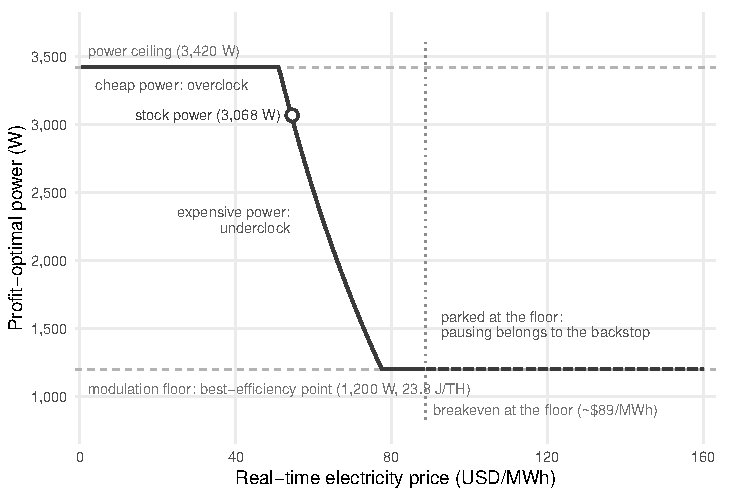
\includegraphics[width=\textwidth]{images/optimal_power}
  \caption{
    What the loop computes: the profit-optimal power level as a function of the real-time price, for the S19j~Pro, using the closed-form solution on its linear-efficiency model fitted to the measured 2026-Q2 curve. Cheap power pushes the machine to its power ceiling; expensive power walks it smoothly down to the modulation floor at the best-efficiency point. Past the floor's breakeven, the target parks (dashed): pausing belongs to the backstop, not to modulation. Hashprice held at its 2025 mean. % fig-src: analysis/figures/fig_ch5_optimal_power.R (closed form per papo_sim.py Miner; anchored to the telemetry's best point and stock value, so figs 5.1/5.2 share one source; optimizing the raw fleet-average spline instead yields artificial steps from averaging lumps -- author caught this 2026-08-28)
  }
  \label{fig:optimal-power}
\end{figure}

\section{Three Facts That Shape the Control Problem}

Designing the reflex around that curve means respecting three facts about the environment it lives in.

First, the price feed is fast, noisy, and mean-reverting. ERCOT publishes a new real-time price every five minutes (Chapter~3); this book borrows the trading floor's word for each published number and calls it a \glossaryterm{print}{print} (ERCOT's own documents call it a Locational Marginal Price, or LMP, and keep settlement point price for the 15-minute price built from those). Five-minute price \emph{changes} are negatively autocorrelated: at LZ\_WEST, from 2024 to mid-2026, the correlation between one change and the next is about $-0.29$. The spikes carry that number. Each of the five largest leaps in the record, all of more than \$4,000, fell straight back at the very next print, so a run-up of that kind predicts a pull-back, not a continuation. Ordinary moves of a few dollars carry almost no signal either way, and in the first half of 2026, when no single print rose by more than \$700, the figure was about zero. % src: analysis/checks/ch5_price_autocorrelation.py, LZ_WEST five-minute prints 2024-01-01..2026-06-22 Central (260,337 change pairs): lag-1 autocorrelation of changes -0.294 (rank/Spearman +0.079); five largest up-moves +4,123 to +4,745, each followed by -4,393 to -4,883; without the 10 largest moves -0.167, without every print above $500 -0.123; by half-year -0.307, -0.266, -0.263, -0.434, +0.020 (2026-H1), with the largest one-print rise +4,431, +4,537, +4,368, +4,745 and +694 (2026-H1 still had 32 prints above $1,000, in runs, not leaps). On the 15-minute settlement series the eight zones run -0.052 to +0.013 (LZ_SOUTH positive), so the figure is a five-minute, spike-driven statistic; the loop decides on the five-minute prints
Whatever the price just did is a bad guide to what it does next; the level, not the trend, carries the information.

Second, wear is real. A fleet that re-applied its optimal target on every print would move about thirty times a day on the S19j~Pro, and about three times on the S21~XP (whose target sits at its power ceiling almost all the time), mostly chasing wiggles worth pennies, and would pause and resume hardware on noise. % src: analysis/ch5-backtest/output/trend_study/sweep_results.csv, persist hold5 (retarget on every print), TEST-2025-26 changes_day 32.0 (S19j Pro) and 2.8 (S21 XP); TUNE-2024 26.9 and 2.9
Moving the target is not always free, and pausing never is. A move to a power target the machine has no saved tuning profile for sends the autotuner walking every chip to new voltage and frequency settings, so the machine hashes below its optimum for the settling period of that tuning run. A target it already holds a profile for can be applied again without a new run, but only that exact target \autocite{braiinsacademyautotuning,braiinsacademydps}. % src: braiinsacademyautotuning, read 2026-09-25 (the hashrate fluctuates noticeably while a machine tunes; once tuning finishes the profile is saved and can be applied again later without waiting for a re-tune); braiinsacademydps, Grid Alignment, re-read 2026-09-26 (with a 3,500 W target and 300 W steps the sequence is 3,200, 2,900, 2,600 and 2,300 W; a start at 66% gives 2,310 W, which is snapped to 2,300 W, since keeping 2,310 would create another sequence of targets that would need to be tuned, slowing the operation and lowering the hashrate); that the reuse holds for the exact target only is also the author's account (2026-09-26); the settling period is the author's round-3 request (2026-08-27), and no duration is printed because Braiins pages disagree on one: about 10 minutes on the Autotuning and About pages, several hours depending on model and control board on the FAQ page (academy.braiins.com/braiins-os/faqs/dps-autotuning), which also says a settled tune can restart after a large change in chip temperature
That cost falls once per target, and the loop uses only a handful.
In this chapter's backtests, once a run has left stock power, it applies only the corner points of its fleet's curve, the targets that can maximize profit as electricity prices change, including the power ceiling: four targets on the S21~XP (2,774, 3,200, 3,400 and 3,990~W) and eight on the S19j~Pro. % src: analysis/ch5-backtest/optimizer_bruteforce_check.py console, re-run 2026-09-26 on the S21 XP's 2,774 W floor: upper concave hull S21XP 2774, 3200, 3400, 3990 W and S19jPro 1200, 1400, 1600, 1800, 2000, 2600, 3400, 3420 W, all on the engine's scan grid (the floor, then every 10 W); the corner points are the hull points, a point no straight line between two others passes above, and the two ceilings, 3,990 and 3,420 W, and the S21 XP's floor, 2,774 W, lie between measured points (3,800 / 4,000, 3,400 / 3,600 and 2,600 / 2,800 W), so they are corners of the curve the engine runs, not measured points; with the floor at the 2,200 W best point the S21 XP's four were 2,200, 3,200, 3,400 and 3,990 W; the claim covers the chapter 5 kit only: its curves (telemetry_miner.py) interpolate hashrate linearly between the measured points of analysis/data/miner_efficiency_telemetry_2026q2.csv and optimal_power() scans them at 10 W from the floor, so profit is piecewise linear in power and peaks on a hull point whatever the price; its "targets the loop applies" block runs every configuration of mixed_basis_study.py at LZ_WEST in TUNE-2024 and TEST-2025-26, 20 runs per fleet, and finds 4 of 4 and 8 of 8 hull points applied, no other target, and stock power only in the 26 intervals per fleet before each run's first move; papo_sim.py simulate() sets the target only to stock power or to an optimal_power() result (or to fixed_power, which only baselines_study.py passes, and only as the power ceiling, a hull point), so every other driver in the kit is bound the same way; chapter 9's engine is not bound to these points: analysis/checks/ch9_tuning.R ch9_curve interpolates J/TH on a 100 W grid and sets hashrate to power / J, which bends between measured points, and ch9_tune and ch9_tune_site may pick any grid point
Each needs one tuning run, unless a large swing in chip temperature restarts it, and every later visit reuses the saved profile \autocite{braiinsacademyautotuning}.
A pause costs more: the machine earns nothing while paused, and although a resume ramps its power back up in about 30 seconds \autocite{braiinsacademyramping}, every full thermal cycle, the boards heating and cooling through tens of degrees, spends a little of the hardware's life. % src: braiinsacademyramping, read 2026-09-27: Quick Ramping, the sequence used when the miner is resuming from a paused state, approximately 30 seconds; ramping also runs in reverse when a miner is paused, for the same time; was "hashing returns within seconds of a resume", per the author 2026-08-28 (a paused machine stays powered); the wear cost is the thermal cycle, not the ramp, which is the author's account
That pause is the firmware's: the machine stops hashing on a pause command but stays powered, its fans still under the firmware's control \autocite{braiinsacademyminerstates,braiinsacademyadvanced}. Opening a breaker, the way Chapter~\ref{ch:ancillary}'s relay-tripped load comes off, is a different act, after which every machine boots, ramps and warms up again. % src: braiinsacademyminerstates, read 2026-09-27 (Mining paused by user: the miner has received a pause command, for example from software used for curtailment); braiinsacademyadvanced, read 2026-09-27 (Control fans PWM after PAUSE: the fans are controlled after the miner enters the PAUSE state, 20% PWM by default, in the GUI's Cooling section since 25.05); that it stays powered is the author's account (2026-08-28) and follows from both; braiinsacademyramping (Normal Ramping, for booting up or restarting, about 30 s, then pre-heating the hashboards, with a timeout of about 10 minutes); chapter-7.tex sec:clr (the under-frequency relay trips the breaker within half a second)
The loop must move only when moving pays.

Third, the stakes are wildly asymmetric. One full-power hour at \$1,600 per megawatt-hour costs an S19j~Pro about 22 times the revenue it earns at 2025's mean hashprice and about 34 times at the lower mean of 2026 to date; for the S21~XP the same hour costs about 10 and 15 times what it earns on those two bases. % src: analysis/checks/ch5_stakes.py section 1: $1,600 / (41,666.7 x mean hashprice / J/TH), on the gap-filled daily hashprice as ch9_hashprice.R builds it; 2025 mean $0.0508/TH/day (365 days), 2026-01-01..08-29 mean $0.0338 (241 days, the window chapter 10 calls 2026 to date); nameplate 29.5 J/TH 22.31x and 33.54x, 13.5 J/TH 10.21x and 15.35x; at the engine's power ceiling on the telemetry curve (3,420 W at 29.47 J/TH, 3,990 W at 12.94 J/TH) 22.29x/33.51x and 9.78x/14.71x, so stock and full power round alike
Such hours are rare but real: LZ\_WEST's settlement point price averaged \$1,600 or more over a full clock hour five times in 2024 and twice in 2025, and the worst hour of 2026 to date, at \$1,330, still cost the S19j~Pro about 28 times what it earned at that period's mean hashprice. % src: analysis/checks/ch5_stakes.py section 2, MIS 13061 LZ_WEST clock hours (Central) whose four intervals average >= $1,600: 5 hours on 3 days (2024), 2 on 2 days (2025, highest $1,905.61 on 2025-01-15 07:00), none 2026-01-01..08-29 (highest $1,329.65 on 2026-01-28 07:00: 27.9x at the period mean hashprice on 29.5 J/TH, the basis of the sentence before; 23.7x at that day's $0.0398); five-minute prints >= $1,600: 54 on 12 days (2024), 22 on 5 days (2025), 0 to 2026-06-22; median five-minute print at or above $1,000: $1,770 (2024), $2,015 (2025)
Missing a spike is catastrophic; a false alarm costs a few minutes of hashing. Any design that treats those two errors symmetrically is wrong.

So the loop has three jobs with three different tempos: follow the price level cheaply and continuously, ignore the noise so hardware survives, and pause decisively when a spike is real. Each job gets its own rule.

\section{One Loop, Three Rules}
\label{sec:threerules}

The loop separates two functions: \emph{modulation reprices the fleet; the} \glossaryterm{backstop}{backstop} \emph{owns pause and resume}. The two mechanisms read the same price feed and never share a decision, which is what keeps noise out of the pause/resume path.

\subsection{Rule 1: Follow the Level}

Every five minutes, the loop recomputes the profit-optimal power target of Figure~\ref{fig:optimal-power} from the newest print, unmodified. Using the last print as the decision price is called \glossaryterm{persistence}{persistence}, and it is a measured choice; the case against forecasting comes below. The target is clamped between the modulation floor and the power ceiling. A print is already in force before anyone outside ERCOT can read it. ERCOT stamps each price with the moment it takes effect and publishes it straight after the SCED run that sets it \autocite{ercot2026protocols}: the posting lands a median 22 seconds after the five-minute boundary. % src: analysis/checks/ch5_posting_latency.py console, on ERCOT's public MIS listing of NP6-788 (reportTypeId 12300) as snapshotted by analysis/data/fetch_ercot_np6788_posting.py: 1,569 on-cycle SCED runs 2026-09-20..25 Central (5.4 days, 0 missing windows), posted median 22 s / p95 28 s after the five-minute boundary, SCED stamp median 19 s after it; ercot2026protocols sec. 6.3.2(2): LMPs posted immediately subsequent to deployment of Base Points and Ancillary Service awards from SCED, with the time stamp the prices are effective; the print stamped b prices [b, b+5) at zero lag (analysis/ch5-backtest/ingest/verify_alignment.py); when a posted print becomes readable is not measured (a listing probe timed a CDN cache, not ERCOT, and was withdrawn 2026-09-25)
Reading it takes longer. Polled through ERCOT's public API every 20 seconds for ten days in autumn 2026, a print became readable a median 2.9~minutes after its boundary, and 3.5~minutes in the evening hours, so more than half of its own interval is gone before the loop can act on it. % src: analysis/checks/ch5_api_readability.py console, on analysis/data/ercot_api_readability_polls.csv.gz (37,780 polls 2026-09-25 02:11 to 2026-10-05 02:11 Central, written by analysis/data/ercot_api_readability/poll.py, one poll every 20 s, arrival timed at the midpoint between successful polls): NP6-788 full window n=2,448 on-cycle prints, median 172.0 s after the five-minute boundary (2.87 min), p95 296.0 s; 18:00-22:00 Central median 212.0 s (3.53 min), other hours 169.0 s; the clean window without the 2026-09-30..10-02 connection outage gives a median of 171.0 s
The backtests assume a full interval of delay before the loop sees each print, which covered 95~percent of the prints polled; in them it is always steering on the most recent past, never the present. % src: analysis/checks/ch5_api_readability.py console, "readable within one five-minute interval of its boundary: 2332 of 2448 = 95.3%"; the other 4.7% (116) arrived later, max 887 s

\subsection{Rule 2: Ignore the Noise}

Computing a target every five minutes does not mean applying it every five minutes. By default the applied target holds for 30 minutes. A plain hold has a flaw, though: when the price gaps to a new level, the fleet can run up to 25 minutes on a stale target. The fix is the \glossaryterm{price-deadband}{price deadband}, one extra condition on the hold: re-apply immediately whenever the newly computed ideal target diverges from the applied one by more than 10~percent of the machine's stock power. Figure~\ref{fig:deadband} shows the two behaviors on one trace. In the calm stretches the price deadband never fires and the wear profile is identical to the plain hold; each time the price gaps, up and then back down, it fires once, and the fleet reprices within five minutes instead of thirty. % src: analysis/figures/fig_ch5_deadband.R console: deadband fires 2 times, at 80 and 135 min, on the gaps at 75 and 130 min; largest ideal-vs-applied gap in the calm stretches 116 W against a 307 W deadband

\begin{figure}[htbp]
  \centering
  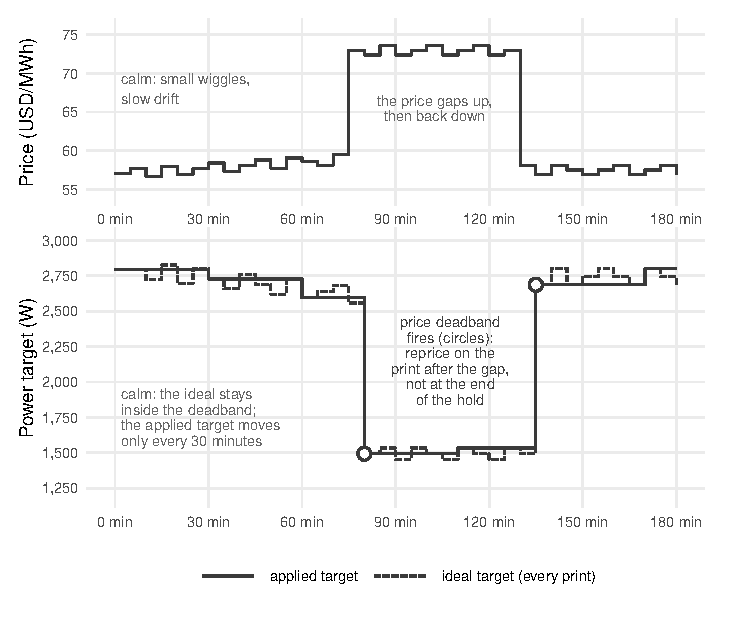
\includegraphics[width=\textwidth]{images/deadband}
  \caption{
    The 30-minute hold and the price deadband that breaks it, on an illustrative price trace, for the S19j~Pro on the same model and optimizer as Figure~\ref{fig:optimal-power}. Through the calm stretches the ideal target (dashed) wiggles inside the price deadband, so the applied target (solid) moves only on the routine 30-minute cadence. When the price gaps up, and again when it gaps back down, the ideal diverges by more than 10~percent of stock power, the price deadband fires (circles), and the fleet reprices on the next print instead of waiting out the hold. Each price print is seen one interval late. % fig-src: analysis/figures/fig_ch5_deadband.R (illustrative trace; measured constants: 30-min hold, deadband 10% of 3,068 W = 307 W, each print seen one interval late; linear-efficiency model anchored at the telemetry's 1,200 W best point and at stock, as fig 5.2; console: fires 2 times, at 80 and 135 min)
  }
  \label{fig:deadband}
\end{figure}

On the older fleet the price deadband is worth real money, and it is not free. In the out-of-sample backtest at the end of this chapter, it adds 2.6~percent to what the plain hold earns over running at stock power on the S19j~Pro fleet, for about 26 target moves a day against the hold's 13. The S21~XP's flat curve leaves it less to do: 0.5~percent more, at under three moves a day. % src: analysis/ch5-backtest/output/trend_study/mixed_basis.csv, TEST-2025-26, LZ_WEST, 5-minute feed, plain hold (decide-5 S14) vs deadband 10% (decide-5 +deadband10): vs_basis_s14 +2.5559 (S19j Pro) and +0.4723 (S21 XP), the deadband's gain as a share of the plain hold's gain over stock power; pct_of_s1 93.85 -> 96.25 and 97.61 -> 98.07; changes_day 13.4 -> 26.3 and 1.6 -> 2.4; on the S21 XP's 2,774 W floor (+0.7535, 2.6 moves a day, on its 2,200 W best point until 2026-09-26)
The backtest charges nothing for a move, so both gains are counted before whatever the extra moves cost on a given fleet's firmware. % src: analysis/ch5-backtest/papo_sim.py simulate(): once the hold or the price deadband allows it, applied = ideal within the same interval and profit is booked at full curve efficiency, with no per-move charge (changes counts the moves and nothing else)
The price deadband is also a dial rather than a knife-edge on the S19j~Pro: widening it to 25~percent keeps about four-fifths of the benefit while cutting the extra moves roughly in half, which makes it the one knob worth handing an operator with a wear budget. The S21~XP has little to trade: at 25~percent its extra moves, under one a day, all but vanish, and it keeps under a quarter of the benefit. % src: analysis/ch5-backtest/mixed_basis_study.py console "dial" lines, TEST-2025-26: deadband25 keeps 82% (S19j Pro) and 23% (S21 XP) of deadband10's gain over the plain hold, at +6.0 and +0.0 moves/day above the hold against +12.9 and +0.8 for deadband10 (changes_day 1.6 for both the S21 XP's plain hold and deadband25); in the 2024 tuning year it keeps 93% and 19%; on the S21 XP's 2,200 W best point, its floor until 2026-09-26, the S21 XP kept 64% (2024: 65%) at +0.5 against +1.0

\subsection{Rule 3: Survive the Spikes}

Pausing hardware is expensive, and five-minute prices mean-revert, so the backstop does not pause just because a print crosses breakeven. It reacts to \emph{accumulated damage}. While the price sits above the machine's breakeven at its most efficient power target within the loop's operating range (on the S21~XP 3,200~W, above its floor), the excess integrates: each print adds its excess over breakeven multiplied by the time it covers, which is what one megawatt at that target loses at that price. The moment the total reaches \$10 per megawatt, the fleet pauses. % src: analysis/ch5-backtest/papo_sim.py K_TRIP = 10.0 ($ per MW), applied in simulate(): while running, area += (p_prev - be_val) * dt_h when p_prev >= be_val and area = 0 when p_prev < be_val, pause once area >= K_TRIP (subject to MIN_UP_S and MAX_CYCLES_DAY); $/MWh x h = $ per MW of load; be_val = breakeven_best(hashprice) of the engine miner, in the default telemetry mode analysis/ch5-backtest/telemetry_miner.py TelemetryMiner.breakeven_best (best breakeven over the engine's power range, floor to ceiling: at 1,200 W on the S19j Pro, its modulation floor, and at 3,200 W on the S21 XP, above its 2,774 W floor; papo_sim.py check_breakevens pins 77 and 148 $/MWh at $44.31/PH/day), recomputed each UTC day; papo_sim.py Miner.breakeven_best applies only under PAPO_PARAMETRIC=1; every chapter 5 driver imports this simulate()
A shallow blip never trips it, because the integral resets when the price dips back below breakeven. A sustained spike trips it fast, and the worse the price, the faster the trip: a single print \$120 or more above breakeven carries \$10 per megawatt in its five minutes and trips it on its own. Figure~\ref{fig:backstop} traces one full pause-and-resume cycle. % src: analysis/figures/fig_ch5_backstop.R console, one print trips on its own at $120/MWh above breakeven (five-minute print) or $40 (15-minute print): K_TRIP $10 per MW over 5/60 h and 15/60 h; the five-minute case is the mixed-basis backtests (sec=300), the 15-minute one multizone_study.py (sec=900); a trip also needs 30 minutes since the last resume and a cycle left in the day (papo_sim.py simulate())

\begin{figure}[htbp]
  \centering
  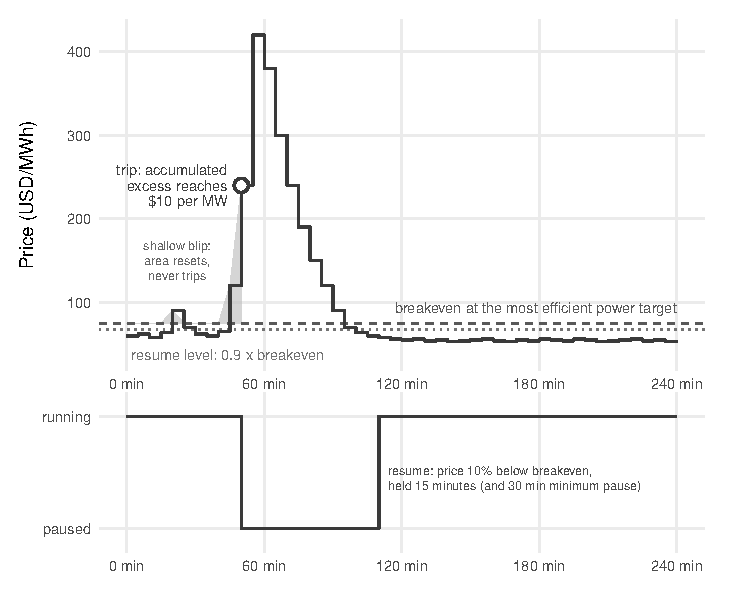
\includegraphics[width=\textwidth]{images/backstop}
  \caption{
    One backstop cycle, on an illustrative price trace. The shaded area is the trip statistic: price excess above the breakeven at the most efficient power target, integrated over time, reset whenever the price dips back below breakeven. Only sustained or very tall spikes pause the fleet. The trip, resume and minimum-time constants are the ones the backtests use. % fig-src: analysis/figures/fig_ch5_backstop.R (illustrative trace drawn with no feed lag; trip, resume and minimum-pause constants as analysis/ch5-backtest/papo_sim.py K_TRIP, RESTART_BAND, DWELL_S, MIN_DOWN_S, resuming on the third calm print as the kit does; console: trip at 50 min, restart at 110 min)
  }
  \label{fig:backstop}
\end{figure}

Resuming is deliberately asymmetric: the price must fall to 10~percent below breakeven and hold there for 15 minutes before the fleet comes back, and minimum runtimes of 30 minutes in each direction plus a budget of at most eight cycles per day cap the worst case. % src: analysis/ch5-backtest/papo_sim.py backstop constants, applied in simulate(): RESTART_BAND = 0.10 (resume needs p_prev <= be_val * 0.90), DWELL_S = 15*60 (held for 15 minutes of prints: three five-minute prints or one 15-minute print, t_prev - calm_since >= DWELL_S - sec), MIN_DOWN_S = MIN_UP_S = 30*60 (no resume within 30 min of a pause, no pause within 30 min of a resume), MAX_CYCLES_DAY = 8 (pauses per UTC calendar day; resumes are not budgeted, a detail left out of print per author 2026-08-28)
In thirty months of backtest across all eight ERCOT load zones the backstop tripped 0.12 to 0.53 times per day depending on the fleet and the zone, and adding the price deadband changed that count by exactly zero in every zone: modulation and pausing stay fully decoupled, as designed. % src: analysis/ch5-backtest/multizone_study.py summary (output/trend_study/multizone_rtm15.csv; 15-minute settlement prices, 2024-01-01 to 2026-06-23 UTC, 8 zones x 2 fleets): plain-hold backstop pauses 0.12 to 0.53 per day across the 16 cells and both windows; change in the pause COUNT with the deadband 0 in all 16 cells at every width from 10 to 40%, both windows

\section{Why There Is No Forecast}

The chapter's backtests compared sixty-seven alternatives to the last print, spanning slope extrapolation over 10-to-60-minute windows, exponential smoothing, rolling quantiles, and constant risk biases, and out of sample none of them beat it by anything worth building. On the S19j~Pro fleet nothing beat it at all; on the S21~XP three smoothing and rolling-quantile variants edged ahead by at most 0.2~percent of the plain hold's gain, under a dollar per machine in eighteen months. Across all eight load zones on the settlement point price, only the two gentlest slope settings, which barely extrapolate, came out ahead, by at most 0.12 percent; every other signal tested there lost in all sixteen zone-and-fleet combinations. % src: analysis/ch5-backtest/reactive_papo_trend.py summary (output/trend_study/sweep_results.csv; LZ_WEST five-minute prints, 30-minute hold, 67 signals plus persistence): TEST-2025-26 S19j Pro 0 of 67 beat persistence (best slope-ols W60 g5 -0.19% of the hold's uplift); S21 XP 3 of 67, ewma hl10 +0.16%, quant W15 q60 +0.13%, ewma hl15 +0.10% (counted on delta_pct; the summary once tested whole-dollar delta_vs_s14 and dropped wins under $0.50) (delta_vs_s14 $1, $1, $1 per machine over 538 days, whole dollars; ewma hl10's 0.16% of the hold's $542 uplift is about $0.87); on the S21 XP's 2,200 W best-point floor, until 2026-09-26, 5 of 67, best ewma hl10 +0.29%, about $1.57; no slope extrapolation beat it on either fleet; in sample (TUNE-2024) 6 and 9 smoothing or quantile variants did (6 on the S19j Pro in the committed CSV before and after the floor change; this comment said 5 until 2026-09-26). multizone_study.py summary (multizone_rtm15.csv), 7 representative signals: out of sample some signal beats persistence in 10 of 16 cells, only slope-ols W30 g5 and W60 g5, best +0.12%; the other five lose in all 16 (8 of 16 on the S21 XP's 2,200 W best-point floor, until 2026-09-26); in sample (TUNE-2024) bias +$10 also edges ahead in one cell, LZ_CPS S21 XP, by $0.06 (+0.01%), on the 2,774 W floor (behind in every cell on the 2,200 W one), hence no "ever" in the prose
The reason is structural, not a matter of tuning: because a big five-minute leap upward usually falls straight back, extrapolating a trend points the decision in exactly the wrong direction, and it is most wrong during spikes, when the stakes are highest.
Leaning the other way does little better. Out of sample, none of the six variants that push the decision price against every recent move beat the last print by more than 0.15 percent of the plain hold's gain, under a dollar per machine in eighteen months, and the two that push against falls but not rises, one of them extrapolating rises instead, lost on both fleets. On the 15-minute settlement point price in the eight load zones, none came out ahead at all. % src: analysis/ch5-backtest/fade_study.py --summary-only (output/trend_study/fade_study.csv; the eight fade signals of trend_followup.py EXTRA, decision price = last print + g x recent slope with g < 0, plain 30-min hold, delay 1, wins counted on the dollar delta to the cent): TEST-2025-26 LZ_WEST five-minute prints, rows equal to followup.csv; the six that fade every move (fade-end W15 and W30 at g -5 and -10, fade-ols W15 g-5, fade-ols W30 g-10) best fade-end W15 g-5 +0.15% of the hold's uplift, $0.81 per machine over 538 days (S21 XP), and fade-end W30 g-5 +0.15%, $0.50 (S19j Pro); the two fade-asym signals fade falls only (up0 dn-10) or fade falls and extrapolate rises (up15 dn-10), -0.22% and -1.90% (S21 XP), -0.64% and -2.72% (S19j Pro); deciding on the print and billing on the settlement point price at LZ_WEST, best +0.15% ($0.82) and +0.15% ($0.52); 15-minute settlement point price, 8 zones x 2 fleets, ahead in 0 of 16 cells, best -0.00% (-$0.02, fade-end W15 g-5, LZ_WEST S21 XP); on the S21 XP's 2,200 W best-point floor, until 2026-09-26, the S21 XP's best was +0.32% ($1.71) and 1 of 16 cells came out ahead by $0.02; worst -1.78% (-$3.81, fade-end W15 g-10, LZ_HOUSTON S19j Pro), largest dollar loss -$4.69 (-1.37%, same signal, LZ_WEST S19j Pro); at 15 minutes the W15 OLS-based signals, both fade-asym among them, equal persistence (two prices in the window) and fade-ols W30 g-10 equals fade-end W30 g-10 (three equally spaced prices), so four distinct signals are scored there; in sample (TUNE-2024) 6 of 8 on both fleets at five minutes, best +0.41% and +1.00%, 3 of 16 settlement cells, best +0.25%; two probes that fade rises only, not among the eight, best +0.31% ($1.71, S21 XP, five-minute prints), both lose on the S19j Pro, at most +0.08% in 7 of 16 settlement cells
These tests support persistence over the self-built signals tried here. They do not settle the make-or-buy question: no commercial forecast feed was tested. A paid feed would have to improve the loop's realized margin after its fee and the site's operating constraints, not merely predict prices more accurately.

\section{Two Prices, One Decision}

Chapter~3 left a subtlety that this loop has to respect: ERCOT bills a site on the 15-minute settlement point price, but publishes a fresh five-minute price three times per settlement interval. The loop decides on the five-minute print. Consumption is continuous, so a reaction to an interval's first print still changes the power drawn over the rest of that interval; the backtests, which let each print act only once its own five minutes are over, give it at most the remaining two-thirds. % src: arithmetic: SCED prices about every five minutes against 15-minute settlement intervals (ercot2026rtm), the settlement point price built from the interval's SCED LMPs (ercot2026protocols sec. 6.6.1), so three prints per interval; analysis/ch5-backtest/papo_sim.py load_mixed_basis bills each five-minute sub-interval at its interval's settlement point price, and simulate(delay=1) runs sub-interval i on print i-1, so the target set on the first print applies from the second sub-interval and carries into the third unless the second print moves it (mixed_basis_study.py docstring)
The catch the backtests exposed is that the fast feed and the price deadband work best together: under a plain 30-minute hold, five-sixths of the fresher prints arrive when the loop is not allowed to act. The fast feed alone adds little to what the plain hold earns over stock power (0.4~percent on the S21~XP fleet out of sample and 1.1~percent on the S19j~Pro; in 2024, the year that set the price deadband's width, it cost the S21~XP 0.8~percent). Together the two are worth more than the sum of their parts in all four window-and-fleet combinations the companion repository runs at LZ\_WEST. % src: analysis/ch5-backtest/output/trend_study/mixed_basis.csv, LZ_WEST, pct_of_s1 (capture) and vs_decide15_s14: TEST-2025-26 fast feed alone (decide-5 S14) 97.61 vs 97.23 (S21 XP), 93.85 vs 92.85 (S19j Pro), +0.38% / +1.07%; deadband alone (decide-15 +deadband10) +0.25% / +1.78%; together (decide-5 +deadband10) +0.86% / +3.66%. TUNE-2024 fast feed alone 94.34 vs 95.09 (S21 XP, -0.78%) and +1.06% (S19j Pro); deadband alone +0.31% / +2.35%; together +0.02% / +4.94%. Together exceeds the sum of the two alone in 4/4 cells
Speed pays on its own terms, too: every extra five minutes of feed latency costs the full loop about 0.8~percent of its gain over stock power on the S21~XP and 1.7~percent on the S19j~Pro, and a second five minutes costs about as much again, which makes fast ingestion part of the algorithm. % src: mixed_basis.csv TEST-2025-26 LZ_WEST, vs_full_loop of the full loop with one and two extra intervals of delay: decide-5 +deadband10 delay2 -0.76 (S21 XP) and -1.74 (S19j Pro); delay3 -1.48 and -3.66

One more reason the settlement point price matters: the adders. From half past five to a quarter past eight on the morning of January 13, 2025, LZ\_WEST's five-minute prints stayed below \$78, yet the settlement point price billed for those intervals reached \$187.77, 2.6 times the highest print in its interval; the difference was the reserve-scarcity adders of Chapter~3 riding on top. % src: analysis/checks/ch5_adder_example.py (LZ_WEST; MIS 13061 settlement vs NP6-788 prints): 2025-01-13 07:15 Central settled $187.77 on prints $71.16, $64.51, $71.62 (2.62x the highest); an unbroken run of 7 intervals, 06:30 to 08:15 Central, settled $115.59 to $187.77 while no print from 05:30 to the run's last, 08:10, exceeded $77.68 (the day's next print above it, $84.12, came at 17:35 Central). Replaces the $1,629.89 of 2025-06-30, a corrupted row of the legacy cache (ERCOT's archive has $34.17)
A loop deciding on bare five-minute prints would have hashed straight through. On that day's hashprice an S19j~Pro loses money above \$96 even at its most efficient point, so for an hour and three-quarters an S19j~Pro fleet ran at a loss that no print revealed. % src: ch5_adder_example.py: hashprice $0.0550/TH/day on 2025-01-13 (analysis/data/hashprice_daily.csv); S19j Pro best-point breakeven $96.21 (41,666.7 x hashprice / 23.83 J/TH), stock $77.72; every print below it and every settlement of the run above it. For the S21 XP (breakeven $184.27 at its most efficient power target, 3,200 W, 12.44 J/TH, the best efficiency in the loop's range; $184.95 at its 2,200 W best point, the floor until 2026-09-26) only 1 of the 7 intervals settled above breakeven, so the claim is made for the S19j Pro
The reliability-deployment adder adjusts prices for the effect of ERCOT's interventions to keep the grid reliable. The example predates RTC+B, which on December 5, 2025 retired the ORDC adder and moved scarcity pricing into the energy price itself (Section~\ref{sec:rtcb}); the reliability-deployment adder remains, so the bill can still run ahead of the prints: on March 23, 2026, LZ\_WEST settled at \$950.48 in an interval whose highest print was \$758.06 \autocite{ercot2025rtcblive,potomac2026somercot,ercot2026protocols}. % src: analysis/checks/ch5_adder_example.py console, "largest settlement above the highest print after RTC+B: 2026-03-23 21:45 Central, settled $950.48 on a highest print of $758.06" % src: ercot2025rtcblive (go-live Dec 5, 2025); potomac2026somercot p. 2 (ORDC adder "discontinued in December 2025 with the introduction of RTC"; shortage pricing "incorporated into the price of energy rather than functioning as a separate adder"), as chapter-3 sec:rtcb; ercot2026protocols sec. 6.6.1 (current Real-Time Settlement Point Price includes the reliability-deployment adder). ch5_adder_example.py: LZ_WEST intervals settled at $100 or more and above 1.5x their highest print, 26 from Dec 2023 to Dec 4, 2025, none from Dec 5, 2025 to June 22, 2026; mean |settlement - mean print| $0.617 before, $0.450 after
That is why the ladder of Figure~\ref{fig:oracle-benchmark} and the price deadband, latency and zone results in this chapter score the loop at the 15-minute settlement point price, never at the print it saw.

\section{The Report Card: Chasing the Oracle}
\label{sec:oracle}

The benchmark is an \glossaryterm{oracle}{oracle}: a hypothetical operator with perfect foresight and zero friction. Concretely, in every interval the oracle sets the machine to the profit-optimal power for that interval's own settlement point price, a price no one can know until after the interval has ended, and it pauses for free whenever even that optimum would lose money: no hold, no price deadband, no minimum runtimes, no resume ramp, no publication delay. % src: papo_sim.py, signal='S1' ("perfect foresight, free pause, no hold, no backstop"); optimal_power(current interval's settle price), profit floored at 0 by the free pause
The oracle is a ceiling on what responding to the energy price can earn, not a strategy; nothing real sees the future. One number grades every real configuration against it: \glossaryterm{capture}{capture}, the share of the oracle's gain that a real strategy earns over the same intervals, where the gain is profit above simply running every machine at stock power and never pausing. Chapter~\ref{ch:stack} reuses the ratio against benchmarks of its own, not this oracle. % src: analysis/ch5-backtest/mixed_basis_study.py, pct_of_s1 = (strategy - S0) / (S1 - S0), S0 = default (stock) power in every interval, never paused (papo_sim.py signal=None); the oracle prices energy only (papo_sim.py profit(): hashprice revenue less energy at the settlement point price), so it is no ceiling on the transmission charge chapter 8 prices; chapter 9 reuses the ratio form, gain over never pausing, but against its own stock-power, pause-only twin, not this oracle: analysis/checks/ch9_flexibility_stack.R capture = gain_lag / gain_fc, gain_fc = sum(pmax(P - V, 0)) * E, the foresight pause at stock power and nameplate J/TH (jth 29.5 and 13.5), with gain_lag deciding on p_lag, the previous 15-minute settlement price (or the day-ahead price on the day-ahead index); chapter 9 also grades its planned site by capture against the hindsight ceiling of its annual switches, which is no twin (analysis/checks/ch9_optimal_stack.R CAPTURE line, chapter-9.tex:175)
The shortfall is not all blindness. Out of sample, two-fifths to half of it is the cost of the loop's own rules (the hold, the price deadband, the backstop and the minimum runtimes), and most of the rest is that no five-minute print reveals the settlement point price the interval will be billed at. % src: analysis/ch5-backtest/capture_anatomy.py console, TEST-2025-26, "INFO shortfall ... = information ... + friction": S21 XP 1.93 = information 0.97 (basis 0.71 + latency 0.27) + friction 0.96, S19j Pro 3.75 = 2.19 (1.49 + 0.70) + 1.56; friction, the loop's own rules (hold, price deadband, backstop, runtimes), is 0.96 / 1.93 = 50% and 1.56 / 3.75 = 42% of the shortfall; basis, no print reveals the settlement point price, is 0.71 / 0.97 = 73% and 1.49 / 2.19 = 68% of the rest; "INFO frictionless causal loop" 99.03 / 97.81 deciding on print i-1 and 99.29 / 98.51 on the current print; the split is sequential (basis, then latency, friction as what remains), one attribution of several (capture_anatomy.py docstring); in 2024 friction is 2.41 of 4.89 and 1.62 of 7.20, hence "out of sample"
Figure~\ref{fig:oracle-benchmark} places the four real configurations against the oracle, out of sample at LZ\_WEST, settled on the 15-minute settlement point price.

\begin{figure}[htbp]
  \centering
  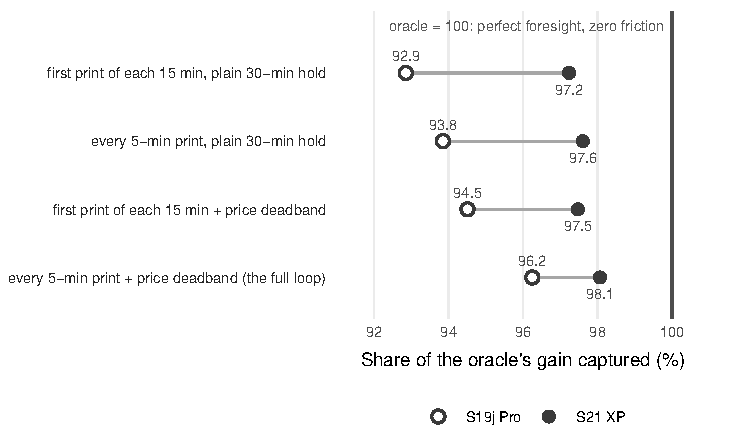
\includegraphics[width=\textwidth]{images/oracle_benchmark}
  \caption{
    Share of the oracle's gain captured by four real configurations at LZ\_WEST, out of sample, for the two fleets of Chapter~4; the gain is profit above running at stock power without ever pausing. The fast feed alone and the price deadband alone each buy little; together they capture 98.1~percent (S21~XP) and 96.2~percent (S19j~Pro) of what perfect foresight gains. Settled on the 15-minute settlement point price, with power curves from the 2026-Q2 fleet data. % fig-src: analysis/figures/fig_ch5_oracle_benchmark.R, which reads analysis/ch5-backtest/output/trend_study/mixed_basis.csv (window TEST-2025-26, zone LZ_WEST, deadband 10 percent of default power; pct_of_s1 98.0661 and 96.2485) and prints the window: 154,975 paired 5-minute intervals, 2025-01-01T00:00Z to 2026-06-23T04:55Z (538 days, to June 22, 2026 Central), out of sample for the price deadband's width, set on 2024; backstop constants: analysis/ch5-backtest/README.md and papo_sim.py provenance note. Billed on ERCOT MIS 13061 settlement point prices, decided on the NP6-788 five-minute prints. The engine runs the 2026-Q2 fleet telemetry curves Figure 5.1 draws, with the modulation floors of telemetry_miner.py modulation_floor: 1,200 W, the S19j Pro's best-efficiency point, and 2,774 W, the S21 XP's Braiins OS default minimum (98.1805 for the S21 XP on its 2,200 W best point, the floor until 2026-09-26). Was 97.6/94.8 on 136,783 intervals to April 2026, from a legacy price cache with a corrupted row
  }
  \label{fig:oracle-benchmark}
\end{figure}

At LZ\_WEST the full loop, five-minute feed plus price deadband plus backstop, captures 95 to 98~percent of what perfect foresight would gain on the newer fleet and 93 to 96~percent on the older one, the lower figures in 2024 and the higher out of sample. % src: analysis/ch5-backtest/output/trend_study/mixed_basis.csv, zone LZ_WEST only, variant decide-5 +deadband10, pct_of_s1 across both windows: S21 XP 95.11 (tune 2024) and 98.07 (test 2025-26), S19j Pro 92.80 and 96.25. The four configurations of Figure 5.5 fall between 88.43 and 98.07 in the two windows
The result is out of sample for only one setting, the price deadband's width, which was set on 2024's prices. The backstop's settings come from an earlier Braiins study whose price record ran from December 2023 to June 2026, and the loop's design itself, deciding on the last print every five minutes under a 30-minute hold, from earlier Braiins backtests on prices that overlap this window. Choosing the backstop's settings on 2024 alone instead moves the out-of-sample result by less than half a point; the design itself was not re-chosen that way. % src: analysis/ch5-backtest/papo_sim.py, provenance note above K_TRIP, and README.md "Provenance of the constants": K_TRIP, RESTART_BAND and DWELL_S (with the runtimes and the cycle budget) come from an earlier Braiins backstop study whose grid search ran on LZ_WEST five-minute prints from 2023-12-11 to 2026-06-23; the price deadband's width, 10% of stock power, is the only setting chosen on TUNE-2024; the loop's design (persistence every five minutes, the 30-minute hold) comes from earlier Braiins work whose backtests overlap TEST-2025-26; capture_anatomy.py console "RETUNE TUNE-2024 pick" (18 settings, K_TRIP 5/10/20 x RESTART_BAND 0/0.05/0.10 x DWELL 15/30 min, best TUNE-2024 capture of the full loop): S21 XP picks K_TRIP 20, band 0.05, dwell 15 (TUNE-2024 95.66 against the printed setting's 95.11, rank 6 of 18), TEST-2025-26 97.86 against 98.07, -0.21 points; S19j Pro picks the printed setting (rank 1), +0.00; "RETUNE all 18 settings on TEST-2025-26, minus the printed setting" -0.86 to +0.05 and -1.16 to +0.29, so "less than half a point" is the 2024 pick's, not every setting's; nothing in the kit re-selects the loop's design on TUNE-2024 alone (papo_sim.py note, README.md), hence "not re-chosen that way"
A strategy with no forecast, no vendor data, and hardware-friendly actuation leaves single-digit percent on the table against perfect foresight. The run-or-pause call is rarely in doubt: in 2025, about 86 percent of LZ\_WEST's five-minute intervals sat below even the stock S19j~Pro's breakeven, where both fleets should run. % src: analysis/checks/ch5_oracle_check.R on analysis/data/ercot_spp_rtm5_lzwest.csv.gz filtered to 2025: 86.5% of 2025 LZ_WEST 5-min intervals below the stock S19j Pro breakeven at the 2025-mean hashprice; below it stock power makes money on both fleets, so the oracle runs (the S21 XP's breakevens are higher: papo_sim.py check_breakevens, 148/144 against 77/65 $/MWh at best point / stock, $44.31/PH/day); ch5_oracle_check.R's oracle pauses at stock power only and decides and bills on the same five-minute print, so its 94.1% for a 1-interval-lag pause-only rule (99.1% of that oracle's profit, always-on 84.3%) is a share of a smaller, pause-only gain, not Figure 5.5's yardstick; against Figure 5.5's oracle, which also moves the power target, pausing alone at stock power takes 22 and 65% (analysis/ch5-backtest/baselines_study.py), as the next paragraph prints
The oracle still pulls ahead in those intervals, through the power target and through how soon the loop resumes after a pause, but the price level persists, so the target the last print points to is usually the one the oracle would have set. % src: analysis/ch5-backtest/capture_anatomy.py console, TEST-2025-26, "SAME-TARGET steps in which the target computed from print i-1 equals the oracle's" (the profit-optimal power target at the previous print, or a pause where even that loses money, against the oracle's on the step itself; a pause counts as a target): 98.85% (S21 XP) and 88.37% (S19j Pro), 99.02 and 88.32 over the oracle's running steps only (2024 98.79 and 89.96); "SAME-TARGET steps at or below the stock S19j Pro breakeven", the counterpart over the whole TEST-2025-26 window, on Figure 5.5's settlement point price, of the 2025 86 percent above: 86.06% of steps, holding 71.63% and 25.77% of the oracle's gain and 16.37% and 38.28% of the full loop's shortfall, the loop paused in 47 and 511 of them, still waiting out the backstop's resume rule
Pausing is where a loop that reacts one print late should lose most, and counted interval by interval it does. Out of sample it is paused in only 79 and 67~percent of the intervals in which the oracle pauses, on the S21~XP and the S19j~Pro. % src: analysis/ch5-backtest/capture_anatomy.py console, TEST-2025-26, "RECON oracle-pause steps in which the full loop is also paused, by count": 78.53% (2,297 of 2,925, S21 XP) and 67.29% (9,033 of 13,424, S19j Pro); 2024 67.20 and 60.10; the oracle pauses in 1.89% and 8.66% of the window's five-minute steps ("RECON oracle pauses in ... steps")
In dollars, though, it recovers 96 and 97~percent of what the oracle's pausing earns. The intervals it misses hold only 5 and 11~percent of that value, and through them the S19j~Pro still turns down, mostly to its floor, which wins back three-quarters of what they are worth. % src: capture_anatomy.py console, TEST-2025-26, "RECON the full loop's recovery of the pause class's gain, in dollars": 96.34% and 97.19% (2024 91.66 and 94.33) of the pause class, the oracle-paused steps, which hold 24.26% and 69.36% of the oracle's gain; of which by being paused 95.45 and 88.57, the rest, net, by running below stock power through those steps, mostly at the floor ("RECON the rest of that recovery ... by applied target": floor +0.58 and +6.47, other targets below stock +0.39 and +2.17, stock power and above -0.10 and -0.02); the steps the loop misses hold 100 - 95.45 = 4.55% and 100 - 88.57 = 11.43% of the pause class's gain, and running through them wins back 96.34 - 95.45 = 0.88 and 97.19 - 88.57 = 8.62, so 8.62 / 11.43 = 75% on the S19j Pro, the floor 6.47 of the 8.62 (0.88 / 4.55 = 19% on the S21 XP); in 2024 the missed steps hold 8.76% and 13.42%, and the S19j Pro wins back 7.75 of its 13.42, 58%
Episodes of more than three hours above breakeven hold about four-fifths of that value, and the loop recovers 99~percent of it. The episodes it handles worst last an hour or less; they are seven in ten of all episodes but hold under a tenth of the value. % src: capture_anatomy.py console, TEST-2025-26, "RECON episodes" (runs of contiguous oracle-paused steps; 155 and 798 episodes): longer than 3 h 14.2% and 10.9% of the episodes, 83.6% and 79.3% of the pause class's gain, recovered at 99.4% and 99.3%; 1 to 3 h 16.8% and 17.3%, 10.1% and 12.1% of the gain, 92.8% and 92.5%; 1 h or less 69.0% and 71.8% of the episodes, 6.3% and 8.6% of the gain, recovered at 61.6% and 84.2%, the lowest; out of sample only: in 2024 episodes over 3 h hold 33.0% and 42.6% of the gain
Leaps far past breakeven usually start falling back at once. LZ\_WEST's price jumped \$100 or more in a single print 555 times from 2024 to mid-2026, about once every 1.6 days, and seven times in ten the very next print was lower. The backstop caps how long any of them can hurt. % src: analysis/checks/ch5_price_autocorrelation.py, first two console lines, LZ_WEST five-minute prints 2024-01-01..2026-06-22 Central (904 days): after rises of $100 or more n=555 (one per 1.6 days), next print lower 69% of the time; after falls of $100 or more it kept falling 71% of the time (one-sided reversion, as line 43 says)

Two baselines give the loop's capture its scale. Never pausing at stock power already earns 90 percent of the oracle's profit on the S21~XP and 75 percent on the S19j~Pro, out of sample and before pool fees, the Braiins~OS development fee (Section~\ref{sec:stack-power-target}) and grid charges. Pausing alone, the backstop at stock power, closes 22 and 65 percent of the remaining gap, and even perfect foresight at stock power, the strike of Chapter~\ref{ch:buying}, would close only 24 and 73 percent. % src: analysis/ch5-backtest/baselines_study.py (output/trend_study/baselines.csv), TEST-2025-26, LZ_WEST, 154,975 paired intervals, Figure 5.5's engine and billing: S0 / S1 profit per machine 5,121.33 / 5,681.21 = 90.1% (S21 XP) and 1,090.76 / 1,458.60 = 74.8% (S19j Pro); both are gross: papo_sim.py and telemetry_miner.py profit() is A*H(p) - B*p, the day's hashprice on the hashrate less the settlement point price on the power, with no pool fee, no Braiins OS development fee (defined in chapter 9 sec:stack-power-target) and no grid charge; backstop alone at stock (floor = ceiling = stock power, stock breakeven, papo_sim.py backstop constants) 22.30% and 65.32% of S1's gain, 0.18 and 0.69 pauses a day; S1 at stock 24.28% and 72.52%; the stock oracle is chapter 6's strike rule on each day's hashprice: over calendar 2025 it is worth $17,636 and $48,945 per MW-year of stock draw, against fig_ch6_strike.R's $17,280 and $49,116 (asserted within 2.5%); on/off at every print at stock, no hold, minimum runtime or cycle budget, 23.39% and 70.40% at 1.3 and 8.1 switches a day; TUNE-2024: always-on 90.7% and 84.7%, backstop alone 14.15% and 47.30%, stock oracle 18.72% and 56.86%; S0, S1 and full-loop rows asserted equal to mixed_basis.csv
The rest is the curve: on the S21~XP almost all of it is running above stock power in cheap intervals, which a site can do only where its connection has room (Section~\ref{sec:stack-power-target}). % src: baselines_study.py TEST-2025-26 LZ_WEST: full loop with its ceiling held at stock 22.65% (S21 XP) and 75.30% (S19j Pro) (console row "full loop, ceiling at stock"; 22.02% and 74.92% before the 2026-10-03 telemetry_miner.scan_powers fix, on the 10 W grid that could not reach 3,645 or 3,068 W; 2024 14.16% and 53.73%), with its floor raised to stock 97.52% and 86.27%, full loop 98.07% and 96.25%; chapter-9.tex sec:stack-power-target (the connection binds: the S21 XP pins at its ceiling and the S19j Pro is held below stock under a 67.13 MW connection)
Given that room, a fixed power target at the S21~XP's 3,990~W ceiling, with the same backstop and no price-following at all, already captures 97.6~percent, so the newer fleet's score mostly grades a setting, not the reflex. On the S19j~Pro a fixed target at its own 3,420~W ceiling captures only 77~percent, and the reflex lifts it to 96. % src: analysis/ch5-backtest/baselines_study.py console row "ceiling + backstop" (output/trend_study/baselines.csv), TEST-2025-26 LZ_WEST: every machine fixed at its power ceiling, 3,990 W (S21 XP) and 3,420 W (S19j Pro), never moved (papo_sim.py simulate(fixed_power=p_max)), paused only by the loop's own backstop at the curve's best-point breakeven, 97.6069% and 77.3556% of the oracle's gain against the full loop's 98.07% and 96.25% (2024 94.93% and 82.70% against 95.11% and 92.80%); with the backstop at the ceiling point's own breakeven instead ("ceiling + backstop (own breakeven)") 97.6172% and 83.1285% (2024 94.867% and 84.5972%)

Call the weakest configuration of Figure~\ref{fig:oracle-benchmark} the naive design: one five-minute print every fifteen minutes (the first of each settlement interval), each power target held at least thirty minutes, the same backstop, and no price deadband. Out of sample at LZ\_WEST, at each day's own hashprice, which averaged about \$0.045 per terahash-day, the full loop earns about \$3,200 a year more than the naive design per thousand S21 XPs, and about \$8,500 more per thousand S19j Pros, some \$900 and \$2,800 a year per megawatt of stock draw. The 30-minute hold alone cuts the S19j~Pro's target moves to under half of retargeting on every print, 13 a day against 32, and the price deadband wins back nearly all of the value the hold gave up, 97 percent of it, with about four-fifths as many moves as retargeting on every print. % src: analysis/ch5-backtest/naive_gap.py (output/trend_study/naive_gap.csv), TEST-2025-26, LZ_WEST, 154,975 paired intervals, 538.2 days: naive design = decide-15 S14, the weakest of Figure 5.5's four out of sample on both fleets (capture 97.23 and 92.85; the hold is a minimum dwell of 1,800 s); full loop = decide-5 +deadband10; full_minus_variant $4.66 (S21 XP) and $12.49 (S19j Pro) per machine, usd_per_year_per_1000 3,158 and 8,469, usd_per_mw_year 866 and 2,760 (3,158 / 3.645 MW and 8,469 / 3.068 MW of stock draw); hashprice console line: the kit's hashprice_daily.csv averages $45.41/PH/day ($0.0454/TH/day) over the paired intervals, the book's Braiins Insights series (analysis/data/hashprice_daily.csv) $45.46 on the same intervals, no day of the window more than $3.77/PH/day apart (2025-11-13 to 15 are absent from the kit's file and carried from the day before) (TUNE-2024 120 and 12,485; against the fast-feed plain hold decide-5 S14, 1,750 and 5,984; the S21 XP's 3,950 was on its 2,200 W best-point floor, until 2026-09-26); S19j Pro changes_day decide-5 S14 13.4, decide-5 every print 32.0, full loop 26.3, 26.3/32.0 = 82%; console fast-feed line: the price deadband wins back 97.3% (S19j Pro) and 98.5% (S21 XP) of what the plain hold gives up against every-print retargeting, which earns 164 and 27 dollars a year per 1,000 more than the full loop; rows shared with mixed_basis.csv asserted equal; the naive design's slow feed is the print stamped at the start of each 15-minute settlement interval, carried for its three steps (mixed_basis_study.py coarsen(), t % 900 == 0), not the settlement point price
Notice who benefits most: the S19j~Pro gains more from every rule than the S21~XP does. That is Chapter~4's operating leverage again, seen from the control room; the closer a machine lives to its breakeven, the more each percentage point of price discipline is worth. The marginal machine needs the reflex most.

Every capture in this chapter charges nothing for a move; the backtest applies each new power target at once, at full efficiency. % src: analysis/ch5-backtest/papo_sim.py simulate() defaults move_loss_s=0 and first_visit_s=0, which every capture in this chapter was computed with: once the hold or the price deadband allows it, the new target applies within the interval and profit is booked at full curve efficiency (README.md, The engine)
Because each target is tuned once and later visits reuse its saved profile, leaving that out costs little. Even three hours of settling on each target's first visit takes under a point off either fleet's capture out of sample. % src: analysis/ch5-backtest/capture_anatomy.py console, TEST-2025-26, "MOVES saved-profile model" (simulate(first_visit_s=...): zero hashing at full draw the first time in a run the loop applies each of its 4 and 8 targets, later visits free): full loop at 10,800 s per first visit 97.17% (S21 XP) and 95.39% (S19j Pro) against 98.07% and 96.25%, -0.90 and -0.86 points; at 600 s 97.99% and 96.18%; 2024 at 10,800 s 93.32% and 90.44% against 95.11% and 92.80%, hence "out of sample"
A cost per move would matter more. Every second of hashing lost per move takes about 0.2 points off the S19j~Pro's capture and about 0.03 off the S21~XP's; the S19j~Pro moves its target about 27 times a day, counting resumes, and the S21~XP under three times. At about 26 seconds a move, the price deadband would stop paying for its extra moves on the S19j~Pro. % src: analysis/ch5-backtest/capture_anatomy.py console, TEST-2025-26, "MOVES decide-5 +deadband10" (simulate(move_loss_s=...): every physical power-target change, a move the hold or the price deadband allows or the target set at a backstop resume, costs that many seconds of hashing with the power still billed): 26.85 physical moves a day (26.34 + 0.51 resumes, S19j Pro) and 2.59 (2.42 + 0.17, S21 XP); 0.1882 and 0.0345 capture points per second (2024 0.2000 and 0.0356); capture at 30 s 90.60% and 97.03%; "MOVES full loop stops beating decide-5 S14 at" 26.3 s (S19j Pro; 2024 29.5 s), the plain hold on the same five-minute feed, the full loop without its price deadband (43.1 s on the S21 XP); against the naive design ("stops beating decide-15 S14 at") 33.4 s and 55.2 s; the per-move cost is a sensitivity, not a measured firmware figure

The design work behind this chapter is Braiins' own, and it is published here for the first time. Everything else in this paragraph you can rerun yourself from the companion repository. It recomputes the ladder above on ERCOT's own published prices and on the same fleet curves Figure~\ref{fig:efficiency-curves} draws. It shows the price deadband beating the plain hold in all sixteen zone-and-fleet combinations, in 2024 and again in January 2025 through June 2026, at each of the three widths tried from 10 to 25~percent. So the result does not hang on where the width was set. At the fourth, 40~percent, it never fires on the S21~XP, whose whole power range is narrower than that, and there it only ties the plain hold. And it checks the optimizer that picks each power target against an exhaustive search over every operating point between each curve's floor and ceiling. The check uses about 250,000 ERCOT price observations: a sample of 200,000 positive prices plus all 50,000 zero or negative prices in LZ\_WEST's five-minute prints and the eight load zones' 15-minute settlement prices, from January 2024 through June 2026. The two methods pick the same target every time. % src: ladder: analysis/ch5-backtest/mixed_basis_study.py (output/trend_study/mixed_basis.csv); price deadband: analysis/ch5-backtest/multizone_study.py --all-zones summary (DEADBANDS 0.10, 0.15, 0.25, 0.40; output/trend_study/multizone_rtm15.csv): uplift above the plain hold in 16/16 cells at 10, 15 and 25% in TUNE-2024 and in TEST-2025-26, and in 8/16 at 40%, where the 8 S21 XP cells equal the plain hold exactly (delta_vs_s14 0.0: 40% of 3,645 W is 1,458 W, more than the 1,216 W between the 2,774 W floor and the 3,990 W ceiling, so the deadband cannot fire; 16/16 at all four widths on the 2,200 W best-point floor, until 2026-09-26), pause count unchanged; re-run 2026-09-26 on the S21 XP's 2,774 W floor; optimizer: analysis/ch5-backtest/optimizer_bruteforce_check.py summary (output/trend_study/optimizer_bruteforce.csv): 250,214 real prices 2024-01-01 to 2026-06-24 UTC, 124,745 LZ_WEST NP6-788 prints and 125,469 MIS 13061 settlement point prices over 8 zones, a seeded sample of 100,000 positive prices per series plus every price at or below zero in both series, 50,214 of them (low -228.75 $/MWh), so the sample over-weights them; candidates are the measured points between each curve's floor and ceiling plus the interpolated ends of the range (the 3,420 and 3,990 W ceilings and the S21 XP's 2,774 W floor); same power target in 500,428 of 500,428 choices over both fleets, largest shortfall 0.00 $/machine-hour, 0 run-or-pause disagreements; a deliberately broken 50 W scan fails the same check; "published here for the first time" per author request 2026-08-27
None of this is a field result. The loop's numbers are backtests on ERCOT's published prices and fleet-average curves, so that a reader can rerun them; the book's field evidence of what pausing earns is what Riot, a listed miner, reports (Chapters~2, 3 and~6). % src: analysis/ch5-backtest (mixed_basis_study.py, baselines_study.py and naive_gap.py on ERCOT MIS 13061 settlement point prices and NP6-788 LZ_WEST prints, with the fleet-average curves of analysis/data/miner_efficiency_telemetry_2026q2.csv); the kit replays no site's own record; field evidence: chapter-2.tex:106 (Riot2024Jan, Riot2025Jan: curtailment and demand-response credits), chapter-3.tex:132 (August 2023 resale and demand response), chapter-6.tex:83 and :136 (riot10k2025, riot10k2024 power curtailment credits); ERCOT's own measurements of the mining response, chapter-3.tex:124 (about 4,100 MW of Winter Storm Fern curtailment credited to miners) and chapter-8.tex:88 (about 3,150 MW cut on August 18, 2025), are megawatts, not what the pauses earned

Price Adapt in Braiins Manager, the fleet software I work on at Braiins, implements the loop. It uses electricity prices, hashprice and the machine's efficiency curve to choose the most profitable power target, or a pause when running does not pay. Braiins~OS autotuning puts the chosen target into practice by adjusting each chip's voltage and frequency \autocite{braiinsacademypriceadapt,braiinsacademyautotuning}. % src: braiinsacademypriceadapt, read 2026-09-25: Price Adapt uses Day-Ahead Market (DAM) pricing and a daily planning cycle builds the next day's plan; for each hour it evaluates each miner model's efficiency curve against energy price and hashprice and selects the power setting with the highest hourly net profit; if no setting is profitable the miner is curtailed (paused) for that hour; power-target changes on supported Braiins OS models, pause and resume only on stock firmware; profile field Tolerance (USD/MWh) shifts the profitability threshold for both curtailment and power-target decisions; ERCOT and PJM day-ahead prices; currently under active development
% Historical provenance (detail removed from prose on 2026-10-02): Braiins Academy Continuous Tuning page, read 2026-09-25 (page titled Continuous Tuning (beta); an advanced autotuning mode, enabled in Advanced Settings, that replaces the one-off tune; every tuning cycle, approximately 5 minutes, recalculates frequencies and voltages for current conditions; the About page says every few minutes); Braiins OS release notes, release 26.04 dated April 15, 2026: continuous tuner in official beta, still beta through 26.09.1 of September 24, 2026; how it reaches a new power target is stated on no public Braiins page checked, so nothing is printed about it

And with that, the reflex is done. Capture in the nineties means the remaining money is not in better reflexes. It is in two places this loop cannot reach: buying the electricity better in the first place, which is Chapter~6's contract menu and strike price, and getting paid for the readiness itself, which is what ERCOT's ancillary services buy and Chapters~7 through 9 price. The machine can now flex. The rest of this book is about selling it.


\part{Monetizing Flexibility in ERCOT}

\chapter{Buying Power: Contracts, Price Arbitrage, and the Strike Price}
\chaptermark{Buying Power}
\label{ch:buying}

Chapter~5 built a machine that flinches away from expensive electricity in minutes. This chapter asks the question that the machine cannot answer for itself: expensive compared to what? The answer is written in a contract. Two mining sites in the same county, drawing the same megawatts through the same weather, can end the year with wildly different power bills because one signed a fixed price in 2021 and the other buys every fifteen minutes at whatever the market says. Before the book can price flexibility, it has to price the electricity, and electricity is not bought at ``the market price.'' It is bought through one of a small menu of contract shapes, and the shape decides what you pay on an average day, what you pay in a crisis, and whether your off switch is connected to anything at all.

\section{The Contract Menu}

Every power contract is an answer to one question: who carries the price risk. At one end of the menu sits the \glossaryterm{power-purchase-agreement}{power purchase agreement} (PPA), a bilateral contract that fixes the volume, price and term of the power bought; the supplier carries the market risk, and charges for the service. At the other end sits the \glossaryterm{index-contract}{index contract}, where the buyer pays the market's settlement price for every interval it consumes; the buyer carries everything. In between sit \glossaryterm{block}{blocks}: fixed prices for fixed slices of the week, hedging some hours and leaving the rest exposed.

These contracts are all on the books of publicly traded Bitcoin miners in Texas, disclosed in enough detail to study because United States securities law makes large companies file their material contracts.

Riot Platforms runs its Rockdale facility, one of the largest Bitcoin mines in the world, on the fixed end of the menu: 345~MW of long-term fixed-price power, contracted in three tranches between May 2020 and November 2022, at fixed prices running to April 2030 for the first two tranches and October 2027 for the third \autocite{riot10k2024}. % src: riot10k2024, Note 20 (130 MW May 2020 + 65 MW Mar 2022 to Apr 2030; 150 MW Nov 2022 to Oct 2027)
The same contract contains the clause this whole book turns on: Riot may elect \emph{not} to consume its fixed-price power and instead sell it back, taking credits against future power bills whenever the spot price makes that the better trade. % src: riot10k2024, Note 20 sell-back election
Hold that clause; Section~\ref{sec:arbitrage} is about what it is worth.

Cipher Mining's Odessa facility sits nearby on the menu: a PPA with Luminant at approximately 2.7 cents per kilowatt-hour, which is \$27/MWh in this book's units, running to at least July 2027 \autocite{cipher10k2024}. % src: cipher10k2024, Luminant Power Agreement ("approximately 2.7 c/kWh")
It is a \glossaryterm{take-or-pay}{take-or-pay} contract: Cipher must accept and pay for at least 66.7~percent of the site's 207~MW capacity every year whether it consumes the power or not. % src: cipher10k2024 (66.7% of 207 MW, take-or-pay)
Like Riot, Cipher can route unneeded power back to the market through its supplier; those power sales brought in \$5.4~million in 2024 and \$9.9~million in 2023. % src: cipher10k2024, power sales proceeds
Cipher's other Texas sites, Bear and Chief, have no fixed-price contract at all: they buy at the spot price and manage cost purely by pausing when prices are high. % src: cipher10k2024 ("do not currently have fixed price power purchase agreements"; curtailment software)

IREN went furthest toward the bare end. In August 2024 it paid \$7.2~million to close out its remaining hedges and moved its Childress site to buying directly from the ERCOT wholesale spot market \autocite{iren10k2025}. % src: iren10k2025, Item 1 (hedge close-out, spot participation from August 2024)
Its own filing states the flip side plainly: IREN warns its investors that on the spot market it may not be able to curtail when prices are high, in particular for the AI and high-performance-computing loads it also hosts, because those customers require uptime. % src: iren10k2025, Risk Factors, "We may be affected by price fluctuations in the wholesale and retail power markets" (about p. 44), verbatim, read at EDGAR 2026-10-03: "Further, if we purchase our electricity from the ERCOT spot market, we may not be able to curtail our operations when prices are high (in particular, we may not be able to curtail our operations relating to the delivery of HPC and AI services due to customer expectations or requirements relating to uptime), and even if we do curtail the electricity prices may remain high for a long period, meaning our operations are curtailed for extended periods of time"; until 2026-10-03 the prose opened with "a spot buyer can escape high prices only by pausing consumption", the author's inference, dropped because the sentence attributes it to the filing
The spot market is a dangerous place for a load that cannot stop, and a reasonable one for a load that can.

Between fixed and spot sit the standard block shapes, and they have exact definitions because they trade as futures contracts. \glossaryterm{on-peak}{On-peak}, written \glossaryterm{on-peak}{5x16}, covers the sixteen hours from 6~a.m.\ to 10~p.m.\ Central time (the market labels each hour by when it ends, HE~7 through HE~22), Monday through Friday, excluding six market holidays \autocite{ice2026ercotnorthpeak}. % src: ice2026ercotnorthpeak (HE 0700-2200 CPT, Mon-Fri ex NERC holidays)
\glossaryterm{off-peak-nights}{Off-peak nights}, written \glossaryterm{off-peak-nights}{7x8}, covers the other eight hours of every day; \glossaryterm{2x16}{2x16} covers the same sixteen hours on Saturdays, Sundays and those six holidays; the three tile the week, and 7x24 is around the clock \autocite{ice2026ercotnorth7x8,ice2026ercotnorth2x16}. % src: ice2026ercotnorth7x8 (HE 0100-0600, 2300-2400 all days); ice2026ercotnorth2x16 (each Saturday, Sunday and all NERC holidays, HE 0700-2200 CPT); the three tile the week: 5x16 and 2x16 split HE 0700-2200 of every day between them, 7x8 takes the other eight hours; 7x24 follows arithmetically
A miner quoted ``forty-two dollars for calendar-26 5x16'' is being offered a fixed price for exactly that slice of next year. One caution travels with every block quote: the futures settle at trading hubs, while a mine pays its own load zone's price, and the gap between the two, called \glossaryterm{basis}{basis}, is a risk the block does not cover.
At LZ\_WEST it is not small: across all hours the zone averaged about \$10/MWh above the North hub in 2023, 2024 and 2025, more than the whole non-energy stack of Table~\ref{tab:btm-ledger}, and within \$2 of the hub in 2021, 2022 and 2026 so far; inside the 5x16 window the three large gaps were \$5 to \$7. % src: analysis/checks/ch6_basis.R console (MIS 13061 15-minute settlement prices, LZ_WEST minus HB_NORTH, all hours: 2021 -1.60, 2022 +0.20, 2023 +11.12, 2024 +9.82, 2025 +10.16, 2026-01-01 to 08-29 +0.35; 5x16 window, NERC holidays excluded: 2021 -2.33, 2022 -0.22, 2023 +6.63, 2024 +6.46, 2025 +5.11, 2026 -2.43, so the stack comparison holds across all hours only; stack 8.83 from ch6_btm_ledger.R)
The peak block also trades at the West hub \autocite{ice2026ercotwestpeak}, whose gap to the zone is steadier but no smaller: the zone sat \$2 to \$10 above it across all hours in every one of those years, and \$2 to \$8 inside the window. % src: ice2026ercotwestpeak (ERCOT West 345KV Real-Time Peak Fixed Price Future, product 6590339, settlement hub ELECTRICITY-ERCOT-WEST 345KV HUB-REAL TIME, hours ending 0700-2200 CPT Mon-Fri ex NERC holidays); ch6_basis.R console (LZ_WEST minus HB_WEST, all hours: 2021 +2.23, 2022 +4.90, 2023 +9.98, 2024 +8.26, 2025 +9.30, 2026 to 08-29 +3.48; 5x16: +2.33 / +5.87 / +7.89 / +5.89 / +5.82 / +2.57; 2025 mean absolute interval gap $9.60 against $14.63 for HB_NORTH, 5th/95th percentiles -1.05/+36.93 against -15.60/+48.94)

The modern playbook combines the menu. Riot's newer Corsicana facility buys through a \glossaryterm{requirements-contract}{requirements contract}, a retail arrangement under which a supplier delivers whatever the site consumes, priced at ERCOT's settlement point price plus a retail adder plus pass-through charges; on top of that index base, Riot layered a fixed-price block of 25~MW at \$43.95/MWh for 2025 through 2027 \autocite{riot10k2024}. % src: riot10k2024, Note 20 (Corsicana MEMSIS requirements contract; 25 MW at $43.95/MWh)
The block excludes July and August; the filing gives no reason, and I read it as the hedge stepping aside when insurance costs the most. % src: riot10k2024 ("excluding July and August contracts during the period"; no reason given); the reason is the author's reading, labelled as such

Notice the direction of travel across these filings. The fixed-price giants signed in 2020 through 2022, when large-scale mining was young and lenders wanted certainty. The moves since then, IREN's hedge exit, Cipher's unhedged sites, Corsicana's index base, all run toward the spot market. The contract menu is catching up with Chapter~5. A factory that cannot stop buys certainty because it must. A load that can drop nearly all of its draw in minutes already owns its insurance, and it stops paying twice for the same protection. The off switch is the hedge.

\section{Off the Menu: Behind the Meter}
\label{sec:btm}

Every contract on the menu assumes the mine is a customer of the grid: it takes delivery through a wires utility, the regulated company that owns the local lines and bills for carrying power over them, settles at a load zone price, and pays the charges the next section dissects. There is a way off the menu, which is to stop being a retail customer altogether: build the mine beside a generator and take power across the fence, so that the grid sees only what the pair draws or delivers on balance. The trade calls it running \glossaryterm{behind-the-meter}{behind the meter}, and ERCOT's rulebook has one defined term for it, the Private Use Network of Chapter~3 \autocite{ercot2026protocols}. This book calls such a site the \glossaryterm{fence}{fence}. % src: ercot2026protocols sec. 2 (Private Use Network, quoted verbatim in ch3)
The word that carries the money is \emph{netted}. In every quarter-hour the meter at the interconnection point records one number, generation minus load; when the plant produces more than the mine consumes, the net is settled as generation, and when the mine consumes more, the net is settled as load and carries the load-side charges. Consumption that never crosses the meter is invisible to settlement. % src: ercot2026protocols sec. 10.3.2.3(1) (netting at the POI with an interval data recorder; net export settled as generation, net consumption as Load carrying Load shared charges)
ERCOT forbids netting by default and allows it in five enumerated site configurations. Four keep the plant and the load on one interconnection point, one substation or one switchyard; the fifth grandfathers private transmission systems already in place in October 2000, netted across their connections to the grid. And ERCOT is careful about what its approval is not: ``ERCOT's approval of a metering proposal for such a site is not a verification of the legality of that arrangement'' \autocite{ercot2026protocols}. % src: ercot2026protocols sec. 10.3.2.3(2) (June 1, 2026 text, read 2026-09-26; disclaimer verbatim; (a) single POI or Service Delivery Point; (b) all POIs at the same substation and voltage, interconnected through common equipment; (c) multiple POIs at a common switchyard, no more than 400 yards apart per (7); (d) a Qualifying Facility and its thermal host at a common switchyard; (e) a private, contiguous transmission system outside TSP and DSP rate base, "in a configuration existing as of October 1, 2000", whose meters at the interconnections with the grid may be netted; ERCOT has no obligation to determine compliance with PURA or PUCT rules)
Since Senate Bill~6 of 2025, implemented by a commission rule in April 2026, the legality question has a procedure of its own. A load of 75~MW or more that seeks a new or expanded connection and wants to net against a plant that was already running as a stand-alone generator on September 1, 2025 needs the commission's approval first, on an ERCOT study due within 120 days and a decision due 60 days after that, approved by default if the deadline passes. The same statute also requires a study fee of at least \$100,000 from such a load (Section~\ref{sec:twelvecp}) \autocite{texas2025sb6,puct25205}. % src: texas2025sb6 sec. 2 (PURA 37.0561(f): "a flat study fee of at least $100,000 to be paid to the interconnecting electric utility ... for initial transmission screening studies for large loads subject to Subsection (c)", read 2026-09-27; as chapter 8 sec:twelvecp prints it) and sec. 4 (PURA 39.169(a): notice to ERCOT before a net metering arrangement between a resource registered as stand-alone as of September 1, 2025 and "a new large load customer as described by Section 37.0561(c)"; sec. 2, PURA 37.0561(c): customers "requesting a new or expanded interconnection"; (d),(e): 120-day study, 60-day decision, deemed approved); Act effective June 20, 2025; puct25205 (16 TAC 25.205, effective April 15, 2026, Project 58479; (b)(9) large load customer: "requesting a new or expanded interconnection", 75 MW or more at a single site)
The procedure reaches only plants that were already running alone on that date; a plant built for the load, or one the load's parent company already owned at the start of 2025, is outside it \autocite{texas2025sb6}. % src: texas2025sb6 sec. 4 (PURA 39.169(a) scope; (b)(1) resource registered with a co-located load at energization, (b)(2) majority owned by the customer's parent as of January 1, 2025)
Nor does the fence escape the large-load rules: the commission's interconnection standards for large loads, in force since October 2026, apply to a new load that seeks to co-locate with a generator as they do to one that connects alone \autocite{puct2026order58481}. % src: puct2026order58481, adopted 16 TAC 25.194(b) (order pp. 224-269): applies to a large load customer not energized by the effective date that seeks a new interconnection of 75 MW or more, a qualifying expansion, "or co-location with a generation resource"; effective October 8, 2026 (Item 219)
ERCOT's register of Private Use Networks listed 177 generating units at 64 sites in September 2026, about 18.7~GW in all, roughly half of it flagged as industrial generation \autocite{ercotpunreport2026}. % src: ercotpunreport2026 (posted 2026-09-03: 177 units, 64 substations, 18,700.0 MW, of which 9,849.8 MW flagged Industrial Gen Facility = 53%)
The netted consumption itself, which ERCOT's loss accounting counts as load served on site, grew from about 4.4~GW at the 2024 summer peak to 6.3~GW in 2026 \autocite{ercottlf}. % src: ercottlf (2024 and 2026 TDSP loss-factor methodology workbooks, summer on-peak self-serve load excluded: 4,447 MW -> 6,273 MW TDSP; the 2026 total of 6,493 MW includes 220 MW of AEP DC-tie modelling, left out here; split recorded in the bib note)

\begin{table}[htbp]
  \centering
  \footnotesize
  \setlength{\tabcolsep}{4pt}
  \begin{tabular}{>{\raggedright\arraybackslash}p{5.3cm}r>{\raggedright\arraybackslash}p{3.0cm}}
    \hline
    \textbf{Charge} & \textbf{\$/MWh} & \textbf{Avoided behind the meter?} \\
    \hline
    Wholesale energy, LZ\_WEST average & 42.18 & no: the electrons are paid for either way \\
    Transmission loss gross-up, 2.16\% & 0.91 & yes \\
    Ancillary services allocated to load & 0.39 & yes \\
    Uplift, incl.\ ERCOT's administration fee & 1.38 & yes \\
    Oncor Rider TCRF, the 4CP pass-through & 5.65 & yes, as now metered \\
    Distribution, customer, metering, rider & 0.50 & only if islanded: billed per meter on peak draw, with a ratchet \\
    \hline
    Delivered, no 4CP avoidance & 51.01 & non-energy stack \$8.83 \\
    Delivered, all four peaks avoided & 45.35 & non-energy stack \$3.18 \\
    \hline
  \end{tabular}
  \caption{What a grid-connected mine pays on top of energy, and what a netted site escapes: 100~MW at transmission voltage in Oncor's territory, 2025, 95~percent capacity factor. Energy is the 2025 mean LZ\_WEST real-time settlement point price this book uses throughout; losses use the average of ERCOT's actual transmission loss factors for January to July 2026, the first actual series published; ancillary and uplift allocations are the market monitor's 2025 figures; Rider TCRF, the wires utility's pass-through of the 4CP transmission charge, is weighted over the year's rate changes; uplift is the market's socialized cost, including ERCOT's own administration fee \autocite{ercot2026rtm,potomac2026somercot,oncor2026retailtariff,ercotactualtlf}.} % tab-src: analysis/checks/ch6_btm_ledger.R
  \label{tab:btm-ledger}
\end{table}

What does the fence save? Table~\ref{tab:btm-ledger} lists, line by line, what a 100~MW mine connected at transmission voltage in the territory of Oncor, the wires utility for Dallas and much of West Texas, paid for delivered power in 2025 while running 95~percent of the hours of the year, using only charges a reader can look up. % src: analysis/checks/ch6_btm_ledger.R
The table leaves out the retail supplier's margin, the adder the next section describes, because it is private. Two lines need a word: the loss gross-up pays for the energy lost in the wires between plant and meter, and \glossaryterm{uplift}{uplift} is the set of costs ERCOT spreads over every megawatt-hour of load because no market price recovers them, its own administration fee among them. % src: ercot2026protocols sec. 13 (loss factors applied to metered Load), sec. 9.16.1 (System Administration Fee on load); potomac2026somercot pp. 2-3 (uplift allocated to load)

The whole non-energy stack comes to nearly \$9 per megawatt-hour. An islanded site avoids all of it. A netted site that keeps a grid tie avoids what its meter no longer sees: the loss, ancillary and uplift lines shrink with every megawatt-hour the generator covers; the TCRF line turns on coverage in the four peak intervals, and a wind-backed site is least covered at 5~p.m.\ in August, exactly when the four peaks land; and the distribution line, billed per meter on the month's highest net draw, survives the first calm hour of the month. A ratchet then keeps 80~percent of that draw billable for the eleven months after it \autocite{oncor2026retailtariff}. The TCRF escape itself rests on nothing more than where ERCOT reads the meter, at the interconnection point on the network's net draw; in the 2026 rulemaking the public power utilities asked the commission to meter co-located loads separately and charge them for transmission, ancillary services and losses, and the commission declined as beyond the rule's scope \autocite{puct25205}. % src: puct25205 preamble (TPPA recommendation that net-metered co-located loads be separately metered and charged for AS, transmission and losses; commission response: declined, exceeds the scope of the rulemaking); ercot2026protocols sec. 10.3.2.3(1) (netting at the POI); ch6_btm_ledger.R (billing-demand and per-meter charges in the distribution line); oncor2026retailtariff sec. 6.1.1.1.7 (Transmission Service, Sheet 1.7, Revision Twelve, effective June 1, 2026: Distribution System Charge billing kW is "the higher of the 15-minute NCP kW for the current billing month or 80% of the highest monthly 15-minute NCP kW established in the 11 months preceding the current billing month (80% ratchet)"; the ledger bills the 100 MW NCP every month, so the ratchet changes no number)
But the right comparison is not against a site that pays everything. It is against a site that plays the game of Chapter~8 and is absent from the four peaks, which alone removes about \$5.70 of the stack. Against that competent neighbor the fence is worth about \$3.20 per megawatt-hour if the site islands and about \$2.70 if it keeps its grid tie, 5 to 6~percent of the \$51 delivered price, and the residual has to pay for the agreement with the generator, the interconnection study, and the legal work. % src: ch6_btm_ledger.R console (stack 8.83; TCRF 5.65; residual islanded 3.18 = 6.2% of 51.01, grid-tied 2.68 = 5.3%; 2026 riders IS and RCE excluded from the 2025 ledger)

The larger prize sits on the energy line, and the table hides it because the table holds energy constant. A grid-connected mine pays the load zone price, \$42 on average in 2025. A mine behind the fence pays whatever it negotiates with the generator, and the generator's alternative is not the zone price but the price at its own node, which in West Texas is chronically depressed by the congestion and surplus that the region's wind farms themselves create. The market monitor puts the 2025 average \glossaryterm{captured-price}{captured price}, the average price a plant's output actually fetched at its node, at \$19 per megawatt-hour for wind and \$21 for solar across ERCOT \autocite{potomac2026somercot}. % src: potomac2026somercot p. 19 (captured price defined, output-weighted) and p. 20 (average captured energy price at resource nodes, 2025)
So the negotiation runs from about \$19, below which the generator would rather sell to the grid, to about \$40, above which the mine would rather buy the same megawatt-hours from the grid and dodge the peaks itself: a band some \$21 wide, about 2.4 times the entire non-energy stack. Both ends are priced on the hours the wind actually blew in 2025. The captured price is weighted by wind output already, and the top of the band weights the LZ\_WEST price by ERCOT's wind output \autocite{ercotfuelmix2025} the same way, which gives \$37 rather than a flat load's \$42, because power is cheaper when the wind blows; the table's flat-load delivered price of \$45 would have put the top about \$5 too high. Solar output lands in cheaper hours still, and for a solar-backed site the same arithmetic leaves a band under \$5 wide, smaller than the stack itself. For the wind-backed sites the filings describe, the avoided charges are the small, computable half of the behind-the-meter case; the negotiated discount is the large, private half, which is why the filings disclose curtailment mechanics in detail and the negotiated energy price almost never. % src: ch6_btm_ledger.R console (both ends on the same MWh, ERCOT 2025 wind output per 15-min interval from ercot_fuel_mix_15min_2025.csv.gz, ERCOT Fuel Mix Report; LZ_WEST wind-weighted 36.84 vs flat 42.18; top of band 39.90 delivered with 4CP avoided; band 39.90 - 19 = 20.90 = 2.37x the 8.83 stack; flat-load top 45.35 overstates it by 5.45; solar band 25.55 - 21 = 4.55 = 0.52x); potomac2026somercot p. 19 (captured price is output-weighted by definition; values p. 20)

What the fence gives up is the subject of the next two chapters, and Chapter~9 adds it up. A fully islanded mine, one with no grid tie at all, has no load zone price to arbitrage, cannot sell the reserves of Chapter~7, has no transmission peak to dodge in Chapter~8, and cannot enroll in the emergency-response programs Chapter~8 describes; it has traded the entire flexibility stack this book is about for nearly \$9 of avoided charges and a private energy price. A wind-backed island also runs only when the wind blows: ERCOT's wind fleet delivered a third of its nameplate in 2025, and on the fleet's own output profile a 100~MW mine behind a 150~MW farm would have found only half its energy across the fence \autocite{ercotfuelmix2025,eia860m2026jul}. % src: analysis/checks/ch6_btm_ledger.R console, wind-coverage block (2025 wind 114.92 TWh from ercot_fuel_mix_15min_2025.csv.gz, MWh per interval; mean in-service wind nameplate 39,567 MW from ercot_capacity_additions_2026-07.csv (EIA-860M July 2026), capacity factor 33.2%, August 24.1%, September 23.7%; farm 1.5 times the load: 49.7% of the mine's energy covered, fully covered in 1.5% of intervals; the fleet's profile, not one farm's, which is lumpier; delivered output is net of the roughly 4.7% of wind ERCOT curtailed in 2025, potomac2026somercot p. 17, and EIA-860M lists operating units only, two small biases in opposite directions)
A netted network that keeps a grid tie keeps some of that flexibility, and the hybrid is what the public filings actually show. Hut~8's Vega site west of Amarillo runs 205~MW behind a wind farm's meter and as a grid-connected ERCOT load at once, built for about \$455,000 per megawatt \autocite{hut8_10k2025}. % src: hut8_10k2025 (Vega: 205 MW, behind-the-meter wind plus front-of-the-meter ERCOT; ~$455,000/MW; energized June 2025)
Soluna's Project Dorothy sits behind a 150~MW wind farm it does not own and still earned \$1.3~million of demand response revenue in 2025, about 4~percent of the company's total \autocite{soluna10k2025}. % src: soluna10k2025 (Dorothy 1A/1B/2 = 98 MW behind the 150 MW Briscoe wind farm; DR revenue $1.285M, ~4% of $29.7M)
And the record shows what the grid tie paid a miner that never left the grid, in credits that also carry the contract's own margin (Section~\ref{sec:arbitrage}). Riot's fixed-price contracts, led by the Rockdale giant of the menu above, produced \$56.7~million of power curtailment credits across its sites in 2025, of which \$54.3~million came from reselling contracted power and only \$2.4~million from demand response in ERCOT and MISO \autocite{riot10k2025}. % src: riot10k2025 (company-wide power curtailment credits table covering the Rockdale, Corsicana and Kentucky PPAs: 2025 $56.729M = $54.302M manual curtailment + $2.427M demand response; not broken out by site)
Flexibility revenue is now the asset the contracts are written around.

\section{Anatomy of an Index Bill}
\label{sec:indexbill}

``Buying at the index'' sounds like a single number. The bill is not. The cleanest public dissection of a miner's index contract is an exhibit filed with the SEC in 2023: the power contract for Rhodium's Temple, Texas mining site, a retail product its supplier labels ``Index plus Adder plus Pass Through'' \autocite{rhodium2022indexcontract}. % src: rhodium2022indexcontract (product label in the exhibit footer)
Its three layers are worth reading line by line, because every miner on an index contract in ERCOT pays some version of them.

The first layer is \textbf{energy}: the real-time settlement point price of the site's load zone, for each 15-minute interval, times the energy consumed in that interval. % src: rhodium2022indexcontract (LMPZ definition: RT SPP per 15-min interval x actual usage)
One subtlety hides in the definition. The contract, dated 2022, spells out that ERCOT's settlement price already includes the reserve-scarcity adders from Chapter~3, the scarcity components that ERCOT itself computed and folded into the price when reserves ran short \autocite{rhodium2022indexcontract}. % src: rhodium2022indexcontract (transaction confirmation dated July 21, 2022; SPP "includes the fifteen-minute Online Reserve Price Adders and the Real-Time Online Reliability Deployment Price Adders")
Those were ERCOT's adders, inside the index, paid by everyone. Since the market redesign of December 2025, RTC+B, only the reliability-deployment adder is still added on top: the ORDC adder is gone, and scarcity now reaches the index inside the energy price itself, so an index buyer still pays for it, only no longer as a separate adder \autocite{ercot2026protocols,potomac2026somercot}. % src: ercot2026protocols sec. 6.6.1.2(1) (August 28, 2026 text: RTSPP = Max(-$251, (sum(TLMP * LZLMP) / sum(TLMP)) + RTRDP), RTRDP the Real-Time Reliability Deployment Price for Energy; no reserve price adder in the Load Zone formula, and the contract's Online Reserve Price Adder term appears nowhere in Sec. 6); potomac2026somercot p. 2 (ORDC Adder "implemented in 2014 and discontinued in December 2025 with the introduction of RTC") and p. 3 ("Since RTC was implemented, shortage pricing has been incorporated into the price of energy rather than functioning as a separate adder")

The second layer is the \glossaryterm{retail-adder}{retail adder}: a fixed dollars-per-megawatt-hour margin the retail electric provider charges on top of the index, covering its costs, its credit exposure to you, and its profit. In the one public example, the number itself is redacted as confidential, and no regulator publishes a benchmark for large loads; the adder is a negotiated commercial term, scaled to the buyer's size and creditworthiness, and small next to the energy layer in a normal year. % src: rhodium2022indexcontract (Index Price and Adder Charge both redacted "[***]"); adder magnitude deliberately not quantified, no citable source
Texas regulation defines and polices indexed products in detail only for residential and small commercial customers; a miner-sized contract is an unregulated bilateral deal, which is precisely why its terms surface only when a securities filing drags them into daylight \autocite{puct25475}. % src: puct25475 (16 TAC 25.475 scope: residential and small commercial)
The Rhodium contract also shows what the retailer's credit exposure costs the buyer before any power flows: security, paid on signing and again once its load reaches a set level, and advance payments on estimated usage, trued up later. The retailer reviews the security against forward curves and the customer's forecasts, may demand more, and may apply it to the collateral it must itself post; every amount is redacted \autocite{rhodium2022indexcontract}. % src: rhodium2022indexcontract Attachment D, A (a payment "Contemporaneous with execution of this Agreement"; a further one "At such time that Customer's Load reaches [***]"; "not a deposit"; may be used "to offset any collateral obligations to any third party related to Customer's Energy Usage"), B (Advance Payments on estimated energy usage, invoiced before the flow and reconciled against Actual Energy Usage as a True Up Amount; the reserve held "to secure Customer's payment obligations", its receipt "a condition precedent to MI Texas REP's obligation to perform"; re-evaluated against usage, Forecasted Quantities, "forward curves" and the Weekly Ramping Schedule, after which the REP "may demand incremental [***]"); all amounts redacted "[***]"; EDGAR copy re-read 2026-09-27
In my reading, such security is a cost of entry to the index that grows with the tail the buyer carries.

The third layer, \glossaryterm{pass-through}{pass-throughs}, is where first-time buyers get surprised, because none of it appears in the quoted price. Delivery is billed by the local wires utility, the \glossaryterm{transmission-and-distribution-utility}{transmission and distribution utility} (TDU), under a tariff and passed through to the miner's bill unchanged \autocite{rhodium2022indexcontract}. % src: rhodium2022indexcontract (TDU Charges definition: tariff charges passed through as billed)
For a transmission-connected site in Oncor's territory, that tariff bills monthly charges on the meter and on the site's own peak draw, plus a transmission charge levied not on energy but on the site's 4CP demand: the average of its draw during the four 15-minute intervals of the year when the whole ERCOT system peaked, one in each summer month, as defined in Chapter~3 \autocite{oncor2026retailtariff}. % src: oncor2026retailtariff (4CP kW = average of demands coincident with ERCOT June-Sept monthly peaks, fixed for following year); oncor2026retailtariff sec. 6.1.1.1.7 (Transmission Service: Customer and Metering Charges per meter a month; Distribution System Charge per billing kW of the month's 15-minute NCP with an 80% ratchet, as line 74 quotes it; analysis/checks/oncor_distribution.R); "fixed monthly charges" until 2026-10-03, which left out that the Distribution System Charge follows the site's own monthly peak
Oncor's own share of that wholesale transmission rate was about \$21,400 per megawatt of 4CP demand per year in 2025, and the ERCOT-wide charge a site bears is roughly two to three times that, depending on the wires utility, which is why predicting and dodging those four intervals is a discipline of its own; Chapter~8 prices it \autocite{oncor2025transmissiontariff}. % src: oncor2025transmissiontariff (Rate NTS annual access rate $21,434.638743/MW, eff. 2025-03-31; superseded 2026-06-01 by $22,708/MW; Oncor is one TSP, ~31% of the 2025 ERCOT postage stamp of $68,547/MW-yr per puct2025docket57491matrix, see ch8); multiple = ch8 sec. 8.1 transmission-service riders eff. Sept. 1, 2025, $40,742.58 (Oncor) to $66,685.92 (CenterPoint) / $21,434.64 = 1.9x to 3.1x
Ancillary service costs pass through the same way, and the Rhodium contract makes the customer sign a specific acknowledgment that in a bad month those charges alone can multiply the bill \autocite{rhodium2022indexcontract}. % src: rhodium2022indexcontract (Attachment E acknowledgment: bill "may be multiple times higher")

So the index bill is really: the market's price, plus the retailer's margin, plus the grid's costs, delivered with none of the smoothing a fixed contract quietly performs. Whether that exposure is a feature or a catastrophe depends entirely on what kind of load is doing the buying.

\subsection*{The Griddy Lesson}

Griddy was a retail provider that sold households the purest index product imaginable: a \$9.99 monthly membership, then the raw wholesale price passed straight through \autocite{oxner2021griddybankruptcy}. % src: oxner2021griddybankruptcy ($9.99 monthly fee, wholesale pass-through)
In a normal month it undercut every fixed-rate plan, and its customers were, in miniature, running a miner's contract without a miner's off switch. Then came Winter Storm Uri. With the grid shedding load, the Public Utility Commission pinned the wholesale price at the \$9,000/MWh cap for days on end, against an average price near \$35 \autocite{oxner2021paxtongriddy}. % src: oxner2021paxtongriddy (PUC held $9,000/MWh for days; average ~$35)
Griddy's roughly 29,000 customers were charged \$29~million in a single week; individual households saw bills above \$15,000, auto-debited from their bank accounts while they sat in the dark \autocite{oxner2021griddybankruptcy,oxner2021paxtongriddy}. % src: oxner2021griddybankruptcy (29,000 customers, $29M, court documents); oxner2021paxtongriddy (bills surpassing $15,000)
The state attorney general sued under the Deceptive Trade Practices Act, the company went bankrupt within a month, and the bankruptcy released about 24,000 former customers from \$29.1~million in unpaid bills \autocite{texasag2021griddy}. % src: texasag2021griddy (DTPA suit; ~24,000 customers released from $29.1M)
The legislature then banned wholesale-indexed products for residential and small commercial customers, and left them fully legal for large loads \autocite{texashb162021}. % src: texashb162021 (Tex. Util. Code 39.110, effective Sept 1, 2021)

The contract was not the villain; the mismatch was. A family in a freeze cannot stop consuming at \$9,000/MWh, so for them the index is a trap dressed as a discount. A Bitcoin mine at \$9,000/MWh is not a victim; at any hashprice the market has ever printed, its machines are worth pausing at a fraction of that price, so the same contract that bankrupted Griddy's customers pays a miner to become a power plant made of absences. The ban left the index to the loads that can act on it, and they built an industry on it.

\section{Price Arbitrage, From a Miner's Chair}
\label{sec:arbitrage}

Strip away the vocabulary and a mining site holds exactly two numbers.

The first is what a megawatt-hour \emph{costs} you. That is the contract: the settlement price if you buy the index, the contract price if you bought fixed.

The second is what a megawatt-hour is \emph{worth} to you: the revenue your machines convert it into. Chapter~4 built this number and it is worth restating, because it runs this entire chapter: a fleet at efficiency $e$ joules per terahash, at hashprice $H$, earns $41{,}667 \times H / e$ dollars per megawatt-hour consumed. % src: ch4 breakeven identity (41,666.7 x hashprice / efficiency); rounded constant
At the 2025 average hashprice, that worth was about \$72/MWh for the stock S19j~Pro and about \$157/MWh for the S21~XP. % src: fig_ch6_strike.R (be = 41,666.7 x 0.0507 / 29.5 = 71.6; / 13.5 = 156.5); hashprice mean from analysis/data/hashprice_daily.csv

\glossaryterm{price-arbitrage}{Price arbitrage} is nothing more than acting on the gap between the two numbers: consume when a megawatt-hour is worth more than it costs, and pause, or sell the power back, when it costs more than it is worth. An energy trader would say the mine holds a strip of options with a \glossaryterm{strike-price}{strike price}: the price level above which you stop buying. The strike is not chosen; it is the machine's breakeven, the ``worth'' number above, in contract language.

Here is the part the industry gets wrong often enough to be worth italics: \emph{the contract changes what you pay on average; it does not change your strike.} Work through the three contract shapes with the same machine, one whose megawatt-hour is worth \$72.

On the index, you mine while the settlement price is below \$72 and pause above it; every paused megawatt-hour avoids a loss equal to the price minus \$72.

On a fixed-price contract with a sell-back clause, like Riot's Rockdale PPA, you mine while the price is below \$72, and above it you sell the power back instead, pocketing the price minus your contract price. Compared to mining through the spike, the \emph{extra} profit per megawatt-hour is again the price minus \$72; the contract price cancels out of the decision, because you pay it either way. Riot's filings show what the contracts brought in at scale: power credits of \$33.7~million in 2024 and \$71.2~million in 2023, the latter offsetting nearly 80~percent of that year's entire self-mining power cost \autocite{riot10k2024}. % src: riot10k2024, cost-to-mine table (credits 33,685 vs 71,215 thousand; 2023 power cost 89,134 thousand; 71.2/89.1 = 80%)
Those credits hold more than the option. Of 2023's total, \$18.6~million was demand response, paid for standing ready, which is Chapter~7's business; and each resold megawatt-hour was credited at the market price minus Riot's fixed price, which is the option plus the gap between the strike and the fixed price, a margin mining would have earned anyway \autocite{riot10k2024}. % src: riot10k2024 MD&A, power curtailment credits table, Rockdale and Kentucky (2023 manual curtailment 52,644 + demand response 18,571 = 71,215 thousand; 2024 26,001 + 7,684 = 33,685); Manual Curtailment ("We receive power credits for the difference in the market power price and our fixed power price"); Ancillary Services ("the option to control our electrical load during certain hours"; "Demand Response Credits, which are received whether or not we are called on to power down"); per resold MWh, (P - F) = (P - V) + (V - F), P the price, F the fixed price, V the strike

On a take-or-pay contract \emph{without} a sell-back clause, the power is paid for whether you use it or not, so its marginal cost to you is zero and no market price can make pausing profitable. The option is dead. The machines still have their reflexes; the contract has severed them from the market. This is the quiet reason a sell-back clause matters in a mining PPA: a miner signing away resale rights is signing away the asset this book is about.

\glossaryterm{hosting-agreement}{Hosting agreements}, under which a site's owner, the host, runs a tenant's machines on its power, decide who holds the right to curtail, and a hosted fleet may not hold it at all. In Whinstone's 2020 hosting agreements with Rhodium at Rockdale, filed with every price and percentage redacted, the host holds it: in one, Whinstone sells the power instead of supplying it once the ERCOT market's profitability passes a redacted share of the contract price, sharing a redacted part of the profit with the tenant. In the other, the host joins any demand response program at its sole discretion, and the tenant pays for the power reserved for it whether or not it draws it, at the host's power cost less the host's demand response credits \autocite{whinstone2020hosting30mw,whinstone2020hostingjv}. % src: whinstone2020hosting30mw (Ex. 10.10, Rhodium 30MW LLC and Whinstone US, June 30, 2020) cl. 5.8 (Whinstone "will sell electricity in lieu of providing electricity to the Customer if the Ercot Market profitability exceeds the [***]% of the contract price", the profit distributed [***]% to the Customer); whinstone2020hostingjv (Ex. 10.12, Rhodium JV LLC and Whinstone US, December 31, 2020) secs. 4.6-4.7 (the Customer consents to Provider's participation in any Demand Reduction Benefit Programs "as determined by Provider in its sole discretion"; such reductions are not unavailability under the Uptime Service Level; the right "forms an essential basis" of the agreement) and 6.1 (Power Charges: each month "the greater of" the charge for power actually consumed and the charge for the then-current Specified Power Draw; per-kWh cost = the Facility's effective cost less ERCOT load response credits "actually received by Provider", capped at a redacted price); Ex. 10.10 redacts the site ("Whinstone's property in [***], Texas"; its Data Center "located at [***] in [***], Texas"), Rockdale per the same S-4/A's risk factors ("Rhodium's colocation hosting services agreement and its ability to commence or continue its operations at its Rockdale Site"; Whinstone's Colocation Agreements with several subsidiaries of Technologies, 125 MW) and riot10k2025 Note 3 (the Rhodium settlement's Rockdale hosting agreements), and Ex. 10.12's Facility is "the data center operated by Provider at 2721 Charles Martin Hall Road, Rockdale, Texas"; both exhibits to SilverSun Technologies' Form S-4/A of January 9, 2023, read 2026-09-27 from the Internet Archive's copies of the EDGAR URLs (sec.gov refuses scripted requests); "demand response program" is this book's term (STYLE rule 13) for the exhibit's Demand Reduction Benefit Program; nothing here concerns what the Rhodium litigation was about
The litigation between the two companies over those agreements ended in April 2025 with a \$185~million settlement that also bought Rhodium's machines at the site and its 125~MW of capacity there \autocite{riot10k2025}. % src: riot10k2025 Note 3 (Rhodium Settlement, April 28, 2025: assets at Rockdale, 125 MW of power capacity, legacy hosting agreements terminated, all litigation settled; total consideration $185.0M incl. $129.9M cash). The next section's Rhodium exhibit is a different document, Rhodium's own retail supply contract at Temple
The site this book models is an owner-operator's: it buys its own power and holds that right itself.

So the two halves of the power bill separate cleanly. The contract shape is a \emph{hedging} decision: it sets your average cost and your worst month, and over time a fixed price is expected to cost a bit more than the index, that being the supplier's fee for carrying your risk. The \emph{arbitrage} is a separate asset entirely: an option struck at your breakeven, worth the same under any contract that lets you exercise it, and worthless under any contract that does not. ERCOT's quarter-hour settlement prices show what the option actually paid.

\section{What the Strike Was Worth in 2025}
\label{sec:strikevalue}

From here on the book also uses ``the strike'' for what pausing at the strike price earns. Energy markets have a standard picture for questions like this: the \glossaryterm{price-duration-curve}{price duration curve}, which sorts every interval of the year from most expensive to cheapest, so that the far left shows the crisis hours and the far right the giveaway hours. Figure~\ref{fig:strike-sweep}(a) draws 2025 at LZ\_WEST on the 15-minute settlement prices this book uses throughout: about 35,000 intervals with a mean near \$42/MWh, negative prices 5.6~percent of the time, and a maximum near \$3,700. % src: fig_ch6_strike.R console (n=35040; mean 42.18; negative 5.6%; max 3686.94)
The two machines' breakevens are drawn as horizontal lines, and the eye already sees the asymmetry: the S19j~Pro's \$72 line is crossed often; the S21~XP's \$157 line only by the thin left tail.

\begin{figure}[htbp]
  \centering
  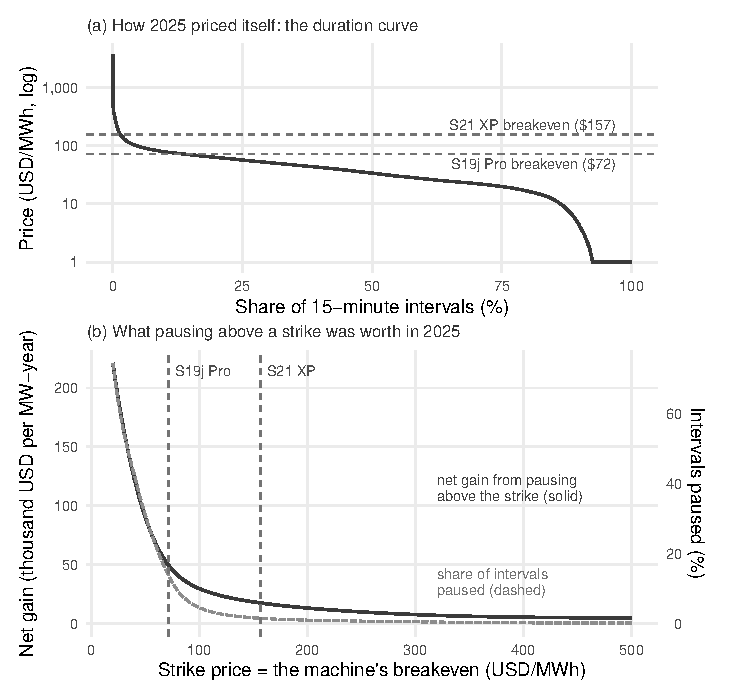
\includegraphics[width=\textwidth]{images/strike_sweep}
  \caption{
    What pausing was worth at LZ\_WEST in 2025, on 15-minute settlement prices. (a)~The price duration curve, with the Chapter~4 breakevens marked; prices below \$1 are drawn at \$1 on the log scale. (b)~The strike sweep: for a 1~MW always-on load that pauses whenever the price exceeds a strike, the annual net gain (solid, left axis) and the share of intervals paused (dashed, right axis), as a function of the strike. % fig-src: analysis/figures/fig_ch6_strike.R on analysis/data/ercot_rtm15_spp_loadzones_2021on.csv.gz (ERCOT MIS 13061)
  }
  \label{fig:strike-sweep}
\end{figure}

Panel~(b) prices the option directly. For every possible strike, it sums what a one-megawatt load would have saved by pausing whenever the price exceeded that strike, over the whole of 2025. Read off the two breakevens: pausing above \$72 earned the S19j~Pro fleet about \$49,000 per megawatt-year, for pausing about 14~percent of intervals, some 1,200 hours. % src: fig_ch6_strike.R console (S19j Pro strike $71.6: $49,116/MW-yr, 13.71%, 1201 h)
Those hours came as 1,018 separate pauses on 297 days: two in five lasted a single quarter-hour and three in five no more than 30 minutes, and the single quarter-hours earned about \$1,000 between them, 2~percent of the total. % src: analysis/checks/ch6_strike_events.R console (LZ_WEST 2025, strike $71.6, runs of consecutive intervals above it: 1,018, median 30 min, mean 1.18 h; 605 of two intervals or fewer = 59.4%; 408 of one interval = 40.1%, worth $1,032 = 2.1% of $49,116; 297 days with a run)
Pausing above \$157 earned the S21~XP fleet about \$17,000 per megawatt-year, for pausing 1.5~percent of intervals, about 130 hours. % src: fig_ch6_strike.R console (S21 XP strike $156.5: $17,280/MW-yr, 1.45%, 127 h)
For scale, running that megawatt around the clock at the index cost about \$370,000 in 2025; the S19j~Pro's option was worth an eighth of the entire power bill. % src: analysis/checks/ch6_contract_pnl.R (RT index $369,454/MW-yr; 49,116/369,454 = 13.3%)

Three readings. First, the money is concentrated: the sweep's steep left side says most of the value lives in the few hundred most expensive hours, which is why Chapter~5 spent so much engineering on catching spikes rather than on shaving averages. % src: ch6_strike_events.R console (the most expensive 200 hours hold 67.3% of the $49,116, the most expensive 400 hours 83.1%)
Nor is it reliably a summer story: in 2025 June to September earned 17~percent of the year, December and January together almost twice as much, and ten days from November to February about a third. On each year's own strike, the same four summer months had carried half the option in 2022 and four-fifths in 2023. % src: ch6_strike_events.R console, seasonality block (2025 at $71.6: Jun-Sep $8,516 = 17.3%; Dec + Jan $15,440 = 1.81 times; the ten best days of Jan, Feb, Nov and Dec $17,154 = 34.9% of the year; own-day strike through ch9_hashprice(), the moving strike of sell_vs_mine.R: Jun-Sep 51.0% of 2022's $131,251 and 79.3% of 2023's $237,653)
Second, the option is worth almost three times as much on the \emph{older} machine. That is Chapter~4's operating leverage arriving on the trading desk: the closer a machine lives to its breakeven, the more often the market crosses it, and the more its off switch earns. The marginal machine holds the fleet's most valuable option. % src: fig_ch6_strike.R console ($49,116 / $17,280 = 2.84)
Third, the sweep is a ceiling: it decides each interval on that interval's own settlement point price, which nobody can read until the interval is over. Decided one settlement interval late instead, with no forecast at all, the \$72 strike kept about \$44,000 in 2025, nine-tenths of the sum; Chapter~9 prices that executable version with each year's own strike. % src: ch6_strike_events.R console (pause when the previous interval's settlement point price exceeds $71.6, booked at each interval's own price, so a late pause into a cheap interval books a loss: $43,750 = 89.1% of $49,116, rows in chronological order through the repeated autumn hour; file order gives $43,749)
A site that must hold every pause and every restart for 30 minutes still keeps about \$42,000, in 869 pauses, and Chapter~5's loop cycles far less than either: it rides the moderate crossings at a lower power target and leaves the pause to a backstop that tripped 0.12 to 0.53 times a day in the backtests (Section~\ref{sec:threerules}). % src: ch6_strike_events.R console, lagged minimum-runtime block (30-minute minimum down and up: $42,358 in 869 pauses = 96.8% of the lagged $43,750); chapter 5 sec:threerules (analysis/ch5-backtest/output/trend_study/multizone_rtm15.csv stops_day: 0.12 to 0.53 pauses per day; LZ_WEST S19j Pro TEST-2025-26 0.53, 284 pauses)

The same settlement data also prices the rest of the contract menu, and Table~\ref{tab:contract-pnl} does so for a flat megawatt in 2025.

\begin{table}[h]
  \centering
  \footnotesize
  \setlength{\tabcolsep}{4pt}
  \begin{tabular}{lrrr}
    \hline
    \textbf{Contract shape} & \textbf{2025 average} & \textbf{Hours/yr} & \textbf{Flat 1 MW} \\
    \hline
    Real-time index (15-min) & \$42.18/MWh & 8,760 & \$369,454 \\
    Day-ahead index (hourly) & \$42.72/MWh & 8,760 & \$374,193 \\
    Fixed \$27.00 (Odessa PPA) & \$27.00/MWh & 8,760 & \$236,520 \\
    Fixed \$43.95 (Corsicana price) & \$43.95/MWh & 8,760 & \$385,002 \\
    \hline
    5x16 window, realized average & \$41.34/MWh & 4,080 & \\
    2x16 window, realized average & \$32.31/MWh & 1,760 & \\
    7x8 window, realized average & \$49.29/MWh & 2,920 & \\
    \hline
  \end{tabular}
  \caption{What a megawatt cost at LZ\_WEST in 2025, by contract shape. Block windows follow the ICE futures definitions \autocite{ice2026ercotnorthpeak,ice2026ercotnorth7x8}; their rows show the realized index average inside each window, a hindsight benchmark rather than a price anyone was quoted in advance. Fixed prices are the two disclosed in SEC filings, applied to every hour of the year; Riot's Corsicana block itself excludes July and August \autocite{cipher10k2024,riot10k2024}. The flexibility option of Section~\ref{sec:strikevalue} comes on top of, and is the same under, every row that permits pausing or sell-back.} % src: analysis/checks/ch6_contract_pnl.R console; fixed prices from cipher10k2024 and riot10k2024; window definitions from ice2026ercotnorthpeak and ice2026ercotnorth7x8
  \label{tab:contract-pnl}
\end{table}

The day-ahead index cost 1.3~percent more than the real-time index. That is what knowing each hour's price a day early happened to cost in 2025, measured after the year closed; nobody quotes it in advance, and it moves from year to year. At LZ\_WEST the day-ahead average ran 2.4, 8.8 and 3.4~percent above the real-time average from 2022 to 2024, and 2.1~percent below it in 2021, the year of Winter Storm Uri; without that February, 2021 would have come out 2.9~percent above as well. Arbitrage keeps the two annual averages within a few percent of each other, even while the two prices in a single hour still differ widely, as Chapter~3 measured. % src: ch6_contract_pnl.R console (LZ_WEST annual DAM minus RT means, MIS 13060 vs 13061: 2021 -2.13%, 2022 +2.37%, 2023 +8.84%, 2024 +3.38%, 2025 +1.28%; 2021 ex Feb +2.87%; 2025 flat 1 MW 374,193 vs 369,454); ch3 quantifies the ~$17 average absolute hourly DART gap
And the block rows are upside down. Everywhere in the textbook world, nights are cheap and weekday daytime is dear; at LZ\_WEST in 2025, the overnight 7x8 window averaged \$49 while the weekday-daytime 5x16 averaged \$41, and the cheapest power of the week was a weekend afternoon at \$32. % src: ch6_contract_pnl.R console (7x8 49.29; 5x16 41.34; 2x16 32.31)
The old off-peak discount did not shrink; it changed sign. Something structural did that, and it is the subject of Sections~\ref{sec:batteries} and~\ref{sec:duck}, because the same force is reshaping what every row of this table will look like next year.

\section{When the Miner Owns the Generator}
\label{sec:ownergen}

Riot and Cipher resell power they contracted for. The step beyond is to own the plant, and on the public record almost no miner in ERCOT has taken it with a plant that sells into the market. MARA bought a Texas wind farm in 2025, 114~MW of turbines with 240~MW of interconnection capacity in Hansford County, for \$49~million; but Hansford County sits in the upper Panhandle, and the federal generator inventory lists the county's one 114~MW wind plant in the Southwest Power Pool's balancing area, not ERCOT's \autocite{mara10k2025,eia860m2026}. % src: mara10k2025 (Note 3: Feb 14, 2025 acquisition, $49.2M, 114 MW nameplate, 240 MW interconnection); eia860m2026 Operating sheet (Plant ID 56905, Great Plains Windpark LLC, Hansford County TX, 114.0 MW onshore wind, Balancing Authority Code SWPP, operating since 2009); consistent with fig_ch3_lz_map.R's "upper Panhandle" gap
Soluna, the most visible behind-the-meter miner, describes its Texas sites as co-located with wind farms belonging to its power partners \autocite{soluna10k2025}. % src: soluna10k2025 (Dorothy "co-located with Briscoe Wind Farm"; Kati "powered entirely by the Las Majadas wind energy project"; Soluna works "with renewable energy developers and power partners")
Riot's 2025 annual report does not mention natural gas generation at all, and Cipher says only that it will evaluate behind-the-meter generation where appropriate \autocite{riot10k2025,cipher10k2025}. % src: riot10k2025; cipher10k2025 ("evaluate opportunities for behind-the-meter generation where appropriate")
ERCOT's rules for selling power also shape the sell-back contracts above.

To sell a megawatt-hour into ERCOT a mine must pass four gates. It registers with the commission before its first day of generation: as a power generation company if it means to sell, whatever its size, or as a self-generator if it means only to serve itself and its plant is a megawatt or more \autocite{puct25109}. % src: puct25109 (16 TAC 25.109(a)(1): PGC registration before the first day of generation, no MW floor; (a)(2): self-generator registration for facilities rated 1 MW or more that are not a PGC)
It enters ERCOT's generator interconnection process, which applies to any unit of a megawatt or more and to any Settlement Only Generator, of any size, a class the fourth gate explains. It pays an interconnection request fee of \$14,000 for a new generator of ten megawatts and up, \$8,000 below that or \$2,300 for a settlement-only unit on the distribution system, and a \$3,000 fee for the full interconnection study \autocite{ercotplanningguide2026,ercotfeeschedule2025}. % src: ercotplanningguide2026 sec. 5.2.1; ercotfeeschedule2025 (interconnection request fees $14,000 / $8,000 / $2,300 SODG; FIS application $3,000)
The fees are the cheap part of that gate. Under the commission's rule the wires utility pays for the transmission upgrades a plant at transmission voltage needs; the plant pays for its own step-up transformers and protection and, under agreements signed after 2025, for interconnection facilities beyond an allowance of \$14~million at 138~kV or less and \$20~million above, in 2024 dollars \autocite{puct25195}. % src: puct25195 (16 TAC 25.195, effective March 7, 2024, Project No. 55566, read 2026-09-27: (b)(1) transmission-level generator, interconnected at or above 60 kV; (f)(1) generator pays "step-up transformers and protective devices at the point of interconnection"; (f)(2), SGIA executed on or before December 31, 2025: TSP pays any new transmission facilities; (f)(3), SGIA executed after December 31, 2025: generator pays interconnection-facility costs above the allowance, TSP pays "any transmission system upgrades"; (f)(3)(A)(i) allowance from January 1, 2026 based on the 2024 amounts of $14,000,000 (138 kV or less) and $20,000,000 (above), adjusted each year by CPI under (A)(ii); (f)(3)(C) above-allowance costs directly billed, collectable as CIAC before construction; (e)(1) a deposit or other security may be required, returned under (e)(1)(A) once service begins)
It registers with ERCOT, for \$500, as a resource entity, the market's name for whoever owns or controls a generator, a battery or a load resource, and it must designate a Qualified Scheduling Entity, the intermediary Chapter~7 describes: a firm it hires or, once it qualifies as one, itself \autocite{ercotfeeschedule2025,ercot2026protocols}. % src: ercotfeeschedule2025 (Resource Entity registration $500); ercot2026protocols sec. 2 (Resource Entity: "An Entity that owns or controls a Generation Resource, an Energy Storage Resource (ESR), a Settlement Only Generator (SOG), or a Load Resource and is registered with ERCOT as a Resource Entity"), sec. 16.5.1.1(1) (each Resource Entity applicant "shall designate" a QSE), sec. 16.2.3.2(1) ("a Resource Entity serving as its own QSE"), sec. 16.2.1 (QSE qualification criteria)
The gate that matters is the fourth, the choice of class. A \glossaryterm{settlement-only-generator}{Settlement Only Generator} is paid for what it exports and nothing else: it may not offer energy, may not be committed or dispatched by ERCOT, and may not sell ancillary services \autocite{ercot2026protocols}. % src: ercot2026protocols sec. 2 (Settlement Only Generator definition)
A full generation resource may do all of those things and in exchange takes on continuous telemetry and a standing offer whenever it is online, the plumbing Chapter~7 describes, plus the duty to run when ERCOT commits it for reliability.

What the grid pays is the price at the generator's own node. A full resource and a Settlement Only Generator normally collect the time-weighted average of the five-minute prices at their bus over the settlement interval, with a floor of minus \$251 per megawatt-hour. The exception is the settlement-only class ERCOT keeps for Private Use Networks, the Settlement Only Transmission Self-Generator, a plant registered with the commission as a self-generator at the first gate. ERCOT settles such a network's net export at the load zone price, which spares it the gap between its node and the zone that West Texas plants live with, in a year when 91~percent of ERCOT's congestion cost arose inside zones rather than between them \autocite{ercot2026protocols,potomac2026somercot}. % src: ercot2026protocols secs. 6.6.1.1 (Resource Node price: time-weighted five-minute LMPs plus the reliability deployment adder, floored at -$251/MWh), 6.6.3.8(1)-(2) (SODG and SOTG paid at their bus, save units that opted out under (5), closed to units not operating or contracted by January 1, 2019, and, under (1)(b), sites where storage is more than half the SOG nameplate), sec. 2 (SOG "comprised of" SODG, SOTG and SOTSG; SOTSG: "connected to the ERCOT transmission system with a rating of one MW or more and is registered with the Public Utility Commission of Texas (PUCT) as a self-generator", registered with ERCOT and modeled under 3.10.7.3), 3.10.7.3(1)(c) ("Energy delivered to ERCOT from an SOTSG shall be settled in accordance with Section 6.6.3.2 ... at a Load Zone"), 6.6.3.2(1)(h) (SOTSG generation in the Load Zone imbalance); the word "self-generator" is kept for the commission's registration class of the first gate and for the name of the ERCOT class that requires it; potomac2026somercot p. 72 (91% intrazonal in 2025)
Generation pays no ERCOT fee on its output; the administration fee falls on metered load only \autocite{ercot2026protocols}. % src: ercot2026protocols sec. 9.16.1 (System Administration Fee on Adjusted Metered Load)
And the captured prices of Section~\ref{sec:btm}, \$19 for wind and \$21 for solar, are what ERCOT's wind and solar plants actually collected on average in 2025: less than half the zone price a load pays. % src: potomac2026somercot p. 20

An owner faces one choice every interval: burn the megawatt-hour into hashes, or sell it. Mining earns the machine's value of the energy, the strike of Section~\ref{sec:arbitrage}; selling earns the node price. For a plant that runs whatever the price, as a wind farm does, any fuel is spent either way and drops out of the choice; a gas plant has a third choice, to stay off, and its rule is a different one. So the owner mines while the price is below the strike and sells when it rises above, which is the same threshold as the buyer who pauses. A buyer pausing above the strike avoids a loss; an owner selling above the strike captures a gain; the sum of price over strike, taken over the hours when it is positive, is identical. For such a network, whose net export is settled at the zone price, the option to sell is therefore worth exactly what panel~(b) of Figure~\ref{fig:strike-sweep} said the option to pause was worth in hindsight: about \$49,000 per megawatt-year for an S19j~Pro fleet in 2025 and \$17,000 for an S21~XP fleet. A plant paid at its own node runs the same rule against that node's price; the captured prices above say how much lower that price runs on average, and whether the gap closes in the scarcity hours is a question about the plant's own bus that this book does not price. % src: fig_ch6_strike.R console ($49,116 and $17,280 per MW-yr); analysis/checks/sell_vs_mine.R (identity: sum of max(P - V, 0) is the same sum whether the MWh was avoided or sold)
The option looks small only because an owner measures it against the whole revenue of the machines, about \$630,000 per megawatt-year for the S19j~Pro, while a spot buyer measures the same dollars against a margin of about \$260,000, the machines' revenue less the power bill. % src: sell_vs_mine.R console, "2025 denominators" block: revenue $628,351 (mean moving strike $71.7 over all 8,760 h of 2025), power bill $369,454, margin $258,897

And it pays out like insurance. Run the same rule with each year's own hashprice, so that the strike moves as the machines' economics moved: the S19j~Pro's strike stood near \$440 in 2021 and the option still paid about \$960,000 per megawatt-year to a plant that kept running through the February storm, 94~percent of it in that one week; in 2023 it paid about \$240,000; in 2025 about \$51,000, a shade above the fixed-strike figure because the strike drifted with hashprice through the year \autocite{ercotrtmhist}. % src: analysis/checks/sell_vs_mine.R console, moving-strike table (2021 $957,665, of which Feb 14-20 $895,877 = 94%; 2023 $237,653; 2025 $51,499 per MW-yr; strikes $438 / $104 / $72); real-time settlement prices from ERCOT MIS report 13061
Once the gates are passed it costs nothing more to hold and pays little in a calm year; in 2021, a scarcity year, it paid, almost entirely in one week, about a quarter of what the machines earned all year, at a \$9,000 cap that today's rules no longer allow (Section~\ref{sec:ordc}). % src: sell_vs_mine.R console, "2021 denominators" block (sell option $957,665 against revenue at the moving strike, about 25%); the $9,000 cap of 2021: chapter 3 sec:ordc (ercot2021hcapnotice, HCAP $9,000 until January 1, 2022; potomac2021som p. vi, "the VOLL and HCAP of $9,000"); today's rules: chapter 3 sec:ordc (puct25509 (b)(6)(B) HCAP $5,000 and (c) the Emergency Pricing Program)
That week is also where the identity with the buyer breaks: a buyer who paused kept those dollars whatever happened upstream, while an owner kept them only on the megawatt-hours its plant delivered, in a week when about half of ERCOT's generation was offline \autocite{ERCOTUpdate2021}. % src: ch2 sec. on Uri (ERCOT Apr 27, 2021 update: 52,037 MW unavailable at the worst point, Feb 16)
The one place the owner does better than a plant that must sell is the roughly 490 hours of 2025 in which West Texas prices went negative: selling those hours cost money, and mining them did not. % src: sell_vs_mine.R console, "2025 denominators" block (count of negative-price 15-minute intervals in LZ_WEST / 4)

Few miners own generation because the prize of owning was never the electrons. At the captured prices above, a wind farm's energy is worth less to its owner than a mine would pay for it, so the generator would rather sell across the fence to a mine than into the grid, and the mine collects most of the discount by contract without buying a single turbine. The scarce thing is the plant's interconnection, in a market where requests in the large-load queue Chapter~3 described run to several times the system's peak, and a miner gets it by sitting behind the plant's meter, not by owning the plant. That is what the behind-the-meter arrangements of Section~\ref{sec:btm} are really buying.

\section{The Competition Arrived: Batteries}
\label{sec:batteries}

The strike sweep of Figure~\ref{fig:strike-sweep} pays out of price extremes: the option earns when prices spike, and to a lesser degree the bill shrinks when prices go negative. A miner holding that option should therefore watch, with professional interest, the one asset class whose entire business is deleting price extremes: grid batteries, which ERCOT calls \glossaryterm{energy-storage-resource}{energy storage resources} (ESRs). A battery buys the trough and sells the peak; every megawatt of it lifts the floor and shaves the spike that the miner's option was written on.

They arrived fast. Counting operating units by their in-service dates, ERCOT's battery fleet grew from about 4.4~GW of nameplate capacity at the start of 2024 to 8.5~GW a year later, 14.2~GW by the start of 2026, and 18.1~GW by mid-2026 \autocite{eia860m2026jul}. % src: fig_ch6_batteries.R console on analysis/data/ercot_capacity_additions_2026-07.csv (EIA-860M July 2026)
The market monitor's own ledger runs higher still, over 17~GW and 31,500~MWh by the end of 2025, up almost 80~percent in a year, with average duration stretching from 1.67 to 1.83 hours; the two counts differ in what they include and when, but they agree on the slope \autocite{potomac2026somercot}. % src: potomac2026somercot, pp. ii, 21-22 (IMM end-2025 >17 GW vs EIA-860M in-service 14.2 GW at 2026-01: different counting bases, both quoted as their own)
On a summer evening in 2025 the fleet was supplying an average of 4~GW in the eight-p.m.\ hour, filling the gap that solar leaves as it sets \autocite{eia2025ercotmix}. % src: eia2025ercotmix

\begin{figure}[htbp]
  \centering
  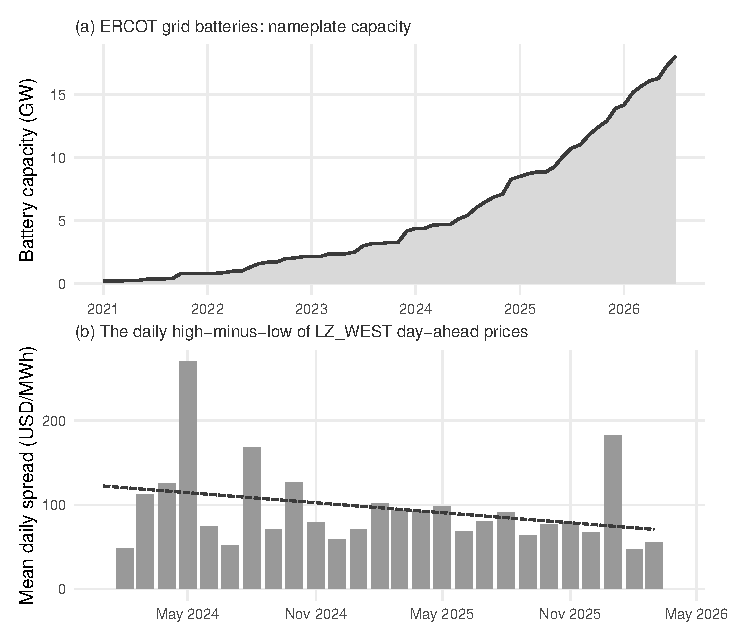
\includegraphics[width=\textwidth]{images/batteries_spreads}
  \caption{
    (a)~ERCOT grid batteries: cumulative nameplate capacity by operating date, from the federal generator inventory (EIA-860M, July 2026). (b)~The raw material of storage arbitrage: the monthly mean of each day's spread between the highest and lowest hourly day-ahead price at LZ\_WEST, with a linear trend. As the fleet roughly tripled, the average daily spread compressed from \$112 in 2024 to \$82 in 2025. % fig-src: analysis/figures/fig_ch6_batteries.R; console: spread 2024 $112.4, 2025 $82.0; capacity from analysis/data/ercot_capacity_additions_2026-07.csv
  }
  \label{fig:batteries-spreads}
\end{figure}

The price effects are no longer conjecture; the market monitor states them outright. Price spikes in summer 2025 were 40~percent less frequent than in summer 2024, because the added storage absorbed the system's ramps \autocite{potomac2026somercot}. % src: potomac2026somercot, p. iii
The ancillary service markets, where batteries found their first profits, saturated even faster: the average price of ECRS collapsed from about \$77 per megawatt per hour of standby in 2023 to under \$10 in 2024, a drop the market monitor puts down to new supply, batteries above all \autocite{potomac2024som}. % src: potomac2024som pp. ii, vi (ECRS $76.77 -> $9.62; "This drop was caused by an increase in supply, particularly from energy storage resources (ESRs)"), as chapter 7 prints it; until 2026-09-26 this line added an unlabelled "part correction" inference from potomac2026somercot, cut to match chapter 7 (PER-3 review round)
By 2025 batteries dominated ancillary supply so thoroughly that their own ancillary revenue fell by more than a third even as their fleet grew \autocite{potomac2026somercot}. % src: potomac2026somercot, p. 23 (AS revenue fell >37%)
Figure~\ref{fig:batteries-spreads}(b) shows the version of this squeeze that a miner feels: the average daily high-minus-low spread at LZ\_WEST, the raw material of storage arbitrage and strike alike, compressed by more than a quarter from 2024 to 2025. One year's correlation is not proof of cause, but the direction matches what the monitor attributes to storage, and the mechanism is not subtle.

So are batteries simply eating the miner's lunch? Partly: every dollar in Figure~\ref{fig:strike-sweep}(b) is smaller than it would have been in 2023's wilder market. But two structural differences keep the trades distinct. A battery is duration-limited: at 1.8 hours of storage it must choose which spike to sell into, so its arbitrage saturates against its own fleet, which is exactly what the ancillary collapse shows. % src: potomac2026somercot, pp. 21-22 (average ESR duration 1.83 h at end-2025, as chapter-6.tex:234)
It also pays for every round trip: it gives back about 85~percent of the energy it takes in, so it buys about 1.2 megawatt-hours for every one it sells, and each cycle wears its cells a little \autocite{potomac2026somercot,nlr2025atbbattery}. % src: potomac2026somercot, p. 21 (ESR fundamentals: a net load, losses occur throughout the cycle, NREL 2024 ATB round-trip efficiency 85%); 1 / 0.85 = 1.18 MWh bought per MWh sold; nlr2025atbbattery (2025 ATB: roundtrip efficiency 85%; about one cycle per day, and degradation is a function of the usage rate of the model; fixed O&M carries augmentation to hold rated capacity over a 15-year life)
A pausing miner has no state of charge and owes no energy back: it can stay off for an hour or a week if the price demands it, and when it is not pausing it is not idle capital waiting for volatility; it is mining. The battery needs the spread to justify existing. The miner's option is a bonus written on top of a business that pays for itself at \emph{average} prices, so when the spreads get thin, the battery feels it first.

\section{Renewables and the Shape of the Day}
\label{sec:duck}

The second structural force is the reason the spreads existed in the first place. Wind and solar together supplied 34.6~percent of ERCOT's energy in 2024 and 37.5~percent in 2025, with all of the growth coming from solar, whose share jumped from 10.4 to 13.9~percent \autocite{ercot2025factsheet,ercot2026factsheet}. % src: ercot2025factsheet (2024: wind 24.2 + solar 10.4); ercot2026factsheet (2025: wind 23.6 + solar 13.9); potomac2026somercot confirms 10.4 -> 13.9
Solar output grew 49~percent in 2025 alone, and summer midday solar production doubled between 2023 and 2025, from about 12 to about 24~GW at noon \autocite{potomac2026somercot,eia2025ercotmix}. % src: potomac2026somercot (solar +49%, 6% curtailed); eia2025ercotmix (12 -> 24 GW summer noon)
Wind and solar bid into the market at their marginal cost, which is approximately zero, and when they cover enough of demand they set the price at their level: the market monitor counts hundreds of hours per year with prices at or below zero \autocite{potomac2026somercot}. % src: potomac2026somercot (zero-marginal-cost growth; hundreds of hours at or below $0/MWh)

\begin{figure}[htbp]
  \centering
  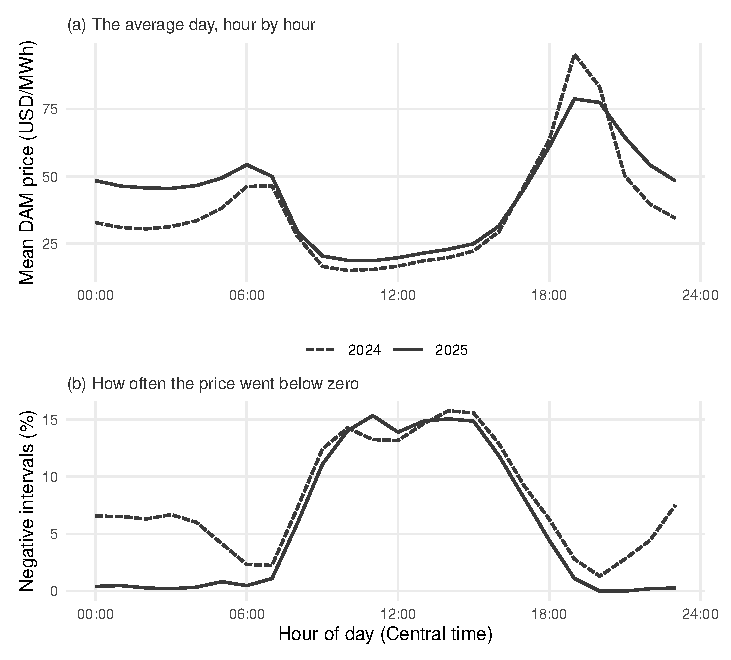
\includegraphics[width=\textwidth]{images/duck_lzwest}
  \caption{
    The duck at LZ\_WEST. (a)~Average day-ahead price by hour of day, by year: the midday trough deepens as solar grows, while the evening ramp holds its height. (b)~The share of 15-minute real-time settlement intervals with negative prices, by hour: overnight negatives, a wind signature, nearly vanished in 2025 as batteries and demand growth absorbed them; midday negatives, the solar signature, persist. % fig-src: analysis/figures/fig_ch6_duck.R; panel (a) on analysis/data/ercot_dam_spp_loadzones_2021on.csv.gz (ERCOT MIS 13060), panel (b) on analysis/data/ercot_rtm15_spp_loadzones_2021on.csv.gz (ERCOT MIS 13061)
  }
  \label{fig:duck}
\end{figure}

Plot the average price against the hour of the day and the result is the grid world's most famous silhouette, the \glossaryterm{duck-curve}{duck curve}: a deep belly at midday where solar floods the market and a steep neck in the evening when it withdraws. Figure~\ref{fig:duck} draws LZ\_WEST's duck. In 2025, midday hours averaged about \$21 while the evening ramp averaged about \$72: more than three times as much, a few hours apart on the same average day. % src: fig_ch6_duck.R console (2025: midday 11-15h DAM mean $20.8, evening 18-21h mean $72.4; the 2024 values are $17.7/$80.7)
Negative prices tell the same story with a twist: their overall share fell from 8.1~percent of intervals in 2024 to 5.6~percent in 2025, but the composition flipped, with the old overnight wind-driven negatives nearly disappearing while the midday solar negatives held on. % src: fig_ch6_duck.R console (negative share 8.1% 2024 -> 5.6% 2025; overnight negatives collapse)
Batteries charging through the cheap hours absorbed the negatives that fit inside their duration; the midday solar surplus still outruns them. The market monitor adds the system-level confirmation: the tightest hours of the ERCOT day have migrated from the traditional four-to-five-p.m.\ demand peak to the seven-to-nine-p.m.\ \glossaryterm{net-load}{net-load} peak, the hour when demand minus renewables is highest, which is the hour solar leaves \autocite{potomac2026somercot}. % src: potomac2026somercot (tightest period shifted from 4-5 p.m. to 7-9 p.m.)

This is what inverted Table~\ref{tab:contract-pnl}'s block rows. The 5x16 weekday-daytime window now contains the solar belly, so its average sags; the 7x8 night window contains no solar at all, so it holds firm; the weekend 2x16 combines the belly with weekend demand and becomes the cheapest shape on the menu. West Texas sharpens everything: the market monitor notes that the West zone managed to post both the highest average price of any zone in 2025 \emph{and} the most negative-price intervals, because the wind-and-solar-rich Panhandle is export-constrained while the demand-heavy Permian is import-constrained \autocite{potomac2026somercot}. % src: potomac2026somercot (West zone: highest average price, most negative intervals, most price spikes)
A flat consumer would call that the worst of both worlds. For a load that follows price, that is the best of both: deeper discounts to mine through and taller spikes to sell absence into, which is why it is this book's home zone.

For the miner, then, the renewable buildout helps on both sides of the ledger. It drags the \emph{average} down, which fattens the mining margin at any hashprice; and it steepens the \emph{shape}, which raises what flexibility earns. The daily price pattern rewards consumption at midday and curtailment during the evening ramp. Machines that pause in seconds suit that daily rhythm, plus the handful of days a year, winter ones included, when the price becomes a crisis. % src: ch6_strike_events.R console (2025: ten days of January, February, November and December hold 34.9% of the S19j Pro's option at $71.6)

\section{The Market Just Changed: RTC+B}
\label{sec:rtcb-firstlook}

Everything measured so far in this chapter was priced under market rules that ended in December 2025. On December~5, ERCOT switched on Real-Time Co-optimization plus Batteries (RTC+B), which it calls the most substantial change to the real-time market since the nodal design launched in 2010 \autocite{ercot2025rtcblive}. % src: ercot2025rtcblive (go-live Dec 5, 2025; "most substantial enhancement... since its inception in 2010")
The change is easy to state in this book's vocabulary: before, ERCOT bought energy every five minutes but reserved ancillary capacity a day ahead; now the real-time engine buys energy \emph{and} every ancillary product together, every five minutes, with battery state of charge modeled explicitly, so a megawatt can flow to whichever use is worth most right now. % src: ercot2025rtcblive (co-optimized energy + AS procurement in real time; battery SOC modeling)
The project was ordered by the Texas commission in 2019, took six years to build, and ERCOT projects the efficiency gain at over a billion dollars of wholesale cost per year \autocite{ercot2025rtcblive}. % src: ercot2025rtcblive (PUCT Project No. 48540, 2019 directive; Collins quote: "projected wholesale market savings exceeding one billion dollars annually")

The early reviews were undramatic, which for a market redesign is praise. Day-ahead ancillary prices spiked on the go-live day itself, then normalized within days; the market monitor put 15 of December's 24 priciest day-ahead Non-Spin hours on December 5 and attributed them to uncertainty about the change. The real-time market then worked as expected, with no major malfunction but a short stabilization list, until Winter Storm Fern gave it a real test in late January. Batteries repriced their day-ahead ancillary offers upward in every product, and the reason is structural: the redesign lets a resource sell reserves straight into real time, which makes a day-ahead position riskier for anything duration-limited \autocite{potomac2026somercot,ercotcmu2026feb}. % src: potomac2026somercot p. 40 (15 of 24 highest-priced December DAM Non-Spin hours on Dec 5, 2025; "AS prices normalized again a few days after RTC go-live"), Appendix I pp. A-2 to A-5 ("operating largely as expected without major dysfunctions"; Figure A2, ESR day-ahead AS offers repriced upward in all five products; p. A-3 gives the duration-constraint and sell-into-real-time reason and says the monitor predicted it); ercotcmu2026feb slides 1-2 and the RTC+B Stabilization Activities slide

\begin{figure}[p]
  \centering
  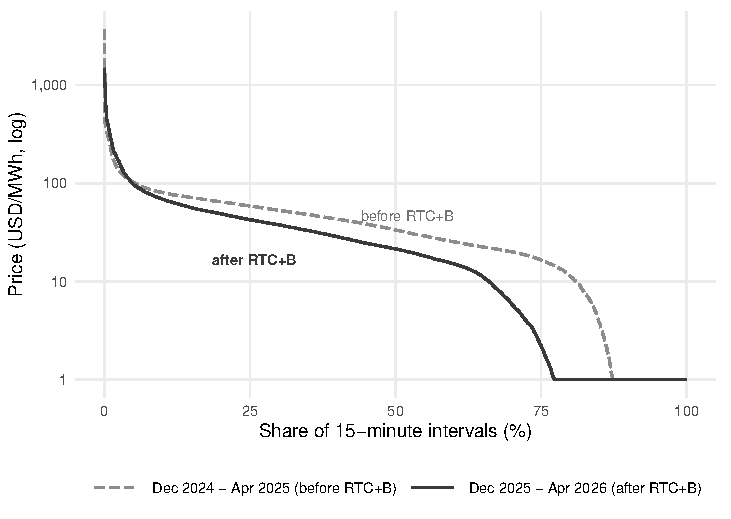
\includegraphics[width=\textwidth]{images/rtcb_volatility}
  \caption{
    A season-matched first look at prices under RTC+B: LZ\_WEST 15-minute settlement prices for December~5 to April~20, the winter before go-live against the first winter after. Duration curves on a log scale; prices below \$1 are drawn at \$1. The average fell, negative-price intervals doubled, the moderate tail thickened, and the extreme tail shortened. % fig-src: analysis/figures/fig_ch6_rtcb.R on analysis/data/ercot_rtm15_spp_loadzones_2021on.csv.gz (ERCOT MIS 13061)
  }
  \label{fig:rtcb}
\end{figure}

Figure~\ref{fig:rtcb} makes the comparison this book can make honestly: the same calendar window, December~5 through April~20, in the last winter of the old rules and the first winter of the new ones, at LZ\_WEST on settlement prices. The average fell from about \$42 to \$34/MWh. % src: fig_ch6_rtcb.R console (season-matched mean $42.56 -> $33.60)
Negative-price intervals doubled, from 9.5 to 18.8~percent of the window. % src: fig_ch6_rtcb.R console (negative share 9.54% -> 18.76%)
The extreme tail shortened, with the window's maximum falling from about \$3,700 to \$1,500, while the moderate tail thickened: the 99th-percentile price rose from about \$230 to \$300. % src: fig_ch6_rtcb.R console (max $3,686.94 -> $1,485; P99 $228 -> $295)

Every caveat belongs in the same breath as the numbers. This is one winter against one winter; each window contains one winter storm (Winter Storm Kingston before, Fern after); the battery fleet grew almost 80~percent and solar kept building through the comparison, so this figure measures RTC+B \emph{plus} everything else that changed; and the market monitor's first full assessment will not arrive until its next annual report \autocite{potomac2026somercot}. % src: potomac2026somercot (ESR +80% in 2025); fig_ch6_rtcb.R window definition (Kingston Feb 2025 in the before-window, Fern Jan 2026 after); labeled first look, not attribution
Call it a first look. But notice what each shift in it means for a flexible load: a cheaper average megawatt-hour, twice as many intervals that pay you to consume, and more frequent moderate spikes for the strike to harvest. Against that, it has fewer of the catastrophic prices in which, as Section~\ref{sec:strikevalue} showed, most of the option's value has lived. If the pattern holds, the new market pays flexibility more often and in smaller amounts, and a machine that earns its option in small bites, over and over, is built for that world.

\bigskip

The chapter's ledger, then. The contract sets your average cost and decides whether your off switch is connected to the market; the machine sets the strike; and in 2025 at LZ\_WEST the strike was worth about \$49,000 per megawatt-year on the marginal fleet in hindsight and \$44,000 decided one interval late, about an eighth of the power bill, before a single new market product enters the picture. % src: fig_ch6_strike.R console ($49,116); ch6_strike_events.R console (lagged $43,750); ch6_contract_pnl.R (RT index $369,454/MW-yr: 13.3% and 11.8%)
Batteries, renewables, and RTC+B are reshaping the prices underneath it, compressing the old spreads while multiplying the small ones. But pausing against price is still only the first way ERCOT pays a flexible load, and it is the passive one: the market never knows the miner is there; it just sees demand vanish above a threshold. The second way is louder. ERCOT runs standing markets that pay loads simply to be \emph{ready} to vanish on command, whether or not the command ever comes, and RTC+B just rebuilt those markets from the ground up. These are the ancillary service markets of Chapter~7.

\chapter{Ancillary Services: Getting Paid to Stand By}
\chaptermark{Ancillary Services}
\label{ch:ancillary}

Everything the book has priced so far is a reaction: the machine watches the price and steps aside when electricity costs more than it earns. Chapter~3 gave a first look at a second set of markets where the product is not energy but readiness. In the ancillary service markets, ERCOT pays resources by the hour simply to stand ready to act, whether or not the call ever comes, and a machine whose whole talent is stepping aside in seconds would seem to be the perfect seller. For one week in 2021, ancillary services were the most lucrative market a megawatt could enter. What happened since is a lesson in how fast open markets eat a good trade, and why the off switch's second income stream is now a complement to the strike price of Chapter~6 rather than a substitute for it.

One unit warning before the tour. Ancillary prices are \glossaryterm{capacity-price}{capacity prices}: dollars per megawatt for each hour of standby, written \$/MW per hour, not dollars per megawatt-hour of energy. A resource earns the clearing price on its committed megawatts every hour it holds the award, on top of whatever it does or does not earn selling or consuming energy. Keep the capacity-price unit separate from the energy-price unit. % src: MCPC definition; the internal AS workbook's own $/MWh axis mislabel is the cautionary case (not cited)

\section{What ERCOT Buys}

ERCOT procures five ancillary services, each a different flavor of readiness, distinguished by how fast it must act and how long it must last \autocite{ercot2026protocols}. % src: ercot2026protocols sec. 2 definitions; tab:as-products
Table~\ref{tab:as-products} lists them with the response clock that defines each one.

\begin{table}[htbp]
  \centering
  \footnotesize
  \setlength{\tabcolsep}{4pt}
  \begin{tabular}{lllr}
    \hline
    \textbf{Service} & \textbf{Acts within} & \textbf{Sustains} & \textbf{2025 avg MW} \\
    \hline
    Reg-Up & 5 s & 30 min & 436 \\
    Reg-Down & 5 s & 30 min & 402 \\
    RRS & 0.25--0.5 s & 15 min to 1 h & 2,739 \\
    ECRS & 10 min & 1 h & 1,416 \\
    Non-Spin & 30 min & 4 h & 2,885 \\
    \hline
  \end{tabular}
  \caption{ERCOT's five ancillary services. Response and sustain requirements from the Nodal Protocols, with the sustain times in force since RTC+B; average procured quantities are day-weighted means computed from ERCOT's published 2025 AS quantities workbook. RRS is provided in three sub-forms with different clocks (see text) \autocite{ercot2026protocols,ercot2025nprr1282,potomac2026somercot,ercotasmeth2025}.} % src: ercot2026protocols sec. 2 (Reg 5 s; FFR 15 cycles; Non-Spin 30 min; ECRS 10 min); secs. 8.1.1.3.1(2), 8.1.1.3.2(4), 8.1.1.3.3(2), 8.1.1.3.4(2) (sustain: Reg 30 min; RRS 30 min if SCED-dispatchable, one hour otherwise, 15 min for FFR from a load; Non-Spin four consecutive hours; ECRS one hour); ercot2025nprr1282 (effective 2025-12-05: Reg and SCED-dispatchable RRS 15 to 30 min, ECRS two consecutive hours to one; sec. 2 and sec. 3.17.4(1) still print ECRS as two consecutive hours); RRS 0.5 s is the load relay's clock (ercotnog2026 sec. 2.3.1.2, as the text below prints it) and governors begin in about 3.5 s (FERCNERCFeb2021 appendix p. 19, chapter 2 sec:inertia); potomac2026somercot p. 38 (LFC signals every 4 s); ercotasmeth2025 workbook (436/402/2,739/1,416/2,885 MW day-weighted means)
  \label{tab:as-products}
\end{table}

Regulation is the fine motor control. ERCOT's Load Frequency Control sends a correction signal every four seconds, and regulation resources must follow it within five, nudging output or consumption up (Reg-Up) or down (Reg-Down) to hold the grid at 60~Hz between economic dispatch runs \autocite{potomac2026somercot,ercot2026protocols}. % src: potomac2026somercot p. 38 (LFC every 4 s); ercot2026protocols sec. 2 (respond within five seconds)

Responsive Reserve is the crash barrier: capacity that arrests a falling frequency in the first seconds after a big generator trips \autocite{ercot2026protocols}. % src: ercot2026protocols sec. 2 RRS definition ("arrest frequency decay within the first few seconds")
It comes in three sub-forms. The first is the primary frequency response of Section~\ref{sec:inertia}, which every generator must be able to provide: its turbine governors begin about three and a half seconds after a trip and feed in more steam or gas as frequency falls, without waiting for any instruction. Storage and controllable load resources provide it too \autocite{FERCNERCFeb2021,potomac2026somercot}. Batteries provide nearly all of the \glossaryterm{fast-frequency-response}{fast frequency response} (FFR), full output within a quarter second of a frequency trigger, sustained at least fifteen minutes, but any load fast enough may qualify for it too \autocite{ercot2026protocols,potomac2026somercot}. % src: FERCNERCFeb2021 appendix E, appendix p. 19 ("conventional generators typically begin their governor response in about 3.5 seconds"), as chapter 2 sec:inertia prints it; ercot2026protocols sec. 2 FFR definition ("provision by a Resource"; 15 cycles = 0.25 s; sustain 15 min), sec. 3.17.2(3)(b) (RRS from Resources capable of FFR), sec. 8.1.1.3.2(4) ("non-Controllable Load Resources qualified to provide FFR", 15 min); potomac2026somercot p. 132 (FFR "provided almost exclusively by batteries"; PFR "provided by generators, storage resources, and controllable load resources") and p. 38 (PFR, "which all generators must be able to provide")
And loads provide the bluntest form of all: an \glossaryterm{under-frequency-relay}{under-frequency relay} (UFR), a hardware tripwire that disconnects the whole site within half a second when frequency falls to its setting, with nothing in software between the frequency and the breaker \autocite{ercotnog2026}. % src: ercotnog2026 sec. 2.3.1.2 (total interruption within 30 cycles = 0.5 s incl. relay and breaker); trip setting no lower than 59.70 Hz

ECRS, launched June 10, 2023 as the first new daily procured service in more than twenty years, is the ten-minute reserve: capacity ERCOT can call to restore the crash barrier after it has been used, sustained for at least an hour (two hours until RTC+B cut it in December 2025) \autocite{ercotecrs2023launch,potomac2023som,ercot2025nprr1282}. % src: ercotecrs2023launch ("first daily procured Ancillary Service introduced to the ERCOT market in more than 20 years"); potomac2023som p. 96 (go-live June 10, 2023); ercot2026protocols sec. 2 (10 min), secs. 8.1.1.2.1.7(3), 8.1.1.3.4(2) (maintain the award at least one hour; sec. 2 and sec. 3.17.4(1) still print two consecutive hours); ercot2025nprr1282 (two consecutive hours to one hour, eff. Dec 5, 2025)
Non-Spin is the slow reserve: thirty minutes to arrive, four hours of endurance, the service that covers a forecast bust rather than an instant failure \autocite{ercot2026protocols}. % src: ercot2026protocols sec. 2 Non-Spin definition (30 min, four consecutive hours)

Two facts about this shopping list matter for everything that follows. First, it is large: about 7,900~MW of standby held every average hour of 2025, and the market monitor complains, year after year, that ERCOT buys roughly twice the reserves a reasonable reliability standard would require \autocite{ercotasmeth2025,potomac2026somercot}. % src: ercotasmeth2025 workbook (sum of the five day-weighted means = 7,878 MW); potomac2026somercot pp. 3, 39 ("more than double")
Second, loads are welcome nearly everywhere in it. Every service except Regulation can be provided by a load with nothing more sophisticated than an on-off switch, and every service on the list, Regulation included, can be provided by a load that qualifies as controllable \autocite{ercot2026protocols}. % src: ercot2026protocols sec. 3.6.1 (Load Resource participation by service); sec. 3.16 caps
ERCOT pays the same clearing price whether readiness comes from a turbine that can spin up or a mining hall that can go quiet.

A sixth service is on its way. The Dispatchable Reliability Reserve Service, a slower reserve that must reach its level within two hours and hold it for four, was approved in July 2026 but waits on system changes that ERCOT's project list targets for late 2028; only generators may sell it, and its arrival cuts Non-Spin's endurance to two hours \autocite{ercot2026nprr1309,ercot2026rrprojects}. % src: ercot2026nprr1309 (PUCT approved July 9, 2026, effective upon system implementation; its gray boxes in ercot2026protocols Aug 1, 2026: sec. 2 DRRS definition; new sec. 3.17.5, capacity from Off-Line or On-Line Generation Resources that ramp within two hours and run at least four consecutive hours; sec. 2 Non-Spin definition, sec. 3.17.3(1)(a)(ii),(b)(ii) and sec. 8.1.1.3.3(2), four consecutive hours to two; PUCT Report 1309NPRR-35, whose justification says the NPRR was developed pursuant to PURA 39.159(d), statute not read); ercot2026rrprojects (project 575-01 NPRR1309, status Initiation, target end November 30, 2028)

\section{What Standing By Paid, 2021 to 2026}

Figure~\ref{fig:as-history} shows the five clearing-price histories on one log scale, and Figure~\ref{fig:as-standing-revenue} compresses each year into a single number: the \glossaryterm{standing-revenue}{standing revenue}, what one megawatt earned by holding the award through every hour of the year, before any energy consequences. It is a ceiling, not a forecast: it assumes an award in every hour at the day-ahead clearing price, with no QSE fee, no deployment cost and no failed-performance event.

\begin{figure}[htbp]
  \centering
  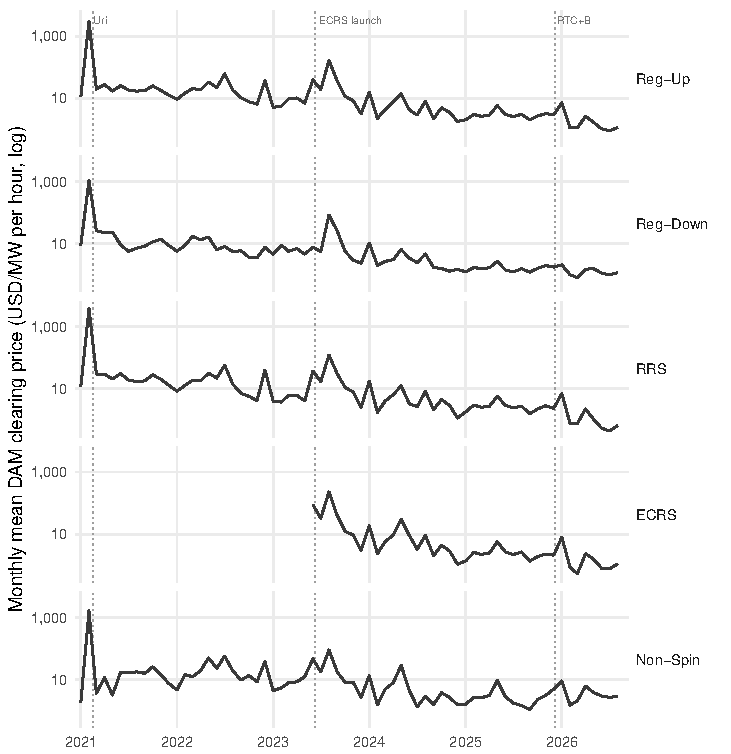
\includegraphics[width=\textwidth]{images/as_price_history}
  \caption{
    Monthly mean day-ahead clearing prices for the five ancillary services, 2021 to mid-2026, log scale. The February 2021 spike is Winter Storm Uri; ECRS appears at its June 2023 launch and spends its first year as the most expensive product on the board; everything decays toward single digits as batteries flood in; RTC+B changes the market's plumbing in December 2025. Prices below \$0.10 are drawn at \$0.10. % fig-src: analysis/figures/fig_ch7_as_history.R on analysis/data/ercot_dam_as_mcpc.csv.gz
  }
  \label{fig:as-history}
\end{figure}

Act one is Uri. During the February 2021 emergency, day-ahead ancillary prices cleared above \$25,000 per megawatt for single hours, nearly three times the era's \$9,000 system-wide offer cap, because the clearing algorithm priced the opportunity cost of scarce capacity without any cap of its own \autocite{potomac2021som}. % src: potomac2021som p. vi ("MCPCs ... in excess of $25,000 per MW"; DAM algorithm opportunity-cost design)
The market monitor called the outcome a roughly \$2~billion overvaluation of ancillary services, and the rules were changed within months: ancillary prices are now capped at the system-wide offer cap, and the cap itself was cut to \$5,000 the following January \autocite{potomac2021som}. % src: potomac2021som p. vi ($2B overvaluation; NPRR1080 June 2021; HCAP to $5,000 effective Jan 1, 2022)
For sellers, that one storm made the year. A megawatt that held RRS through all of 2021 collected about \$2.7~million, and 91~percent of it accrued in Uri week alone. % src: fig_ch7_as_history.R console (RRS 2021 total $2,735,205; Uri week Feb 14-20 $2,485,794 = 91%)

Act two is the ECRS misadventure. The new ten-minute product launched in June 2023 into a hot summer, and ERCOT held it back so firmly during tight hours that the market behaved as if the system were short when it was not. The market monitor concluded that the way ECRS was procured and withheld created artificial shortage pricing that roughly doubled real-time energy prices from June through December and added more than \$12~billion of real-time market costs \autocite{potomac2023som}. The service itself cost more than \$600~million to procure and bought a computed reliability benefit of about \$12~million, a fifty-to-one ratio of cost to value. % src: potomac2023som pp. ii, ix, 11 (doubled RT prices Jun-Dec; >$12B excess; $600M procurement vs $12M value = 50x)
The market monitor put ECRS's 2023 average near \$77 per megawatt per hour of standby, over triple the RRS average, and a megawatt standing in the product from launch day collected \$286,000 in seven months \autocite{potomac2023som}. % src: potomac2023som p. ii ($76.77, over triple RRS; the IMM average is not the simple hourly mean, which is $58.15 per fig_ch7_as_history.R console); fig_ch7_standing_revenue.R console (ECRS 2023 partial-year $286,136)


Act three is the flood, and Chapter~6 already introduced its protagonist. Batteries are nearly ideal ancillary machines, and as their fleet quadrupled they moved into these markets first: the monitor's phrasing is simply that storage \emph{flooded} the ancillary markets and prices fell \autocite{potomac2026somercot}. % src: potomac2026somercot p. 22 ("As ESRs have flooded the AS markets, AS prices have fallen"); quadrupled = 4.4 -> 18.1 GW per ch6 fig_ch6_batteries.R (EIA-860M July 2026)
ECRS collapsed from about \$77 to under \$10 per megawatt per hour in a single year, a drop the market monitor puts down to new supply, batteries above all \autocite{potomac2024som}. % src: potomac2024som pp. ii, vi ($76.77 -> $9.62; "This drop was caused by an increase in supply, particularly from energy storage resources (ESRs)")
ERCOT's own attempt at a repair, formal triggers for releasing the reserve to the market, was rejected by the commission in July 2024; ERCOT applied the triggers anyway, without the rule's \$750/MWh floor on the reserve's energy offers, and the monitor judged the method flawed, since it let artificial shortages set in before the reserve was released \autocite{ercotnprr1224,potomac2024som}. % src: ercotnprr1224 (posted March 27, 2024, urgent; manual ECRS release when the power balance violation is at least 40 MW for ten consecutive minutes; ECRS Energy Offer Curves floored at $750/MWh; Board recommended June 18, 2024; PUCT rejected July 25, 2024); potomac2024som pp. xxi, 13 (PUCT rejection July 2024, then "ERCOT still implemented the deployment process proposed by NPRR 1224, but without the $750 per MWh energy offer floor"; "effectively forcing the real-time market into artificial shortage conditions before releasing ECRS"), p. 14 (3 of 24 costly 2024 events had NPRR 1224 deployments)
In 2025 every product fell again, and the total cost of all five services dropped to 39 cents per megawatt-hour of load served, the lowest since 2020, down from \$29.59 in Uri's year \autocite{potomac2026somercot,potomac2021som}. % src: potomac2026somercot p. 3 ($0.39/MWh load, -60%, lowest since 2020); potomac2021som p. 43 ($29.59 in 2021)

\begin{figure}[htbp]
  \centering
  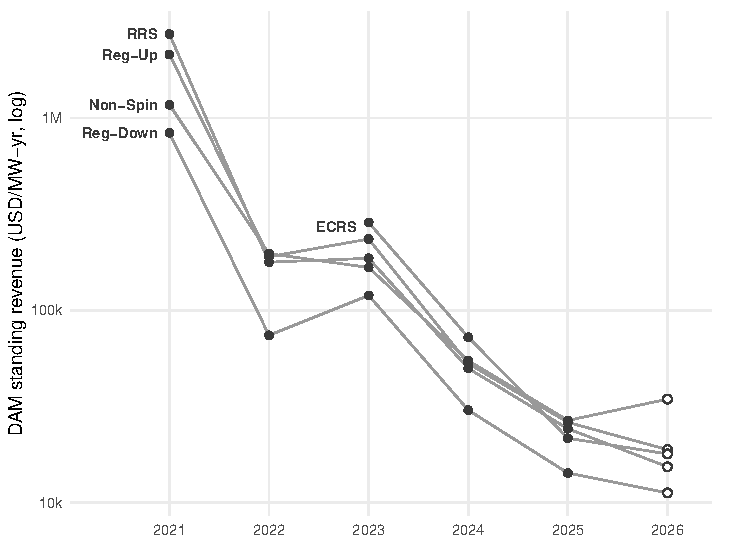
\includegraphics[width=\textwidth]{images/as_standing_revenue}
  \caption{
    Standing revenue by product and year: what one megawatt earned by holding each award through every hour, log scale. RRS fell from \$2.74~million per megawatt-year in 2021 to \$24,000 in 2025, a 113-fold decline; the whole product stack, four products in 2021 and five by 2025, fell 61-fold. The 2026 run rate is lower again for every product except Non-Spin, the only one rising. ECRS's 2023 is a partial year from its June launch; the 2026 open markers are the total to date, annualized. % fig-src: analysis/figures/fig_ch7_standing_revenue.R; console: RRS 2,735,205 -> 24,168; stack 6,886,902 -> 112,749
  }
  \label{fig:as-standing-revenue}
\end{figure}

Add the products together, a sum no single megawatt could collect, and the whole product stack fell from \$6.9~million per megawatt-year at the 2021 extreme to about \$113,000 in 2025, a 61-fold compression. % src: fig_ch7_standing_revenue.R console (stack 2021 $6,886,902; 2025 $112,749)
The same force that squeezed the daily price spread in Chapter~6 squeezed the standing revenue here, and harder, because ancillary markets are small: a few thousand megawatts of demand against eighteen gigawatts of batteries hunting for work. Batteries' own ancillary revenue fell by more than a third in 2025 even as their fleet grew by 80~percent; they saturated their first market and moved on to arbitrage \autocite{potomac2026somercot}. % src: potomac2026somercot pp. 22-23 (AS revenue fell >37%; ESR fleet +80%); 18 GW = 18.1 GW nameplate mid-2026 per ch6 fig_ch6_batteries.R (EIA-860M July 2026)

\section{Why a Flexible Load Should Still Care}
\label{sec:as-why-care}

At 2025 prices, is any of this worth a miner's attention? Run the arithmetic from the miner's chair. A single megawatt standing in ECRS through 2025 earned about \$22,000; in Non-Spin, about \$27,000. % src: fig_ch7_standing_revenue.R console (ECRS 2025 $21,579; Non-Spin $26,699)
Against the \$370,000 that megawatt spends on index power in a year, that is a six or seven percent rebate on the power bill, roughly half of what the Chapter~6 strike earned the older fleet, for a capability the machines already possess. % src: ch6 analysis/checks/ch6_contract_pnl.R (RT index $369,454/MW-yr); fig_ch6_strike.R ($49,116 S19j Pro strike value)
Because that is the point worth stressing: \emph{the machines need nothing new to sell readiness}. The reflex of Chapter~5 already watches prices in real time and already pauses the site in seconds; ancillary participation rents that existing reflex to the grid operator for hours when it would otherwise sit unused. Deployments are rare, and between them the machines simply mine. The standing revenue stacks on top of mining margin.
The market interface is another matter, and a project in its own right: a Qualified Scheduling Entity to represent the site, a telemetry link, a qualification test and, for the simplest form of Responsive Reserve, a relay \autocite{ercot2026protocols}. % src: ercot2026protocols sec. 16.5.1.1 (QSE designation), sec. 8.1.1.1(1),(4) (qualification criteria; a Load Resource providing AS in Real-Time needs ESI ID registration by its QSE and telemetry installed and tested between QSE and ERCOT), sec. 3.17.2(3)(c) (RRS from Load Resources controlled by high-set under-frequency relays); ercotnclrtest2026, ercotclrtest2024 (qualification tests)

Miners noticed this long before the batteries arrived. In June 2020 Lancium and MP2 Energy announced what they called ERCOT's first controllable resource made of load alone, with no generation behind it, at a Big Spring, Texas, data center run by Compute North, a provider of data infrastructure for cryptocurrency mining \autocite{lancium2020clr}. % src: lancium2020clr (PR Newswire, June 19, 2020: "the first successful load-only Controllable Load Resource (CLR) designation by the Electric Reliability Council of Texas", "a first in ERCOT for a load only and without generation", "achieved at the Compute North Data Center in Big Spring, TX"; Compute North is an industry leader in data infrastructure "for blockchain, cryptocurrency mining and the broader high-performance computing space"); the vendors' claim, no ERCOT record of the first CLR found (ercotlaar, potomac2026somercot searched)
By 2025 the market monitor reported that all twelve resources registered in ERCOT's most demanding load category are cryptocurrency mines, and mining demand on the system peaked at roughly 4,600~MW that year \autocite{potomac2026somercot}. % src: potomac2026somercot p. 28 ("In 2025, all 12 registered CLRs are cryptocurrency mines"), p. i ("Aggregate demand for crypto-currency mining was approximately 4,600 MW in 2025"), p. 31 ("peak demand reaching 4,600 MW in 2025")
That is mining alone, at its 2025 peak, and a different count from Chapter~3's 5,800~MW, which adds up the large loads of every industry energized through ERCOT's large-load program, each at its own highest draw. % src: chapter 3 sec:miners-ercot (ercot2026llistatus slide 3: Observed Energized, all project types, "all time non-simultaneous peak load consumption"); potomac2026somercot p. 31 (2025 peak of mining demand)
ERCOT's own qualification paperwork now lists ``crypto mining'' and ``AI data center'' as example load types on the application form, and ERCOT went as far as licensing one mining company's patents, at no cost, so that every registered controllable load could participate without infringement risk \autocite{ercotclrtest2024,ercotlaar}. % src: ercotclrtest2024 sec. 2.2 (one-line diagram form); ercotlaar (ERCOT-Lancium patent license, all registered CLRs deemed sublicensees)
The rest of this chapter explains what that demanding category is, what joining it takes, and why, in 2025, many miners quietly stepped back out of it.

\section{The Controllable Load Resource}
\label{sec:clr}

ERCOT's rulebook recognizes two ways for a load to sell readiness, and the difference is a hierarchy of trust \autocite{ercot2026protocols,potomac2024som}. % src: ercot2026protocols sec. 2 definitions; potomac2024som (two types of load resources)

A load resource is any load registered to provide ancillary services. In its basic, non-controllable form (ERCOT's test procedures call it an NCLR), its instrument is the under-frequency relay: a hardware setting, armed when the site holds an RRS award, that trips the breaker within half a second when frequency falls to its setting, which may be set no lower than 59.70~Hz \autocite{ercotnclrtest2026,ercotnog2026}. % src: ercot2026protocols sec. 2 (Load Resource definition); sec. 3.6.1(1)(a)(v)-(vi) (the Protocols write "Load Resource that is not a CLR"; NCLR occurs in none of secs. 2, 3, 6, 8 or 16); ercotnclrtest2026 ("Non-Controllable Load Resources (NCLRs)"; UFR no lower than 59.70 Hz, relay delay max 20 cycles); ercotnog2026 sec. 2.3.1.2 (30 cycles total)
It can also take a ten-minute phone-call-style dispatch for ECRS, relay armed or not, or a thirty-minute one for Non-Spin, but only with the relay disarmed, so never in the same interval as RRS \autocite{ercot2026protocols,ercotnclrtest2026}. % src: ercot2026protocols secs. 3.17.3(1)(c), 3.17.4 (non-CLR Load Resources: ECRS on ten minutes' notice, Non-Spin within 30 minutes); sec. 3.6.1(1)(a)(iv)-(vi) (ECRS from a Load Resource that "may or may not be controlled by high-set under-frequency relay"; Non-Spin only from a Load Resource "that is not controlled by under-frequency relay"; "cannot simultaneously provide Non-Spin and RRS in Real-Time"); ercotnclrtest2026 sec. 2.3 (UFR "Armed" to carry RRS, "Unarmed" to carry Non-Spin, either for ECRS alone); test pass criteria
What it cannot do is modulate: it is a binary device from the grid's point of view, on or tripped.
Its standard is as plain as its relay: such a load fails if it delivers less than 95~percent of what ERCOT calls for within ten minutes (thirty for Non-Spin), whether the call is real or, for RRS and ECRS, one of ERCOT's unannounced interruption tests. Two failures in any rolling year cost it its qualification, with a six-month wait before it may reapply \autocite{ercot2026protocols}. % src: ercot2026protocols sec. 8.1.1.1(8)-(9) (Load Resources excluding CLRs providing RRS or ECRS: under 95% of the award within ten minutes of an ERCOT Dispatch Instruction is a failure; two failures, in a deployment event or in a Load interruption test at a time known only to ERCOT and the TSP, within any rolling 365-day period disqualify; reapply after six months with a corrective action plan and a new test); sec. 8.1.1.4.3(5) (Non-Spin from a Load Resource that is not a CLR: under 95% of the instruction within 30 minutes is a failure; two failures in any rolling 365 days disqualify; reapply after six months); ercotrtcbloadres2025 slide 13 (unchanged by RTC)

A Controllable Load Resource (CLR) is, in the rulebook's own words, ``a Load Resource capable of controllably reducing or increasing consumption under Dispatch control by ERCOT'' \autocite{ercot2026protocols}. % src: ercot2026protocols sec. 2 (CLR definition, verbatim)
A CLR receives a \glossaryterm{base-point}{base point}, a target consumption level, from the same five-minute economic dispatch that steers every power plant in Texas, and ERCOT scores its compliance against that target every interval \autocite{ercot2026protocols}. % src: ercot2026protocols sec. 6.5.7.4 (Base Points to CLRs each SCED run); sec. 8.1.1.4.1 (CLREDP metric per 5-min interval)
In exchange, the full product shelf opens: a CLR can sell Regulation, RRS, ECRS, and Non-Spin, while the relay-only load is shut out of Regulation entirely and capped as a class, at 60~percent of the RRS requirement together with the batteries' FFR, and at half of the ECRS requirement \autocite{ercot2026protocols}. % src: ercot2026protocols sec. 3.6.1 (services by type); sec. 3.16(4) (60% RRS cap on UFR+FFR); sec. 3.16(7) (50% ECRS cap on non-CLR loads)

The requirements climb with the privileges. A CLR must respond to frequency like a power plant's governor: a \glossaryterm{frequency-deadband}{frequency deadband} no wider than plus or minus 0.036~Hz, five percent droop (the standard slope that ties the size of the response to the size of the frequency error), response demanded automatically whenever frequency wanders outside the band \autocite{ercotnog2026}. % src: ercotnog2026 secs. 2.2.7-2.2.8 (CLR deadband 0.036 Hz, droop 5%)
For a mining site this means the control system does not merely pause machines on command; it continuously trims kilowatts against a 60.000-hertz target the way a turbine trims steam. Qualification is a proving ground with several stations: a dispatch-following test in which ERCOT drives the site between its maximum and minimum consumption inside single five-minute intervals, a frequency-response self-test, and a separate test for each service the site wants to sell, all using real demand response rather than paperwork \autocite{ercotclrtest2024}. % src: ercotclrtest2024 secs. 2.3-2.5 (SCED test: to MPC, hold 4 min, ramp to LPC within one SCED interval; PFR self-test); ercot2026protocols sec. 8.1.1.2(13) (tested using actual demand response)
The frequency duty is set to narrow. A rule change the commission approved in November 2024, which ERCOT schedules for early 2027, keeps governor-style response only for the CLRs qualified to sell Regulation or Responsive Reserve; a CLR without it may still follow base points and sell ECRS and Non-Spin \autocite{ercot2024nprr1244,ercotrtcbloadres2025,potomac2026somercot,ercot2026rrprojects}. % src: ercot2024nprr1244 (PUCT approved Nov 21, 2024, effective upon system implementation; PUCT Report 1244NPRR-11: "maintains existing provisions that require a Controllable Load Resource to be capable of providing PFR in order to be eligible to provide Regulation Service and/or RRS but eliminates this requirement as to a Controllable Load Resource that provides ECRS"); its gray boxes in ercot2026protocols sec. 3.6.1(1)(a)(iv) and sec. 8.5.2.1(1) (Aug 1, 2026; the 8.5.2.1(1) box is shared by NPRR995 and NPRR1244; today 8.5.2.1(1) requires PFR of all CLRs, and 3.6.1(1)(a)(v) never tied Non-Spin to it); ercotnog2026 sec. 2.2.8(1), gray box of NOGRR263 (droop for "CLRs that are capable of providing Primary Frequency Response"; performance for a "CLR qualified for Regulation Service and/or RRS"); ercotrtcbloadres2025 slides 9, 12 ("the CLRs that are qualified for Regulation and/or RRS"); potomac2026somercot p. 30 n. 15 (NPRR1244 with NPRR1188 in January 2027); ercot2026rrprojects (project 539-01 NPRR1188 NPRR1244, status Execution, target end March 1, 2027; the April 14, 2026 edition of the workbook had January 1, 2027)
A freshly qualified CLR is trusted with Responsive Reserve equal to only 20~percent of its maximum consumption until it demonstrates a steeper response \autocite{ercotclrtest2024}. % src: ercotclrtest2024 sec. 2.8 (default RRS qualification 20% of MPC)
And the standard, once earned, must be kept, though by a different yardstick from the relay-only load's: in at least 85~percent of the month's five-minute intervals, the site's consumption must land within ERCOT's posted tolerance of its base point, and during any declared energy emergency it may miss that tolerance in no more than three five-minute intervals. ERCOT reports a shortfall to the \glossaryterm{reliability-monitor}{reliability monitor} and may revoke the qualifications of a site that keeps falling short \autocite{ercot2026protocols}. % src: ercot2026protocols sec. 8.1.1.4.1(2),(8)(a) (CLREDP each five-minute interval with status ONL; below the greater of X% or Y MW in 85% of the month's intervals; non-compliance reported to the Reliability Monitor), (8)(b)(i) (in intervals in which ERCOT has declared EEA Level 1 or greater, "A CLR cannot fail this criteria more than three five-minute clock intervals during which EEA was declared", measured separately for each EEA and reported to the Reliability Monitor); sec. 8.1.1.4.1(10) (X and Y posted on the ERCOT website); sec. 8.4(2) (AS qualifications revocable for continued material non-performance); sec. 8.1.1.1(9) (the two-failure rule excludes CLRs); sec. 2 (Reliability Monitor selected by the PUCT)
The reliability monitor checks compliance with grid reliability rules and supports the commission's enforcement work. ERCOT performs that role under the commission's direction; Potomac Economics, the market monitor, examines market conduct and design \autocite{ercot2026reliabilitymonitor,potomac2026somercot}.

The caps and that 20~percent decide what the prices of Section~\ref{sec:as-why-care} leave out: how much a load can sell at all. In 2025, 7,568~MW of relay-only loads qualified for RRS and supplied only 1,480~MW on average: ERCOT keeps at least 1,365~MW of RRS for primary frequency response, relay-only loads and the batteries' FFR may take the rest up to 60~percent of the RRS requirement, and when their limit binds, as it usually does, ERCOT scales their awards down pro rata \autocite{ercot2026protocols,ercotasmeth2025,potomac2026somercot}. % src: ercot2026protocols sec. 3.16(4) (monthly PFR minimum; the rest open to all qualified Resources, UFR Load Resources and FFR limited to 60% of the RRS requirement), (6) (Load Resource RRS limited to the lesser of the 60% limit and the paragraph (4) limit); ercotasmeth2025 methodology (PFR minimum not less than 1,365 MW; DAM limits UFR plus FFR to 60%) and workbook sheet 2025 RRS Table (LRs = total RRS - 1,365 MW PFRS in every month-hour: 935 to 1,780 MW, 40.7 to 56.6% of RRS, day-weighted mean 1,374 MW against a 60% cap of 1,644 MW, so the PFR floor and not the 60% cap set the limit throughout the 2025 plan; recomputed 2026-09-27 from the archive fetched that day); potomac2026somercot p. 37 (NCLRs provided 1,480 MW of RRS on average in 2025), p. 43 (7,568 MW of NCLRs qualified; the 1,365 MW PFR floor is "one reason for this gap"), p. 45 (ERCOT "prorates UFR and FFR awards when the combined limit is binding"), p. 46 (UFR volumes fell from 2024 to 2025, "The main driver was the increase in the minimum PFR volume requirement from 1,185 MW to 1,365 MW"), p. 132 (the UFR and FFR limit "usually binds", leaving "a surplus of offers for both FFR and UFR")
Half of ECRS, about 710~MW, was open to relay-only loads; they supplied 190~MW. CLRs face no class cap, and sold 9~MW of RRS, 11~MW of ECRS and 58~MW of Non-Spin on average \autocite{ercot2026protocols,potomac2026somercot}. % src: ercot2026protocols sec. 3.16(7) (Load Resources excluding CLRs limited to 50% of the ECRS requirement); 0.5 x 1,416 MW (tab:as-products) = 708 MW; potomac2026somercot p. 37 (NCLRs 190 MW of ECRS; CLRs 9 MW RRS, 11 MW ECRS, 58 MW NSRS), p. 44 ("no cap on the share of responsive reserves provided by CLRs")
A 67~MW site like Chapter~9's would be a tenth of the relay-only loads' ECRS allowance, and as a new CLR could sell Responsive Reserve on about 13~MW, a fifth of its connection. % src: chapter 9 sec:stack-site, its first sentence (30.68 + 36.45 = 67.13 MW at stock power, the ledger's whole site, as that line's source note gives it), and its paragraph "The connection binds" (the 67.13 MW connection caps the site's consumption); 67.13 / 708 = 9.5%; 0.2 x 67.13 = 13.4 MW (ercotclrtest2024 sec. 2.8, default RRS 20% of MPC); flat out at 74.10 MW with no connection cap it would be 14.8 MW; the connection is the maximum the site can consume, so 20% of it is the printed base
In my reading, the first question for a QSE is how many megawatts will clear, and only then what each one earns.

None of this is exotic for a mining fleet. Chapter~5's loop already holds a power target, pauses and resumes a machine in about 30 seconds, and moves it in seconds between targets it holds a saved profile for (Chapter~5 gives the profile rule), so a fleet follows any dispatch level by pausing and resuming individual machines. The CLR requirements mostly ask the loop to point that reflex at grid frequency and dispatch instructions instead of only at price. % src: chapter-5.tex secs. 5.1-5.2 (pause and resume ramp in about 30 s each, braiinsacademyramping, read 2026-09-27; was "in seconds", per the author 2026-08-28; a target with a saved tuning profile is applied again without a new run, only that exact target: braiinsacademyautotuning, braiinsacademydps); narrowed from "already actuates in seconds", which did not hold for a target's first tuning run, in the wording the author approved on 2026-09-26 (STATUS open item 5)
The genuinely new work is in the wires between the site and the market.

\section{The Plumbing: Telemetry, QSEs, and What It Costs}

A mining site cannot talk to ERCOT directly. Every resource must be represented by a Qualified Scheduling Entity (QSE), the licensed intermediary that submits offers, receives dispatch, and settles every payment on the resource's behalf; designating one is a registration requirement, not an option \autocite{ercot2026protocols}. % src: ercot2026protocols sec. 2 (QSE definition), sec. 16.5.1.1 (mandatory QSE designation)
The physical chain runs in three links. At the site, a telemetry gateway (in substation language, a remote terminal unit) reads the meters and breaker states. It reports over a secured private line to the QSE's control center, because ERCOT requires that last mile to be a protected network rather than the open internet \autocite{ercotnog2026}. % src: ercotnog2026 sec. 7.1.2 (QSE collects SCADA for Resources; Secure Private Network requirement for the QSE-to-site leg)
The QSE's control system then speaks to ERCOT over the grid world's standard control-room protocol, ICCP, across ERCOT's own private wide-area network, using routers that ERCOT itself supplies and manages at the QSE's premises \autocite{ercotnog2026,ercoticcp2025}. % src: ercotnog2026 secs. 7.1.1, 7.3 (ICCP over the ERCOT WAN; ERCOT-supplied premises equipment); ercoticcp2025 (ICCP = TASE.2 standard)

What flows through that pipe is specific and fast. Upward, every two seconds: the site's consumption, its operating limits, its relay and breaker status, its ramp rates, all to three percent accuracy or better \autocite{ercoticcp2025,ercot2026protocols}. % src: ercoticcp2025 Tables 28/31 (2-second frequency per Load Resource point); ercot2026protocols sec. 6.5.5.2(6),(10) (telemetry list; 3% accuracy)
Downward: a base point from every five-minute dispatch run, regulation signals every four seconds for sites selling that product, and deployment instructions when the grid actually needs the reserve \autocite{ercot2026protocols,potomac2026somercot}. % src: ercot2026protocols sec. 6.5.7.4 (Base Points over ICCP); potomac2026somercot p. 38 (LFC every 4 s)
Once a month, ERCOT reconciles the telemetry against the settlement meter, so the stream that earns the money is audited against the stream that pays the bills \autocite{ercotnog2026}. % src: ercotnog2026 sec. 7.3.3(3) (monthly telemetry-vs-settlement-meter check)

What does the apparatus cost? ERCOT's own price list gives: \$500 to register a load resource, \$500 for a QSE application, a private-network hookup whose ERCOT-side cost is capped at \$7,000 to install and \$450 a month to run, no charge at all for the qualification tests, and a system administration fee of 61 cents per megawatt-hour that is already embedded in every power bill in the state \autocite{ercotfeeschedule2025,ercotsaf2026}. % src: ercotfeeschedule2025 ($500 LR registration; $500 QSE application; WAN <= $7,000 + $450/month); ercotsaf2026 ($0.61/MWh from Jan 1, 2026)
Registration takes a minimum of 45 days, and a new site can operate under a provisional qualification for its first 90 days \autocite{ercotlaar,ercot2026protocols}. % src: ercotlaar (45-day minimum lead time); ercot2026protocols sec. 8.1.1.1(4) (90-day provisional qualification)
The real costs live elsewhere, and they are commercial rather than tariffed. The QSE's fee, the telemetry gateway and its integration have no public price: no QSE publishes a rate card, no miner's securities filings disclose one, and this book will not invent a number where none can be sourced. Get them quoted. % src: verified negative finding (2026-08-30 source sweep): no citable public QSE fee, RTU, or integration cost exists; SEC filings mention QSEs only in passing
Ask the QSE for its retainer, its fee per megawatt and the credit support it will require: ERCOT makes a QSE answer for every settlement charge of its sites, reserves included, and post security, such as a letter of credit, covering its estimated exposure \autocite{ercot2026protocols}. % src: ercot2026protocols sec. 2 (Counter-Party: a single Entity that is a QSE and/or a CRR Account Holder), sec. 16.2.1(1)(k) ("financially responsible for payment of Settlement charges for those Entities it represents"), sec. 16.11.1(1) (Financial Security at all times at or above TPE), sec. 16.11.3(1)(a)-(c) (an unconditional, irrevocable letter of credit, a surety bond or Cash Collateral), sec. 16.11.4.3.2(1)(g)-(k) (the Real-Time Liability Estimate includes the Reg-Up, Reg-Down, RRS, Non-Spin and ECRS payments and charges)
Price the gateway, its secured line and its integration with the site's control system. Price the work of passing the qualification tests and a relay-only load's yearly retests \autocite{ercotnclrtest2026}. % src: ercotnclrtest2026 sec. 3 (3.1 annual telemetry testing of Load Resources providing RRS or ECRS with a high-set under-frequency relay; 3.2 biennial UFR recertification; 3.3 annual recertification test of every NCLR qualified for RRS, ECRS or Non-Spin, which a satisfactory response to an ERCOT emergency deployment in the previous 365 days can replace)
Ask who answers at night: the QSE, the site's round-the-clock point of contact, must staff a control center with people who can bind its sites \autocite{ercot2026protocols}. % src: ercot2026protocols sec. 3.1.4.1(2) (the Single Point of Contact "available seven days per week and 24 hours per day for each Resource Entity"; "The Resource Entity shall designate its QSE as its Single Point of Contact"), sec. 16.2.1(1)(n) (a "24-hour, seven-day-per-week control or operations center" whose personnel "have sufficient authority to commit and bind the QSE and the Entities that it represents") and (10) (24-hour operations and Hotline); (1)(n) and (10) bind QSEs that are WAN Participants, which a QSE carrying a load resource's telemetry over ERCOT's WAN is (the ICCP link above)
Treat all of it as a negotiation in which the leverage belongs to sites large enough to matter.
The barrier to entry is the organizational distance between a warehouse of machines and a five-minute dispatch obligation, and a QSE sells the crossing at its private price.

\section{The Catch: Committed to Consume}
\label{sec:as-catch}

A reserve commitment also carries a risk.

Until December 2025, an ancillary award was a physical obligation. A day-ahead award entered the seller's hourly \glossaryterm{supply-responsibility}{supply responsibility}, assigned to a specific resource, carried through the operating day \autocite{ercotnodaldec2025}. % src: ercotnodaldec2025 sec. 4.4.7.4 (AS Supply Responsibility; resource-specific in the COP)
For a load selling Responsive Reserve, the rulebook was unusually literal about what that meant: the site ``must be loaded,'' and its provided reserve was \emph{measured as its metered consumption}, the average of the last five minutes \autocite{ercotnodaldec2025}. % src: ercotnodaldec2025 secs. 8.1.1.2.1.2(3), 8.1.1.3.2(2) ("must be loaded"; RRS capacity measured as average Load level over last five minutes)
In Chapter~6's terms, the meter reading was the product. A load committed to reserve had to keep consuming, at full price, through whatever the energy market did, because the moment it paused, its product ceased to exist. Pausing during a \$3,000 spike, the one move Chapters~5 and~6 spent forty pages perfecting, became a \emph{failure to provide}, billed at replacement cost \autocite{ercotnodaldec2025}. % src: ercotnodaldec2025 secs. 6.4.9.1.3, 6.7.3 (SASM replacement; failure charge at max of MCPC and RT AS prices)
The market monitor names this plainly as the central hazard of the old design: the primary risk for CLRs providing ancillary services was exposure to elevated real-time energy prices \autocite{potomac2026somercot}. % src: potomac2026somercot pp. 44-45 ("The primary risk for CLRs that provide AS has been exposure to elevated real-time energy prices, but RTC has substantially mitigated that risk")
And a relay-only load that was already paused when ERCOT called on its reserve could not respond, which is the failure that the two-failure rule of Section~\ref{sec:clr} counts \autocite{ercotnodaldec2025}. % src: ercotnodaldec2025 sec. 8.1.1.1(9) (Load Resources excluding CLRs: under 95% of the RRS or ECRS responsibility within ten minutes of an ERCOT Dispatch Instruction is a failure; two failures in a deployment event or a Load interruption test within a rolling 365 days disqualify; reapply after six months); sec. 8.1.1.4.2(7) (response measured from a Baseline, the average consumption over the five minutes before the Dispatch Instruction, so a paused load has nothing to shed); a pause with no instruction was a failure to provide (sec. 6.4.9.1.3), not a failure under 8.1.1.1(9)

The same obligation had a subtler cost. Chapter~3 introduced the four summer peaks, the 4CP intervals, that set a transmission-connected site's wire charges for the entire following year; Chapter~8 prices the avoidance game in full. A June-through-September afternoon that looks like a system peak is precisely when a miner wants to be dark. It is also when reserves are most valuable and an ancillary award is most likely to be holding the site on the meter. Under the old rules, a load standing in the reserve market through a 4CP afternoon was buying its ancillary income with a quarter of next year's transmission bill; the two revenue streams of this book's Part III were, for those four 15-minute intervals, mutually exclusive. No regulator states this conflict; it follows arithmetically from the rules above, and Chapter~9 will weigh the trade explicitly. % src: book's own analysis (verified negative finding: no primary source names the 4CP-vs-AS conflict; the mechanism follows from ercotnodaldec2025 8.1.1.3.2(2) + the 4CP determination in oncor2026retailtariff / ercot2026protocols 9.17.1; a quarter because the charge is on the average of the four intervals, oncor2026retailtariff sec. 6.1.1.1.7)

\section{RTC+B Changed the Deal}

Then the market's design changed, and this particular trap was, mostly, dismantled. Chapter~6 described RTC+B from the price side; here is what it did to the obligation.

Since December 5, 2025, the real-time market is, by definition, ``a Real-Time, co-optimized market in the Operating Day for Ancillary Service capacity and energy'': the same five-minute engine that sets base points now also awards every ancillary product, every run, choosing for each megawatt whether it is worth more as energy or as readiness \autocite{ercotnodalrtc2025}. % src: ercotnodalrtc2025 sec. 2 (RTM definition, verbatim); sec. 6.5.7.3(1) (AS awards and RT MCPCs approximately every five minutes)
The day-ahead ancillary market still runs, but its awards are no longer physical chains. They are financial positions, and the gap between a seller's day-ahead position and its real-time awards is settled automatically, every interval, at the real-time ancillary price \autocite{potomac2026somercot,ercotnodalrtc2025}. % src: potomac2026somercot Executive Summary, Forward Markets ("strictly financial positions"); ercotnodalrtc2025 sec. 6.7.2.1 (Real-Time AS Imbalance settlement at RT MCPCs)
The old enforcement apparatus went with it: the failure-to-provide charges and the replacement-procurement market were deleted from the rulebook at go-live \autocite{ercotrtcbloadres2025,ercotnodalrtc2025}. % src: ercotrtcbloadres2025 (SASM eliminated; "AS positions for future hour are financial"); ercotnodalrtc2025 (sec. 6.4.9.1.3 is gone and sec. 6.7.3 now holds the Real-Time AS Revenue Neutrality Allocation; no failure-to-provide charge and no SASM remain anywhere in sec. 6, still true of the text effective August 28, 2026 in ercot2026protocols)
The market monitor states the consequence for loads: they can sell out of their day-ahead ancillary positions in real time without any penalty for failure to provide, leaving only the imbalance risk \autocite{potomac2026somercot}. % src: potomac2026somercot p. 45 (verbatim mechanism, written of CLRs)
Pieces of the old regime survive the demolition, for any interval in which a relay-only load still holds a real-time RRS or ECRS award: it must still be loaded, its reserve measured as its consumption over the last five minutes, and a deployment it misses still counts toward the two-failure rule. What changed is that it no longer has to hold the award into the interval; it can sell out of the position first \autocite{ercot2026protocols,ercotnodalrtc2025}. % src: ercot2026protocols secs. 8.1.1.2.1.2(3), 8.1.1.2.1.7(4) ("must be loaded"), 8.1.1.3.2(2), 8.1.1.3.4(3) (Load Resources excluding CLRs with an RRS or ECRS award: capacity measured as the average Load level in the last five minutes), 8.1.1.1(9) (two failures; CLRs excluded) in the RTC-era rulebook; exited positions settle as AS imbalance (ercotnodalrtc2025 sec. 6.7.2.1)

So the lock-in risk of the previous section is largely solved. A miner holding a reserve award into a price spike, or into an afternoon that smells like a 4CP peak, no longer faces a compliance violation for getting out. It faces a price: it buys back its position at the real-time ancillary clearing price, which can be expensive in exactly those hours, and walks away \autocite{potomac2026somercot}. % src: potomac2026somercot p. 45 (sell out at RT prices, imbalance risk only)
From go-live through February 2026 the buyback was cheap: real-time ECRS averaged 71 cents per megawatt per hour, and \$78 in the four hours the market ran short of it, against a demand-curve ceiling of \$5,050 \autocite{potomac2026somercot,ercotnodalrtc2025}. % src: potomac2026somercot Table A2, page A-5 (December 5, 2025 through February 2026, a subtitle that misprints the first year as 2026: ECRS average real-time price $0.71 per MWh against $3.67 day-ahead), Table A3, page A-7 (same window: ECRS short for 4.0 hours, by 214.6 MW on average, at an average MCPC of $78.0 per MWh); ercotnodalrtc2025 sec. 4.4.11(1)(a) and its parameter table (the VOLL behind the DAM and RTM ancillary demand curves equals the DAM HCAP, $5,000 per MWh; it falls to $2,000 under the Emergency Pricing Program or once Peaker Net Margin passes its threshold), sec. 4.4.12(7)(a) (ECRS Max Demand Price VOLL + 50); unchanged in ercot2026protocols sec. 4 effective August 1, 2026
The order matters. The site exits through the market first, by telemetering that its reserve capability is gone so that the next five-minute run awards it nothing, and only then pauses; an award the engine has already made for the interval must still be carried \autocite{ercotrtcbloadres2025,ercot2026protocols}. % src: ercotrtcbloadres2025 slides 6 (QSE telemeters current AS capability; AS awards sent after every SCED execution), 10 (awards validated against telemetered AS capabilities; AS offers updatable within the operating hour), 18 (a relay disarmed in telemetry gets no RRS award); ercot2026protocols sec. 6.4.9.1.1(1),(2),(8) (awards based on Resource capability; QSEs submit Resource-specific telemetry of AS ability; "Ancillary Service awards and Real-Time MCPCs are immediately binding upon the completion of a SCED run"), secs. 8.1.1.3.2(2), 8.1.1.3.4(3) (a held RRS or ECRS award on a Load Resource other than a CLR is measured as its average Load over the last five minutes), 8.1.1.4.1 (a CLR is scored against its base point every interval)
A CLR that pauses below its base point, instead of letting the five-minute run lower it, also pays a deviation charge on the shortfall beyond a posted tolerance, priced at the settlement point price and never below \$20 per megawatt-hour. That hands back most of what the pause saved on power, but not a 4CP saving, since 4CP reads the meter, not the base point \autocite{ercotnodalrtc2025,ercotclrvars2026}. % src: ercotnodalrtc2025 secs. 6.6.5.1(1) (the QSE for a CLR pays a Set Point Deviation Charge if the Resource did not follow its Updated Desired Set Points within defined tolerances), 6.6.5.3.1(1),(3) (under-consumption is charged below the lesser of [100-XU]% of the AASP or the AASP minus YU MW, at Max(PRZ2, RTSPP) times UCONSM, the shortfall beyond that tolerance, with PRZ2 = $20/MWh), 6.6.5.6(1),(4)(b) (no charge in an interval with a manual RRS or any ECRS deployment, or while the CLR telemeters OUTL); unchanged in ercot2026protocols sec. 6 effective August 28, 2026; tolerances XU 15% and YU 2 MW, or 10% and 2 MW for a CLR with an AS award (ercotclrvars2026, ERCOT MIS report NP6-653-M, CLR Set Point Deviation Charge and CLREDP Variables, posted January 29, 2026, the only file listed on October 4, 2026), separate from the CLREDP tolerance of the 85-percent standard in sec:clr's "ERCOT's posted tolerance" sentence, X 25% and Y 2 MW, or 15% and 2 MW with an award (same report; ercot2026protocols sec. 8.1.1.4.1(10)), so tighter for a CLR above 8 MW (13.3 MW with an award) and the same 2 MW below; the pause saves the RTSPP on every megawatt-hour not consumed and the charge takes it back on all but the tolerance, so a full pause at prices above $20 hands back 85% of the saving for a CLR above 13.3 MW (90% with an award, above 20 MW), 80% for a 10 MW CLR and more than half for any CLR above 4 MW, while below $20 the floor takes back more than the saving on the charged megawatt-hours; a 4CP pause keeps its transmission saving: chapter-8.tex:16 (sec:fourcp-rule, the 4CP share is set by the meter reading in the four quarter-hours), while the charge reads the base point and the price
The chain became an option premium, and options can be valued, hedged, and sometimes gladly paid. Awards now shift between resources within the hour as a matter of routine; ERCOT even added a mechanism for resources that \emph{want} to keep their award pinned, because reassignment had become that frequent \autocite{potomac2026somercot,ercotrtcbloadres2025}. % src: potomac2026somercot Appendix p. A-2 (AS awards shifting among resources within an operating hour); ercotrtcbloadres2025 (self-provision introduced in response to frequent reassignments)
Two limitations remain. The real-time exit is priced, and its price can spike with the energy price, so the risk was transformed rather than abolished. And the Day-Ahead Market still does not co-optimize a load's energy purchase against its ancillary offer; the rule change that will, approved and scheduled for early 2027, is one more reason the monitor now suggests a CLR can skip the day-ahead ancillary market entirely and sell its readiness five minutes at a time \autocite{potomac2026somercot}. % src: potomac2026somercot p. 45 (no DAM energy/AS co-optimization for LRs yet; NPRR1188 scheduled early 2027; CLRs can forego the DAM and sell AS in real time)

That market-first order also governs the exit nobody chose. A breaker that trips in the night under an award takes the reserve with the load, since a relay-only load's reserve is its consumption. Its QSE has fifteen minutes to telemeter the site off-line and an hour to correct its seven-day operating plan, and the award stands until a five-minute run sees the change and moves it; any day-ahead position is then bought back at the real-time reserve price, like any exit \autocite{ercot2026protocols}. % src: ercot2026protocols sec. 3.1.4.4(1)(a)(i)-(ii) (Resource Forced Outage: telemetered Resource Status to Off-Line no longer than 15 minutes after, COP no longer than 60 minutes after; sec. 2, "Resource" includes a Load Resource), sec. 3.9.1(1)-(2) (COP for each hour of the next seven Operating Days, updated no later than 60 minutes after a change in availability), sec. 6.4.9.1.1(1),(2),(8) (awards based on Resource capability and the QSE's Resource-specific telemetry of AS ability; binding on completion of a SCED run), sec. 6.7.2.1 (Aug 28, 2026 text: Real-Time AS Imbalance, RT award minus DAM award, settled at RT prices; no failure-to-provide charge anywhere in sec. 6), sec. 8.1.1.3.2(2) (a non-CLR Load Resource's RRS measured as its average Load over the last five minutes)
ERCOT's monthly check that a QSE's awarded reserve was really there tolerates occasional shortfalls and excuses each resource's first three forced outages in a month. The two-failure rule lists no excuse, so a failed deployment or unannounced test that lands before the award moves still counts against the site, though a real deployment is judged first on the QSE's whole roster of relay-only loads \autocite{ercot2026protocols}. % src: ercot2026protocols sec. 8.1.1.3(2) (non-compliance only above S% of the month's intervals, or deficient by more than T% or U MW for over 25 minutes in five or more instances; reported to the Reliability Monitor), (3)(a) (forced-outage intervals excluded, an exemption that "shall only apply to the first three Outages experienced by any single Resource in the evaluation period"), (4) (metrics per QSE, per month); sec. 8.1.1.1(8)-(9) (no outage exclusion in the failure rule; a Load interruption test is evaluated on an individual Resource basis); secs. 8.1.1.4.2(7)-(8) and 8.1.1.4.4(1)(b)-(c) (RRS and ECRS deployments: 95% test on the sum of the QSE's Load Resource response; ERCOT then investigates each Load Resource that contributed to a failed deployment)
A CLR's base points count until it is marked off-line, and ERCOT's list of excused intervals names tripped generators and batteries, not loads; a few missed intervals fit inside its 85~percent standard, but in a declared energy emergency three are the limit \autocite{ercot2026protocols}. % src: ercot2026protocols sec. 8.1.1.4.1(2) (CLREDP computed for a CLR with a Resource Status of ONL), (5)(c) (intervals after a documented Forced Derate or Startup Loading Failure of a Generation Resource, ESR or IRR), (5)(g) (other periods of abnormal operations at ERCOT's sole discretion), (8)(a) (85% of the month's intervals), (8)(b)(i) (no more than three five-minute intervals during a declared EEA)
Planned maintenance is manual too: ERCOT's planned-outage filing covers generators and storage, not loads, so the QSE withdraws the offers and marks the megawatts unavailable in the operating plan \autocite{ercot2026protocols}. % src: ercot2026protocols sec. 3.1.4.3(1) (Planned and Maintenance Outages of Generation Resources or ESRs), sec. 3.1.4.4(3) (a Maintenance Outage notified by updating the COP), sec. 3.9.1(1) (COP for each hour in the next seven Operating Days), sec. 3.9.1(5)(b)(iii) (Load Resource status OUTL, "Not available")
In my reading, a load resource is not a project that ends at qualification but a market desk that never closes, rented from the QSE or built in house.

RTC+B's go-live brought a day of nervous prices, then calm \autocite{potomac2026somercot}. % src: potomac2026somercot p. 40 (NSPIN DA spike on go-live day, 15 of 24 highest December hours; "AS prices normalized again a few days after RTC go-live")
And the new rules reframe the retreat foreshadowed in Section~\ref{sec:as-why-care}. Miners filled the CLR category, then many deregistered from it in 2025, migrating to simpler emergency programs while the average load registered as CLRs fell to about 240~MW \autocite{potomac2026somercot}. % src: potomac2026somercot pp. 13-14, 28 (CLR average load down to ~240 MW in 2025; miners deregistered, now 64% of ERS volume)
They were not wrong to leave, at 2025 prices, with 2024 rules and a fresh memory of the old lock-in. Whether they are right to stay away, now that the ancillary product is a five-minute financial position layered on a market that pays flexibility twice, is a portfolio question. The next chapter adds the last two pieces of that portfolio, the 4CP game and the demand-response programs, and Chapter~9 finally weighs the whole portfolio at once.

\chapter{4CP, Demand Response, and the Programs Beyond Price}
\chaptermark{4CP and Demand Response}
\label{ch:fourcp}

Every dollar in the last two chapters was set by a market: a settlement point price, a clearing price for readiness. This chapter is about the money that no market sets. Texas recovers the entire cost of its transmission grid, more than five billion dollars a year, through a rule that looks at one quarter-hour of each summer month and bills the utilities, and through them their largest customers, by how much each was consuming at that moment. % src: puct2025docket57491matrix (TCOS $5,446,864,795); puct25192(b)(1) (each DSP billed on its own 4CP demand); oncor2026retailtariff Rider TCRF (billing determinant kWh, NCP kW or 4CP kW by class) and secs. 6.1.1.1.3, 6.1.1.1.5, 6.1.1.1.6 (4CP kW for a premises that has set an NCP of 700 kW or more), 6.1.1.1.7 (Transmission Service, 4CP kW)
The rule is a tariff, an accounting convention adopted when the grid was a fraction of its present size, and it has become the single strongest reason a flexible load in Texas pauses. The grid operator and the market monitor both say so, and the Texas Legislature has now ordered the commission to re-examine it and amend its rules. % src: ercotboard2026dr (4CP drives most demand response in ERCOT); potomac2024som p. xxvii; texas2025sb6 sec. 6(a)(1) (evaluate "whether the current four coincident peak methodology ... ensures that all loads appropriately contribute"), 6(c) (amend commission rules by December 31, 2026 "to ensure that wholesale transmission charges appropriately assign costs for transmission investment"; no method prescribed)
This chapter explains the rule, shows when the four peaks actually landed and how hard they are to predict, prices the game, and then walks through the reform the commission has proposed to change it, along with the emergency programs that pay a load to respond when called.

\section{One Hour a Year}
\label{sec:fourcp-rule}

The rule is called 4CP, for Four Coincident Peak, which Chapter~3 introduced, and it works in two steps. % src: puct25192
First, every transmission owner in ERCOT divides its approved annual cost of service by the ERCOT-wide average of four numbers: the system's demand in the single 15-minute interval of highest demand in each of June, July, August, and September. % src: puct25192(b)(1); ercot2026protocols sec. 9.17.1(2)-(3)
The result is a rate in dollars per kilowatt of peak, and because every transmission owner charges the same way, their rates add up to one ERCOT-wide number that the Public Utility Commission calls the \glossaryterm{postage-stamp-rate}{postage stamp rate}: the same price for a kilowatt of peak demand anywhere in the state. Each utility's rate is set from its own filed cost of service and its own billing determinants, so the stamp is the sum of those rates rather than the state's total cost divided by the state's 4CP, and it lands about 2~percent above that quotient. % src: puct2025docket57491matrix ("Total ERCOT Postage Stamp Rate"); $5,446,864,795 / 81,042,657 kW = $67.21 against the posted $68.55, a 2.0% gap, and the 2013 pair divides out the same way ($30.32 against $30.95); puct2013docket40946matrix, footnote to the TOTAL row: the sum of the approved TCOS "will not match the postage stamp rate multiplied by 2012 ERCOT Average 4CP because the TCOS for most TSPs was approved under the ERCOT 4CP from prior years"; analysis/checks/ch8_postage_stamp.py
Second, the wires utility that delivers power to your site, the transmission and distribution utility of Chapter~6, pays that rate on its own customers' demand during those same four intervals and passes the bill down class by class: households and small shops pay their share by the kilowatt-hour, mid-sized sites by their own monthly peak, and only the largest, a transmission-voltage site among them, by the average of their own draw across those four intervals. % src: puct25192(b)(1),(d); puct25193; oncor2026retailtariff Rider TCRF (Sheet 6.1, Revision 52, effective August 1, 2026: charge = TCRF x "the Retail Customer's appropriate monthly billing determinant (kWh, 4 CP kW or NCP kW)", class shares by the last rate case's allocator; Residential and Secondary <= 10 kW per kWh, Secondary > 10 kW per NCP kW or 4CP kW, Transmission Service per 4CP kW), secs. 6.1.1.1.3, 6.1.1.1.5, 6.1.1.1.6 (a premises that has set an NCP of 700 kW or more is billed on 4CP kW, a smaller one on its monthly NCP kW), sec. 6.1.1.1.7 (Transmission Service, Determination of 4CP kW: "the average of the Retail Customer's integrated 15-minute demands at the time of the monthly ERCOT system 15-minute peak demand for the months of June, July, August and September of the previous calendar year", read 2026-09-27); centerpoint2026retailtariff, the same three tiers: Sheet 6.13, 53rd Revision, effective September 1, 2026 (Residential and Secondary <= 10 kVA per kWh, Non-IDR per NCP kVA, IDR and Transmission Service per 4CP kVA), Sheets 6.3-6.4 (IDR charges for a customer that has set an NCP "greater than 700 kVA")
If your site is one of them, your share of Texas's transmission bill for all of next year is set by your meter reading in four quarter-hours of this summer. Each quarter-hour carries a quarter of it: consume nothing in all four and the transmission charge on your bill goes to zero for twelve months, run at full draw through one and you pay a quarter. A new site is billed on an estimate until it has a summer of its own (Chapter~9). % src: puct25192(b)(1),(d) (the four intervals of the prior summer set the next year's charge); oncor2026retailtariff sec. 6.1.1.1.7 (the charge is on the average of the four, so one interval at full draw bills 1/4 of the annual charge); oncor2026retailtariff Sheet 1.7 (Revision Twelve, effective June 1, 2026) p. 2 (a)-(b): a Retail Customer without previous history is billed on estimated 4CP kW, the average of its actual CP kW if it has at least two and they are representative (otherwise an estimate by mutual agreement), NCP kW times the transmission class coincidence factor if it has fewer than two; centerpoint2026retailtariff Sheet 6.5 pp. 2-3, the same for 4CP kVA; chapter 9 sec:stack-rule step 5

The size of the prize has more than doubled in a decade. In 2013 the postage stamp rate was \$30.95 per kilowatt-year on a 4CP of 66~GW, recovering a \$2.0~billion cost of service. % src: puct2013docket40946matrix ($30.950950/kW-yr; 66,014,375.9 kW; $2,001,794,430)
For 2025 it was \$68.55 per kilowatt-year on a 4CP of 81~GW, recovering a \$5.4~billion cost of service: the rate up 121~percent, the cost up 172~percent, the peak up 23~percent. % src: puct2025docket57491matrix ($68.547301/kW-yr; 81,042,657 kW; $5,446,864,795, the filed TCOS: stamp x 4CP is $5.555 bn, the 2% gap of the line above); nrg2025comments58484 (121% since 2013); analysis/checks/ch8_postage_stamp.py (+121% rate, +172% TCOS, +23% 4CP)
Divide by four and each of the four intervals is worth about \$17,100 per megawatt at the wholesale level, and one energy executive, treating each interval as if it were an hour, calls 4CP ``a \$16,700 per megawatt-hour price signal,'' more than three times the energy market's price cap, delivered without the energy market's help \autocite{puct2025docket57491matrix,puct2013docket40946matrix,kavulla2025remarks}. % src: puct2025docket57491matrix ($68,547/MW-yr / 4 = $17,137 per interval); kavulla2025remarks ($16,700/MWh); HCAP $5,000/MWh per potomac2021som

What a site actually pays depends on its wires utility, because each utility passes the wholesale bill through a rider that is trued up twice a year and allocated by its own last rate case \autocite{puct25193}. % src: puct25193 (TCRF updated March 1 and September 1); oncor2026retailtariff Rider TCRF
Oncor, whose territory carries about 36~percent of ERCOT's peak, charges a transmission-connected customer \$3.49 per kilowatt of 4CP demand per month from August 2026, which is about \$41,900 per megawatt-year; the same rider stood at \$4.85 in September 2024, or about \$58,300. % src: puct2025docket57491matrix (Oncor 28,908,860.870 of 81,042,657 kW = 35.7%); oncor2026retailtariff Rider TCRF ($3.491759 eff. Aug 1, 2026 = $41,901/MW-yr; $4.854456 eff. Sept 1, 2024 = $58,253)
CenterPoint's Houston territory bills about \$5.05 per kilovolt-ampere (apparent power, close to a kilowatt for a site with good power factor) per month from September 2026, roughly \$60,600 per megavolt-ampere-year \autocite{centerpoint2026retailtariff}. % src: centerpoint2026retailtariff ($5.048210/kVA-mo x 12 = $60,578.52)
On the transmission-service riders in force from September 1, 2025, the four investor-owned utilities ranged from about \$40,700 per megawatt-year at Oncor, through \$55,700 at AEP Texas and \$61,900 at TNMP, to \$66,700 at CenterPoint, so a single 15-minute interval was worth \$10,000 to \$17,000 per megawatt of load that managed to be absent from it \autocite{oncor2026retailtariff,aep2025tcrf58157,tnmp2025tcrf58161,centerpoint2025tcrf58178}. % src: Transmission Service class TCRF effective 2025-09-01, x 12,000: oncor2026retailtariff Rider TCRF history row for 2025-09-01, $3.395215/4CP kW = $40,742.58/MW-yr (since raised to $3.491759 = $41,901); aep2025tcrf58157 $4.641723/avg 4CP kW = $55,700.68; tnmp2025tcrf58161 $5.156858/4CP kVA = $61,882.30; centerpoint2025tcrf58178 $5.557160/4CP kVA = $66,685.92 (per MVA; kVA taken as kW at good power factor, as above); /4 = $10,185.65 to $16,671.48 per interval
NRG's survey of the same tariffs, filed that month, put the top of the range at \$85,300, but that is TNMP's rider for commercial customers served at secondary, low voltage, not a rate a transmission-voltage mine pays \autocite{nrg2025comments58484}. % src: nrg2025comments58484 fn. 29 (Sept. 9, 2025 filing; floor = Oncor transmission class $3.395215 = $40,742.58/MW-yr; ceiling = TNMP secondary > 5 kW class $7.109469 = $85,313.63); tnmp2025tcrf58161 (Secondary Service Greater Than 5 KW, IDR Metered, $7.109469 per 4CP kW)
The Oncor access rate quoted in Chapter~6 was that one utility's own slice of the postage stamp; the bill a site sees is built from the whole stamp, split among customer classes in the utility's last rate case. That is why the retail figures above differ from the \$68,550 per megawatt-year wholesale rate: in September 2025 every transmission-voltage rider landed below it, while a lower-voltage one such as TNMP's secondary rider landed above. % src: oncor2025transmissiontariff (Oncor's Rate NTS $21,434.64/MW = 31% of the $68,547 postage stamp); transmission-class riders $40,743-$66,686 < $68,547 (sources above); TNMP secondary > 5 kW IDR $85,313.63 > $68,547 (tnmp2025tcrf58161)

Three details of the rule matter for anyone trying to beat it. The peak is measured on ERCOT's settlement data, not on the live demand number on ERCOT's dashboard; the settlement figure excludes the charging of grid batteries and power flowing out over the DC ties to neighboring grids, so the two can disagree about which quarter-hour was the peak. % src: ercot2026protocols sec. 9.17.1(3) (formula excludes DC-tie exports and Wholesale Storage Load; the NPRR1188 gray box, upon system implementation, also subtracts non-ALR CLR load and non-WSL charging load supplied by co-located generation at net-metered sites, and sec. 11.1.6(4)(c) keeps a CLR's grid-supplied load in its 4CP, see chapter 3 sec:4cp-intro); ercot2024mktnotice4cp
Section~\ref{sec:fourcp-peaks} shows how often they do. The peak is not known when it happens: settlement statements arrive five and fifty-five days after each operating day, so a June peak is not final until late August, and ERCOT files the year's official four intervals with the commission by December 1 for billing the following year \autocite{ercot2026protocols,ercot2024mktnotice4cp}. % src: ercot2026protocols secs. 9.5.4-9.5.5 (RTM Initial and Final Statements at 5 and 55 days), 9.17.1(1) (December 1); puct25192(d)
And there is no weekday rule and no holiday rule: any quarter-hour of any day in the four months can be the one.

\section{When the Peaks Land}
\label{sec:fourcp-peaks}

Table~\ref{tab:fourcp-official} lists every official ERCOT 4CP interval for eight summers, from ERCOT's own filings. % src: analysis/data/ercot_official_4cp_2018_2025.csv (ERCOT NP9-83-M workbooks 2022-2025; PUCT Project 51878 Item 52 for 2021; ERCOT 1996-2020 archive for 2018-2020, 2019 as revised)

\begin{table}[htbp]
  \centering
  \footnotesize
  \setlength{\tabcolsep}{3.5pt}
  \begin{tabular}{lllllr}
    \hline
    \textbf{Year} & \textbf{June} & \textbf{July} & \textbf{August} & \textbf{September} & \textbf{Avg GW} \\
    \hline
    2018 & 27th 17:00 & 19th 17:00 & 23rd 16:45 & 19th 16:30 & 69.4 \\
    2019 & 19th 17:00 & 30th 16:30 & 12th 17:00 & 6th 16:45 & 71.0 \\
    2020 & 8th 17:45 & 13th 16:45 & 13th 16:45 & 1st 14:30 & 70.5 \\
    2021 & 23rd 17:00 & 26th 17:00 & 24th 17:00 & 1st 17:00 & 72.5 \\
    2022 & 23rd 17:00 & 20th 16:45 & 2nd 17:00 & 20th 17:00 & 76.7 \\
    2023 & 27th 17:00 & 31st 17:00 & 10th 17:00 & 8th 16:45 & 83.6 \\
    2024 & 30th 17:45 (Sun) & 1st 17:00 & 20th 17:00 & 20th 16:00 & 81.0 \\
    2025 & 19th 17:00 & 30th 17:00 & 18th 17:00 & 4th 17:30 & 80.9 \\
    \hline
  \end{tabular}
  \caption{The official ERCOT 4CP intervals, 2018 to 2025: day of the month and ERCOT's label for the 15-minute settlement interval (Central prevailing time), with the year's average 4CP demand. The label names the interval's end, so the interval labeled 17:00 ran from 4:45 to 5 in the afternoon \autocite{ercot4cp2016puct}. The one weekend interval in eight years is marked. Sources: ERCOT's annual 4CP calculation workbooks (data product NP9-83-M) for 2022 to 2025, ERCOT's report to the commission for 2021, and ERCOT's 1996--2020 archive for 2018 to 2020 \autocite{ercotnp983m,ercot4cp2021puct,ercot4cphistzip}.} % src: analysis/data/ercot_official_4cp_2018_2025.csv (per-row provenance in the file); averages: 69,369.0 / 70,980.9 (revised) / 70,488.3 / 72,490.3 / 76,713.9 / 83,556.8 / 81,042.7 / 80,859.8 MW; label = interval end: ercot4cp2016puct p. 2 ("Interval Ending (IE) 16:00", the workbook's 7/14/2016 16:00), ercot4cphistzip (2006 filing workbook: "at interval ending 16:15" beside the bare 6/13/2006 16:15 header), ercot2026protocols sec. 10.9.1(2)(h); corroborated by the ch8_4cp_peaks.R convention check (27 of 28), read through analysis/checks/official_4cp.R
  \label{tab:fourcp-official}
\end{table}

Read down the time column and the first regularity jumps out. All 32 intervals ended between 2:30 and 5:45 in the afternoon, 30 of them inside a single 90-minute window, the six consecutive quarter-hours from 4:15 to 5:45, and 19 of them carry exactly the same label, 17:00, the quarter-hour that ends at 5~p.m. % src: analysis/checks/ch8_4cp_peaks.R console (32 official intervals, labels between 14:30 and 17:45; 30 labels in 16:30-17:45, i.e. intervals within 16:15-17:45 = six quarter-hours, 90 min; 19 labeled 17:00, the interval 16:45-17:00)
Thirty-one of thirty-two were weekdays; the exception was Sunday, June 30, 2024, when a heat wave on the last day of the month set a June peak no weekday had reached. % src: analysis/checks/ch8_4cp_peaks.R console (weekend: 1, 2024-06-30); analysis/data/ercot_official_4cp_2018_2025.csv
The dates are far less regular: June's peak has fallen anywhere from the 8th to the 30th, September's from the 1st to the 20th, and in 2024 the June and July peaks were a day apart across the month boundary. That combination, a predictable hour on an unpredictable day, is the shape of the whole forecasting problem. % src: analysis/data/ercot_official_4cp_2018_2025.csv (June 8th to 30th: 2020-06-08 and 2024-06-30; September 1st to 20th: 2020/2021-09-01 and 2022/2024-09-20; 2024-06-30 and 2024-07-01 adjacent)

\begin{figure}[htbp]
  \centering
  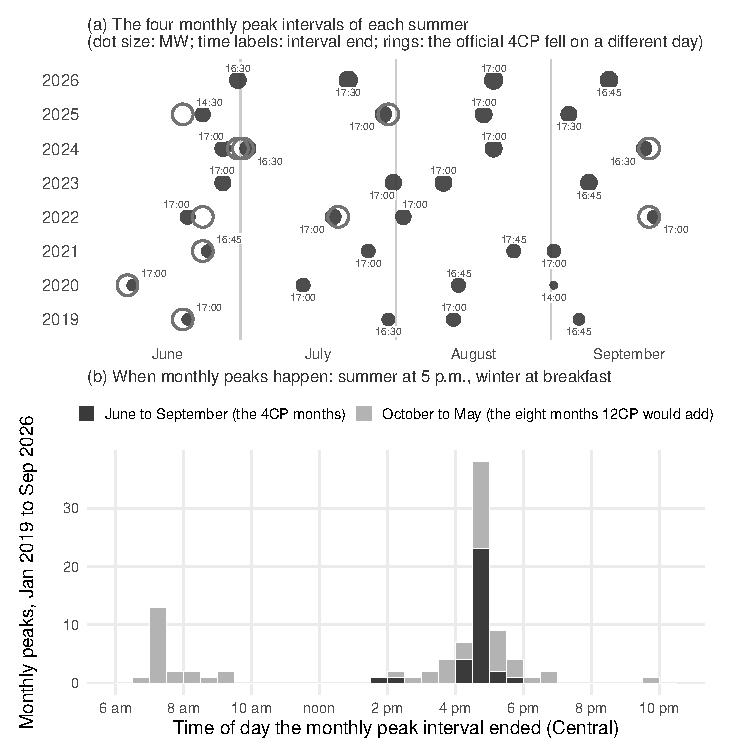
\includegraphics[width=\textwidth]{images/fourcp_calendar}
  \caption{
    (a)~The four monthly peak intervals of each summer since 2019, reconstructed from ERCOT fuel generation as a demand proxy; where ERCOT's official 4CP fell on a different day, a ring marks the official date. Dot size scales with megawatts. (b)~The time of day of every monthly peak from January 2019 to September 2026, the four 4CP months against the other eight: summer peaks cluster at 5~p.m., winter peaks cluster around 7:30~a.m. Generation is net of storage charging, with DC ties omitted and no gap-filling; the official 4CP dates are from ERCOT's annual 4CP workbooks. % fig-src: analysis/figures/fig_ch8_4cp_calendar.R on analysis/data/ercot_monthly_peak_intervals_reconstructed.csv (analysis/checks/ch8_4cp_peaks.R: ercot_fuel_mix_15min_2019on.csv.gz via ch8_demand.R, no gap-fill, complete months) and analysis/data/ercot_official_4cp_2018_2025.csv
  }
  \label{fig:fourcp-calendar}
\end{figure}

Figure~\ref{fig:fourcp-calendar}(a) rebuilds the peaks from ERCOT's Fuel Mix Report: generation summed across fuels, including the battery-charging adjustment, as a generation-based demand proxy \autocite{ercotfuelmixhistory}. It omits net imports over the DC ties and does not separately reconstruct \glossaryterm{block-load-transfer}{Block Load Transfers}: groups of customers disconnected from their usual grid area and connected to a neighboring one \autocite{ercot2026protocols}. In the reports for 2019 to 2021, the battery-charging adjustment sits inside ``Other''; from 2022 it has its own category. Summing all categories includes it in both periods. The proxy already nets out battery charging. Subtracting it again would count the adjustment twice. This is a settlement reconstruction, not a live feed; August and September 2026 are still initial settlement. It matches 17 of the 28 official peak dates in 2019 to 2025, so the official filings remain the authority on which afternoon won. % src: analysis/checks/ch8_4cp_peaks.R console (17 of 28 dates match; 24 of 28 daily peak intervals match the official label; 14 of 28 monthly peak intervals match); analysis/data/fetch_ercot_fuel_mix.py and ercot_fuel_mix_15min_2019on.csv.gz (2019-2021 Summary notes include WSL adjustments in Other; WSL separate from 2022; FINAL through July 2026, INITIAL August-September 2026); ercot2026protocols sec. 2 (Block Load Transfer definition) and sec. 9.17.1(3) for BLT terms; ercotfuelmixhistory

The accounting detail from Section~\ref{sec:fourcp-rule} matters even when watching ERCOT's own live demand number: battery charging counts there and not in the settlement peak. The exclusion dates to February 2013 \autocite{ercotnprr461}. ERCOT reminded participants of this in August 2024 and later confirmed that storage charging and DC-tie treatment moved the winning date in June and September 2024 \autocite{ercot2024mktnotice4cp,ercottwg20254cp}. % src: ercotnprr461 (Board Report 121112, sec. 9.17.1(3); effective 2013-02-14 for this section; independently checked against January 2019 Protocols sec. 9.17.1(3)); ercot2024mktnotice4cp (WSL included in operational load, excluded from settlement 4-CP); ercottwg20254cp (Deviation from Operation Load: WSL and DC-tie treatment, twice in 2024, June and September); these are ERCOT's operational-versus-settlement findings, not an attribution of the fuel-mix proxy's residual errors
A 4CP forecast has to model the settlement definition, batteries subtracted, or it will celebrate the wrong afternoon.

Two more patterns sit in the data. The peaks are climbing: the annual peak in this reconstruction rose from 74.1~GW in 2019 to 91.5~GW on August 20, 2026, the highest through September, and the lowest monthly peak of the year rose from 52~GW in 2019 to 62~GW in 2025. The proxy does not establish an official record: ERCOT's provisional demand record is about 91.2~GW on July 22, 2026 \autocite{ercot2026factsheet}. % src: analysis/checks/ch8_4cp_peaks.R console (2019 peak 74,075 MW; 2026 peak 91,455 MW on 2026-08-20 interval ending 17:00; lowest monthly peaks 52,130 MW in Apr 2019 to 62,392 MW in Dec 2025; 2026 nine complete months only; September 2026 peak 87,187 MW on 2026-09-12 interval ending 16:45, below August); ercot2026factsheet October 2026 edition read 2026-11-01 (91,155 MW on July 22, unofficial until final settlement; was 91,134 MW in the edition read 2026-09-27; mutable PDF)
And the summer peak hour is not moving, while the hour that matters to the grid is. Chapter~6 showed the net-load peak, demand minus wind and solar, sliding into the evening; ERCOT's own summer reviews put it at hour ending 21 (8 to 9~p.m.) in 2023 and 2024 and hour ending 22 in June and July 2025. % src: ercotsummer2025review (net load hour HE 21 -> HE 22); ch6 sec. 6.6 (IMM: tightest hours 7-9 p.m.)
The 4CP interval, which counts gross demand with solar still shining, has stayed at 5~p.m. all along. So the one hour Texas uses to allocate its transmission costs is no longer the hour the system is short of power; ERCOT told its board in 2026 that 4CP ``does not correspond to the system's highest net-load peaks,'' even as it remains the strongest load-reduction incentive in the state \autocite{ercotsummer2025review,ercotboard2026dr}. % src: ercotboard2026dr
Hold that thought for Section~\ref{sec:twelvecp}; I read it as one reason the commission has proposed to rewrite the rule.

\section{What Makes a Peak, and How Hard It Is to Call}
\label{sec:fourcp-factors}

Ask what sets a Texas summer peak and the first answer is weather: afternoon temperature across the big load centers drives air-conditioning, and air-conditioning drives the peak. Weather is necessary but not sufficient, because the peak is a competition between afternoons. A Tuesday at 104 degrees Fahrenheit (40 Celsius) sets the July peak only if no other July afternoon is hotter, or later in the month with more load connected, or less relieved by clouds over Houston. Five factors decide that competition.

The first is the calendar. Load grows within the summer as more equipment is energized, so late-month afternoons carry a structural edge; the table shows peaks clustering late in June and July. The second is the weekday, because the same temperature produces more demand on a workday than a Sunday, which is why 31 of 32 peaks were weekdays and the one Sunday needed a month-end heat wave to break the pattern. % src: analysis/checks/ch8_4cp_peaks.R console
The third is the hour, and here the grid does the forecaster a favor: the gross-demand peak lives at 5~p.m.\ because that is when air-conditioning demand and still-working offices overlap before solar fades, and Figure~\ref{fig:fourcp-calendar}(b) shows how tightly it clusters. The fourth is the settlement accounting just described, batteries and DC-tie flows netted out of the official number. And the fifth is the strangest: the peak is shaped by the people chasing it. ERCOT estimates that on August 18, 2025, the summer's peak day, cryptocurrency mines cut about 3,150~MW and identifiable 4CP response about 1,500~MW at the peak hour, so that the recorded peak of 83,878~MW would have been roughly 88,500~MW without those reductions. % src: ercotsummer2025review slide 10 (83,878 MW HE17; ~3,151 MW crypto reduction; ~1,501 MW 4CP reduction; 88,530 MW estimated without reductions)
Across the years ERCOT has put the load actively dodging 4CP intervals at as much as 4,000~MW in 2021, 3,500~MW in 2023, 2,500~MW in 2024, and 1,500~MW of 4CP response beyond the mining reduction in the August 2025 interval \autocite{ercotsummer2025review,potomac2021som,potomac2023som,potomac2024som,potomac2026somercot}. % src: potomac2021som p. 39; potomac2023som pp. 34-35; potomac2024som pp. 33-34; potomac2026somercot p. 31 (all relaying ERCOT estimates)
The chairman of the Public Utility Commission described the effect from his side of the table: ``you can actually see usage go down because they're chasing that interval'' \autocite{tep2026gleeson}. % src: tep2026gleeson (Gleeson interview, June 2026)
When several gigawatts of load vanish on the afternoons everyone expects to be the peak, the peak sometimes moves to an afternoon nobody expected. The forecast changes the thing it forecasts. Game theorists have started to formalize this. A 2025 preprint from Columbia University models coincident-peak avoidance as a game among flexible loads. It observes that the forecasting literature treats each load as a price-taker and ignores the effect of everyone's response on the peak being predicted. It finds that when the players are flexible enough the equilibrium is a flattened peak, with system demand pushed toward equality across the contested periods, at an efficiency cost that grows with the players' flexibility \autocite{chen2025cpgaming}. % src: chen2025cpgaming (arXiv 2501.02792v5: Sec. I on prediction studies neglecting agents' effect on CP predictions; Theorem 1 and Sec. VI: agents balance system demand across periods at equilibrium; Theorems 5-6: efficiency loss grows with flexibility and cost disparity)
The many near-equal afternoons of 2025 (Figure~\ref{fig:fourcp-window}) are consistent with that equilibrium, although a hot, flat summer could have produced them on its own.

\begin{figure}[htbp]
  \centering
  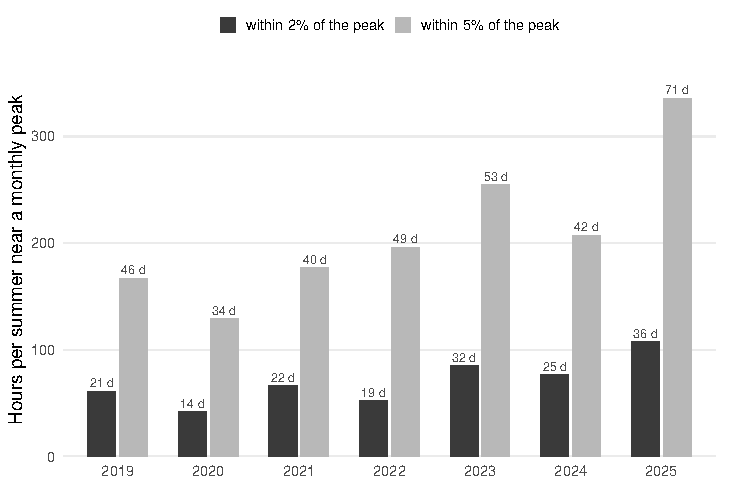
\includegraphics[width=\textwidth]{images/fourcp_window}
  \caption{
    The size of the haystack: hours per summer in which the demand proxy came within 2~percent and within 5~percent of that month's eventual peak, summed over June to September, with the number of distinct days those hours fell on. These are hindsight counts: they assume the height of each peak was known in advance, which in a running season it is not; Table~\ref{tab:fourcp-rules} scores the rules a site can actually run. % fig-src: analysis/figures/fig_ch8_4cp_window.R (summers pinned to 2019-2025) on analysis/data/ercot_fuel_mix_15min_2019on.csv.gz, checked by analysis/checks/ch8_demand.R, no gap-fill
  }
  \label{fig:fourcp-window}
\end{figure}

How hard is the call, then? Figure~\ref{fig:fourcp-window} measures the haystack in hindsight. In a typical summer, 66 hours of 15-minute intervals spread over 22 different days came within 2~percent of one of the four monthly peaks; loosen the tolerance to 5~percent and it is about 196 hours over 46 days. % src: fig_ch8_4cp_window.R console (within 2%: median 66.25 h, 22 days; within 5%: median 196.25 h, 46 days; generation-based proxy, no gap-fill)
2025 was the hardest year in the sample, with 108 hours within 2~percent over 36 days, because a hot, flat summer produced many afternoons of nearly equal height. % src: fig_ch8_4cp_window.R console (2025: 108 h, 36 days within 2%)
Those counts are floors, because they assume the site knew in advance how high the peak would be. In a running season nobody does: the line that defines ``within 2~percent'' is drawn only when the month is over and the tallest afternoon is known.

What a site can actually do without a forecast is run a rule on information it has, and Table~\ref{tab:fourcp-rules} scores four such rules against the 28 official intervals of 2019 to 2025. The clock rules need only the calendar; the demand rules are estimated retrospectively on the demand proxy, which was not available live. % src: analysis/checks/ch8_4cp_rules.R console
Pausing every afternoon from 2 to 6 catches every peak and costs about 490 hours a summer. Pausing weekdays from 4 to 6 costs about 175 hours and lets three of the 28 through: the Sunday peak of June 2024 and two quarter-hours that were over by the time the window opened, the one ending at 2:30 on September 1, 2020 and the one ending at 4:00 on September 20, 2024. % src: ch8_4cp_rules.R console (calendar arithmetic: rule A 488 h every summer, 28 of 28; rule B 172-176 h, median 174, 25 of 28; lets through 2020-09-01 14:15-14:30, 2024-06-30 17:30-17:45 Sunday, 2024-09-20 15:45-16:00)
A threshold on live demand, set against the previous summer's highest peak because that is the only height a site knows in advance, fails in both directions. In the record summers of 2022 and 2023, when June demand already exceeded the previous year's peak, the 95~percent rule idled the site for more than 400 hours. In the milder summers of 2019, 2024, and 2025 it paused about 70 to 75 hours yet caught only one or two of the four peaks, because a mild summer's peaks fall short of last year's and are billed exactly the same. % src: ch8_4cp_rules.R console (C95: 2022 423.5 h and 2023 402.75 h, 4 of 4; 2019 74.25 h 2/4, 2024 71.25 h 1/4, 2025 72.5 h 2/4; C97 caught 15 of 28; threshold tests use the fuel-mix proxy, not an archived live feed)
The honest no-forecast cost of 4CP is therefore not 66 hours but 175 to 490, roughly three to seven times the hindsight haystack, and even the 490 buys certainty only because it pauses through every afternoon of the summer. % src: ch8_4cp_rules.R calendar rules (median 174 h, rule A 488 h); fig_ch8_4cp_window.R median 66.25 h, printed as 66 as in the haystack sentence above: ratios 2.6 and 7.4

\begin{table}[htbp]
  \centering
  \footnotesize
  \setlength{\tabcolsep}{4pt}
  \begin{tabular}{p{5.3cm}rr}
    \hline
    \textbf{Rule, run in real time} & \textbf{Hours paused} & \textbf{Peaks caught} \\
     & \textbf{per summer} & \textbf{of 28} \\
    \hline
    Every day, 2 to 6 p.m. & 488 & 28 \\
    Weekdays, 4 to 6 p.m. & 172--176 & 25 \\
    Live demand at or above 95\% of last summer's highest official peak & 56--424 & 18 \\
    Live demand at or above 97\% of last summer's highest official peak & 8--332 & 15 \\
    \hline
  \end{tabular}
  \caption{Dodging 4CP without a forecast: four rules, with the demand thresholds estimated on a demand proxy rather than a live feed, scored against the 28 official 4CP intervals of the summers 2019 to 2025. Hours are per summer, June through September: calendar arithmetic for the two clock rules, and for the two demand rules a range across the seven summers.} % tab-src: analysis/checks/ch8_4cp_rules.R console (rules A and B from the calendar, cross-checked against the complete demand grid; C95 and C97 on analysis/data/ercot_fuel_mix_15min_2019on.csv.gz checked by analysis/checks/ch8_demand.R, no gap-fill); official intervals from analysis/data/ercot_official_4cp_2018_2025.csv, each scored on its start (label - 15 min, analysis/checks/official_4cp.R): rule B 25, C95 18, C97 15 of 28
  \label{tab:fourcp-rules}
\end{table}

A forecast earns its keep by shrinking that number, and a good one shrinks it a great deal, because the problem has structure: the hour is nearly given, since 30 of the 32 official intervals in Table~\ref{tab:fourcp-official} fall inside one 90-minute window; the weekday is nearly given; and what remains is to judge which few afternoons of a month will stand tallest, which is a question about the whole month's weather and load, not about tomorrow's. % src: analysis/checks/ch8_4cp_peaks.R console (30 of 32 labels in 16:30-17:45, i.e. intervals within 16:15-17:45; 31 of 32 weekdays)
That is why the practical unit of a 4CP forecast is a flagged afternoon rather than a flagged quarter-hour, why a market of forecasting services has grown up around the rule, and why the market monitor can speak of billions spent on the tools. This book does not print a forecast recipe; the commercial ones are private and the good ones are the product. What a reader needs is the shape of the trade: every afternoon flagged costs two hours of margin, every peak missed costs a quarter of a year's transmission charges, so a rational forecast is tuned to warn too often rather than too rarely. The arithmetic of Section~\ref{sec:fourcp-econ} says by how much.

A tempting shortcut is to let the energy price do the forecasting. If the grid's peak were also its scarcest hour, the strike of Chapter~6 would pause the site through the 4CP interval for free. The companion repository tests that against the twenty official intervals of 2021 to 2025. In the Day-Ahead Market the West zone price of the peak hour ranged from \$8 to \$1,553 per megawatt-hour, with a median of \$92; the S19j~Pro's strike of \$72 would have paused the site for eleven of the twenty peaks and the S21~XP's \$157 for six, and all six were in the scarce summers of 2021 to 2023. % src: analysis/checks/ch8_4cp_prices.R console (DAM LZ_WEST at the 20 official 4CP hours, each the hour ending that holds the interval: median $92.47, range $8.29-$1,553.22; >$72: 11 of 20; >$157: 6 of 20, all 2021-2023; data: ercot_dam_spp_loadzones_2021on.csv.gz, ERCOT MIS 13060)
In 2024 and 2025 seven of the eight peak hours cleared below that \$72 strike day-ahead, the eighth at \$94, and the 15-minute settlement point price in the peak interval itself ran from \$6 to \$72, a median of \$29 against a summer average of \$38, crossing the S19j~Pro's strike only once and by under a dollar. % src: ch8_4cp_prices.R console (2024-2025 day-ahead hours: 7 of 8 below $72, highest $94.21 on 2025-07-30 HE17; rtm15 LZ_WEST at the 8 official intervals $6.26-$72.37, median $28.89; one interval above the $71.6 breakeven, 2025-06-19 at $72.37, $0.77 over; Jun-Sep 2024-2025 rtm15 LZ_WEST mean $38.21; real-time prices from ercot_rtm15_spp_loadzones_2021on.csv.gz, ERCOT MIS 13061)
The month's priciest day-ahead hour was the 4CP hour only once, in June 2022, and on thirteen of the twenty peak days the day's priciest hour came later, in the evening. % src: ch8_4cp_prices.R console (month max = 4CP hour in 1 of 20, 2022-06-23 HE17 at $604; day max later than the peak on 13 of 20, at HE 19-21; month-max hours HE 16-17 in 7 of the 8 months of 2021-22, HE 20-21 in 7 of the 8 of 2024-25)
This is the pattern of Chapter~6 seen from the other side: batteries and solar have pushed scarcity from 5~p.m.\ to 8 or 9, while the gross-demand peak that 4CP bills has stayed at 5. The price is no longer a 4CP indicator. A site that pauses only on price runs straight through the quarter-hours that cost it the most, so a 4CP strategy has to watch demand; Chapter~9 prices that interaction.

\section{The Price of Being Wrong}
\label{sec:fourcp-econ}

A miner weighing 4CP faces an asymmetric bet. Each of the four intervals is worth, at retail, \$10,000 to \$17,000 per megawatt of load kept off the meter at transmission voltage. % src: sec. 8.1 transmission-service riders eff. Sept. 1, 2025 / 4: $10,185.65 (Oncor, oncor2026retailtariff) to $16,671.48 (CenterPoint, centerpoint2025tcrf58178)
Each hour of pausing costs the mining margin of Chapter~4: at the 2025 average hashprice and power price, roughly \$30 per megawatt-hour for the S19j~Pro and \$115 for the S21~XP, the difference between what a megawatt-hour earns and what it costs. % src: ch4 breakevens $71.6 (S19j Pro) and $156.5 (S21 XP) per MWh of revenue at 2025 mean hashprice, minus the $42.18 mean settlement price
Take the crude rules of Table~\ref{tab:fourcp-rules}. Pausing every weekday from 4 to 6, about 175 hours, costs roughly \$5,200 per megawatt for the summer on the old fleet and \$20,000 on the new one, against a prize of about \$41,900 per megawatt-year, Oncor's rider since August 2026 and near the bottom of the range above: eight times over for the old fleet, twice over for the new, with three peaks in seven summers let through. % src: 174 h x $30 = $5,220; 174 h x $115 = $20,010; prize floor = Oncor TCRF annualized $41,901 (oncor2026retailtariff); 41,900/5,220 = 8.0x; 41,900/20,010 = 2.1x; ch8_4cp_rules.R (rule B misses 3 of 28)
Pausing every afternoon from 2 to 6, about 490 hours, catches every peak and costs \$14,600 on the old fleet, still a threefold return, but \$56,000 on the new one, more than the prize itself. % src: 488 h x $30 = $14,640 (2.9x); 488 h x $115 = $56,120 (0.75x)
Pausing through only the 66 hours of the hindsight haystack would have cost \$2,000 or \$7,600 of margin; everything between that floor and the brute-force ceiling is the value of knowing which afternoons matter. % src: fig_ch8_4cp_window.R median 66.25 h x $30 = $1,987.50; x $115 = $7,618.75
An S19j~Pro fleet can afford to dodge 4CP by brute force; an S21~XP fleet cannot, and has to buy or build the knowledge that turns 490 hours into a few dozen. The penalty for a false alarm is two hours of margin, \$60 to \$230 per megawatt; the penalty for a miss is a quarter of a year's transmission charges, \$10,000 to \$17,000. % src: false alarm 2 h x $30 = $60 (S19j Pro), 2 h x $115 = $230 (S21 XP), the margins of chapter-8.tex:143 (sec. 8.4; ch4 breakevens $71.6 / $156.5 minus $42.18); miss = one of the four intervals = annual charge / 4 (oncor2026retailtariff sec. 6.1.1.1.7, the average of the four): sec. 8.1 transmission-service riders eff. Sept. 1, 2025, $10,185.65 (oncor2026retailtariff) to $16,671.48 (centerpoint2025tcrf58178)

It also prices the exit from a reserve commitment left open at the end of Chapter~7. Under the old ancillary rules, a reserve award held a site on the meter through a suspected peak afternoon, and the site had to choose between the two revenue streams. Under RTC+B a load can buy out of its ancillary position at the real-time price and pause. No real-time ancillary price existed before December 2025, so the day-ahead clearing price has to stand in for it. Priced that way on the twenty official 4CP afternoons of 2021 to 2025, a two-hour buyout would have cost under \$160 per megawatt on fourteen of them and between about \$660 and \$3,200 on the six tightest, all in the scarce summers of 2021 to 2023, against a transmission stake of \$10,000 to \$17,000 per interval. The peak wins every time, and the ancillary income for the rest of the day is unaffected. % src: ch7 sec. 7.7 (RTC+B financial AS positions; imbalance settled at RT MCPC, which did not exist before Dec 2025, so DAM MCPC is the proxy); fig_ch7_as_history.R console (priciest product's DAM MCPC summed over the two hours holding each official 4CP interval, HE 17-18 on 19 dates and HE 16-17 on 2024-09-20, whose interval 15:45-16:00 falls in HE16: median $74/MW; 14 of 20 days under $160; 6 days $659-$3,168: 2021-07-26, 2022-06-23, 2022-07-20, 2023-07-31, 2023-08-10, 2023-09-08); stake = sec. 8.1 transmission-service riders eff. Sept. 1, 2025 / 4, $10,185.65 (oncor2026retailtariff) to $16,671.48 (centerpoint2025tcrf58178)
Reserve income and 4CP avoidance can now be combined by paying the cost of exiting the reserve commitment.

The system-level view is less flattering. Spread over every megawatt-hour Texans consume, the transmission bill that 4CP allocates came to about \$10 per megawatt-hour in 2024, and to \$8 or \$9 in inflation-adjusted terms in every year since 2021; the figure is ERCOT's own, the year's transmission cost of service divided by the year's energy use, and the market monitor quotes it to size the game. % src: potomac2024som p. 33 ("approximately $10 per MWh in 2024", fn. 29 -> ERCOT Report on Existing and Potential Electric System Constraints and Needs, Dec 2024); potomac2026somercot p. 31 ("$8 to $9 per MWh in inflation-adjusted terms since 2021", fn. 16 -> ERCOT constraints-and-needs report Dec 2025, p. 9: "TCOS per Total MWh Energy Use", CPI-adjusted; TCOS from ERCOT's Yearly Wholesale Transmission Service Charges, MWh from ERCOT's Demand and Energy Report); nominal cross-check 2025: $5,446,864,795 / 488.1 TWh (analysis/checks/ch8_4cp_peaks.R console, the generation-based proxy summed) = $11.16/MWh
Set beside the \$42 average settlement price of 2025, transmission adds roughly a quarter on top of energy for a load that pays its full share, and the monitor's point is that the loads best placed to avoid that quarter, ``operationally flexible loads, such as cryptocurrency mines,'' shift a disproportionate share of it onto everyone else. % src: $10-11/MWh vs $42.18/MWh = 24-26% ($11.16/$42.18 = 26%); potomac2026somercot pp. 132-133 (quote)
In its report on 2024 the monitor wrote that ``billions of dollars have been spent on developing 4CP forecasting tools and installing behind-the-meter generation, creating vested interests in maintaining the current structure,'' and in the following year's report that pausing during intervals that no longer coincide with real scarcity suppresses the very price signals the energy-only market depends on \autocite{potomac2024som,potomac2026somercot}. % src: potomac2024som p. xxvii (verbatim quote); potomac2026somercot p. 31 (4CP response weakens scarcity pricing)

\section{From Four Peaks to Twelve}
\label{sec:twelvecp}

In June 2025 Texas enacted Senate Bill~6, its answer to a wave of proposed data centers and other large loads that had ERCOT planning for a 2030 peak of 130 to 148~GW, existing load included, against a 2024 peak of about 85~GW \autocite{texas2025sb6,texassrc2025sb6,ercot2025ltlf}. % src: ercot2025ltlf slides 10-11 ("130 GW to 148 GW range used in 2024 Regional Transmission Plan for forecast year 2030", a TOTAL peak: the ERCOT-adjusted 2030 peak is 138 GW with 94,145 MW of base load included; potomac2026somercot p. viii reads it the same way, 138-148 GW, 62-74% over the current peak); texassrc2025sb6 (statement of intent; as recorded when accessed, it gives the range as 130-150 GW of additional load against an 86 GW 2024 peak, which ERCOT's own slide shows is the total 2030 peak; not re-read at origin 2026-09-26, capitol.texas.gov resets connections from this network); 2024 peak 85,357.56 MW, the official August 2024 4CP interval (analysis/data/ercot_official_4cp_2018_2025.csv, NP9-83-M), below the 85,508 MW record of August 10, 2023 (ercot2026ltlfprelim); texas2025sb6 (signed and effective June 20, 2025)
Most of the bill is about interconnection: a load that asks for a new or expanded connection bringing one site to 75~MW or more faces new standards and a study fee of at least \$100,000, and must disclose its backup generation. If that backup could carry half its demand, the load can be directed by ERCOT to run it or curtail once every market service short of frequency response has been exhausted, under an emergency threshold ERCOT had not yet set by September 2026 \autocite{puct2026order58481,ercot2026sb6status}. And for any transmission-connected load interconnected after 2025, other than critical-load industrial customers and critical natural gas facilities, the wires utility must have a protocol, and any equipment it needs, in place before the load connects, so that the load can be curtailed during firm load shed, the rolling blackouts of Chapter~2. % src: texas2025sb6 sec. 2 (PURA 37.0561: 75 MW threshold; backup generation >= 50% of on-site demand; directed deployment or curtailment; $100,000 study fee) and sec. 4 (PURA 39.170(a): a firm-load-shed protocol, with any necessary equipment, for loads interconnected after Dec 31, 2025; excludes critical load industrial customers per PURA 17.002 and critical natural gas facilities per PURA 38.074); PURA 37.0561(c): the standards "must apply only to customers requesting a new or expanded interconnection where the total load at a single site would exceed" the threshold, and (e)-(f) tie the backup-generation disclosure, directed deployment and study fee to customers "subject to Subsection (c)"; (e): ERCOT "shall establish a threshold before or during an energy emergency alert" for the notice, and only customers with on-site backup generating facilities, generation that "can serve at least 50 percent of on-site demand", may be directed; puct2026order58481 25.194(f)(1)(G), order p. 249 (a large load customer discloses whether it has or plans "backup generating facilities or on-site backup generating facilities", the first defined in 25.194(c)(2) with no size condition; effective October 8, 2026); ercot2026sb6status slides 6-7 (September 2026: "Establish a threshold before or during an EEA ... to be effective after adoption of PUC rule" In Progress, completion TBD; operating procedures for curtailing loads with backup "serving at least 50% of customer load" In Progress; the process to receive the backup disclosures Not Started); PURA 39.170(a): the commission "shall require" ERCOT to ensure that each utility serving a transmission-voltage customer "develops a protocol, including the installation of any necessary equipment or technology before the customer is interconnected, to allow the load to be curtailed during firm load shed"
That last duty is written into the statute but not yet into a commission rule: the rule the commission proposed in July 2026 for the demand management service described below repeats the statute's words without naming the equipment \autocite{puct2026prop58482,puct2026sb6roadmap}. % src: puct2026prop58482, proposed 25.521(a)(1) (filed July 30, 2026; restates PURA 39.170(a) as a directive to ERCOT; names no equipment or method); puct2026sb6roadmap (Project 58482 "restyled for possible implementation of PURA 39.170(a) in addition to PURA 39.170(b)"; recommended adoption order at an open meeting in January 2027, the date the demand-management-service line in sec:programs prints); no commission order implementing 39.170(a) in the 58482 filings through September 6, 2026, and adopted 25.194 (puct2026order58481) has no firm-load-shed provision
For a stand-alone site of 75~MW or more connecting at transmission voltage, ERCOT's own interconnection rules already require breakers the transmission operator can open remotely \autocite{ercotplanningguide2026,ercot2026protocols}. % src: ercotplanningguide2026 Sec. 9 (effective July 11, 2026) 9.2.5(1) (a Large Load not co-located with generation, interconnected at transmission voltage: breakers "under the remote control of the applicable Transmission Operator (TO)"); 9.2.5(2): a load co-located with generation uses breakers "remotely controllable at the direction of the applicable" QSE; ercot2026protocols sec. 2 (Large Load: aggregate peak Demand "greater than or equal to 75 MW"); ERCOT's "89th Legislative Session - ERCOT Status" deck, June 2026, slide 10, frames the 39.170(a) work as deciding "whether additional breaker requirements beyond those in Planning Guide Section 9.2.5 are needed"
Section~6 of the bill is the one that matters here. It ordered the commission to evaluate ``whether the current four coincident peak methodology \ldots\ ensures that all loads appropriately contribute'' to transmission costs, to consider ``multiple seasonal peak demands, demand during different length daily intervals, or peak energy intervals,'' and to amend its rules by December 31, 2026. % src: texas2025sb6 sec. 6(a)(1)-(2), (c)

The commission's staff studied the question through the winter and reported in March 2026 with a list of shortcomings that reads like a summary of this chapter. Among them: the four summer intervals miss winter scarcity entirely; fifteen minutes is too narrow a window to send a fair signal; sophisticated large consumers can predict the intervals and cut load in time; and the arrival of flexible large loads, ``such as crypto mines and certain types of data centers,'' will make clean cost assignment harder every year \autocite{puctstaff2026draftreport}. % src: puctstaff2026draftreport (Project 58484, Item 77, memo p. 2 and report pp. 5-6, 17; coins "CP-Incentivized Demand Reduction")
The proposal that followed was published in the Texas Register on July 24, 2026, and it does three things. % src: puct2026prop58000 (filed July 9, 2026; published July 24; comments due August 11)
It replaces 4CP with \glossaryterm{12cp}{12CP}: twelve monthly peaks, one for every month from October through September, each measured over a thirty-minute interval instead of fifteen. % src: puct2026prop58000, proposed 25.192(b)(4) ("The set of 12 30-minute intervals composed of the ERCOT system monthly peak demand interval for each of the 12 calendar months from October 1 ... through September 30")
It creates a \glossaryterm{minimum-billing-demand}{minimum billing demand} for the loads the commission's new large-load interconnection rule covers (a new site of 75~MW or more, or the added megawatts of an expansion that first takes a site to 75~MW or adds 75~MW or more to one already past it). The minimum is the greater of the peak demand written into its service contract, its highest demand in the past year, or its 12CP demand, billed for at least twenty years whether or not the site consumes. The wires utility adds the same megawatts to its own wholesale bill, so the transmission owner is paid in full. % src: puct2026prop58000, proposed 25.193(d)(1) (applies to "a large load customer, as determined by 25.194"), 25.193(d)(2)-(3) (greater of contracted peak, prior-year NCP, or 12CP demand; no less than 20 years), 25.192(b)(6) (large load customer = "An entity that is subject to 25.194") and 25.192(f)(1)(B) (DSP 12CP load grossed up by the gap); puct2026order58481, adopted 25.194(b)(1)(A)-(D) and (b)(2), order p. 224 ((B) an expanded interconnection at a single site that equals or exceeds 75 MW for the first time, (C) one at a site that exceeds 75 MW and is expanding by 75 MW or more, (b)(2) for an expansion the section applies to the incremental load addition; in full: a large load customer not energized as of the section's effective date that seeks a new interconnection of 75 MW or more at a single site, an expansion reaching 75 MW for the first time, an expansion of 75 MW or more at a site already above 75 MW, or co-location with a generation resource; for an expansion, only the incremental load) and 25.194(c)(14), order p. 227 (large load customer = "An entity requesting a new or expanded interconnection")
A site already energized when that rule takes effect on October 8, 2026, and not expanding, is outside the minimum as proposed \autocite{puct2026prop58000,puct2026order58481}. % src: puct2026order58481 adopted 25.194(b)(1)-(2) and Item 219 (Texas Register acknowledgment TRD-202604027: "Effective Date: 10/08/2026"); puct2026prop58000 25.192(b)(6), 25.193(d)(1); contested in the Project 58000 comments, hence "as proposed": the Texas Blockchain Council (Item 41) asks the commission to grandfather energized loads, American Bitcoin (Item 14) to confirm the new-or-expanded scope in the rule text, and OPUC (Item 63) to reach existing customers seeking to expand
And it asks, in so many words, whether ``large computational load'' such as data centers and cryptocurrency mining facilities should receive separate rate treatment altogether \autocite{puct2026prop58000}. % src: puct2026prop58000 (question on separate rate treatment for large computational load, >= 50% power-electronic load)
Comments closed on August 11, 2026. The statute requires final rules by the end of the year, the commission's staff plans to bring its recommended rule in December, and as proposed the new billing determinants would take effect with the first annual transmission-charge docket that uses ERCOT's 12CP data \autocite{puct2026sb6roadmap}. % src: puct2026prop58000 (comments due August 11, 2026; transition rule 25.192(l)(1)); texas2025sb6 sec. 6(c) (December 31, 2026); puct2026sb6roadmap (Project 58000: 909 pages of comments to synthesize; recommended adoption order at an open meeting in December 2026)
The chairman was candid about the intent: ``a minimum demand ratchet, so that you couldn't avoid all or most of your transmission costs'' \autocite{tep2026gleeson}. % src: tep2026gleeson

Read against this chapter's data, the reform as proposed lands in two very different places. For a new load of 75~MW or more, and for the added megawatts of an expansion the rule covers, the game would be over. The minimum billing demand bills at least the contracted capacity regardless of what the meter shows, so a new data center or mine of that size pays for every megawatt in its service contract whether it runs or pauses. Transmission becomes what it is for every other industry, a fixed cost. The commission has itself asked whether that minimum should instead step down in phases over the twenty years, be set at a percentage of the contracted demand, or be averaged with the site's 12CP demand, and any of the three would hand part of the game back \autocite{puct2026prop58000}. % src: puct2026prop58000, questions for comment (minimum billing demand "fixed for 20 years as proposed", "reduced in phases over a period of 20 years", or "extended to a longer time period"; a "ratcheted" demand, "some percentage of the customer's contracted peak demand or maximum NCP demand in the previous year"; a "weighted average" of contracted peak or highest NCP demand and 12CP demand)
For a smaller site, and for a large one already running before the rule, the game continues but changes shape. There are twelve peaks to cover instead of four, eight of them in months 4CP never counted. Figure~\ref{fig:fourcp-calendar}(b) shows what they look like: 34~percent of the reconstructed non-summer monthly peaks since 2019 fell between 6 and 10 in the morning, the winter breakfast peak of a Texas cold snap, including 80.7~GW at 7:30 on the morning of February 20, 2025 and 77.7~GW on the morning of January 16, 2024. % src: analysis/checks/ch8_4cp_peaks.R console (non-summer peaks: 34% in HE 7-10; 2025-02-20 07:30 80,697 MW; 2024-01-16 08:45 77,707 MW)
A winter morning peak is a different forecasting problem, driven by heating and pre-dawn cold rather than afternoon heat, and a thirty-minute interval is easier to hit but longer to sit out.

The arithmetic changes with the count. The same annual charge spread over twelve peaks makes each one worth a third as much: about \$3,500 per megawatt at the Oncor floor instead of \$10,500. % src: analysis/checks/ch8_12cp_haystack.R console ($41,901 / 12 = $3,492; / 4 = $10,475)
The hindsight haystack for a twelve-month year, counted in the same thirty-minute intervals, runs 64 to 143 hours within 2~percent of the monthly peaks, a median of about 105. So a site that paused only through those hours would still come out well ahead, about \$3,100 of margin on the old fleet and \$12,000 on the new for the same \$41,900. % src: ch8_12cp_haystack.R console, clock half-hour haystack (Oct-Sep years 2020-2025: 63.5-143 h within 2%, median 104.5; 104.5 x $30 = $3,135; x $115 = $12,018); 15-minute basis 61.5-131.75 h, median 101.75 ($3,052 and $11,701); peaks reconstructed from the fuel-mix proxy
But more than a third of the eight added peaks fall in the morning. A rule crude enough to run without a forecast (a weekday window at breakfast and another at 4~p.m.\ in every month of the year) would idle the site for about 1,040 hours and still cover only eight to eleven of the twelve reconstructed thirty-minute peaks: \$31,000 of margin on the old fleet, \$120,000 on the new, for at most eleven twelfths of a \$41,900 prize. % src: ch8_4cp_peaks.R console (non-summer peaks: 34% in HE 7-10, 51% in HE 17-21); ch8_12cp_haystack.R console (weekdays 07-09 and 16-18, all months: 1,040-1,048 h; 8-11 of 12 monthly peaks covered, scored on clock half-hours as proposed 25.192(b)(4) measures them (10, 8, 8, 8, 10, 11 in Oct-Sep 2020-2025; 8-10 on 15-minute peaks), 11/12; 1,040 x $30 = $31,200; 1,040 x $115 = $119,600)
For the new fleet that is a plain loss, about a quarter of the outlay coming back. For the old one, at that flat margin, it is roughly a wash: the peaks covered are worth 1.02 times the margin given up, a little ahead in three of the six years. Price the pause interval by interval at 2025's hashprice instead, so that the hours the strike already sits out cost nothing and every other hour costs the margin it would earn at that hashprice, and even the old fleet falls behind in every year from 2022. At each day's own hashprice, the basis of this chapter's closing ledger, it falls behind in those same years. % src: ch8_12cp_haystack.R console, two-window rule (Oct-Sep 2020-2025, 30-minute proxy peaks covered x $3,492): flat margins $30/$115, S19j Pro 1.02x overall, ahead in 3 of 6; S21 XP 0.27x, ahead in 0 of 6; strike at 2025 breakevens $71.6/$156.5, S19j Pro 2022-2025 0.91x, 0.71x, 0.76x, 0.94x (0.82x overall), S21 XP 0.23-0.31x; own-day hashprice S19j Pro 0.13x, 0.43x, 0.48x, 0.85x. On 15-minute peaks S19j Pro 1.00x flat and 0.80x strike; proxy peaks are not official 12CP determinations
Under 12CP brute force at best breaks even, and what is left of the game belongs to sites outside the minimum billing demand, smaller than 75~MW or already running before it, that hold a forecast good enough to turn a thousand hours into a hundred. The market monitor, for its part, would go further than the commission, and has argued for allocating transmission costs by annual energy share or by a predetermined number of floating one-hour coincident peaks across the year. The first would end the game entirely for everyone; the second would only make it harder to play. % src: potomac2026somercot pp. 132-133 (annual load ratio share; hybrid: a portion of T-COS on a predetermined number of floating one-hour coincident peaks)
Whichever version prevails, my reading is that the 4CP rule this chapter opened with is in its last summer or two, and the numbers in Table~\ref{tab:fourcp-official} are a record of an era.

\section{Programs Beyond Price}
\label{sec:programs}

Price arbitrage and 4CP avoidance share a logic: the load watches a number and acts on its own. The ancillary services of Chapter~7 pay a load for a promise, but they are bought in a market that clears every five minutes beside energy, and they are deployed as a matter of routine. ERCOT also runs programs outside that market: a load contracts months ahead, from a budget the commission caps by rule, to act on ERCOT's call in a declared emergency, and it is paid for the promise whether or not the call ever comes. The largest is the \glossaryterm{emergency-response-service}{Emergency Response Service} (ERS), a contracted reserve of last resort deployed when the grid's operating reserves fall below 3,000~MW or an emergency is declared, that is, after the ancillary services of Chapter~7 have already been used \autocite{puct25507,ercot2026protocols}. % src: puct25507(b) (ERS established by commission rule); ercot2026protocols sec. 6.5.9.4.1(2), "General Procedures Prior to EEA Operations": "When PRC falls below 3,000 MW and is not projected to be recovered above 3,000 MW within 30 minutes following the deployment of Non-Spin, ERCOT may deploy available contracted ERS-10 and ERS-30 via an XML message." This is a step taken before EEA Level 1 is declared, not an EEA Level 1 step; NPRR1238 replaces the paragraph on system implementation to add "and all VECL". Attachment Q says nothing about deployment triggers, so ercotattq2025 is dropped from this line.
Its budget is capped by rule at \$75~million a year, plus up to \$25~million for renewals in an emergency; ERCOT procures it four times a year in seasonal terms, in ten-minute and thirty-minute varieties, through a clearing-price auction with an offer cap of \$80 per megawatt per hour \autocite{puct25507,ercot2026protocols,ercotattq2025}. % src: puct25507(b)(2) ($75M + $25M); ercot2026protocols sec. 3.14.3.1(1) (four ERS Standard Contract Terms: Dec-Mar, Apr-May, Jun-Sep, Oct-Nov), sec. 3.14.3.1(2) (four ERS service types: weather-sensitive and non-weather-sensitive ERS-10 and ERS-30); ercotattq2025 sec. C ($80/MW/hr offer cap), sec. F (highest accepted offer sets the clearing price for all service types)
It is a capacity payment for availability, with no extra payment when called, and the obligation is bounded: at most 24 cumulative hours of deployment in a winter contract period and 12 in the others \autocite{ercot2026protocols}. % src: ercot2026protocols sec. 3.14.3.1(17)(b) (24 hours of cumulative deployment time for any ERS Contract Period in the December through March Standard Contract Term, 12 hours in all other Standard Contract Terms), sec. 3.14.3.1(22) (deployment brings no additional payment beyond Real-Time energy imbalance or other settlement)
It is also rarely used: ERCOT counts eleven deployments in the program's eighteen years, about one every twenty months, the last in September 2023. A resource's ERS capacity may not be committed to any ancillary service, to real-time dispatch, or to a utility program at the same time \autocite{ercotgridinsightsdr2025,ercot2026protocols}. % src: ercotgridinsightsdr2025 (11 deployment events in 18 years = one per 19.6 months; the IMM's 2025 SOM counts nine since inception, ERCOT's own count is used); potomac2026somercot p. 32 (most recent deployment September 2023); ercot2026protocols sec. 3.14.3.1(11)(f) (offer must affirm that no offered capacity is committed to any other product, service or program during the ERS Time Period, incl. Ancillary Services, SCED, TDSP standard offer programs)

Miners found it, in numbers. Chapter~7 left them deregistering as Controllable Load Resources (CLRs) in 2025; ERS is where they went. For the 2025 program year ERCOT procured an average of about 1,700~MW every hour, 45~percent more than the year before, at an average clearing price of \$4.36 per megawatt per hour, 41~percent less; cryptocurrency mines were about 56~percent of the volume by summer 2025 and more than 64~percent by spring 2026 \autocite{potomac2026somercot}. % src: potomac2026somercot p. 32 (1,666 MW/h, +45%; $4.36/MWh, -41%; 56% summer 2025; >64% spring 2026)
The market monitor's objection is precise, and it will shape the program's future: paying a price-sensitive miner to stand by ``essentially pays them to do what they would already do, i.e.\ curtail when system conditions are tight and energy prices are high,'' while removing them from the real-time dispatch where, as CLRs, they were visible to the operator; the monitor wants the eligibility rules changed to push them back. % src: potomac2026somercot p. 32

The monitor's phrase describes the emergency hour, when prices sit at the cap and a mine would be off in any case. It does not describe the rest of the contract, and there the program asks for the opposite of what this chapter has been recommending. ERS is sold by time period: eight standing blocks, five of them weekday daytime and evening hours, two for weekends and holidays, and one for everything left over. A load commits to whichever blocks it chooses for the whole term. % src: ercotersreq2026 (standing ERS Time Periods, June-September 2026 term: weekdays HE 06-09, 10-13, 14-16, 17-19, 20-22; weekend and ERCOT holiday HE 06-09 and 16-21; Time Period 8 = all other hours)
The fourth block is weekdays from 4 to 7 in the afternoon, and 29 of the 32 official 4CP intervals in Table~\ref{tab:fourcp-official} fall inside it. % src: analysis/checks/ch8_4cp_peaks.R console, ERS Time Period 4 line (weekday, not an ERCOT holiday, interval inside 16:00-19:00 CPT): 29 of 32; outside are 2020-09-01 14:15-14:30 and 2024-09-20 15:45-16:00, both in Time Period 3, and Sunday 2024-06-30, a weekend block
In every committed quarter-hour of a block it has sold, ERCOT reads the meter, and a load consuming less than 95~percent of the capacity it contracted is counted unavailable for that interval, whatever the reason. % src: ercot2026protocols sec. 8.1.3.1.3.1(1)(a)(i) (ERS Load on a default baseline is unavailable for any 15-minute interval in which its interval Load was less than 95% of its contracted ERS MW capacity; ERSAF = available intervals divided by intervals in the Time Period; loads on the alternate baseline are scored proportionally on average Load); (1)(c) excludes intervals of an actual deployment or test
That is the catch the market monitor's sentence passes over. A mine that pauses for a price spike or a suspected peak has nothing left to shed, so the very hours it most wants to be dark are hours it is paid to be lit; the rules carve out only real deployments and tests, so a price-driven pause counts against the load. % src: ercot2026protocols sec. 8.1.3.1.3.1(1)(a),(c)
The penalty is graduated rather than absolute. The availability factor sets the availability component of the payment, so each missed interval costs its own share, and only when a QSE's whole portfolio falls below 95~percent for the contract period can ERCOT suspend the QSE and its resources for a term and refer it to the commission for penalties \autocite{ercot2026protocols,ercotersreq2026}. % src: ercot2026protocols sec. 8.1.3.3.3(iii) (portfolio availability factor determines the availability component of the ERS payment and whether requirements are met), sec. 8.1.3.3.1(1)-(3) (>= 0.95 = met; otherwise suspension for one Standard Contract Term and possible PUCT administrative penalties; within a failing portfolio a resource below 0.85 has its factor squared); ercotersreq2026 (Unavailability Submission Form; notice required for a material reduction, defined as 25 MW or more for more than 72 hours)
But the slack is thinner than it sounds. A summer term on that afternoon block runs to 255 obligated hours on ERCOT's count, so 5~percent of it is under 13 hours, and pausing through four perfect 4CP afternoons for three hours each spends 12 of them. % src: ercotersproc2025 (June-September 2025 non-weather-sensitive ERS-30, Time Period 4: 255 h = 85 weekdays, the 87 of the term less the ERCOT Holidays July 4 and September 1, 2025, x 3 h, HE 17-19; reproduced from the ERCOT Holiday calendar by analysis/checks/ch8_ers_blocks.R); 5% = 12.75 h; 4 x 3 h = 12 h = 4.7%
A forecast that raises any false alarm, as every forecast does, goes straight through the line, and the price strategy of Chapter~5 would go through it in a single week.

So the afternoon ERS block and 4CP avoidance are best kept apart, and the prices show why. In the summer of 2025 the afternoon block cleared at \$18.69 per megawatt per hour, the term's highest price and four times the program's average, and paid about \$4,800 per megawatt for the term \autocite{ercotersproc2025}; one 4CP interval is worth \$10,000 to \$17,000. % src: analysis/checks/ch8_ers_blocks.R console on ercotersproc2025 (June-September 2025 non-weather-sensitive ERS-30 Time Period 4: 255 h x $18.69 = $4,766/MW; the highest of the term's eight Time Periods, Time Period 5 next at $18.08; $18.69 / $4.36 = 4.3x the potomac2026somercot p. 32 program-year average; the dearest block of the program year was the December-March weekday breakfast block, $26.87); per-interval value = sec. 8.1 transmission-service riders eff. Sept. 1, 2025 / 4, $10,185.65 (oncor2026retailtariff) to $16,671.48 (centerpoint2025tcrf58178)
A mine forced to choose pauses and eats the availability loss, and a mine thinking one step ahead never sells that block at all: it commits the early mornings, the weekend blocks, and the leftover hours, and keeps its afternoons free. On the 2025 clearing prices those blocks paid about \$18,000 per megawatt for the year, half of it the winter breakfast block, but only to megawatts the price seldom stops. The S19j~Pro's strike was crossed in more than 5~percent of the hours of every one of those blocks, and in a fifth of the winter breakfast block; the S21~XP's in 4~percent at worst. % src: analysis/checks/ch8_ers_blocks.R console on ercotersproc2025 (December 2024-November 2025, non-weather-sensitive ERS-30, per MW: Time Periods 1, 6, 7 and 8 of the four terms = $17,948, of which December-March Time Period 1 (weekdays HE 06-09) $8,813 = 49%); part 3: share of each block's quarter-hours with the LZ_WEST 15-minute settlement point price above the strike at the previous day's hashprice (29.5 and 13.5 J/TH), S19j Pro above 5% in all 16 of those blocks, 20.9% in December-March Time Period 1, S21 XP at most 4.2% (the same block), 0.9% over the four; availability test ercot2026protocols sec. 8.1.3.1.3.1(1)(a)(i)
ERCOT's own numbers say the mine that pauses anyway is common. Its staff found that 60~percent of ERS resources had already self-deployed before the deployment instruction of September 6, 2023, cutting load on the high prices that preceded the emergency. The consultants who reviewed the program for ERCOT's board in April 2026 warned that this gives operators ``a false sense of security'' about what is left to call on, pushes ERS prices toward zero, and may need protocol reforms and claw-back provisions to fix \autocite{ercotboard2026dr,ercotgridinsightsdr2025}. % src: ercotboard2026dr, appended CRA assessment (ERCOT WMS Jan 7, 2026, Agenda Item 4 "ERS/Crypto Mining Load", at 5: 60% of ERS resources self-deployed before the Sept 6, 2023 instruction; CRA sec. 6.1: "false sense of security", "not a good use of customer funds", "may require ERCOT Protocol reforms", claw-back provisions); WMS draft minutes Jan 7, 2026 (concerns raised on crypto maximum base Load, baselines, "early deployment by Loads"); ercotgridinsightsdr2025 p. 2
Senate Bill~6 adds a new emergency product alongside ERS, a large-load demand management service for sites of 75~MW or more with 24 hours' notice, and bars from it any load that already curtails in response to price or sells another reliability or ancillary service. The proposed rule caps offers at \$5,000 per megawatt-hour and extends the exclusions to ERS and the utility programs: a demand-response service written, in effect, for the loads that do not already respond \autocite{texas2025sb6,puct2026prop58482}. % src: texas2025sb6 sec. 4 (PURA 39.170(b)); puct2026prop58482 (Project 58482; 75 MW; 24-hour notice; $5,000/MWh cap; ineligibility for price-responsive, AS, ERS, and TDSP program participants)
Comments on it closed in September 2026, and the commission's staff plans to bring it for adoption in January 2027, so its cap and its exclusions may still change \autocite{puct2026sb6roadmap}. % src: puct2026prop58482 (comments due September 4, 2026); puct2026sb6roadmap (Project 58482: comments received September 4, 2026, 341 pages to synthesize; recommended adoption order at an open meeting in January 2027); no adoption in the 58482 filings through September 6, 2026

Below ERCOT sit the wires utilities' own load-management programs, paid from energy-efficiency budgets and aimed at commercial sites: Oncor offers up to \$35 per kilowatt of summer afternoon (1 to 7~p.m.) reduction on thirty minutes' notice, CenterPoint \$40 per kilowatt of verified curtailment for up to four events of four hours \autocite{oncor2026clmsop,centerpoint2025clm}. % src: oncor2026clmsop ($35/kW max, 100 kW minimum, 30-minute notice, June 1 to Nov 30 with 1-7 p.m. peak); centerpoint2025clm ($40.00/kW; 50 kW minimum; up to 4 curtailments of up to 4 h plus 2 tests)
They are small and hemmed in: budgets of a million dollars or so, exclusions for load already paid by any ERCOT program, and in Oncor's case for any for-profit load served at transmission voltage, which rules out every mine of the size this book discusses. % src: oncor2026clmsop (2026 incentive budget $1,000,000; excludes ERCOT-program load and transmission-voltage for-profit load)
For a small site behind a distribution feeder they can be another stream; for a large one they are not on the menu.

\section{How a Site Actually Signs Up}
\label{sec:aggregators}

Every ERCOT program in this chapter and the last shares one door. A load cannot deal with ERCOT directly; it is represented by a Qualified Scheduling Entity (QSE), the licensed intermediary of Chapter~7, and ERS offers in particular may be submitted only by a QSE, on the load's written authorization \autocite{ercot2026protocols}. % src: ercot2026protocols sec. 3.14.3.1(3) (ERS offers submitted only by QSEs capable of receiving XML messaging), sec. 3.14.3.1(11)(b) (QSE must affirm written authorization from the Entity that controls the ERS Resource)
For a large mine with its own control room, that entity is a service provider hired for the purpose or, once it qualifies as one, the mine itself, and the site participates under its own name. For smaller sites, or for operators who want none of the qualification work of Chapter~7, there is a second route: the \glossaryterm{aggregator}{aggregator}, a company that bundles many customers' curtailable load, fronts them to ERCOT through its own QSE, handles telemetry, offers, tests, and settlement, and keeps a share of the proceeds. ERCOT's rules allow it explicitly: ERS resources may be aggregated to reach the minimum offer, and a group of sites under 10~MW each in one load zone can register as a single CLR for the ancillary markets \autocite{ercot2026protocols,ercotgridinsightsdr2025}. % src: ercot2026protocols sec. 16.5.1.1(1) (each Resource Entity "shall designate" a QSE), sec. 16.2.3.2(1) ("a Resource Entity serving as its own QSE"); sec. 3.14.3.1(8) (minimum capacity offer 0.1 MW, or 0.5 MW for an ERS Load on the weather-sensitive baseline; ERS Resources may be aggregated to reach this requirement); ercotgridinsightsdr2025 p. 3 (Aggregate Load Resources: sites under 10 MW, one load zone, participate as a CLR)
ERCOT publishes a voluntary list of such providers, two dozen names including the large national aggregators \autocite{ercotdrproviders2025,ercotgridinsightsdr2025}. % src: ercotdrproviders2025 (23 entities incl. Voltus, Inc. and Enel North America; inclusion does not imply qualification)
What the aggregator charges is, as with the retail adder of Chapter~6 and the QSE fees of Chapter~7, a private commercial term: no aggregator publishes its revenue share, and the per-megawatt earnings advertised on their websites are marketing claims, so this book prints neither. % src: verified negative finding (2026-08-31 source sweep): no public fee or revenue-share terms from Voltus, Enel North America, or CPower
The trade-off is the usual one. The aggregator route costs a slice of the revenue and surrenders control of when the site is offered; the direct route costs a QSE, telemetry, and qualification, and avoids an aggregator's revenue share. Which is right depends on the size of the site and on how many of the streams in this part of the book the operator intends to stack.

\bigskip

The chapter's ledger, then. 4CP was, for a decade, the most lucrative single act of flexibility a Texas load could perform: four quarter-hours a year, worth, on the riders of September 2025, \$40,700 to \$66,700 per megawatt at transmission voltage. The peak lands at 5~p.m.\ on an unpredictable weekday, increasingly on a day the dashboard does not show, and lately at a price that gives no warning. % src: sections 8.1-8.4 above (transmission-service riders eff. Sept. 1, 2025: $40,742.58 Oncor to $66,685.92 CenterPoint)
From 2022 to 2025, dodging it with the weekday afternoon window cost an old fleet several thousand dollars of forgone margin a summer and a new one \$20,000 to \$32,000, both under the prize. In 2021 a hashprice boom made the margin the window gave up larger than the prize at the Oncor floor for both fleets, which is why Chapter~9's site loses money on the window that year. % src: ch8_4cp_rules.R console, rule B window cost per MW on the strike basis at each day's own hashprice: S19j Pro 2022-2025 $6,446-$7,730 (flat 2025 margin: $5,160-$5,280), S21 XP 2022-2025 $19,661-$32,361; 2021 S19j Pro $65,099 and S21 XP $154,429, against the $41,901 Oncor floor; chapter 9 sec:stack-peaks (2021 window lost $5.5 million at the reference site)
It rewarded exactly the reflex Chapter~5 built, and its reward was large enough to bend the grid's own peak. That is also why the commission has proposed to end it. If the proposal is adopted as written, for new large loads the minimum billing demand closes the game within a summer or two; for everyone else it becomes a twelve-month, two-season, thirty-minute puzzle. The emergency programs remain, paying a few dollars per megawatt for every hour of standby, for a promise rarely called in, with the monitor already arguing that the loads best at keeping the promise should not be the ones paid for it. Chapter~9 takes one site through all of it at once: strike, reserves, peaks, and programs, under the contracts of Chapter~6, and asks what the whole stack is actually worth when its parts interfere.

\chapter{The Flexibility Stack}
\label{ch:stack}

Picture an operator in West Texas with two documents on their desk. One is next year's power contract, unsigned, from a retail supplier who will sell at the real-time index, at a fixed price, or at a fixed price with the right to sell back. The other is a letter from the wind farm across the road, offering power behind the fence at a price no retail supplier can match, on the condition that the mine gives up most of what this part of the book has been pricing. Five chapters have priced the pieces of that decision one at a time. This chapter prices them together, for one site, over five years of real prices, and answers the four questions the operator actually has: which contract to sign, which layers of flexibility to switch on and in what order, what the whole stack is worth against simply running the machines, and whether to take the fence instead.

\section{One Site, Five Markets}
\label{sec:stack-site}

The site is built from Chapter~4's two machines, so that every number in the earlier chapters carries over unchanged: 10,000 Antminer S19j~Pro at 104~TH/s and 3,068~W, and 10,000 Antminer S21~XP at 270~TH/s and 3,645~W, together 67.13~MW and 3.74~EH/s at stock power. % src: analysis/checks/ch9_flexibility_stack.R console "The reference fleet" (30.68 + 36.45 MW; 1.04 + 2.70 EH/s)
Run flat out at the power ceilings of Chapter~5, 3,420 and 3,990~W, it would draw 74.10~MW. Both totals are the machines' own draw, under the 75~MW line at which a site becomes a Large Load in ERCOT's rulebook, so neither batch-study route of Chapter~3 applies to it. That line counts the whole site at its meter, and the ledger simplifies by assuming the site draws nothing beyond its machines. A real site, with Chapter~1's tenth more for cooling and transformer losses, would have to hold its machines to about 68~MW, near stock power, to stay under it. Senate Bill~6 also lets the commission lower the threshold its own rules use \autocite{texas2025sb6}. The minimum billing demand of the commission's 12CP proposal (Section~\ref{sec:twelvecp}) would not reach a site that stays under that line, so the peak game of Chapter~8 is still open to it, and this chapter is a design brief for such a site. % src: analysis/checks/ch9_tuning.R header (ceilings 3,420 and 3,990 W: 34.20 + 39.90 = 74.10 MW); chapter 3 sec:miners-ercot; chapter 8 sec:twelvecp; the line counts the whole site: ercot2026protocols sec. 2 (Large Load, "One or more Facilities at a single site with an aggregate peak Demand greater than or equal to 75 MW behind one or more common Points of Interconnection (POIs) or Service Delivery Points") and puct2026order58481 25.194(c)(14), order p. 227 ("total expected non-coincident peak demand at a single site is equal to or exceeds 75 MW"), while 74.10 MW is the machines alone; at the meter, chapter-1.tex:116 (CBECI2026 PUE 1.10, a tenth more than the machines): 67.13 x 1.10 = 73.84 MW at stock power, 74.10 x 1.10 = 81.51 MW flat out, and 75 / 1.10 = 68.18 MW of machines at most; texas2025sb6 sec. 2, PURA 37.0561(c) ("a demand threshold of 75 megawatts unless the commission determines that a lower threshold is necessary"); puct25205 adoption preamble (a 25 MW threshold declined, April 2026); the batch-study routes are elections for a Large Load in Batch Zero only: ercot2026protocols sec. 23 Form W (July 11, 2026: an ILLE "with a Large Load interconnection request eligible for study in the Batch Zero Process may elect" PCLR evaluation; "PCLRs are not eligible to qualify to provide Ancillary Services to the ERCOT System") and ercotplanningguide2026 secs. 9.2.2.1-9.2.2.2 (Forms W and X), as chapter 3 sec:miners-ercot prints; registration (EXEC-030, not printed): the ledger sells only RRS, ECRS and Non-Spin (analysis/checks/ch9_optimal_stack.R PRODUCTS), all open to a Load Resource that is not a CLR (ercot2026protocols sec. 3.6.1(1)(a)(iii)-(v); only Regulation, (i)-(ii), needs a CLR), so the site needs no CLR registration and no PCLR route; NPRR1188's gray box in sec. 3.6.1(5) moves only a CLR that is not an ALR to its Resource Node Settlement Point, so the site keeps the LZ_WEST price; the five ledger years also precede NPRR1188 (scheduled early 2027, chapter 3 sec:dam-rtm), when every load settled at its zone; reserve clearing prices are system-wide (analysis/data/ercot_dam_as_mcpc.csv.gz: one price per product per hour, regdn, regup, rrs, nspin, ecrs), so no Part III reserve revenue depends on node versus zone, even for a CLR; only energy-side figures priced at LZ_WEST (strike gains, adders) would change for a site settled at its node after 2027
It connects at LZ\_WEST, the zone Chapters~5 and~6 priced, and buys on the real-time index unless a section says otherwise. The S21~XP is a 2024 machine and the S19j~Pro reached the market later in 2021, after the storm, so the fleet is a control held fixed across the five years, and the early columns of every table answer what today's fleet would have earned in those markets, not what a site of the time did \autocite{bitmain2021s19jpro,bitmain2024s21xp}. % src: Bitmain specification pages (S19j Pro, 2021; S21 XP, 2024), as cited in chapter 4

The five years are five different markets, and the book has met each of them. 2021 is the storm year: Winter Storm Uri in February, real-time prices at the cap for days, the case study of Chapter~2. 2022 is the hangover, gas-driven prices with no emergency. 2023 is the ECRS year, when a new reserve product launched in June and spent its first year as the most expensive on the board, Chapter~7's story. 2024 is the flood, when batteries emptied the reserve markets and flattened the daily price spread, Chapter~6's story and Chapter~7's. 2025 is the threshold, the last year priced almost entirely by the old market; RTC+B went live in its final month. % src: chapter 2 (Uri); chapter 7 fig:as-history caption (ECRS June 2023, batteries, RTC+B December 2025); chapter 6 sec:batteries

Across those years the market changed, and so did the miner; the second change matters as much as the first. Chapter~4's identity, revenue per megawatt-hour consumed equals hashprice times 41,667 divided by efficiency in joules per terahash, makes the pause threshold follow hashprice, and hashprice fell six-fold: from \$0.310 per terahash-day in 2021 to \$0.051 in 2025 on the companion repository's spliced series. So the S19j~Pro's strike ran about \$440 in 2021, then \$172, \$104, \$90 and \$72, and the S21~XP's from about \$960 to \$157. % src: analysis/checks/ch9_flexibility_stack.R console "The strike moves with hashprice" (S19j Pro $439 / $172 / $104 / $90 / $72; S21 XP $958 / $376 / $228 / $198 / $157; hashprice $0.31049 -> $0.05078); series analysis/data/hashprice_daily_2021on.csv (usd_th_day_spliced), built by analysis/data/fetch_hashprice_history.py, its ten missing days filled by analysis/checks/ch9_hashprice.R
A \$440 strike pauses only in a catastrophe. A \$70 strike pauses on an ordinary summer evening. Chapter~6 priced the strike for 2025; this chapter prices five different games, each with its own strike, because holding the 2025 strike fixed across the years would ask a rosier question, and the wrong one. Table~\ref{tab:stack-markets} lays the five years side by side.

\begin{table}[htbp]
  \centering
  \scriptsize
  \setlength{\tabcolsep}{2.2pt}
  \begin{tabular}{lrrr>{\raggedright\arraybackslash}p{2.5cm}r>{\raggedright\arraybackslash}p{1.8cm}}
    \hline
    \textbf{Year} & \textbf{Hashprice} & \textbf{Strike} & \textbf{Zone} & \textbf{Best reserve vs.\ strike} & \textbf{Peaks} & \textbf{Best in hindsight} \\
     & \$/TH/day & S19j / S21 & mean & \$ per MW-year & by strike & \\
    \hline
    2021 & 0.310 & 439 / 958 & 148 & RRS 2,735,205 vs.\ 950,401 & 0 of 4 & reserves, window skipped \\
    2022 & 0.122 & 172 / 376 & 62 & Non-Spin 196,973 vs.\ 120,344 & 1 of 4 & strike, target, window \\
    2023 & 0.074 & 104 / 228 & 59 & ECRS 286,136 vs.\ 217,602 & 3 / 2 of 4 & reserves, window \\
    2024 & 0.064 & 90 / 198 & 36 & ECRS 72,308 vs.\ 45,918 & 0 of 4 & strike, target, window \\
    2025 & 0.051 & 72 / 157 & 42 & Non-Spin 26,699 vs.\ 45,983 & 0 of 4 & strike, target, window \\
    \hline
  \end{tabular}
  \caption{Five markets, one site. Hashprice is the annual mean of the spliced daily series; the strike is hashprice times 41,667 divided by 29.5 and 13.5~J/TH; the zone mean is the mean LZ\_WEST real-time settlement point price in \$/MWh. The reserve column compares the year's best standing revenue per megawatt-year, Chapter~7's ceiling, with what the same megawatt of S19j~Pro earned from the strike alone. ``Peaks'' counts the official 4CP intervals the strike would have paused on its own, S19j / S21 where the fleets differ. The last column is the hindsight ceiling of Section~\ref{sec:stack-sum}, which weighs reserves against the strike and the power target with the year's own outcomes in hand. It is a ceiling, not a plan: the site an operator could have planned in advance differs from it in four years of five.} % tab-src: analysis/checks/ch9_flexibility_stack.R console (strike section, Layer 2, Layer 3 coverage lines: S19j Pro 0/1/3/0/0 of 4, S21 XP 0/1/2/0/0 of 4); analysis/checks/ch9_optimal_stack.R console (HINDSIGHT CEILING and PLANNED lines; planned differs from hindsight in 2021, 2022, 2023, 2024)
  \label{tab:stack-markets}
\end{table}

The block of hours Chapter~8 tested as its second rule, weekdays from 4 to 6~p.m.\ in June through September, is called the \glossaryterm{summer-window}{summer window} from here on. % src: analysis/checks/ch8_4cp_rules.R, rule B (weekdays 16:00-18:00 Central, June-September), defined in chapter 8 sec:fourcp-rules

The ledger conventions are stated once and hold everywhere. The loop decides each quarter-hour on the last published settlement point price (a slower feed than Chapter~5's five-minute prints) and on the previous day's hashprice, because a day's network revenue is not known until the day closes; it books revenue and cost at what actually settled; a perfect-foresight twin runs alongside so that every line can state the price of not seeing the future. The loop treats each settled price as readable the moment its quarter closes; through ERCOT's public API it arrives a median 4.8~minutes later, on the same poll as Chapter~5's prints. Deciding a full quarter-hour late would have cost the planned site \$1.1~million of its \$123~million over five years, and the measured delay is about a third of a quarter-hour. The same discipline holds one level up, for the two switches a site sets once a year, which fleets hold reserve awards and whether to play the summer window: the planned case sets them as an operator could have, in advance, and the hindsight ceiling is printed beside it, never as a plan (Section~\ref{sec:stack-sum}). No forecast of any kind appears. Every dollar in this chapter's ledger is printed by one of two scripts in the companion repository, and the two checks on that ledger by two more; the historical calculator in the same repository runs the same engine, so the reader can rerun the grid site's ledger that follows with a different mix of the two machines, in one of four zones or under one of five contracts. The ledger's stock point is the measured curve's, 28.5 and 12.8~J/TH rather than the nameplate 29.5 and 13.5 of Sections~\ref{sec:stack-contract} and~\ref{sec:stack-strike}, which lifts its pause threshold about 3 and 6 percent, so its strike line runs 1 to 5 percent below the per-megawatt figures quoted there, and the two bases do not add up exactly. % src: analysis/checks/ch9_flexibility_stack.R header (lag conventions; p_lag, the previous 15-minute settlement price); chapter 5's loop decides on the NP6-788 five-minute prints, one print late (analysis/ch5-backtest/mixed_basis_study.py, whose slow feed is the first print of each settlement interval, not the settlement price); analysis/checks/ch9_optimal_stack.R header (curve stock point 28.57 / 12.76 J/TH on the 100 W grid; telemetry 28.48 / 12.81 at 3,068 / 3,645 W); checks: analysis/checks/ch9_control_friction.R and ch9_vs_papo.R; analysis/checks/ch9_calculator_export.R (calculator payload from the same functions, on the ledger's basis, the power target solved on S21 XP shares of units 5 percent apart and interpolated; analysis/calculator/ch9_calculator.html; analysis/calculator/check_calculator.mjs holds the page, for this site, to analysis/data/ch9_optimal_stack.csv to the dollar in every year; its ZONES are LZ_WEST, LZ_NORTH, LZ_HOUSTON and LZ_SOUTH and its CONTRACTS the five of sec:stack-contract; it has no fence, indifference price, ERS or RTC+B buyout, so it stops before sec:stack-fence); strike price ratio 29.5/28.574 = +3.2% and 13.5/12.757 = +5.8%; ledger strike_gain (analysis/data/ch9_optimal_stack.csv) $59.79/6.61/12.73/2.19/1.89M against sec 9.3's per-MW figures grossed to 30.68 and 36.45 MW, $60.31/6.76/12.90/2.28/1.99M (the stack console's strike column), i.e. 0.8/2.3/1.3/3.9/5.2% below; both book the pauses the lagged rule got wrong at what they cost, the stack script since 2026-09-27 (it clipped them at zero before, when the gap was 1.2 to 12.0%); readability: analysis/checks/ch5_api_readability.py console, NP6-905 full window median 287.0 s after the interval ends (4.78 min, n=818, 30.6% later than five minutes); lag sensitivity: CH9_LAG_Q=2 Rscript analysis/checks/ch9_optimal_stack.R, "flexibility over never pausing, 2021-2025: planned $122.33M" against $123.46M at the default (-$1.125M; by year 2021 -0.319, 2022 0, 2023 -0.638, 2024 0, 2025 -0.168; never-pause, the annual reserve and window choices and the hindsight picks unchanged; CH9_LAG_Q=3 gives $121.31M). The 287 s is 0.32 of a quarter-hour
Each ledger year is the whole calendar year, every quarter-hour of it, with one exception: 2021 starts on January~2, the first day with a previous day's hashprice to decide on. % src: analysis/checks/ch9_hashprice.R (ch9_check_calendar stops the run on any missing date or quarter-hour; the ten days missing from the spliced hashprice series, 2025-11-13 to 15 and 2026-08-17 to 23, filled from analysis/data/hashprice_daily.csv, which equals the spliced column on all 957 shared days); ch9_optimal_stack.R console header line ("2021 starts on 2021-01-02"; 8,736 h in 2021, 8,760 in 2025)

Two comparators run through the chapter. The first is the \glossaryterm{never-pausing-site}{never-pausing site}: the same fleet at stock power in every interval, present at all four summer peaks, paying every line of the ledger Chapter~6 built in Table~\ref{tab:btm-ledger}: losses, the ancillary and uplift allocations, the distribution line, and the whole transmission charge. It is the site that does not use its flexibility, and every gain in this chapter is measured against it. The second is the fence, the behind-the-meter site of Section~\ref{sec:btm}, which waits until Section~\ref{sec:stack-fence}. One word is fixed too. \emph{Curtailment} is the industry's word for the load coming off, whoever triggers it; where this chapter needs to say the machine stopped on its own rule, it says \emph{pause}.

\section{The Contract Decides the Baseline, Not the Option}
\label{sec:stack-contract}

Chapter~6 made a claim at the scale of one megawatt (Section~\ref{sec:arbitrage}): flexibility pays the same dollars under every contract that permits it, and only the baseline moves. At the scale of the site, over five years, the claim holds to the dollar. On the real-time index the S19j~Pro fleet's pause option was worth \$1.41~million in 2025; under a fixed \$27 contract with the right to sell back, \$1.41~million; under Riot's Corsicana price of \$43.95 with sell-back, \$1.41~million. What moved was the never-pausing baseline, from \$7.9~million on the index to \$12.0~million at a fixed \$27, because \$27 sat below the year's \$42 average. % src: analysis/checks/ch9_flexibility_stack.R console, Layer 1, S19j Pro 2025 rows: rt_index 7.94 -> 9.35; fixed_sellback 12.02 -> 13.43; ppa_sellback 7.47 -> 8.88; take-or-pay 12.02 flat; the lagged gain is $1,410,763 on all three, one engine; before 2026-09-27 the script clipped wrong pauses at zero and printed 9.44 / 13.52 / 8.96
The one shape that destroys the option is the one Chapter~6 warned about. A fixed take-or-pay contract without resale earned exactly nothing from flexibility in every one of the five years, on both machines: the reflex is intact, the contract has cut its wire. % src: ch9_flexibility_stack.R Layer 1, "Fixed $27 take-or-pay" rows: uplift 0.0% in every year for both fleets
Such a site can still physically pause for a summer peak, but it forfeits the whole value of the megawatt-hour instead of the spread between that value and the price, so the peak layer is crippled along with the strike.

The second lesson concerns the choice of index. The day-ahead site has the easier job of the two: its price is posted the afternoon before, so its loop is never late on the price at all, and it captured better than 99.7~percent of perfect foresight in every one of the five years, against the real-time site's 79 to 99. It still finished behind every time. On total margin before grid charges the real-time index won in all five years on both fleets, by \$8,100 to \$55,000 per megawatt-year. % src: ch9_flexibility_stack.R Layer 1 capture column: dam 99.7-100.0% every year both fleets, rt 79-99% (S19j Pro 99 / 92 / 92 / 84 / 89, S21 XP 99 / 90 / 87 / 79 / 86); total profit per MW-yr, rt less dam: S19j Pro 13,895 / 51,843 / 26,090 / 10,088 / 15,962, S21 XP 10,029 / 54,801 / 30,100 / 8,128 / 13,908 (console block "Real-time index less day-ahead index")
The reason is the price, not the loop, and it has two parts that take turns. The Day-Ahead Market clears once, on forecasts, while the scarcity that pauses respond to appears only in the real-time prints, so the spikes a day-ahead site would have paused on were never in its price. And the day-ahead average usually lands above the real-time one, by a difference realized after the year closes rather than quoted in advance, and not a fixed one: its annual mean ran 2.1~percent below the real-time mean in 2021, then 2.4, 8.8, 3.4 and 1.3~percent above it. % src: ch9_flexibility_stack.R console block "Real-time index less day-ahead index" (DAM - RT: -2.13% / +2.37% / +8.84% / +3.38% / +1.28%, LZ_WEST annual means of analysis/data/ercot_dam_spp_loadzones_2021on.csv.gz against ercot_rtm15_spp_loadzones_2021on.csv.gz)
In 2021 the day-ahead site bought cheaper and still lost, because the missing spikes were worth more than the discount; in 2022 and 2025 the missing spikes again did most of the work; in 2023 and 2024 the difference carried the result, and in both the day-ahead site's pause option was actually worth more. % src: same block, per MW-yr baseline + option = total: S19j Pro 2021 -27,600 + 41,495; 2022 12,947 + 38,896; 2023 46,021 - 19,931; 2024 10,611 - 523; 2025 4,735 + 11,227 (S21 XP the same baseline, option 37,630 / 41,854 / -15,921 / -2,483 / 9,173)
Perfect information about the wrong number is worth less than a late look at the right one. If you index, index real time.

The retail adder and the fixed-price forward curve are private, as Chapter~6 said, so the fixed prices above are the two the SEC filings disclosed, used as labeled scenarios. And Chapter~6's \$49,000 per megawatt-year for the S19j~Pro's strike in Figure~\ref{fig:strike-sweep} was a fixed-strike, same-interval figure: one strike of \$72 for the whole year, and the option priced with the interval's own settlement price. The executable version, priced with each day's own strike and decided one settlement interval late, comes to about \$46,000. Two things moved. Letting the strike float with hashprice adds about 5~percent, to the \$51,000 Section~\ref{sec:ownergen} already reported; deciding one settlement interval late takes about 11~percent back, the 89~percent capture above. % src: analysis/figures/fig_ch6_strike.R console ($49,116 per MW-yr at a fixed $71.6 strike); analysis/checks/sell_vs_mine.R moving-strike table (2025 $51,499 per MW-yr, same-interval), equal to ch9_flexibility_stack.R 2025 S19j Pro foresight gain 1,579,982 / 30.68 MW = $51,499 on the same full calendar; ch9_flexibility_stack.R Layer 2, 2025 "strike S19j" $45,983 (lagged, a late pause into a cheap interval booked at its loss, as ch6_strike_events.R books it) = 1,410,763 / 30.68 MW; 51,499 / 49,116 = +4.9%; 45,983 / 51,499 = 89.3%; until 2026-09-27 the script clipped those losses at zero and printed $48,730 (94.6%)
That 11~percent is the price of not seeing the future for a site that only pauses, at stock power, on the last settlement point price. From 2025 to mid-2026, Chapter~5's loop, deciding on five-minute prints, paid about 1 to 2 points of its capture for the same blindness, but against an oracle that also moves the power target, so the two figures do not compare one for one. % src: analysis/ch5-backtest/capture_anatomy.py console, TEST-2025-26 (2025-01-01 to 2026-06-22 Central, LZ_WEST), "INFO shortfall ... = information ... + friction": information, 100 minus the capture of a frictionless loop deciding on print i-1, is 0.97 (S21 XP) and 2.19 (S19j Pro) capture points, basis 0.71 and 1.49 (no print reveals the settlement point price) plus latency 0.27 and 0.70 (one print late); "INFO frictionless causal loop" 99.03 and 97.81; graded against chapter 5's oracle, which also moves the power target, not against this chapter's stock-power, pause-only twin (ch9_flexibility_stack.R gain_fc); in 2024 information is 2.48 and 5.58, hence the window
Across fleets and years, deciding late cost 1 to 21~percent. That is the first of two caveats on this chapter's price-only figures. % src: ch9_flexibility_stack.R console, "The price of not seeing the future" (real-time index), 1 - lagged/foresight: S19j Pro 0.8 / 8.3 / 8.4 / 16.2 / 10.7%, S21 XP 0.6 / 10.1 / 12.6 / 20.9 / 14.0% (2021-2025), the Layer 1 capture column's 79-99%; the 11 percent is the S19j Pro's 2025 cell; until 2026-10-04 this line said "The 11 percent is the first of two hedges this chapter carries in every number it prints", one fleet-year's gap applied to every number, reserves and baselines included

\section{Layer One: The Strike, Executed}
\label{sec:stack-strike}

Priced with each year's own strike and a lagged loop, the pause option is a scarcity-year instrument that pays a thin premium in ordinary years. For the S19j~Pro on the real-time index it was worth about \$950,000 per megawatt-year in 2021, then \$120,000, \$218,000, \$46,000 and \$46,000. For the S21~XP, whose strike sat higher still, about \$855,000 and then \$84,000, \$171,000, \$24,000 and \$16,000. % src: ch9_flexibility_stack.R console, Layer 2 table, "strike S19j" and "strike S21" columns (950,401 / 120,344 / 217,602 / 45,918 / 45,983; 854,511 / 84,195 / 170,877 / 23,956 / 15,938 per MW-yr)
Chapter~6 priced the same option from the other side of the fence, as the owner's right to sell, and found that almost all of 2021's value fell in the one week of the storm: 94~percent of it in Section~\ref{sec:ownergen}'s same-interval version. The executable version is no different in shape. The strike is an option: its value sat in one week of 2021 and one summer of 2023, and it was thin in 2024 and 2025.

\begin{figure}[htbp]
  \centering
  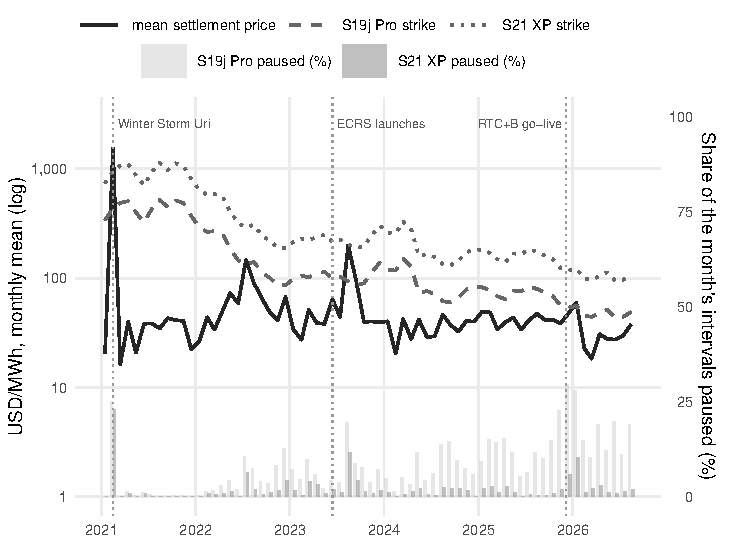
\includegraphics[width=\textwidth]{images/ch9_moving_strike}
  \caption{Five markets, two strikes, and the first months after. Monthly means of the LZ\_WEST real-time settlement point price and of the two machines' strikes, January 2021 to August 2026, on a log scale; the bars are the share of each month's quarter-hours the lagged rule paused each fleet. In 2021 the strikes floated far above every price but Uri's; by 2025 the S19j~Pro's averaged \$72 against a mean price of \$42, close enough that the fleet paused 14~percent of the year; in the eight months of 2026 under RTC+B it paused 17~percent. Strike = hashprice $\times$ 41,667 $\div$ J/TH, at 29.5~J/TH (S19j~Pro) and 13.5~J/TH (S21~XP), on the spliced daily hashprice.} % fig-src: analysis/figures/fig_ch9_moving_strike.R, computed from analysis/data/ercot_rtm15_spp_loadzones_2021on.csv.gz and hashprice_daily_2021on.csv (paused share by year: S19j Pro 2.4% / 4.9% / 7.0% / 7.3% / 13.8% / 16.7% (2026 ytd); S21 XP 2.1% / 1.6% / 2.7% / 1.2% / 1.7% / 2.7%); 2025: mean price $42, S19j strike $72 (the same console); until 2026-10-04 the caption said the S19j Pro's strike "cut through the middle of the price band" in 2025: the figure draws no band, and at $72 against $42 the strike was crossed in 14% of quarter-hours, the upper tail
  \label{fig:stack-moving-strike}
\end{figure}

Figure~\ref{fig:stack-moving-strike} shows the two strikes descending from far above the price in 2021 toward it by 2025, and the pause share rising with them: the S19j~Pro fleet paused 2~percent of quarter-hours in 2021 and 14~percent in 2025, about 1,200 hours, while the S21~XP fleet never paused more than 3~percent in any year. % src: fig_ch9_moving_strike.R console (paused share by year); ch9_flexibility_stack.R Layer 1 (S19j Pro 2025: 1,212 h paused; S21 XP 146 h); 2025: mean price $42, S19j strike $72, S21 strike $157 (fig_ch9_moving_strike.R console); until 2026-10-04 this line had both strikes descending "into its middle", the middle of a price band, by 2025: the figure draws no band, and the S19j Pro's strike was crossed in 14% of 2025's quarter-hours, the S21 XP's in 2%
The figure runs eight months past the ledger, into the first year under RTC+B, and the trend does not bend: hashprice took the S19j~Pro's strike to about \$48 against a mean price of \$32, and the fleet paused 17~percent of quarter-hours, the S21~XP 3~percent. Whether the new market changed the value of those pauses is Chapter~10's question; the ledger stops at the end of 2025 because the reserve side of it changed shape in December. % src: fig_ch9_moving_strike.R console, 2026 (8 months): mean price $32, strikes $48 / $104, paused 16.7% / 2.7%
This is Chapter~4's operating leverage arriving at fleet scale. The old machine, with the thin margin, is the one that keeps crossing its strike, so its strike is worth more per megawatt in every year, 1.1 times the S21~XP's in 2021 and 2.9 times in 2025. It still earns far less: per megawatt, the S21~XP's margin was 2.3 times the S19j~Pro's in 2021 and 3.4 times in 2025, and only price spikes ever cross the S21~XP's strike. % src: ch9_flexibility_stack.R console, Layer 2 (per MW-yr: 950,401 / 854,511 = 1.11 in 2021; 45,983 / 15,938 = 2.89 in 2025); margins per MW of stock draw, ch9_flexibility_stack.R console, Layer 1, real-time index, "flex" column (annual profit, $ millions): S19j Pro 106.94 / 30.68 MW = $3.49M and S21 XP 289.06 / 36.45 MW = $7.93M in 2021 (2.28x), 9.35 / 30.68 = $0.305M and 37.16 / 36.45 = $1.019M in 2025 (3.35x); until 2026-10-04 this line said the old machine "earns more per megawatt" (it is the strike, the value of pausing, that is larger) and put the S21 XP's crossings in "the left tail of the price distribution" (the left end of chapter 6's price duration curve, the right tail of a distribution)
It also settles a question of control: the two fleets must pause on their own strikes, not on a blended site strike. The site-wide breakeven is the strike at the site's power-weighted efficiency, total watts over total terahash, which is 17.95~J/TH and not the mean of 29.5 and 13.5, and a loop that used it would pause the S21~XP when only the S19j~Pro should stop and run the S19j~Pro when it should already be dark. % src: 10,000 x 3,068 W + 10,000 x 3,645 W = 67.13 MW over 10,000 x 104 + 10,000 x 270 TH/s = 3.74 EH/s -> 17.95 J/TH

The engine behind these numbers pauses and resumes without friction; Chapter~5's loop does not, and the cost of its three rules is now measured rather than assumed. The thirty-minute hold with its price deadband, the integral backstop, and the minimum runtimes and daily cycle budget of Section~\ref{sec:threerules} cost the two 2025 fleets, each run alone at the 74.10~MW full-headroom connection, 0.15~percent of their frictionless mining margin before grid charges, about \$81,000 on \$54~million. In exchange they cut the S19j~Pro fleet's stops from 547 to 175 a year and the S21~XP's from 104 to 59. % src: analysis/checks/ch9_control_friction.R console (2025 only; fleets simulated independently at 74.10 MW; mining profit before charges: $53,741,258 frictionless vs $53,660,694 with chapter 5's rules, -$80,564 = 0.15%; stops 547 -> 175 and 104 -> 59, on the S21 XP's 2,774 W floor (-$78,767 and 103 -> 58 on its 2,200 W best point, the floor until 2026-09-26); 35,040 intervals, the full calendar; constants from analysis/ch5-backtest/papo_sim.py)
The price-only figures of this chapter are therefore a ceiling that sits about 1.3~percent, measured on 2025, above the gains a site running the loop would have made, the same \$81,000 taken as a share of the gains rather than of the margin, before any target move is charged; the reserve path holds the fleet on the meter and carries no such gap. That is the second caveat the chapter carries throughout, and it is a small one. % src: analysis/checks/ch9_control_friction.R console, 2025: neither run charges anything for a power target move, at 18.6 and 1.6 target moves a day frictionless against 14.8 and 1.0 under chapter 5's rules (S19j Pro, S21 XP); the per-move cost is chapter-5.tex, Three Facts (braiinsacademyautotuning, braiinsacademydps); the never-pausing site obeys no rules, so the whole $80,564 comes out of what the strike and the power target added: ch9_flexibility_stack.R console, Layer 4 connection table, 2025, 74.1 MW site total $6,075,066 over never pausing (the friction run's connection; CONNECTION NET 2025 the same), 80,564 / 6,075,066 = 1.3% (by fleet 35,847 / 2,054,163 = 1.7% for the S19j Pro and 44,718 / 4,020,903 = 1.1% for the S21 XP, ch9_control_friction.R per-fleet profit lines); until 2026-10-04 this line put the ceiling "about 0.15 percent" above, the share of the whole mining margin (line above), not of the gains the chapter prints

\section{Layer Two: The Power Target}
\label{sec:stack-power-target}

Chapter~5 opened the single operating point into a curve; this layer prices running the whole site on it. The lever is the power target: the firmware holds a machine at any power level in a range, overclocking above stock or underclocking below it, and retunes every chip or loads a saved profile, so the loop can choose in each quarter-hour not only whether to run but how hard. On the measured curves the S19j~Pro runs from 23.8~J/TH at 1,200~W to 28.5 at its 3,068~W stock point and up to a 3,420~W ceiling, and the S21~XP from 12.7~J/TH at its 2,774~W floor, Braiins~OS's default minimum, through its most efficient power target, 12.4 at 3,200~W, to 12.8 at stock and up to 3,990~W. In every quarter-hour the loop picks, from the same lagged information as the strike, the power target that maximizes profit for each fleet, with the connection shared between them. % src: analysis/checks/ch9_tuning.R header (floors, stock points, ceilings; PSU x 0.95 rule); the S21 XP's floor is ch9_floor, Braiins OS's default minimum power target (braiinsacademytechres, as chapter-5.tex prints it), 12.688 J/TH at 2,774 W interpolated between 12.623 at 2,600 W and 12.698 at 2,800 W (ch9_curve jth_floor; ch9_flexibility_stack.R console, Layer 4: floor 2774 W = 12.69 J/TH); most efficient power target 12.443 J/TH at 3,200 W, the measured point (ch9_curve jth_best and p_best; ch9_flexibility_stack.R console, Layer 4: best 12.44 J/TH at 3200 W); analysis/data/miner_efficiency_telemetry_2026q2.csv (23.831 J/TH at 1,200 W; 28.48 J/TH at 3,068 W; 12.81 at 3,645 W); a saved profile or a fresh tuning run, as chapter-5.tex, Three Facts (braiinsacademyautotuning)
Two provenance notes belong here, both from Chapter~5. The curves are averages of fleet operating data, from machines running autotuning firmware, which is why they beat the nameplate at stock power: 28.5 against 29.5~J/TH for the S19j~Pro, 12.8 against 13.5 for the S21~XP. A fleet on stock firmware has one operating point, not a curve, and sits at the nameplate; the layer priced here is available only to a fleet that has changed its firmware, and that gap at stock, 1.0 and 0.7~J/TH, is part of what it buys. % src: chapter 5 sec "One Point Becomes a Curve" (fleet averages from Braiins OS telemetry, 2026-Q2, analysis/data/miner_efficiency_telemetry_2026q2.csv; "at stock power the autotuned fleet average actually beats the nameplate"); chapter 4 nameplate 29.5 and 13.5 J/TH (bitmain2021s19jpro, bitmain2024s21xp)
Moving the target also widens the range in which the site runs at all, because the pause threshold moves from the breakeven at stock to the breakeven at the most efficient power target in the loop's range: 20~percent higher for the S19j~Pro, only 3~percent for the S21~XP, whose curve is too flat to make underclocking worth anything, exactly the asymmetry Chapter~5 described. % src: 29.5 / 23.83 - 1 = +24% at nameplate, 28.5 / 23.83 - 1 = +20% at the curve's stock point; 12.8 / 12.44 - 1 = +3% (12.81 / 12.443 - 1 = +2.9%), the S21 XP's best J/TH in range at 3,200 W, above its 2,774 W floor (12.397 at its 2,200 W best point, the floor until 2026-09-26); analysis/checks/ch9_tuning.R ch9_curve jth_best 23.831 and 12.443 (ch9_flexibility_stack.R console, Layer 4: best 23.83 J/TH at 1200 W and 12.44 J/TH at 3200 W)
Braiins~OS is paid for in hashrate: a \glossaryterm{development-fee}{development fee}, or devfee, of 2.5~percent on these two machines, collected by assigning that share of each machine's hashrate to Braiins Pool, the company's mining pool \autocite{braiinsoslicense,braiinsosfirmware}. The ledger omits it: at that rate it would have taken about \$1.8~million of the site's 2025 mining revenue, beside the \$3.1~million the power target added that year (below); it falls on all of a machine's hashing, not this layer alone. % src: braiinsoslicense sec. 5.2 ("As license fees You will provide to Braiins a portion of the processing power generated by any and all cryptocurrency mining devices on which the Software is used"), 5.4 (the percentage shown on the Website or in the Fee List; "If the percentage is visibly indicated neither on the Website, nor in the Fee List issued by Braiins, nor was the percentage otherwise agreed upon, the percentage shall be 2,5 %"), 5.5 (at all times the device's processing power is used), 5.6 (the software automatically assigns that processing power to operations "designated and sent to You by Braiins"); braiinsosfirmware (pricing panel "2.5% dev fee"; FAQ: "a 2-2.5% dev fee (depending on the hardware model) by directing that percentage of your hashing power to our pool"); the rate: no public fee list by model was found on braiins.com or on the 85 Braiins OS, Pool and Manager pages of academy.braiins.com/sitemap.xml (2026-09-27), so nothing published gives the S19j Pro or S21 XP less than 2.5%, and the licence default and the website's 2.5% apply; corroborated, not cited in print, by braiins.com/blog/review-of-bmm-100-by-german-mining-community (11.11.2024, a German mining community's review on the Braiins blog, read 2026-09-27: "After checking with Braiins, this applies to current devices", and "an S9 is operated with a DevFee of 2% and an S19 and newer with a DevFee of 2.5%"), so the 2% of the FAQ's range is the S9's; Braiins Pool as the fee's destination per the author (2026-09-27), the FAQ's "our pool"; no Academy page found that names it; the fee: analysis/checks/ch9_optimal_stack.R console, 2025 FIRMWARE FEE line (both round to about $1.8M: planned site's mining revenue before energy $71,145,385, never pausing $72,419,582; at 2.5% $1,778,635 and $1,810,490, $26,495 and $26,970 per MW-yr; the power target's increment $3,112,106, the tuning_gain of analysis/data/ch9_optimal_stack.csv); the pool fee is a separate charge and is not priced here

The accounting matters, because this is the layer most easily counted twice. Measured against stock power that never pauses, its gain already contains the strike, since the curve's cheapest point is ``off''. The ledger therefore books the power target as the increment over a site that already pauses but never leaves stock power. On that basis the 2025 site earned \$1.9~million from the strike and a further \$3.1~million from the power target: the target was worth more than the strike. Across the five years the increment ran \$18.9~million, \$7.5~million, \$4.4~million, \$3.9~million and \$3.1~million, against strike gains of \$59.8~million, \$6.6~million, \$12.7~million, \$2.2~million and \$1.9~million. % src: analysis/checks/ch9_optimal_stack.R console, L1 and L2 lines (strike_gain and tuning_gain columns of analysis/data/ch9_optimal_stack.csv)
The target beat the strike in 2022, 2024 and 2025 and lost to it in 2021 and 2023. % src: the line above, tuning_gain against strike_gain of analysis/data/ch9_optimal_stack.csv: target ahead in 2022 ($7.50M vs $6.61M), 2024 ($3.95M vs $2.19M) and 2025 ($3.11M vs $1.89M), behind in 2021 ($18.90M vs $59.79M) and 2023 ($4.41M vs $12.73M)

The connection binds. At full tilt the fleet would draw 74.10~MW against a 67.13~MW connection, so a cap on the site behaves like a surcharge on power: the S21~XP pins at its ceiling and the S19j~Pro is held below stock to make room, and under a tight connection moving the targets is largely a reallocation between the fleets rather than a windfall. The companion repository prices the difference: raising the connection from 67.13 to 74.10~MW would have added about \$0.9~million to the 2025 margin after power and grid charges, and every extra megawatt of connection is still, at the machines, under the 75~MW line. % src: ch9_flexibility_stack.R console, Layer 4 connection table, 2025: 67.1 MW $4,999,407 vs 74.1 MW $6,075,066 (gains vs never-pause; +$1,075,659); before grid charges like the strike and power target gains it sums (2025 strike_gain $1,887,301 + tuning_gain $3,112,106 = $4,999,407, analysis/data/ch9_optimal_stack.csv), so the larger connection's grid charges would come off it, among them the distribution billed on a monthly peak up to 7.20 MW higher: (74.10 - 66.90) x 1,000 x $0.339183 x 12 = $29,305 a year at most (analysis/checks/oncor_distribution.R; 66.90 MW the tuned site's monthly peak, ch9_optimal_stack.R console, 2025 DISTRIBUTION PEAKS line); "before grid charges" added 2026-10-03, when the ledgers began billing distribution on each month's peak; printed as "about $0.9 million after power and grid charges" since 2026-10-03 from ch9_flexibility_stack.R console "CONNECTION NET 2025": 74.10 vs 67.13 MW gain +$1,075,659, energy-keyed charges (losses, ancillary, uplift on the extra megawatt-hours, chapter 6 ledger rates) +$97,315, distribution on the higher monthly peaks +$29,305, net +$949,039; no transmission charge on either connection, since the planned site plays the summer window in 2025; "$1.1 million before grid charges" earlier on 2026-10-03
A site built to this design brief would size its connection just under the line, counting every load at its meter: near 74~MW if nothing but machines drew from it, full headroom for the efficient machine, but about 68~MW of machines once Chapter~1's tenth more for cooling and transformer losses is counted, close to the ledger's own connection. % src: 75 - 74.10 = 0.90 MW left under the line if the machines ran flat out, against 7.41 MW of cooling and losses (10% of 74.10 MW); 75 / 1.10 = 68.18 MW of machines at most (chapter-1.tex:116, CBECI2026 PUE 1.10); the ledger's connection is 67.13 MW, 73.84 MW at the meter; until 2026-09-27 this line sized the connection near 74 MW with 0.9 MW of margin, the machines alone (PER-3 review round)
The power target is a firmware benefit, not a grid benefit: a site behind a fence with the same firmware gets it too, so the fenced site of Section~\ref{sec:stack-fence} moves its target as well. % src: until 2026-10-04 this line said "when Section 9.8 compares the two sites the target is counted on both sides": the fence moves its target in every year (tab:stack-fence caption, power targets free on both sides), but the grid sites it is held against run at stock power wherever they hold no target: the never-pausing site in every year, the planned site in 2022 and 2024 and the hindsight ceiling in 2021 and 2023, the reserve years (ch9_optimal_stack.R, the reserve path "always on at stock"; tab:stack-ledger italics)

\section{Layer Three: Reserves, or the Strike}
\label{sec:stack-reserves}

Chapter~7's catch (Section~\ref{sec:as-catch}), restated as arithmetic: a megawatt that holds a reserve award must stay on the meter through every hour of the award, so before RTC+B it cannot also take the strike. The layer is an either/or per megawatt-year: the standing revenue of the best product, the ceiling Chapter~7 defined as one megawatt holding the award through every hour at the day-ahead clearing price, against the strike gain the same megawatt forfeits. Table~\ref{tab:stack-markets} carries the verdicts. Per megawatt of S19j~Pro the reserve won in four years of five, by a mile in 2021, when RRS paid \$2.7~million per megawatt-year against a strike worth \$950,000, and narrowly in 2024, \$72,000 against \$46,000. In 2025 the answer flipped: the best product paid \$27,000 and the strike \$46,000. % src: ch9_flexibility_stack.R console, Layer 2 table (2021 RRS 2,735,205 vs 950,401; 2022 NonSpin 196,973 vs 120,344; 2023 ECRS 286,136 vs 217,602; 2024 ECRS 72,308 vs 45,918; 2025 NonSpin 26,699 vs 45,983)
The 61-fold compression of Chapter~7 turned the sign, and the batteries of Chapter~6 did the compressing.

The site is not one megawatt, and the joint engine can send one fleet into reserves while the other runs the strike and the power target. Weighed that way, the reserve path wins less often than the per-megawatt table suggests. In 2022 Non-Spin beat the strike per megawatt but not the strike plus the power target, and in 2024 the same held for ECRS; in 2025 no combination with reserves came within \$2.5~million of the price-only stack, even though per megawatt the S21~XP's own strike, at \$16,000, was worth less than a Non-Spin award. % src: analysis/checks/ch9_optimal_stack.R console, L4 rows, 4CP on (2022: both on NonSpin $146.92M vs the price-only stack $148.04M; 2024: both on ECRS $71.15M vs $72.59M; 2025: S21 XP on NonSpin $47.20M vs $49.77M, $2.57M short); per MW, ch9_flexibility_stack.R Layer 2, 2025 "strike S21" $15,938 against NonSpin $26,699 (printed $17,000, the clipped $17,010, until 2026-09-27)
The award holds the machine at stock power, and the strike and power-target gains it forfeits were worth more than the award in those three years. % src: analysis/checks/ch9_optimal_stack.R console, L1 and L2 lines and the L4 "both fleets on" rows: strike + power target 2022 $6,605,259 + $7,501,880 = $14.11M vs NonSpin $11,982,715; 2024 $2,192,769 + $3,948,617 = $6.14M vs ECRS $4,751,000; 2025 $1,887,301 + $3,112,106 = $5.00M vs NonSpin $1,781,137; until 2026-10-04 this line said "the power-target gain it forfeits is worth more than the award", false at site scale in 2022 ($7.50M vs $11.98M) and 2024 ($3.95M vs $4.75M)
Only in 2021 and 2023 did reserves win, for both fleets, and only with the year's outcomes in hand: RRS through the storm, and ECRS through its first, artificially scarce year.

Standing revenue assumes an award in every hour at the clearing price, with no QSE fee, no deployment cost and no failed-performance event, Chapter~7's convention, and 91~percent of 2021's RRS figure fell in the seven days of Uri. % src: ch9_optimal_stack.R console, "2021 RESERVES" line ($2,485,794 of $2,734,995 per MW-yr in Feb 14-20, the ledger's 2021 from January 2; the stack script's calendar year gives $2,735,205, as tab:stack-markets prints); analysis/data/ercot_dam_as_mcpc.csv.gz
The ledger books the reserve path conservatively, with the fleet buying every interval at the settlement price even in the storm hours when a deployed load resource would have been off and paid, so on that convention the 2021 figure is a floor. On every other count, no QSE fee or credit support, no deployment cost, no failed hour and a full-site award that Chapter~7's caps would not allow on RRS (Section~\ref{sec:clr}), it is a ceiling. And which fleets to commit, and to which product, is a choice the site must make before the year starts, so the ledger makes it twice. With the year's own outcomes in hand it is the hindsight ceiling of Section~\ref{sec:stack-sum}. Made as an operator could have made it, in January on the previous year's ledger, it commits both fleets to RRS in 2022, the year after Uri, and to ECRS in 2024, the year after ECRS's launch, and runs the price-only stack in the other three years. It said to sell twice and lost both times: \$2.4~million in 2022 and \$1.4~million in 2024 against never selling reserves at all. % src: ch9_optimal_stack.R console, PLANNED and ALTERNATIVE PLANS lines (2022 planned both on RRS $11,940,729 vs never sell reserves $14,352,955; 2024 both on ECRS $5,241,288 vs $6,681,877), and the five-year line "where the planned reserve choice differs from never selling reserves: 2022 -2.41M; 2024 -1.44M" (2024 was -1.45M, printed $1.5 million, until 2026-10-03, when the ledgers booked distribution at $0.50 per MWh consumed); award quantity: every reserve row books the whole allocated fleet awarded in every hour (ch9_optimal_stack.R score(), asrev = as_mw x rate), while chapter 7 sec:clr prints the RRS limits (relay loads prorated, 1,480 of 7,568 qualified MW supplied in 2025; a new CLR's RRS at 20% of its maximum consumption, about 13 MW for this site)
A per-fleet version of that rule did worse. It compared, fleet by fleet, a megawatt of standing revenue with that fleet's own strike-and-power-target gain per megawatt; fed each year's own numbers it picked the year's best choice in only two years of five, because one fleet's power-target gain depends on the other fleet making room under the connection, and a per-megawatt view leaves out the window and the charges. Fed the previous year's numbers, it would have earned \$11~million less over the five years than the whole-site rule the ledger runs. % src: ch9_optimal_stack.R console, "CHOICE RULES FED THIS YEAR'S OWN DATA" lines (old rule equal to the best in 2021 and 2025; $5,134,962 below in 2022, $3,484,726 in 2023, $3,144,123 in 2024); five-year alternatives line (old per-fleet rule on last year's data $112.37M vs planned $123.46M)
Before RTC+B a reserve award was a bet that the year would repeat, and in this ledger the years that paid for reserves did not.

A seller does not offer the summer window, since an award held through a 4CP afternoon would cost the peak, so wherever the window is played the engine removes what the window's hours actually paid at the day-ahead clearing price. That is not the window's 2~percent share of the year's hours: in 2022 and 2023 a summer afternoon was when reserves cost most, and the window's hours carried 10~percent of RRS's standing revenue in 2022 and 21~percent of ECRS's in 2023, against half a percent of RRS's in the storm year and 2~percent or less in 2024 and 2025. % src: ch9_optimal_stack.R console, "WINDOW HOURS' SHARE OF STANDING REVENUE" lines (RRS 0.5% in 2021, 9.9% in 2022; ECRS 21.4% in 2023; 2024 RRS 1.1%, ECRS 2.1%, NonSpin 1.5%; 2025 RRS 0.6%, ECRS 0.8%, NonSpin 0.6%; the window's share of the year's hours 2.0%); hours ending 17 and 18 on June-September weekdays in analysis/data/ercot_dam_as_mcpc.csv.gz; until 2026-10-04 this line said, of no year in particular, that "a summer afternoon is when reserves cost most", which its own lines show only for 2022 and 2023
And from December 2025 the either/or dissolves: under RTC+B a load buys out of its reserve position at the real-time ancillary price and pauses, so the conflict becomes a price. Chapter~8 found that a two-hour buyout on the official 4CP afternoons, priced at day-ahead clearing prices, would have cost under \$160 per megawatt on fourteen of the twenty. % src: chapter 8 sec:fourcp-econ (buyout priced at DAM clearing prices of the 20 official afternoons 2021-2025)
Only partial 2026 data exists, so this chapter states the mechanism and hands the number to Chapter~10.

\section{Layer Four: The Peaks the Price Never Flags}
\label{sec:stack-peaks}

Chapter~8 found that the energy price no longer marks the system peak (Section~\ref{sec:fourcp-factors}). At the scale of this site that finding has a price. The strike alone would have paused the fleet in none of the four official 4CP intervals of 2021, 2024 and 2025, in one of four in 2022, and in 2023 in three of four for the S19j~Pro and two for the S21~XP. % src: ch9_flexibility_stack.R console, Layer 3 coverage lines (S19j Pro 0/4, 1/4, 3/4, 0/4, 0/4; S21 XP 0/4, 1/4, 2/4, 0/4, 0/4)
The peaks must therefore be a layer with its own hours, triggered by demand and the clock rather than by price. The summer window, about 175 hours a year, scored after the fact against the official intervals, caught all four peaks in every year but 2024, when it caught two and the site paid half the charge. % src: ch9_optimal_stack.R console, L3 lines (172-176 h; caught 4/4 except 2024 2/4, TCRF $1,406,407 paid; the misses are Sunday 2024-06-30 and 2024-09-20, whose interval 15:45-16:00 ended as the window opened)

What the window cost depends entirely on the strike. In 2021 it lost \$5.5~million: the site's blended strike, about \$720 at its average 17.95~J/TH, made the margin forgone in 176 hours dwarf a transmission prize of \$2.8~million. That prize is the site's 67.13~MW at Chapter~8's floor of \$41,900 per megawatt-year, held here for every year although the rider ran higher through 2024 and 2025, so the prize and the rule below are understated. From 2022 the window paid, \$1.3~million, \$1.7~million, \$0.4~million and \$1.6~million net of the margin given up. % src: ch9_optimal_stack.R console, L3 lines (net over L2: 2021 -$5,523,656; 2022 +$1,254,678; 2023 +$1,747,178; 2024 +$409,542; 2025 +$1,606,871; exposure 67.13 x $41,901 = $2,812,814; 2023 was +$1,751,830, printed $1.8 million, until 2026-10-03, when the ledgers booked distribution at $0.50 per MWh consumed, which the window's hours appeared to save); 2021's window ran 176 h (2021 L3 line, "176 h off"; fourcp_hours, analysis/data/ch9_optimal_stack.csv), printed 175 until 2026-10-03; the site strike: 2021 WINDOW RULE line, "with the year's mean hashprice ... strike $721" at the site's 17.95 J/TH (the fleets' own $439 and $958, 2021 header line), against a margin forgone of $5,523,656 + $2,812,814 = $8,336,470 over 176 h; until 2026-10-04 this line said "a $440 strike", the S19j Pro's alone, though the window empties both fleets
The wider rule Chapter~8 also tested, every day from 2 to 6~p.m., loses money in all five years at this site. % src: ch9_optimal_stack.R console, "L3 alt 4CP rule A" lines, the ledger's tuned site, charges and scoring, 488 h, 4 of 4 peaks caught each year: net over L2 -$20,118,868 / -$1,526,435 / -$232,737 / -$118,650 / -$661,853 (the calculator, rule A, the same); on the stack script's nameplate, stock-power basis it lost in four of five (ch9_flexibility_stack.R Layer 3, rule A: +$126,890 in 2024), the basis this line printed until 2026-09-27; lag sensitivity (CH9_LAG_Q=2, a full quarter-hour late): 2023's L3 alt 4CP rule A line turns from -$232,737 to +$21,073, the only year to flip; at the measured delay, about a third of a quarter-hour, a linear reading keeps it negative (about -$148,000), so the sentence holds, with that margin

The operator's rule falls out of the arithmetic and needs no forecast. The annual window decision compares the whole site's forgone margin with its transmission saving; quarter-hour pauses need a separate strike for each machine model. The prize is about \$41,900 per megawatt and the window about 175 hours, so the window pays as long as the margin the site forgoes per megawatt-hour of window time is under about \$240. The margin that matters is the site's, at the strike of its power-weighted 17.95~J/TH, and it must be a margin the site can know on June~1: the strike on yesterday's hashprice, as step~1 of Section~\ref{sec:stack-rule} computes it, against last summer's window price, not this summer's. On those terms the rule gives the same call as hindsight in three of the four years it can be applied. In 2023 and 2024 the previous summer's window had priced above the strike, at \$197 and \$331: play. In 2025 a strike of \$121 against \$33 leaves \$87: play. % src: ch9_optimal_stack.R console, WINDOW RULE lines (threshold $41,901 / 172-176 h = $238-$244; site strike on June 1 = the previous day's hashprice x 41,666.7 / 17.95: $523 / $308 / $168 / $126 / $121; last summer's window means $60.32, $196.58, $331.36, $33.49; this summer's 2025 $35.32)
In 2022 it says skip: a strike of \$308 on the last day of May against 2021's window price of \$60 leaves \$248, just over the \$238 threshold, and that window went on to pay \$1.3~million. The skip is narrow. It would flip back to play if the transmission prize were 4~percent above the \$41,900 floor this chapter holds constant, and on the year's mean hashprice, which no one knows in June, the strike would have been \$283 and the call play. % src: ch9_optimal_stack.R console, 2022 WINDOW RULE line (margin $248 vs $238: skip; flips if the prize were 4.0% higher; year's mean hashprice: strike $283, margin $223, play; the window paid $1,254,678 net); until 2026-10-04 this line said "the $60 the window had cost in 2021": the $60 is last summer's window price, $60.32, while the 2021 window's cost was the $5.5 million loss above
Only 2021 has no prior summer in the data. On June~1 its strike was \$523, so the window would have paid only if its hours averaged above \$285; the planned site of Section~\ref{sec:stack-sum} does not play a window it has no evidence for, and hindsight agrees: the 2021 window lost \$5.5~million. % src: ch9_optimal_stack.R console, 2021 WINDOW RULE line (strike $523 on the previous day's hashprice $0.2253; pays only above $285; the window lost $5,523,656 net)
Chapter~8's 66-hour hindsight haystack roughly bounds what any better method could add; none appears in this book. % src: analysis/figures/fig_ch8_4cp_window.R median 66.25 h within 2% of the reconstructed monthly peaks

Two proposals would end the layer, and both are in Chapter~8. For a new large load, and for the added megawatts of the expansions the rule covers, the minimum billing demand makes transmission a fixed cost; this site is designed to stay under the line. For everyone else the 12CP reform would turn four peaks worth \$41,900 per megawatt into twelve worth about \$3,500 each, spread over two seasons. % src: chapter 8 sec:twelvecp ($3,492 per peak; the minimum reaches only loads covered by the adopted 25.194: new sites of 75 MW or more and, for an expansion, only the incremental load of one that first takes a site to 75 MW or adds 75 MW or more to a site already past it, puct2026order58481 25.194(b)(1)(A)-(C) and (b)(2)); both still proposals on 2026-09-26: puct2026prop58000, with no adoption order among the 67 filings in PUCT Project 58000, the last filed August 11, 2026, and texas2025sb6 sec. 6(c) requires amended rules by December 31, 2026, not 12CP
A reader above the line can take the price-only stack of this ledger by the megawatt, since it scales with the fleet and the connection; under the minimum as proposed, a new site, or the added megawatts of an expansion, would lose the window column of Table~\ref{tab:stack-ledger}, which leaves \$5.2~million of 2025's \$6.8~million, and Chapter~10 gives that figure at lower hashprices (Table~\ref{tab:outlook-sensitivity}). Whether the minimum also reaches a load already running is unresolved as this book goes to press. % src: scale: analysis/checks/ch9_tuning.R ch9_tune_site (profit linear in units; connection test p19 x units19 + p21 x units21 <= cap_w) and ch9_optimal_stack.R score() (adders, TCRF and distribution's per-kW charge on the monthly peak linear in MW; distribution's $580.43 a month of customer and metering charges is fixed per meter and cancels in every flexibility figure, since both sites pay it; analysis/checks/oncor_distribution.R), so the price-only stack scales with fleet and connection together; the reserve rows only as a price-taker; analysis/data/ch9_optimal_stack.csv 2025 (plan_flex $6,774,783 - fourcp_net $1,606,871 = $5,167,912, the flex_nowin_value of the 100% row of analysis/data/ch10_hashprice_sensitivity.csv); the minimum's reach: puct2026order58481 25.194(b)(1)-(2), as chapter 8 sec:twelvecp prints; a load already energized: chapter-8.tex:170 (outside the minimum as proposed, contested in the Project 58000 comments: TBC Item 41, American Bitcoin Item 14, OPUC Item 63), and no adoption order among the 67 filings of PUCT Project 58000 on 2026-09-26 (this line's neighbour above); the window's share of flexibility is 23.7% in 2025 and 9.1% and 7.8% in 2023 and 2024, so no single share is printed
The figures of this section are the record of the game as it was played from 2021 to 2025, and perhaps of the last summers in which it can be played this way.

The emergency and utility programs of Section~\ref{sec:programs} get one paragraph, because they collide with this layer. ERS cleared at \$4.36 per megawatt per hour on average in 2025 and at \$18.69 in its summer-afternoon block, the summer term's best-paid one, which contains 29 of the 32 official 4CP intervals of 2018 to 2025; an ERS commitment is a commitment to be on the meter at exactly the moments this layer wants the site dark, so a site that keeps its afternoons free can sell only the mornings, weekends and leftover hours. The wires utilities' own load-management programs are closed to a for-profit site at transmission voltage. Aggregator fees are private and stay unprinted. The ledger leaves the programs out; on Chapter~8's 2025 prices those other blocks would have paid the S21~XP fleet about \$0.65~million, a tenth of that year's flexibility. % src: chapter 8 sec:programs (ERS 2025 average clearing price $4.36/MW/h, potomac2026somercot p. 32; June-September 2025 Time Period 4 $18.69, ercotersproc2025 via analysis/checks/ch8_ers_blocks.R; Time Period 4 vs the official intervals, 29 of 32 in analysis/checks/ch8_4cp_peaks.R console; Oncor's exclusion of for-profit transmission-voltage load); the bound: analysis/checks/ch8_ers_blocks.R console, Time Periods 1, 6, 7 and 8 of the four terms $17,948 per MW x 36.45 MW = $654,205, against the planned site's 2025 flexibility $6,774,783 (analysis/data/ch9_optimal_stack.csv plan_flex) = 9.7%; the S19j Pro's strike crosses more than 5% of those blocks' hours, the S21 XP's 4.2% at most (the same console, as chapter 8 prints); $18.69 is the highest of the June-September 2025 term's eight Time Periods (Time Period 5 next at $18.08), and the program year's dearest block was December-March Time Period 1, weekdays HE 06-09, at $26.87 (analysis/checks/ch8_ers_blocks.R console, as chapter-8.tex sec:programs notes); until 2026-10-04 this line called the summer-afternoon block "the best-paid one"

\section{The Sum That Isn't}
\label{sec:stack-sum}

One rule sits under everything above: a megawatt does one thing in one quarter-hour. Any two layers that want the same megawatt in the same interval cannot both be booked, and the ledger has five such collisions and two deductions that touch every line. Reserves against the strike is an annual either/or that removes the smaller line. The window against the strike is margin spent on hours the price never flagged. Reserves against the window is standing revenue forgone in the window. The power target against the strike is counted only as an increment. The power target against the connection is the cap that turns an overclock into a reallocation. Friction is the 0.15~percent of mining margin Chapter~5's rules cost. And information is the gap between the lagged loop and its perfect-foresight twin on every line, and one level up, the gap between the annual switches set in advance and the same switches set in hindsight.

Those two switches are where hindsight would pay most. Which fleets hold reserve awards, and in which product, has to be settled for the year; whether to play the summer window has to be settled by June. So the ledger prints the site twice, the way Chapter~5 grades the loop against its oracle. The \glossaryterm{planned-site}{planned site} sets both switches with what was known at the time. In January it commits to the reserve allocation and product that won the previous year's ledger, and in 2021, the first year in the companion repository's data, with no history, it sells no reserves; on June~1 it calls the window by the rule of Section~\ref{sec:stack-peaks}. The \glossaryterm{hindsight-ceiling}{hindsight ceiling} is the best annual choice in hindsight: every allocation, every product and the window on or off, scored on the year's own outcomes. It needs the year's prices before the year starts, and in 2021 it needs to know in January that Uri is coming. The planned site is the headline, and the ceiling is printed beside it and never called a strategy. % src: analysis/checks/ch9_optimal_stack.R header (TWO ANNUAL CHOICES) and console PLANNED and HINDSIGHT CEILING lines
Last year's winner is the rule because it is the one an operator reaches for and it asks the ledger for nothing the operator did not hold in January. Figure~\ref{fig:stack-shape} and Table~\ref{tab:stack-ledger} put the whole ledger on one engine, and the paragraphs after them report the other rules an operator might have chosen.

\begin{figure}[htbp]
  \centering
  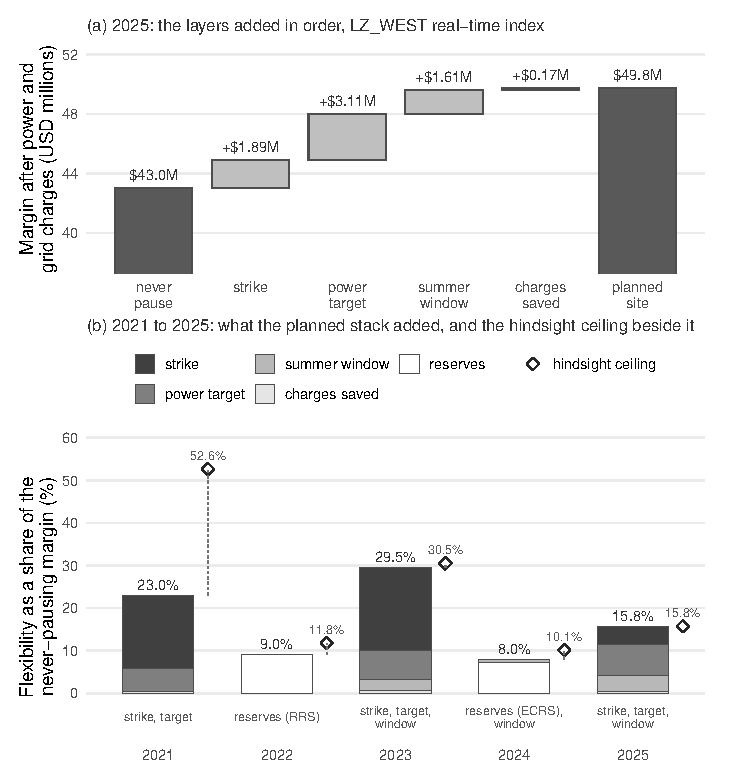
\includegraphics[width=\textwidth]{images/ch9_stack}
  \caption{What the stack was worth, as margin after power and grid charges: mining and reserve revenue, no pool or firmware fee taken out, less the energy and the grid charges. The retail adder, the machines, their depreciation, those fees, site operation, staff and debt are outside the ledger. (a)~2025 as a waterfall: the never-pausing site's margin, then each layer added in the order the chapter stacks them, to the planned site, which in 2025 is also the hindsight ceiling; ``charges saved'' is the losses, ancillary and uplift the paused and underclocked megawatt-hours avoided, plus under \$1,000 of distribution from a lower monthly peak. (b)~2021 to 2025: the value of flexibility to the planned site as a share of the never-pausing site's margin, decomposed along the path it ran. In 2022 and 2024 it had committed both fleets to a reserve award on the previous year's winner, and the reserves segment is Chapter~7's standing revenue. The diamond beside each bar is the hindsight ceiling; in 2021 its 52.6~percent is the RRS award through Uri. The reference site is 67.13~MW (10,000 S19j~Pro and 10,000 S21~XP) at LZ\_WEST, on 15-minute settlement prices and the spliced daily hashprice, with lagged decisions. The planned site commits its reserves each January on the previous year's winner (none in 2021) and calls the summer window on June~1; while it holds reserves, the fleet stays on the meter.} % fig-src: analysis/figures/fig_ch9_stack.R on analysis/data/ch9_optimal_stack.csv (planned 23.0 / 9.0 / 29.5 / 8.0 / 15.8%; hindsight 52.6 / 11.8 / 30.5 / 10.1 / 15.8%, 52.7 and 10.2 until 2026-10-03, when the ledgers booked distribution at $0.50 per MWh consumed); charges saved, 2025: $0.17M (fig_ch9_stack.R console 0.1685) = plan_flex $6,774,783 less strike_gain $1,887,301, tuning_gain $3,112,106 and fourcp_net $1,606,871; its distribution part is ch9_optimal_stack.R console, 2025 DISTRIBUTION and DISTRIBUTION PEAKS lines: never pausing $280,197 billed on 67.13 MW every month, planned $279,261 on monthly peaks of 66.90 MW, 0.23 MW x 1,000 x $0.339183 x 12 = $936; the tuned site's highest quarter-hour is 66.90 MW (S19j Pro 2,700 W + S21 XP 3,990 W a pair) and the never-pausing site is billed on its 67.13 MW nameplate draw, the draw its other charges are booked on, though its energy is priced at the curves' stock points, 67.00 MW, so 0.13 of the 0.23 MW is that booking and 0.10 MW the tuned site's own lower peak; the bill is chapter 6's (analysis/checks/oncor_distribution.R: $0.331004 + $0.008179 per billing kW-month on the month's highest quarter-hour, an 80% ratchet that binds in no month, DISTRIBUTION CHECK line, and $580.43 a month at the one site meter); until 2026-10-03, when the ledgers booked distribution at $0.50 per MWh consumed, the caption counted distribution among the charges a paused megawatt-hour never incurred; the margin basis (EXEC-020): analysis/checks/ch9_optimal_stack.R, total = mining - adders - dist - tcrf + asrev, mining = hashprice x terahash (analysis/data/hashprice_daily_2021on.csv usd_th_day_spliced, no fee deducted) less energy at the settlement price, adders, dist and tcrf the grid charges of chapter 6's tab:btm-ledger (dist since 2026-10-03, when it left the adders); no retail adder (private and excluded, analysis/checks/ch6_btm_ledger.R header), machine, depreciation, fee, site operation, staff or debt line anywhere in the ledger, as chapter-4.tex:77's breakeven ignores the machine, hosting, cooling and staff; the firmware fee, Braiins OS's 2.5% devfee, is priced beside the power target in sec:stack-power-target (ch9_optimal_stack.R FIRMWARE FEE line), not in the ledger; printed as "under $1,000" since 2026-10-03 because $529 of the $936 is the never-pausing site billed on its 67.13 MW nameplate against energy priced at 67.00 MW, and only $407 the tuned site's own lower peak
  \label{fig:stack-shape}
\end{figure}

\begin{table}[tb]
  \centering
  \scriptsize
  \setlength{\tabcolsep}{1.8pt}
  \begin{tabular}{lrrrrrrrr}
    \hline
    \textbf{Year} & \textbf{Never} & \textbf{Strike} & \textbf{Target} & \textbf{Window} & \textbf{Planned} & \textbf{Flexibility} & \textbf{Hindsight} & \textbf{Interf.} \\
     & pause & & & net & site & \$M (\%) & \$M (\%) & \\
    \hline
    2021 & 348.72 & 59.79 & 18.90 & \emph{$-$5.52} & 428.93 & 80.20 (23.0) & 183.60 (52.6) & $-$6.82 \\
    2022 & 132.43 & \emph{6.61} & \emph{7.50} & \emph{1.25} & 144.37 & 11.94 (9.0) & 15.61 (11.8) & $-$1.31 \\
    2023 & 65.49 & 12.73 & 4.41 & 1.75 & 84.78 & 19.29 (29.5) & 19.97 (30.5) & $-$0.67 \\
    2024 & 65.91 & \emph{2.19} & \emph{3.95} & 0.41 & 71.15 & 5.24 (8.0) & 6.68 (10.1) & $-$2.27 \\
    2025 & 43.00 & 1.89 & 3.11 & 1.61 & 49.77 & 6.77 (15.8) & 6.77 (15.8) & $-$1.04 \\
    \hline
    Total & & & & & & 123.46 & 232.63 & \\
    \hline
  \end{tabular}
  \caption{The ledger, in millions of dollars per year, LZ\_WEST real-time index, one engine. ``Never pause'' is the site at stock power in every interval. Strike and power target are margin before grid charges; never pause and planned site are after them, the full transmission charge included. Strike, power target and window are the increments of the price-only stack in that order; italics mark a layer the planned site did not run that year. The planned site sets the two annual switches in advance: reserves in January on the previous year's winner (none in 2021; both fleets on RRS in 2022 and on ECRS in 2024, held on the meter), the window on June~1 by the rule of Section~\ref{sec:stack-peaks} (skipped in 2021 and 2022). Rows do not sum to the planned site: the charges the pauses and power targets saved, up to \$1.5~million a year on the price-only path, are the ``charges saved'' bar of Figure~\ref{fig:stack-shape}. Flexibility is the planned site over the never-pausing one. Hindsight is the hindsight ceiling over the same baseline: RRS for both fleets in 2021 with the window skipped, ECRS in 2023 with the window's hours withheld, the price-only stack otherwise. Interference is the joint price-only stack against the naive sum of strike, power target and the whole transmission prize. Frictionless: Chapter~5's rules cost 0.15~percent of mining margin, before any target move is charged.} % tab-src: analysis/data/ch9_optimal_stack.csv (never_total, strike_gain, tuning_gain, fourcp_net, plan_total, plan_flex, hind_flex, naive_sum, joint_index), written by analysis/checks/ch9_optimal_stack.R; totals from its "Five years" line (planned $123.46M, hindsight ceiling $232.63M); charges saved on the price-only path at most $1.52M (2021: plan_flex $80,204,842 - strike_gain $59,793,587 - tuning_gain $18,895,791 = $1,515,464, of which $1,514,528 losses, ancillary and uplift, never_adders $2,912,565 - plan_adders $1,398,037, and $936 distribution from the lower monthly peak, never_dist $280,197 - plan_dist $279,261, as in the fig:stack-shape caption; until 2026-10-03 the caption called the bar the charges the paused and underclocked megawatt-hours never incurred); no figure in a year's row moved by more than $0.03M on 2026-10-03, when the ledgers stopped booking distribution at $0.50 per MWh consumed and billed it on each month's peak (the totals were $123.51M and $232.69M); frictionless 0.15% and no charge for a power target move in either run, analysis/checks/ch9_control_friction.R; the basis of each column: strike and power target are the L1 and L2 "mining" increments of the ch9_optimal_stack.R console (revenue less energy, before adders, distribution and TCRF; 2025 +$1,887,301 and +$3,112,106), never pause and planned site its grid profit lines, the window its L3 net (after the transmission charge and the other charges its hours avoid), flexibility and hindsight differences of grid profit; until 2026-10-04 the caption said "Every column is margin after power and grid charges", which the next sentences' charges-saved bar contradicted
  \label{tab:stack-ledger}
\end{table}

Read the interference column first. Add the strike, the power-target increment and the whole transmission prize, and 2025 sums to \$7.8~million; the joint price-only stack earned \$6.8~million. The difference is the margin spent emptying the site through 174 window hours the price never flagged, less the charges the strike and power target saved. Adding the layers separately overstates the stack by 15~percent in 2025 and 34~percent in 2024, when two of the four peaks also escaped the window. % src: ch9_optimal_stack.R console, "SUM VS STACK" lines (2025 naive $7,812,221 vs joint $6,774,783; 2024 $8,954,199 vs $6,681,877, interference $2,272,322 of which $1,406,407 is the transmission charge on the two peaks the window missed); on the stack script's stock-power, nameplate basis the 2025 interference is 22% of the naive sum, a 29% overstatement (strike + 4CP only: interference $1,099,208 of a naive $4,927,855; joint $3,828,647); the split of 2025's $1,037,438: the window's margin, TCRF $2,812,814 less its L3 net $1,606,871 = $1,205,943, less the charges the strike and power target saved, plan_flex $6,774,783 - strike_gain $1,887,301 - tuning_gain $3,112,106 - fourcp_net $1,606,871 = $168,505 (fig_ch9_stack.R console, charges saved 0.1685), because the naive sum takes the strike and power target as mining increments, before grid charges, and the joint figure is after them (ch9_optimal_stack.R, the naive and joint lines above its SUM VS STACK print; 2021: $8,336,470 - $1,515,464 = $6,821,006); until 2026-10-04 this line called the whole difference the window's margin
The interference is negative in every year and, in dollars, largest in the storm year, because the strike was highest then and every window hour forgone cost the most.

Then read the two flexibility columns, the plan and the ceiling. On both whole-site rules, the plan and never selling reserves, nearly all of the gap to the ceiling is one January. Graded by capture, as Chapter~5 grades the loop, the planned site earned 88~percent of the ceiling's gain from 2022 to 2025, never selling reserves 96~percent, and both 44~percent in 2021. The planned site earned 23.0, 9.0, 29.5, 8.0 and 15.8~percent more than never pausing from 2021 to 2025, \$123~million more over the five years. The per-fleet rule earned \$112~million more and never selling reserves \$127~million, the other two rules an operator could have set in advance. The hindsight ceiling earned 52.6, 11.8, 30.5, 10.1 and 15.8~percent more, \$233~million. In January 2021 no operator could have known to sell both fleets into RRS, and 2021 alone (the RRS award through Uri less the strike and power target it displaced) is \$103~million of the \$109~million between the two columns. The rest is the two years the plan followed last year's winner into reserves, the one summer its window rule skipped a window that paid, and ECRS's first year, which only hindsight sold. % src: ch9_optimal_stack.R console, CAPTURE line (planned 2021 43.7%, 2022-2025 88.2%; never sell reserves 2021 43.7%, 2022-2025 96.1%; capture as chapter 5 sec:oracle defines it, with the hindsight ceiling as the benchmark; 2021's $103.40M is 94.7% of the planned site's $109.18M gap to the ceiling and 98.2% of never selling reserves' $105.32M), RULES SET IN ADVANCE line ($112.37M old per-fleet rule, $123.46M planned, $127.31M never sell reserves), PLANNED and HINDSIGHT CEILING lines (flexibility over never pausing, 2021-2025: planned 23.0, 9.0, 29.5, 8.0, 15.8%; hindsight 52.6, 11.8, 30.5, 10.1, 15.8%, one decimal as Table 9.2 and the results discussion print them) and the "Five years" line ($123.46M vs $232.63M; 2021 $183.60M - $80.20M = $103.40M of $109.18M; 2022 $3.67M, 2023 $0.67M, 2024 $1.44M, 2025 $0); planned $123.51M, printed $124 million, and hindsight 52.7 and 10.2% until 2026-10-03, when the ledgers booked distribution at $0.50 per MWh consumed; until 2026-10-04 these sentences said the planned site "earned 23.0 ... percent of the never-pausing margin" and the rules and the ceiling "earned" $112M, $127M and $233M: all are flexibility, the gain over never pausing, not what the sites earned (the planned site's own grid profit, PLANNED lines, $428.93M + $144.37M + $84.78M + $71.15M + $49.77M = $779.0M over the five years, 123.0% of the never-pausing margin in 2021)
On reserves the lesson is plain: every time one of those rules said sell, never selling did better, twice for the plan and in all four years from 2022 for the per-fleet rule. Never selling beat the plan by \$3.9~million, but the plan's rule was chosen for what it knew in January, and picking the winner now would be a verdict reached with the five years in hand. Taking the window with hindsight would add \$1.3~million, all of it in 2022; playing the first summer's window, which the rule had no evidence for, would cost \$5.5~million. The plan's one default, for a first January with no previous year, is the one that needs no history: no reserves. Selling RRS that January would have been a lucky guess. Had the site held RRS when Uri arrived, the planned five years would come to \$227~million, within \$6~million of the ceiling, and the companion repository holds no 2020 prices to say which way that January would have gone. % src: ch9_optimal_stack.R console, RULES SET IN ADVANCE line (6 reserve commitments, planned 2 and old per-fleet rule 4; never selling reserves better in all 6, by $1.44M to $5.54M) and the two "differs from never selling reserves" lines (planned 2022 -2.41M, 2024 -1.44M; old per-fleet rule 2022 -2.41M, 2023 -5.54M, 2024 -3.14M, 2025 -3.85M); five-year alternatives line (never sell reserves $127.31M; old per-fleet rule on last year's data $112.37M; planned reserves, window in hindsight $124.78M; planned with the first summer's window played $117.93M; against planned $123.46M) and first-year default line ($226.85M with 2021 on RRS; ceiling $232.63M)
Chapter~2's week in February is where nearly half of the five-year value of flexibility to the planned site was earned, by pausing through the storm, and seven tenths of what the hindsight ceiling would have paid, on the reserve convention that books its RRS award. % src: analysis/checks/ch9_optimal_stack.R console, STORM SHARE line (Feb 14-20, 2021: $58.62M of the planned five-year $123.46M = 47%; $166.87M of the hindsight five-year $232.63M = 72%)

Per megawatt-hour the site consumed at stock, flexibility was worth \$137 to the planned site in 2021, \$20 in 2022, \$33 in 2023, \$9 in 2024 and \$12 in 2025; the ceiling's \$313 in 2021 is the reserve award. % src: ch9_optimal_stack.R console, PLANNED lines ($136.76 / $20.31 / $32.81 / $8.89 / $11.52 per MWh of 586,448 / 588,059 / 588,059 / 589,670 / 588,059 MWh; the PER MWh lines' "flexibility earns ... per MWh consumed at stock as planned") and the 2021 HINDSIGHT CEILING line ($313.07); until 2026-10-04 this line said "the planned site earned $137 in 2021 ...", the gain over never pausing, not its margin, which was $731 per MWh in 2021 ($428,927,595 / 586,448 MWh)
And the charges the grid site paid on top of energy fell from \$7.94 per megawatt-hour when it never paused to \$3.08 for the planned site in 2025, almost all of it because the window removed the transmission charge. The loss, ancillary and uplift charges left with the paused and underclocked megawatt-hours, so per megawatt-hour they hardly changed. The distribution bill barely moved: the wires utility charges it on each month's highest quarter-hour, as Chapter~6 noted, so a pause avoids it only where it lowers that month's peak. % src: ch9_optimal_stack.R console, "PER MWh" line 2025 (never-pause $7.94; planned $3.08; the $4.86 fall is $4.78 of transmission, TCRF $2,812,814 / 588,059 MWh never pausing and none planned; losses, ancillary and uplift $2.68 per MWh never pausing, never_adders $1,575,335 / 588,059 MWh, and $2.56 planned, plan_adders $1,379,207 over the 539,189 MWh drawn, (plan_adders + plan_dist) / charges_per_mwh_plan, analysis/data/ch9_optimal_stack.csv; until 2026-10-03 the sentence credited the pauses and underclocking with removing those charges with the megawatt-hours, true of the dollars, not of the rate; $7.96 and $3.06 until 2026-10-03, when the ledgers booked distribution at $0.50 per MWh consumed, which the pauses appeared to remove with the megawatt-hours) and the 2025 DISTRIBUTION line (never pausing $280,197, planned $279,261, $936 apart: $0.476 and $0.518 per MWh consumed, nearly the same bill over fewer megawatt-hours); planned monthly peaks 66.90 MW in every month of 2025 (DISTRIBUTION PEAKS line), so no pause lowered one; the bill is chapter 6's, analysis/checks/oncor_distribution.R (oncor2026retailtariff sec. 6.1.1.1.7, Transmission Service, as chapter-6.tex:74 quotes it: $0.331004 Distribution System Charge + $0.008179 Rider DCRF per billing kW-month on the month's highest 15-minute NCP with an 80% ratchet, plus $258.80 customer and $321.63 metering per meter-month)

\begin{figure}[htbp]
  \centering
  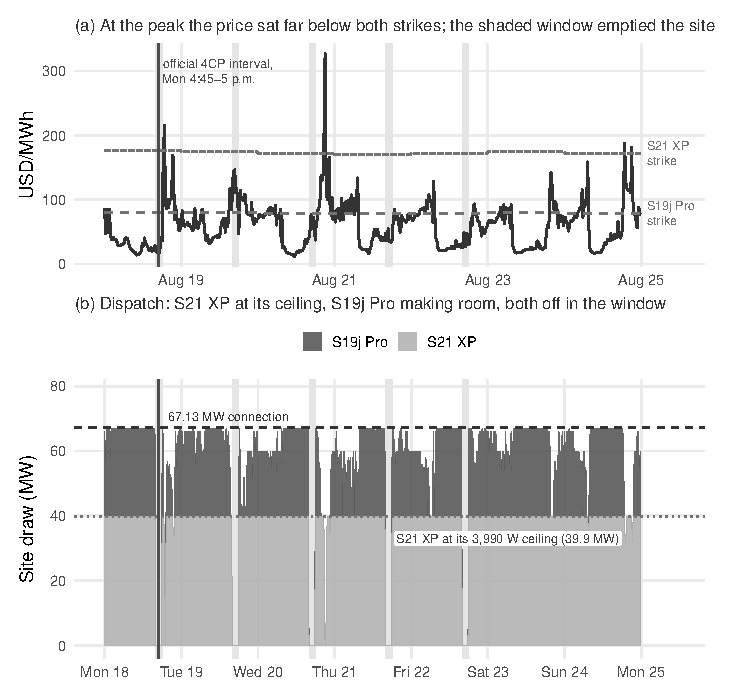
\includegraphics[width=\textwidth]{images/ch9_dispatch_week}
  \caption{One summer week, two fleets, one connection: August 18 to 24, 2025, at LZ\_WEST, the week that holds the month's official 4CP interval. (a)~The settlement price against the two strikes; the price never reached the S19j~Pro's strike in the official interval, which the summer window (shaded) caught anyway. (b)~The dispatched megawatts: the S21~XP pinned at its 3,990~W ceiling through 92~percent of the week, the S19j~Pro running below stock to make room under the connection for 85~percent of it and off for 15~percent, six points of it in the window, when both fleets were dark. At stock power the fleets would draw 30.68~MW (S19j~Pro) and 36.45~MW (S21~XP).} % fig-src: analysis/figures/fig_ch9_dispatch_week.R on analysis/data/ch9_dispatch_week_2025.csv (ch9_optimal_stack.R console: window applied as the planned site plays it; site mean 57.4 MW; S21 XP at ceiling 92%; S19j Pro below stock but on 85%, off 15%, window 6% of the week)
  \label{fig:stack-week}
\end{figure}

Figure~\ref{fig:stack-week} shows the stack physically, in one August week of 2025. The efficient fleet sits at its ceiling almost every quarter-hour. The old fleet runs below stock to fit under the connection and switches off only when the price climbs well past its strike. On Monday afternoon the summer window empties the site while the price, at about \$18 in the quarter-hour ending at 5~p.m., is nowhere near either strike, and that quarter-hour turns out to be the month's official peak. % src: analysis/data/ch9_dispatch_week_2025.csv (official interval 2025-08-18 16:45-17:00, ERCOT label 17:00, at $17.76/MWh; strikes about $79 / $173 that week); ch9_optimal_stack.R console, dispatch week line; the old fleet on the loop's last settlement price, the same csv: outside the window off in 59 quarter-hours, every one after a price of $97.80 or more, at least 1.24 times strike19 ($77.85 to $80.66 that week, the nameplate strike panel (a) draws), and on at 12 to 20 MW in 95 quarter-hours after the price had passed strike19, up to $100.55, against 20 to 27 MW below it; 29.5 / 23.83 = 1.24, the breakeven at its most efficient power target (ch9_flexibility_stack.R console, Layer 4: best 23.83 J/TH at 1200 W; sec:stack-power-target); until 2026-10-04 this line said it "switches off when the price climbs toward its strike"

The strategy, then, is an order of switching, which Section~\ref{sec:stack-rule} states as a procedure. Inside the year it runs with no look-ahead at all. The two annual switches are the only choices the ledger could have made with hindsight, and the headline sets them in advance.

\section{The Other Offer: Behind the Fence}
\label{sec:stack-fence}

Now the second document on the desk. Section~\ref{sec:btm} set the terms: nearly \$9 per megawatt-hour of charges on top of energy, of which a site that dodges the four peaks already escapes about \$5.70, so the fence saves about \$3 against that competent neighbor; the real prize sits on the energy line, between the generator's captured price near \$19 and, on the hours the wind blew, a grid price near \$40. The fence priced here is firm and delivers flat, and for a flat load the grid alternative with the peaks dodged is the \$45 of Chapter~6's table, so the prices tested run from \$19 to \$45. The same section added that an islanded mine forfeits every layer this chapter has just priced. This section prices the forfeit. % src: chapter 6 tab:btm-ledger and sec:btm (analysis/checks/ch6_btm_ledger.R console: energy 42.18; stack 8.83; TCRF 5.65; residual 3.18 islanded; delivered 51.01 / 45.35 flat; top of band 39.90 on wind hours); ch9_optimal_stack.R BAND (19, 45)

The comparison is built on the same engine, with every assumption stated. Both sites use the same fleet and 67.13~MW power budget, with lagged decisions over the same five years. The fenced site pays one negotiated price for every megawatt-hour and nothing else: no losses, no ancillary or uplift allocation, no transmission charge, and, with no grid tie and so no utility meter, no distribution line. It sells no reserves, dodges no peaks, arbitrages no index, and it moves its power targets against its fixed price like anyone else, because the target is firmware. The ledger treats its plant as always available, a gas plant or a firmed contract; a wind-only island would run only when the wind blew, and Chapter~6 already noted that it is least covered at 5~p.m.\ in August. The ledger prices two behaviors of the generator. Under \glossaryterm{firm-supply}{firm supply} the mine runs whenever it wants. Under an \glossaryterm{interruptible}{interruptible} deal the generator keeps the right to switch the mine off whenever the grid pays more than the mine does, sells into the grid instead, and pays the mine nothing for the interruption. The zone price stands in for the plant's node price, which sits lower in West Texas, so the interruptions are overstated. % src: analysis/checks/ch9_optimal_stack.R header (behind-the-meter design; no distribution because it is chapter 6's islanded case, with no grid tie and no utility meter to bill, chapter-6.tex:74 and :80) and console
The question for each year is the \glossaryterm{indifference-price}{indifference price}: the negotiated price at which the fenced site earns exactly what the grid site earns. Below it the fence wins; above it the grid does.

\begin{table}[htbp]
  \centering
  \scriptsize
  \setlength{\tabcolsep}{1.6pt}
  \begin{tabular}{lrrrrrrrrr}
    \hline
    \textbf{Year} & \textbf{Grid,} & \textbf{Grid,} & \multicolumn{3}{c}{\textbf{Fence, firm, at}} & \textbf{Runs at} & \multicolumn{3}{c}{\textbf{Indifference price vs.}} \\
     & never pause & planned & \$19 & \$30 & \$45 & \$45, int. & planned & hindsight & never \\
    \hline
    2021 & 348.72 & 428.93 & 449.71 & 443.28 & 434.52 & 83\% & 54.56 & none & 191.80 \\
    2022 & 132.43 & 144.37 & 170.41 & 163.96 & 155.17 & 51\% & 63.44 & 57.17 & 84.09 \\
    2023 & 65.49 & 84.78 & 98.71 & 92.26 & 83.47 & 76\% & 42.76 & 41.62 & 75.88 \\
    2024 & 65.91 & 71.15 & 84.35 & 77.88 & 69.08 & 77\% & 41.46 & 39.00 & 50.43 \\
    2025 & 43.00 & 49.77 & 64.45 & 58.00 & 49.23 & 63\% & 44.06 & 44.06 & 55.89 \\
    \hline
  \end{tabular}
  \caption{Grid versus fence, millions of dollars per year and \$/MWh. The grid columns repeat the never-pausing and planned sites of Table~\ref{tab:stack-ledger}. The fence columns are the same fleet behind a firm generator at three negotiated prices, power targets free on both sides. ``Runs at \$45, int.'' is the share of quarter-hours an interruptible deal at \$45 would have left the mine running. The indifference price is the firm price at which the fence matches the grid site: against the planned site, against the hindsight ceiling, and against the never-pausing site; ``none'' means no positive price would do. Biases, each stated with its direction: firm always-available supply favors the fence; the zone price as the generator's alternative overstates interruptions; the 2025 charges held for every year flatter the grid site in 2021 to 2023, when allocations were higher; the fence's interconnection, study and legal costs fall on its discount and are not priced.} % tab-src: analysis/data/ch9_btm_indifference.csv (references planned, hindsight, never; firm) and ch9_optimal_stack.csv, written by analysis/checks/ch9_optimal_stack.R; run shares from its console ("interruptible runs" at P = $45: 83% / 51% / 76% / 77% / 63%)
  \label{tab:stack-fence}
\end{table}

\begin{figure}[htbp]
  \centering
  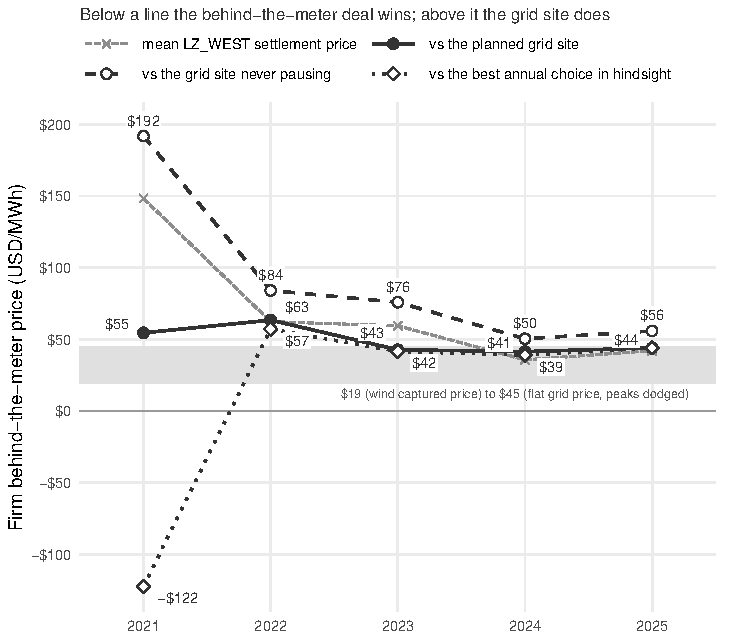
\includegraphics[width=\textwidth]{images/ch9_btm}
  \caption{Where the fence breaks even. The firm negotiated price at which a behind-the-meter site earns what the grid site earns, year by year, against the planned site (solid), against the hindsight ceiling (dotted) and against the same site never pausing (dashed); the mean LZ\_WEST settlement price for reference; shaded, the prices tested, from the wind captured price to the flat grid price with the peaks dodged. Both sites run the same 67.13~MW fleet and power budget, with power targets free on both sides; the behind-the-meter site pays no losses, ancillary, uplift, distribution or TCRF charges and sells no reserves. The planned grid site sets its annual switches in advance. Only the hindsight ceiling of 2021, a grid site that sold RRS through the February storm, has no positive answer.} % fig-src: analysis/figures/fig_ch9_btm.R on analysis/data/ch9_btm_indifference.csv
  \label{fig:stack-btm}
\end{figure}

The comparison in Table~\ref{tab:stack-fence} and Figure~\ref{fig:stack-btm} depends on the grid-site baseline. Against the never-pausing grid site the fence wins at any price in the range in every year: the indifference prices are \$192, \$84, \$76, \$50 and \$56, all above its top, as expected of a site that pays every spike and every peak and never moves its power target. Against the planned site the fence also wins everywhere in the range in 2021 and 2022, where the indifference prices are \$55 and \$63. In 2023, 2024 and 2025 they are \$43, \$41 and \$44, near its top, so a firm deal in the twenties or thirties still beats the stack and one at \$45 does not. Only the hindsight ceiling puts the storm year out of reach: the fence would have had to be paid \$122 for every megawatt-hour it took to match a site that sold reserves through Uri. Against the ceiling the other four years sit at most \$6 lower, at \$57, \$42, \$39 and \$44. % src: analysis/data/ch9_btm_indifference.csv (firm: 54.56, 63.44, 42.76, 41.46, 44.06 vs planned; -122.35, 57.17, 41.62, 39.00, 44.06 vs hindsight; 191.80, 84.09, 75.88, 50.43, 55.89 vs never); the never-pausing site's delivered price, ch9_optimal_stack.R console PER MWh lines, mean energy price plus its charges (it draws flat, so it pays the time-weighted mean): 148.33 + 10.24, 62.35 + 8.37, 59.42 + 8.31, 35.71 + 7.78 = $43.49 in 2024 and 42.18 + 7.94 = $50.12 in 2025; 2024 at $45 the firm fence earns $69,078,122 against never pausing's $65,911,448 (+4.8%, the "at P = $45" line), but at stock power it would trail: revenue before energy $91,519,083 (2024 FIRMWARE FEE line) less 45 x 588,528 MWh (67.00 MW at the curves' stock points x 8,784 h) = $65.04M; until 2026-10-04 this line said the never-pausing site "pays a delivered price above $45" in every year
In 2022, 2024 and 2025 a firm price in the twenties or low thirties beats everything the grid site can plan with its switches, because the stack was worth \$9 to \$20 per megawatt-hour and the discount below the zone price plus the avoided charges was worth more. In the storm year the planned site's stack was worth \$137 per megawatt-hour on a \$148 average price, and a firm fence at \$45 still beat it, because a firm deal buys Uri's week at \$45, the first of the biases the table's caption names. Only the reserve award of the hindsight ceiling, \$313 per megawatt-hour, put the grid site beyond any discount. % src: ch9_optimal_stack.R console, PLANNED lines (flexibility per MWh: 2022 $20.31, 2024 $8.89, 2025 $11.52; 2021 $136.76), 2021 HINDSIGHT CEILING line ($313.07) and mean price (2021 $148.33); 2021 firm BTM profit at $45 $434,517,092 vs planned grid $428,927,595; until 2026-10-04 this line said "the planned site earned $137 per megawatt-hour", its flexibility, not its margin, which was $731 per MWh ($428,927,595 / 586,448 MWh)
The fence is an annuity: a discount on every megawatt-hour, the same in a storm as on a Tuesday in April. The stack is an option: thin most of the time, and worth years of the annuity in Uri's week, under a cap since lowered (Section~\ref{sec:ordc}).

The second finding is about the switch, not the price, and it is the reason the firm case is a ceiling. An interruptible fence, where the generator takes the power back whenever the grid pays more than the mine does, matches the planned site at no price in any of the five years. At \$19 in 2025 such a mine would have run 24~percent of the year; at \$45, 63~percent; the best it could do at any price, about \$32~million at a price near \$55, is a third short of the grid site's \$50~million. % src: ch9_optimal_stack.R console, "interruptible" lines (matches the planned grid site up to P = no price in every year; 2025 runs 24% at $19, 45% at $30, 63% at $45; best case $31,954,770 at P = $55; planned grid $49,772,629)
Every hour the grid pays more than the contract is an hour the fenced mine goes dark for nothing: every hour in which the grid site's pause is worth money, and every hour between the contract price and the strike in which the grid site mines at a profit. The sell option Chapter~6 valued in Section~\ref{sec:ownergen}, about \$960,000 per megawatt-year for the S19j~Pro in 2021 and \$51,000 in 2025, has moved to the generator's side of the fence. % src: analysis/checks/sell_vs_mine.R console, moving-strike table (2021 $957,665; 2025 $51,499 per MW-yr), as quoted in chapter 6 sec:ownergen, the S19j Pro's; the S21 XP's same-interval option was smaller, 31,320,751 / 36.45 MW = $859,280 and 675,521 / 36.45 = $18,533 per MW-yr (ch9_flexibility_stack.R console, "The price of not seeing the future", foresight gains); until 2026-10-04 this line named no fleet
A generator that keeps the switch sells the mine electrons and keeps the option; a mine that keeps the switch sells its flexibility to the grid.
Firmness matters alongside price in a behind-the-meter deal. A firm price in the lower half of the \$19 to \$45 range beat the planned site in every one of the five years, and firmness through a storm week is exactly what no generator gives away at \$45. % src: analysis/data/ch9_btm_indifference.csv (firm BTM profit at $19 and $30 above the planned grid site in every year; the 2021 row above)

The filings show what the industry has concluded from the same arithmetic, and it is neither pure case. Hut~8's Vega site runs behind a wind farm and in front of the grid at once; Soluna's Dorothy sits behind a plant it does not own and still earned demand-response revenue; Riot's fixed-price contracts with sell-back rights produced \$54~million of curtailment credits in 2025. % src: chapter 6 sec:btm (hut8_10k2025; soluna10k2025 $1.285M; riot10k2025 $54.302M manual curtailment credits)
The hybrid buys the annuity and keeps the option. The companion repository holds no generator-availability data, so the hybrid is described here and not modeled; its economics are, at best, the firm fence's margin in Table~\ref{tab:stack-fence} plus the strike and any reserves, the two layers only a grid tie adds, less whatever the generator charges for letting the mine keep its switch. % src: tab:stack-fence fence columns (power targets free on both sides; no transmission charge, so the summer window has nothing left to save); until 2026-10-04 this line added "the planned site's flexibility and the firm fence's discount from Table 9.3", a discount the table does not print, whose natural reading, a fence column less the never-pausing one, already holds the fence's own power target, and whose energy and charges include the transmission charge the flexibility's window also counts (2025 at $45: fence $49.23M less never pausing $43.00M = $6.23M, about $3.0M of it the discount, (42.18 + 7.94 - 45) x 588,059 MWh, ch9_optimal_stack.R console PER MWh line, and about $3.2M the power target)

\section{The Decision Rule}
\label{sec:stack-rule}

% layout (2026-10-05): this, the \looseness on step 7 and the enlargement before "The parts were worth less" keep chapter 9's last lines off a page of their own; revisit if the text above changes
\enlargethispage{2\baselineskip}
For a site of your own, the chapter reduces to eight steps.

\begin{enumerate}
  \item Compute each machine model's strike every day: yesterday's hashprice times 41,667, divided by the model's joules per terahash.
  \item Keep the pause alive: take-or-pay without resale only at a discount above the flexibility lost. If you index, index real time.
  \item Run one strike per model with the three rules of Chapter~5. Never blend the fleets into one site strike.
  \item Move the power target, and size the connection just under 75~MW, counting every load at the site. % src: sec:stack-power-target, the design-brief sentence (75 / 1.10 = 68.18 MW of machines at most, chapter-1.tex PUE 1.10; this fleet's full tilt 74.10 MW, 81.5 MW at the meter); until 2026-10-04 this step said "size the connection for full tilt below 75 MW", written when the brief sized the connection for the machines alone (PER-3 moved the brief to every load at the meter and left "for full tilt" here)
  \item Decide the summer window on June~1. Play it only if your fleet's power-weighted margin, the strike on yesterday's hashprice less last summer's window price, is under the transmission prize divided by the window's hours. Budget no transmission saving before the year after a new site's first full summer: until then the wires utility bills it on an estimate \autocite{oncor2026retailtariff,centerpoint2026retailtariff}. Never sell the emergency program's afternoon block.
  \item Decide reserves interval by interval, through your load resource's QSE (Chapter~7). Under RTC+B a day-ahead award can be bought back at the real-time reserve price. When the price beats your strike by more than that buyout, telemeter your reserve away, then pause once the five-minute run stops awarding it. Never sell the window's hours. Expect little: every rule set in January that said sell lost to never selling.
  \item \looseness=-1 Take a fence offer only if it is firm and its price is below the indifference price your own numbers produce. Walk away if the generator keeps the right to interrupt without paying for it, or if the deal islands the site; a fence with a grid tie is the hybrid of Section~\ref{sec:stack-fence}. Clear the netting rules of Section~\ref{sec:btm} before you sign.
  \item Run the calculator in the companion repository for your zone and contract, with your fleet as a mix of its two machines, and read the friction line in its footer.
\end{enumerate}

% layout (2026-10-04): lets the chapter's last page run long so its final lines do not spill onto a page of their own; move or drop if the text above changes
\enlargethispage{3\baselineskip}
The parts were worth less together than a brochure would add them up to. The size of the prize was set by hashprice and the market's regime, not by the grid's generosity.

Three things move after the data ends, and Chapter~10 takes them up. RTC+B, which step~6 already assumes, turns reserves into a priced option rather than an either/or. 12CP and the minimum billing demand, if adopted as proposed, would shrink or end the peak layer. And hashprice, which sets every threshold in this chapter, rests on a subsidy that halves on a schedule.


\part{Outlook}

\chapter{What Comes Next}
\label{ch:outlook}

A reader who came to this book from the Bitcoin side brought one question to page one, and it is time to answer it: does the grid save mining, or does mining serve the grid? Nine chapters have said, in effect, both, and the ledger of Chapter~9 priced what serving the grid was worth to one site over five years. This last chapter looks forward through arithmetic the reader can check. Three sums carry the chapter. The first is what happens to the flexibility stack if hashprice keeps falling as future halvings cut the subsidy. The second is the block subsidy set against any path the price of bitcoin can plausibly take. The third is the \glossaryterm{security-budget}{security budget}, what the network pays for the hashes that protect it, and who will pay it when the subsidy is gone. Chapter~9 handed this chapter three things whose rules change after its data ends, and each gets its place: RTC+B, which turned reserves into a priced option; 12CP and the minimum billing demand, which, if adopted as proposed, end the peak layer for new large loads; and hashprice, which rests on a subsidy that halves on a schedule. One convention is fixed here for the whole chapter. Where a dollar figure depends on the price of bitcoin, it uses \$81,273, the last price in the companion repository's daily series, on September 4, 2026; Chapter~4 used the August price of about \$66,000. Every such line scales in proportion, so the reader can rescale it on the day they read, and none of it is a price forecast: Chapter~5 explained why forecasting is not this book's habit. Every prediction here is my reading of those three sums, labeled as such, and you can run them with other numbers in the companion repository. % src: analysis/checks/ch10_subsidy_arithmetic.R console (reference price $81,273 on 2026-09-04, blockchaininfocharts); chapter 4 ($66,180 seven-day mean to 2026-08-21, analysis/data/btc_price_daily.csv); chapter 9 sec:stack-rule (the three hand-offs)

\section{The Cheaper the Hash, the Better the Grid Resource}
\label{sec:outlook-cheaper}

Chapter~9 found that the old machine did most of the site's grid work. The S19j~Pro, with a strike of \$72 in 2025, paused 14~percent of the year and earned nearly three times as much from the strike per megawatt as the S21~XP, whose strike of \$157 sat above almost every price the year produced. % src: chapter 9 sec:stack-strike (paused 14% vs under 3%; per MW-yr 45,983 vs 15,938 = 2.9x)
That asymmetry follows from where any machine's strike sits relative to the power price, and the strike is hashprice times 41,667 divided by efficiency, Chapter~4's identity. Every machine's strike falls with hashprice, and hashprice fell six-fold from 2021 to 2025. So what does the stack of Chapter~9 look like as every machine becomes what the S19j~Pro is today? % src: chapter 4 (the 41,667 identity); chapter 9 sec:stack-site (spliced hashprice $0.310 in 2021 to $0.051 in 2025)

Here, the ``optimal site'' uses the price-response loop and plays the summer window where it pays over the modeled year. The loop acts on past prices; the annual window choice uses the year's results.

\begin{figure}[htbp]
  \centering
  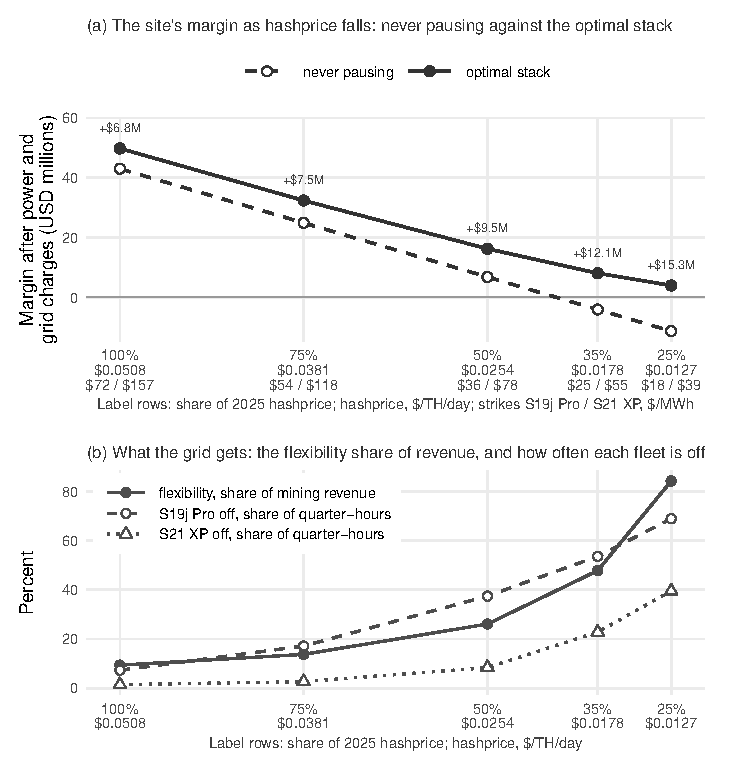
\includegraphics[width=\textwidth]{images/ch10_hashprice_sensitivity}
  \caption{Chapter~9's reference site on 2025 LZ\_WEST prices, with the daily hashprice scaled from 100 to 25~percent of its actual path. (a)~Margin after power and grid charges of the never-pausing site against the optimal stack; the axis carries the share, the hashprice in dollars per terahash-day and the two strikes; the label on each point is the value of flexibility. (b)~Flexibility as a share of mining revenue, and the share of quarter-hours each fleet spends switched off under the optimal stack; with the power target available the site prefers to underclock rather than stop, so the off share sits below the pause share of a plain strike rule. Lagged decisions, measured power curves and 2025 grid charges; the summer window is played where it pays, and reserves are left aside.} % fig-src: analysis/figures/fig_ch10_hashprice_sensitivity.R on analysis/data/ch10_hashprice_sensitivity.csv (ch10_hashprice_sensitivity.R)
  \label{fig:outlook-sensitivity}
\end{figure}

Figure~\ref{fig:outlook-sensitivity} and Table~\ref{tab:outlook-sensitivity} rerun the 2025 ledger with hashprice scaled down, everything else unchanged: the same prices, lagged loop and charges, the summer window played where it pays. At the actual 2025 hashprice, flexibility was worth \$6.8~million, 15.8~percent of the never-pausing site's margin and 9.4~percent of its mining revenue, Chapter~9's ledger row. At three quarters of that hashprice, where the S19j~Pro's strike falls to \$54, flexibility is worth \$7.5~million and 30.0~percent of margin. At half, with strikes of \$36 and \$78, the never-pausing site earns \$6.8~million and the optimal site \$16.2~million: the stack is worth more than the business it sits on. At 35~percent of the 2025 hashprice the never-pausing site loses \$4.1~million and the optimal site still earns \$8.1~million; at a quarter, the loss is \$11.3~million against a margin of \$3.9~million. % src: analysis/checks/ch10_hashprice_sensitivity.R console (never / optimal / flexibility, USD millions: 43.00 / 49.77 / 6.77, and 6.77 / 43.00 = 15.8% of profit; 24.89 / 32.37 / 7.48, 30.0% of profit; 6.79 / 16.24 / 9.45; -4.07 / 8.05 / 12.13; -11.32 / 3.95 / 15.26; shares of revenue 9.4 / 13.8 / 26.1 / 47.8 / 84.3%; the prose printed 30.2%, $16.3 million, $8.2 million and a margin of $4.1 million (16.30, 8.16, 4.10) until 2026-10-03, when the ledgers booked distribution at $0.50 per MWh consumed; the 2025 ledger on all 8,760 h since chapter 9's hashprice loader filled the gap of 2025-11-13 to 15)
Down to half the 2025 hashprice, where the site still covers its power and grid charges without pausing, flexibility grows in dollars and in share as the margin it protects shrinks. That margin reaches zero at about 41~percent of the 2025 hashprice. A site that must also pay for its machines, its staff and its debt crosses that line sooner: every \$100,000 a megawatt-year of such costs raises it by about 9 points. % src: analysis/checks/ch10_hashprice_sensitivity.R console, margin crossover line (1 - 42,997,846 / 72,419,582 = 40.6% of the 2025 hashprice, never_total and revenue_stock of the 100% row of analysis/data/ch10_hashprice_sensitivity.csv, which is linear in hashprice; 100,000 x 67.13 / 72,419,582 = 9.3 points)
Below that line, flexibility can determine whether a site covers its power and grid costs. Section~\ref{sec:outlook-payers} examines what that flexibility is worth to the grid.

\begin{table}[htbp]
  \centering
  \scriptsize
  \setlength{\tabcolsep}{1.8pt}
  \begin{tabular}{lrrrrrrrr}
    \hline
    \textbf{Hashprice} & \textbf{\$/TH/day} & \textbf{Strikes} & \textbf{Never} & \textbf{Optimal} & \textbf{Flex.} & \textbf{Share of} & \textbf{S19j} & \textbf{S21} \\
    vs.\ 2025 & & S19j / S21 & \$M & \$M & \$M & revenue & off \% & off \% \\
    \hline
    100\% & 0.0508 & 72 / 157 & 43.00 & 49.77 & 6.77 & 9.4\% & 7.3 & 1.4 \\
    75\% & 0.0381 & 54 / 118 & 24.89 & 32.37 & 7.48 & 13.8\% & 17.1 & 2.7 \\
    50\% & 0.0254 & 36 / 78 & 6.79 & 16.24 & 9.45 & 26.1\% & 37.5 & 8.4 \\
    35\% & 0.0178 & 25 / 55 & $-$4.07 & 8.05 & 12.13 & 47.8\% & 53.6 & 22.8 \\
    25\% & 0.0127 & 18 / 39 & $-$11.32 & 3.95 & 15.26 & 84.3\% & 68.9 & 39.6 \\
    \hline
    2026, 8 mo.* & 0.0338 & 48 / 104 & 16.45 & 20.06 & 3.60 & 11.3\% & 10.0 & 2.4 \\
    \hline
  \end{tabular}
  \caption{The stack as hashprice falls. Chapter~9's 67.13~MW site on 2025 LZ\_WEST prices, with the daily hashprice scaled; the second column is the year's mean hashprice in dollars per terahash-day at that scale; ``never'' is the never-pausing site's margin after power and grid charges, ``optimal'' the price-only stack (strike, power target, summer window). ``Off'' is the share of quarter-hours a fleet draws nothing under the optimal stack. The first row is Chapter~9's 2025 ledger. Flexibility as a share of the never-pausing margin is 15.8, 30.0 and 139~percent in the first three rows and has no meaning once that margin is negative. Without the summer window, which the proposed minimum billing demand would take from a new load of 75~MW or more, flexibility is 5.17, 5.47, 7.06, 9.53 and 12.56~million dollars in the first five rows. *The last row is the actual first eight months of 2026 under RTC+B, without the summer window because the year's official peaks are not yet known; its \$M columns cover 241 days, not a year (pro rata about \$24.9, \$30.4 and \$5.5~million, on months that hold Fern and the summer but no autumn), so it compares with the rows above by its shares (21.9~percent of margin). Strikes in \$/MWh.} % tab-src: analysis/data/ch10_hashprice_sensitivity.csv, written by analysis/checks/ch10_hashprice_sensitivity.R (without the window: flex_nowin_value 5,167,912 / 5,465,476 / 7,058,241 / 9,528,489 / 12,556,893 in the 100 to 25% rows; share of margin flex_pct_profit 15.8 / 30.0 / 139.2; the table's figures moved on 2026-10-03, when the ledgers stopped booking distribution at $0.50 per MWh consumed and billed it on each month's peak, from 42.98 / 49.78 / 6.80, 24.88 / 32.39 / 7.52, 6.77 / 16.30 / 9.53, -4.09 / 8.16 / 12.24, -11.33 / 4.10 / 15.43 and 3.62, revenue shares 26.3 / 48.3 / 85.2 / 11.4%, margin shares 30.2 / 140.6 / 22.0%, without the window 5.19 / 5.50 / 7.13 / 9.64 / 12.72; the minimum's reach per chapter 8 sec:twelvecp); 2026 row: hours 5,783 (241 days less the spring-forward hour); console line "2026 pro rata" (x 8,760 / 5,783 = 1.515: never 24.92, optimal 30.38, flexibility 5.46 $M), linear, with no seasonal adjustment
  \label{tab:outlook-sensitivity}
\end{table}

Two strike thresholds mark how far hashprice has to fall. The S21~XP inherits the S19j~Pro's 2025 strike when hashprice falls to 46~percent of its 2025 level, \$72 over \$157; the S19j~Pro's own strike falls below the year's mean price at 59~percent. A subsidy halving does not by itself decide either crossing: hashprice also depends on bitcoin's price, transaction fees and network hashrate, as Chapter~4 explains. % src: ch10_hashprice_sensitivity.R console, crossovers (71.73 / 156.74 = 0.46; 42.18 / 71.73 = 0.59)
The off share is not Chapter~9's pause share: with the power target the site underclocks before it stops, so the S19j~Pro that paused 14~percent of 2025 under the plain strike rule drew nothing in 7~percent of quarter-hours under the stack. Read the two ``off'' columns with that in mind. At the 2025 hashprice the S21~XP is off for 1~percent of the year; at half that hashprice, for 8~percent, about the S19j~Pro's off share in 2025; at a quarter, for 40~percent. The site's mean draw falls from 62.9~MW to 30.3~MW across the same rows. The site uses less energy, but a larger share of its megawatts moves on the price signal, and the energy it does use comes from the bottom of the price curve. % src: ch10_hashprice_sensitivity.R console, mean draw (62.9 / 59.0 / 51.0 / 40.7 / 30.3 MW)
The efficient machine of today becomes the flexible machine of tomorrow without changing a chip, because what makes a machine flexible is not its silicon but the distance between its strike and the price. And the first eight months of 2026, the first under RTC+B, are already a step down that path. Hashprice took the S19j~Pro's strike to \$48. In those eight months the never-pausing site would have earned \$16.5~million and the optimal site \$20.1~million, a difference of 22~percent of margin with no summer window counted yet, more than 2025's 16~percent. Part of that is Winter Storm Fern in January, a scarcity month of the kind Chapter~9 showed inflates the value of the switch, so the eight months are consistent with the path rather than proof of it. % src: ch10_hashprice_sensitivity.R console, 2026 row (241 days of data, Jan 1 to Aug 29, every day since chapter 9's hashprice loader filled the gap of Aug 17-23; hashprice 0.0338; strikes $48 / $104; never $16.45M, optimal $20.06M, flexibility $3.60M = 21.9% of profit, 11.3% of revenue); chapter 2 (Fern, January 2026)
The table rests on these assumptions. Prices are 2025's, held fixed while hashprice moves; each hashprice level is held for a whole year; Chapter~4's difficulty loop is not modeled, so the 35 and 25~percent rows describe what a site faces at that level, not how long the level lasts; the machines are those of the 2026 fleet dataset, with no newer model among them.

A fleet that is off about 40 or 70~percent of the year hashes about 40 or 70~percent less, and if a large share of the network did the same in the same hours, blocks would come slower than every ten minutes in those hours and the difficulty adjustment would follow them down. Is that a threat to the coin's issuance or its security, and does the protocol need something new to meet it? Issuance is safe by construction: coins are issued per block, not per minute, so slower blocks delay the schedule inside a two-week difficulty period, and the difficulty adjustment, which resets difficulty to whatever hashrate the network averaged over the previous 2,016 blocks, restores the ten-minute cadence at the next boundary. That adjustment is the protocol's answer, and it was built for exactly this. Winter Storm Fern was the test at scale: Texas curtailment took roughly 200~EH/s offline, the next adjustment was the largest fall since the 2021 China ban, 11~percent, and the one after it rose 15~percent as the machines came back (Chapter~2). % src: chapter 2 (Fern: ~200 EH/s offline at U.S. pools; difficulty -11.16% on Feb 7, 2026; +14.7% after); chapter 4 (the difficulty loop); protocol: 2,016-block retarget
Flexibility changes how the network's security is spread across the hours. Difficulty is only a measurement; what protects the chain at any moment is the hashrate applied at that moment, and a flexible network applies the fewest hashes in exactly the hours when power is scarcest. How far that goes depends on how synchronized the pauses are, which is a question of geography. ERCOT's mining demand at its 2025 peak, roughly 4,600~MW (Chapter~7), becomes a share of the network's hashrate only through an efficiency, and the one that counts is Texas's own, not the network's. This book assumes the Texas fleet runs at 17 to 21.5~J/TH at the machines, from the listed fleets' average to my estimate for the whole network (Chapter~1), with a tenth more drawn at the meter. On that assumption Texas holds a fifth to more than a quarter of the network's hashrate at full output. If every Texas mine paused at once, as much of it did in Fern, blocks would stretch to about twelve and a half to thirteen and a half minutes until the next difficulty adjustment. An attacker who could time their work to those hours would face a network a fifth to more than a quarter weaker than its average. If the whole Texas fleet ran the dispatch of Table~\ref{tab:outlook-sensitivity} at a quarter of the 2025 hashprice (off for 55~percent of its energy but only 47~percent of its hashes, because a lowered power target sheds energy faster than hashes), the network's average hashrate would sit about 10 to 12~percent below the same machines always on. At 2025's hashprice the same dispatch saves 6~percent of the site's energy and gives up no hashes at all on balance. The power target runs the machines above stock in cheap hours about as much as it holds them below stock in dear ones. % src: ch10_hashprice_sensitivity.R console, synchronized curtailment (Texas hashrate = 4,600 MW / PUE 1.10 / J_TX: 246 EH/s = 26.5% of 930 EH/s at 17 J/TH, 195 EH/s = 20.9% at 21.5 J/TH; 10 / (1 - share) = 13.6 and 12.6 min; 25% hashprice: energy off 55%, hashrate off 46.7%, share x 46.7% = 12.4% and 9.8%, 14.5% and 11.5% on the old energy basis; 2025: energy off 6%, hash share 1.002 of stock, analysis/data/ch10_hashprice_sensitivity.csv hash_share); J_TX 17 to 21.5 J/TH is an assumption proposed in DATA-017 (2026-09-26), pending the author's confirmation, and is printed as the book's assumption, not the author's reading: 17 is the listed fleets' hashrate-weighted average (analysis/checks/ch1_fleet_efficiency.R), not a Texas figure, 21.5 the author's estimate for the network (chapter 1); the two fleets the repository places in Texas, Riot (42.5 EH/s at 20.2 J/TH; Rockdale, Corsicana and also Kentucky) and Cipher's Odessa site (11.6 EH/s at 17.2), both on Q1 2026 J/TH flagged stale, weight to 19.56 J/TH (analysis/data/listed_miner_fleets_2026.csv; ch10_hashprice_sensitivity.R console, "Texas fleets in the repository" and the 19.6 J/TH line: 23.0%, 13.0 min, 10.7%), so the efficient end sits below Texas's own disclosed fleets; it is kept as the efficient bound because the other listed fleets report only fleet-wide figures, so the Texas fleet as a whole is not known to be less efficient than the listed average; PUE 1.10 is CBECI2026's best guess, because the 4,600 MW is metered site demand; chapter 7 opening (potomac2026somercot pp. i, 31, ~4,600 MW, the 2025 peak of aggregate mining demand; a capacity-like basis, so the shares are shares at full output); until 2026-09-26 this sentence divided the 4,600 MW by chapter 1's old 24.2 GW, taking Texas at the network's average (a fifth, twelve minutes, 9 percent; DATA-017). Was 5,768 MW until 2026-09-20, which is chapter 3's large-load PROGRAM total across all industries, not mining; both sentences here are about mining, so the monitor's figure is the right input
Against that stands the other half of the same arithmetic: the same security budget buys more hashes in total when a mine takes the cheap hours and leaves the dear ones, so a flexible network has a higher average hashrate per dollar and a lower floor. The floor needs no change to the protocol, because the difficulty adjustment already absorbs a varying hashrate and Fern showed it absorbing a Texas-sized swing within two weeks. The exposure that matters is correlation, every grid's scarce hours falling at once, and the defense against that is not in the code but on the map, a network spread across grids whose scarce hours differ. That is one more reason to expect the mines that survive the halvings to be dispersed, and to be on grids whose peaks do not coincide.

This is the first of the chapter's three sums, and it is the one that answers the bitcoiner's question from the grid's side. The grid does not save mining. It pays mining for a product, and the product gets larger, relative to everything else the mine earns, every time hashprice falls. Each halving cuts the subsidy, but the resulting hashprice also depends on bitcoin's price, fees and network hashrate. Section~\ref{sec:outlook-halving} asks how long price growth can offset the subsidy cuts.

\section{A Standard Part of the Grid, Beside the Batteries}
\label{sec:outlook-grid}

The grid's side of the ledger is easier to read forward than the miner's, because the grid has said what it wants. ERCOT's queue of prospective large loads stood near 410~GW in early 2026 and near 474~GW by that August, about 90~percent of it data centers \autocite{abbott2026datacenters}. That is more than five times the record peak demand, which first passed 90~GW in July 2026 (Chapters~3 and~8). % src: chapter 3 sec:miners-ercot (vegas2026senateupdate, April 2026: 410,618 MW tracked, 87.6% data centers); abbott2026datacenters (governor's letter, August 3, 2026: "approximately 474 gigawatts", "more than five times Texas' record peak", "approximately 90 percent ... are data centers"), quoted at origin; the two figures are four months apart and the sentence prints both as a trajectory; chapter 8 sec:fourcp-peaks (91.2 GW on July 22, 2026)
A queue counts requests, not load. Of those 410~GW, 294~GW belonged to requests that had not yet given ERCOT enough information to begin a review, or had been reviewed and not approved, and under 6~GW had been energized \autocite{vegas2026senateupdate,ercot2026llistatus}. % src: vegas2026senateupdate slide 3 table (as of March 26, 2026, through 2030: 410,618 MW total, 293,651 MW No Studies Submitted, 5,778 MW Observed Energized); ercot2026llistatus slide 3 (No Studies Submitted: projects that "have not yet provided sufficient information for ERCOT to begin review", plus "MWs that were not approved by ERCOT after review of planning studies")
When ERCOT sorted the requests for its first batch study in September, 302~GW of them, 373 projects, conditionally failed to qualify and had to wait for a later study; the verdict was set to become final only after a verification and audit due in December \autocite{ercot2026batchzero,ercot2026ltlfadjust}. % src: ercot2026batchzero slides 1, 4, 6 (conditional classification sent to the TSPs September 3, 2026; excluded 302.2 GW, 373 projects; base 66.4 GW, 204 projects; studied 125.4 GW on slide 6 but 127.9 GW on slide 1, so neither prints; Eligibility Verification Report due December 10, 2026, final inclusion or exclusion then); ercot2026ltlfadjust pp. 5-6 and fn. 10 (loads outside the eligibility criteria are "ineligible to receive approval for Initial Energization until evaluated through a future interconnection study process", PGRR145 as proposed; PUCT approval of PGRR145 on June 18, 2026, ercot2026batchzero slide 2); the batch covers 494 GW over 2028-2032, not a subset of the 410 GW, so the sentence does not say "of those"
What ERCOT planned for was a forecast, and a smaller one: in 2025 it discounted the loads the utilities reported by what such loads had actually delivered, since data centers due in 2022 to 2024 had drawn half of what they requested. So it cut the 208~GW peak the utilities' reports implied for 2030 to 138~GW, existing load included, inside the 130 to 148~GW range its 2024 transmission plan had used \autocite{ercot2025ltlf}. % src: ercot2025ltlf slide 9 (data centers with 2022-2024 in-service dates: load 49.8% of the requested amount; officer-letter loads 55.4% in service by February 2025; in-service about 220 days late on average), slides 10-11 (TSP-provided 2030 peak 208 GW; ERCOT-adjusted 2030 peak 138 GW, 94,145 MW of base load included; "130 GW to 148 GW range used in 2024 Regional Transmission Plan for forecast year 2030")
When the utilities' reports lifted the 2026 preliminary forecast to 368~GW by 2032, ERCOT's chief executive said ERCOT believed it was ``higher than expected future load growth,'' and ERCOT asked the commission to cut it \autocite{ercot2026ltlfprelim,ercot2026ltlfadjust}. % src: ercot2026ltlfprelim (April 15, 2026: "approximately 367,790 MW of demand in the ERCOT Region by 2032"; Vegas quote verbatim; the forecast "is not a prediction of what will be built"); ercot2026ltlfadjust pp. 1-2, 7 (May 18, 2026: request under 16 TAC 25.370(e)(2)(B) to adjust the forecast "to a more realistic forecast", Batch Zero option recommended); its 32% realization-rate figure does not print, since its own Table 1 cuts 2032 from 367,790 to 201,662 MW, 45% of the whole forecast
The Duke study that miners now quote back to regulators put a number on what flexibility is worth to a system in that position. Across the United States, about 76~GW of new load could connect without new generation if it accepted curtailment of a quarter of one percent of the energy it could draw in a year, 98~GW at half a percent, and 126~GW at one percent. On the study's average that means 85 to 366 hours a year, most of them partial, in events that average under three hours; ERCOT's share ran from about 6.5~GW at the lowest of those rates to 10~GW at half a percent and 15~GW at one percent \autocite{duke2025rethinking}. % src: duke2025rethinking p. 2 key results and Figure 1 (76 / 98 / 126 GW at 0.25 / 0.5 / 1.0% annual curtailment; 1.7 / 2.1 / 2.5 h average events; ERCOT 6.5 / 10.0 / 14.7 GW); p. 16 (the rate is "the total annual curtailed megawatt-hours divided by the new load's maximum potential annual consumption, assuming continuous operation at full capacity"); p. 20 (1,643 of 657,000 GWh at 0.25%; 85 / 177 / 366 h a year at 0.25 / 0.5 / 1.0%, averaged across the 22 balancing authorities, ~1% of the hours at 0.25%; 88% of those hours keep at least half the new load; "The average duration across BAs was 1.7 hours for the 0.25% limit" to 2.5 hours at 1.0%, an average, so the events "average" under three hours rather than all lasting under three); the key results gloss the rate as "0.25% of their maximum uptime", which this sentence read as hours until 2026-09-26 (PER-3 C10-2); read in the 43-page PDF of February 10-11, 2025 fetched 2026-09-26, the Duke URL since behind a bot check
ERCOT's own words, in a September 2024 presentation on large loads, are that ``the optimal solution for grid reliability is for more Loads to participate in economic dispatch (SCED) as a Controllable Load Resource (CLR),'' the class Chapter~7 described \autocite{springer2024largeloads}. % src: springer2024largeloads slide 32, "Path Forward, More Loads Participating in SCED" (quote verbatim but for the lowercased opening letter and the comma replacing the closing period; ERCOT capitalizes Loads and Controllable Load Resource as defined terms); slide 1 for speaker, title and ERCOT logo
Giving up one percent of its energy is not a stretch for a mine. Chapter~9's S19j~Pro fleet paused between 2 and 17~percent of its quarter-hours on price alone, the S21~XP never more than 3~percent. Under the 12CP rule Chapter~8 describes (Section~\ref{sec:twelvecp}), if adopted as proposed, a site outside the minimum billing demand with a good forecast would sit out on the order of a hundred hours a year to avoid forecast demand peaks, since sitting out the thousand hours that a rule without a forecast needs does not pay. % src: chapter 9 fig:stack-moving-strike (S19j Pro 2.4% in 2021 to 16.7% in 2026 ytd; S21 XP at most 2.7%; a pause of a share of the quarter-hours gives up at least that share of the energy at full capacity, duke2025rethinking's basis, p. 16); chapter 8 sec:twelvecp (1,040 h rule covers 8-11 of the 12 thirty-minute peaks and stops paying; a forecast turns a thousand hours into a hundred; the minimum reaches new or expanding loads of 75 MW or more, not a site already energized on October 8, 2026 that does not expand)

What has changed since the early chapters is the company a mine keeps on the flexible side of the grid. Eighteen gigawatts of batteries compressed the price of standby 61-fold in four years, from a 2021 level that was mostly one storm week (Chapter~7), while the daily price spread compressed by more than a quarter beside them (Section~\ref{sec:batteries}). In the first months under RTC+B the day-ahead price of Responsive Reserve averaged \$1.75 per megawatt per hour of standby against \$2.76 in 2025, ECRS \$2.04 against \$2.46, while Non-Spin, the slow product, rose from \$3.05 to \$3.94. % src: chapter 7 (61-fold, 2021 to 2025; 18 GW); chapter 6 sec:batteries (spread $112 to $82; one year's correlation); ch10_hashprice_sensitivity.R console, 2026 reserve prices (RRS 1.75 vs 2.76; ECRS 2.04 vs 2.46; NonSpin 3.94 vs 3.05 $/MW-h)
On this evidence, a mine is a poor fast reserve. A battery holds a megawatt ready for minutes at almost no cost; a mine that holds a megawatt ready gives up its strike and power-target gains every hour it stands by, and in 2025 standing by lost the either/or in every combination Chapter~9 tried. Whether a mine sells the slow product under RTC+B is open, and the companion repository does not yet price it. What a battery cannot do is what a mine does best: consume. A battery moves about two hours of energy from one part of the day to another and is empty, 1.8 hours of storage on the ERCOT fleet average. A mine can absorb surplus for as long as the surplus lasts, the roughly 490 negative-price hours of 2025 in West Texas among them, and vanish for as long as the shortage lasts, a summer afternoon or a February week. % src: chapter 6 sec:batteries (fleet average 1.8 h of storage); chapter 6 sec:ownergen (about 490 negative-price hours in 2025); chapter 2 (Uri)
The division of labor that follows is the one the market is already pricing: batteries take the minutes and the intraday swing, mines take the hours, the days and the surplus.

RTC+B settles the first of Chapter~9's hand-offs by turning its annual either/or into a rule a site can apply every five minutes. A reserve award is now a financial position that can be bought out at the real-time reserve price. So a site holds the award and mines. When the price less its strike, per megawatt-hour, exceeds the reserve price, it first telemeters its reserve capability away, so that the next five-minute run awards it nothing, and only then pauses (Chapter~7). The position is a premium collected while mining and paid back in the few hours the site pauses. The companion repository holds day-ahead reserve prices, not real-time ones, so this chapter can bound the rule's cost but cannot price a year of it. Chapter~8 priced a two-hour buyout, at day-ahead prices, at under \$160 per megawatt on fourteen of the twenty official 4CP afternoons of 2021 to 2025 (Section~\ref{sec:fourcp-econ}). The market monitor's first full assessment of RTC+B is a year away. What the first eight months did show is the value of a pause under the new market. Price-only, with no summer window on either side, flexibility was worth \$8.79 per megawatt-hour of the site's capacity in 2025 and \$9.28 in 2026 to date, on a mean price a quarter lower and with twice as many negative intervals, Chapter~6's first-look shifts (Section~\ref{sec:rtcb-firstlook}). % src: ch10_hashprice_sensitivity.R console (price-only flexibility per MWh of capacity: 2025 $8.79, 2026 ytd $9.28, $8.82 and $9.31 until 2026-10-03, when the ledgers booked distribution at $0.50 per MWh consumed; the 2025 window added $1.61M); chapter 8 sec:fourcp-econ (buyout bound); chapter 6 sec:rtcb-firstlook (mean $42.56 to $33.60; negative share 9.5% to 18.8%); the order of exit: chapter 7, section "RTC+B Changed the Deal", sentence "The order matters" (telemeter the reserve capability away, then pause; ercot2026protocols sec. 6.4.9.1.1(8), "Ancillary Service awards and Real-Time MCPCs are immediately binding upon the completion of a SCED run")
The repository can only bound the buyout: a megawatt held in the best 2026 reserve product earned about \$15,000 to \$34,000 a year standing by, against about \$81,000 the same megawatt earned from the strike and the power target, \$9.28 per megawatt-hour over 8,760 hours. So the award would have to be bought out cheaply and often to compete. % src: ch10_hashprice_sensitivity.R console (2026 standing revenue RRS $15,324, ECRS $17,871, NonSpin $34,471 per MW-yr; price-only flexibility $9.28/MWh x 8,760 h = $81,293 per MW-yr at the printed precision; $81,263 on the unrounded $9.2765, flex_nowin_per_mwh of the 2026 row of analysis/data/ch10_hashprice_sensitivity.csv; $9.31 and about $82,000 until 2026-10-03, when the ledgers booked distribution at $0.50 per MWh consumed)
Eight months are not a year. The second hand-off, 12CP, points the same way, toward the five-minute price. For a new load of 75~MW or more, or the added megawatts of an expansion that first takes a site to 75~MW or adds 75~MW or more to one already past it, the proposed minimum billing demand would make transmission a fixed cost. For the 67~MW site the four peaks worth \$1.6~million net in 2025 would become twelve worth about \$3,500 per megawatt each, eight of them in months the summer window never covered, caught only by a rule that idles the site about a thousand hours a year (Section~\ref{sec:twelvecp}). The commission's final rule is due by the end of 2026. % src: chapter 8 sec:twelvecp ($41,901 / 12 = $3,492 per peak; 1,040 h rule covers 8-11 of the 12 thirty-minute peaks; SB 6 sec. 6 deadline December 31, 2026; minimum scope per puct2026order58481 25.194(b)(1)(A)-(C) and (b)(2), new sites of 75 MW or more and the incremental load of an expansion that first reaches 75 MW or adds 75 MW or more at a site already above it); puct2026sb6roadmap PDF p. 7 (Project 58000: comments received August 11, 2026, 909 pages to synthesize, recommended adoption order at an open meeting in December 2026), which chapter 8 sec:twelvecp prints, so this line does not repeat it; the PUCT Interchange filing list for Project 58000, re-fetched 2026-09-26, holds 67 filings, the last the comments of August 11, 2026, and no order, so the rule stays proposed and the two verbs are conditional; chapter 9 tab:stack-ledger (2025 window net $1.61M)
My reading is that ERCOT is moving its payments for flexibility out of annual games, four summer quarter-hours and a day-ahead reserve chain, and into the five-minute price, which is where a mine's reflex already lives. The stack of Chapter~9 collapses toward one layer, the moving strike with the power target beside it, and Section~\ref{sec:outlook-cheaper} says falling hashprice makes that layer thicker. What would change this reading: a final 12CP rule that keeps a peak game for new large loads, or a first full RTC+B year in which reserve prices recover.

\section{Beside the AI Campus}
\label{sec:outlook-ai}

The most consequential neighbor a mine can have is not a battery but a data center. Chapter~1 recorded the pivot: as margins thinned, several of the largest listed miners redirected sites and grid capacity toward AI and high-performance computing. % src: chapter 1 (CoinSharesMiningQ12026, CoreScientificQ22026)
MARA, which owns the wind farm of Chapter~6, describes itself in its 2026 proxy as ``exploring power management solutions, including load balancing, to provide services to the variable energy demands of AI inference workloads'' \autocite{mara2026def14a}. Its portfolio is about 1.9~GW across eighteen sites. In February 2026 it agreed with Starwood Capital on a joint venture to convert and expand selected sites into data centers for enterprise, hyperscale and AI customers, about 1~GW in the near term and more than 2.5~GW over time \autocite{mara2026starwood}. % src: mara2026def14a ("About MARA"; 1.9 GW, 18 data centers); mara2026starwood (JV with Starwood Digital Ventures; ~1 GW near term, >2.5 GW)
The filing stops at load balancing, but the step from there is short, and this book will take it: a load that can pause quickly, or accept curtailment, can hold an interconnection the firm load beside it could not. % src: mara2026def14a is the only filed MARA language on flexible operation; the company's flexibility argument appears on its marketing blog, which this book's source standard excludes, so the reading here is the book's own, after duke2025rethinking pp. 4-5

The book has one measured comparison of the two loads, and it is lopsided. In Winter Storm Fern ERCOT credited about 4,100~MW of curtailment to cryptocurrency miners and about 170~MW to data centers, twenty-four to one, with no emergency alert issued; all twelve Controllable Load Resources registered in 2025 were mines, and mines were about 64~percent of the Emergency Response Service's volume by 2026 (Chapters~2, 7 and~8). % src: chapter 2 and chapter 3 (ERCOTMonthlyJan2026: ~4,100 MW crypto, 170 MW data centers); chapter 7 sec:clr and sec:as-catch (potomac2026somercot: all 12 CLRs cryptocurrency mines; miners 64% of ERS volume); chapter 8 sec:programs, where the 64% prints (potomac2026somercot p. 32, "now exceeds 64% of total ERS volume", spring 2026); chapter 7 carries it only in a src comment
The arithmetic of Part~III says where the pairing works and where it does not. Today's AI campus is built and contracted as a firm load: nobody pauses a training run for a price. Senate Bill~6, through the commission's interconnection rule that takes effect on October 8, 2026, obliges a campus of 75~MW or more that asks for a new or expanded connection to disclose its backup generation. Once ERCOT sets the emergency threshold the statute asks of it, a campus whose backup could carry half its demand can be directed to run it or curtail after every market service short of frequency response is exhausted. The utility serving a campus connected at transmission voltage after 2025 must also be ready to curtail it during firm load shed, a duty not yet in a commission rule, though ERCOT's rules already require one of 75~MW or more to have breakers that can cut it off from the grid remotely \autocite{texas2025sb6,puct2026order58481,ercot2026sb6status,ercotplanningguide2026,puct2026sb6roadmap}. Running backup generation or curtailing when directed, and disconnection during firm load shed, are emergency obligations rather than market products (Chapter~8). If Chapter~8's proposed rule takes effect, a new site of 75~MW or more pays a minimum billing demand whatever it does in the twelve monthly peaks, so the peak layer is not available to the pair. % src: texas2025sb6 sec. 2 (PURA 37.0561(c): the standards "must apply only to customers requesting a new or expanded interconnection where the total load at a single site would exceed" a threshold the commission sets at 75 MW unless it finds a lower one necessary; (e): each customer subject to (c) discloses its on-site backup generating facilities, defined as generation "not capable of exporting energy" that "in the aggregate, can serve at least 50 percent of on-site demand"; "After the independent organization deploys all available market services, except for frequency responsive services", ERCOT may have the utility require such a customer "to either deploy the customer's on-site backup generating facilities or curtail load") and sec. 4 (PURA 39.170(a): each utility serving a transmission-voltage customer "develops a protocol, including the installation of any necessary equipment or technology before the customer is interconnected, to allow the load to be curtailed during firm load shed"; it "applies only to a load interconnected after December 31, 2025", critical load industrial customers and critical natural gas facilities excluded), read in the signed text 2026-09-26, as chapter 8 sec:twelvecp prints them; the disclosure runs through puct2026order58481 25.194(f)(1)(G), order p. 249, effective October 8, 2026; the threshold of (e) not yet set: ercot2026sb6status slide 7 (September 2026, In Progress, "to be effective after adoption of PUC rule"); ercotplanningguide2026 sec. 9 (effective July 11, 2026, still current 2026-09-26) 9.2.5(1)-(2) (each transmission-voltage Large Load has breakers to isolate it from the ERCOT System, "under the remote control of the applicable Transmission Operator", or "remotely controllable at the direction of the applicable" QSE if co-located with generation), and ercot2026protocols sec. 2 (Large Load, 75 MW or more); puct2026sb6roadmap PDF p. 5 (Project 58482 restyled "for possible implementation of PURA 39.170(a) in addition to PURA 39.170(b)", recommended adoption order at an open meeting in January 2027); adopted 25.194 (puct2026order58481) has no firm-load-shed provision; chapter 8 sec:twelvecp (proposed minimum billing demand for loads covered by the adopted 25.194, new or expanding, puct2026order58481; rule due by end of 2026)
Behind one interconnection the arithmetic is plain: with $x$~MW of firm compute and $y$~MW of mining, the campus can offer the grid a curtailable share of $y/(x+y)$, the firm tenant carries the fixed bills and the interconnection, and the strike and the dispatch instruction act on $y$ alone. The pair can buy the interconnection, which Chapter~6 found the behind-the-meter arrangements were really buying and Chapter~9's fence never priced. Both of the elective routes Chapter~3 described fit the pair, and both let it connect before the transmission for its full draw exists. The whole campus could be studied as a Provisional Controllable Load Resource (PCLR), with the firm compute as its floor and the mining layer above it taking ERCOT's dispatch, once ERCOT has built the dispatch code for one. A campus that also brings its own plant could connect as a Withdrawal-Limited Private Use Network. Both routes were elections inside the 2026 batch study, closed in July 2026; ERCOT planned in June 2026 to open its next batch to applications in summer 2027, and whether it keeps the routes is not yet written \autocite{ercotplanningguide2026,ercot2026protocols,ercot2026batchtopic}. Where one is open, the mine's curtailment is what the campus sells to the grid in exchange for speed. % src: chapter 6 sec:ownergen (the interconnection as the prize); chapter 3 sec:miners-ercot (the two elective routes into the Batch Zero study, PCLR and WLPUN, and the window that closed in July 2026); ercotplanningguide2026 sec. 9, effective July 11, 2026, the current version on 2026-09-26: 9.2.2.1(1)-(2) and 9.2.2.2(1)-(2) (only a Large Load eligible to be studied in Batch Zero may request PCLR or WLPUN treatment; Form W Part A or Form X to the Interconnecting DSP or TSP "on or before July 10, 2026", to ERCOT "on or before July 24, 2026"), 9.3.2.1 (a PCLR's maximum Low Power Consumption is "the peak Demand that may be served reliably", its MPC the peak Demand modeled), 9.2.1(4) (a Large Load outside Batch Zero waits for "a future interconnection study process"), and no batch after Batch Zero defined; ercot2026protocols sec. 23 Form W, effective July 11, 2026 (the ILLE "may elect for the Large Load to be evaluated as a Provisional Controllable Load Resource", the whole load, not a layer of it; "The LPC of the PCLR must never exceed the maximum LPC", so the firm compute is the floor); ercot2026batchzero slide 5 (Batch Zero is "ERCOT's one-time transitional study"); ercot2026batchtopic p. 5, June 18, 2026 ("Applications for the next batch study, Batch 1, will be accepted beginning in Summer 2027"), and no revision request for a later batch among the 11 pending PGRRs and 33 pending NPRRs ERCOT listed on 2026-09-26; PCLR dispatch sections approved June 18, 2026 and effective upon ERCOT system implementation, priority 2027 (PGRR145); "curtailment", the umbrella term, not "pauses", because a PCLR's mining layer stops on ERCOT's instruction
That curtailment is not a second product to add to the stack. A PCLR is dispatched on its own bid, so in most hours the megawatts ERCOT moves are the ones the strike already moves on price: one act, which saves the power the mine does not buy and earns, in kind, the connection. The connection has a price of its own, set out in Chapter~3: no reserves to sell, and a bid ERCOT may cap while a nearby constraint is at risk, which can curtail the mining layer in hours its strike would have run it. % src: chapter 3 sec:miners-ercot, the Provisional Controllable Load Resource sentence (a PCLR takes ERCOT's dispatch as a CLR, its bids capped when a nearby constraint is at risk, no ancillary services to sell); ercot2026protocols sec. 6.5.7.3(1)(b) (SCED caps "the QSE-submitted Energy Bid Curve of a PCLR to resolve eligible transmission constraints" in each SCED run that meets the criteria of sec. 4.4.9.4.4, Adjusted Bid Caps; both gray boxes of NPRR1325, effective upon system implementation of PGRR145) and sec. 23 Form W (PCLRs not eligible to provide Ancillary Services); chapter 10 sec:outlook-payers (the strike and the power target are cost avoided rather than cash received)
The two layers are not built alike. Hut~8 built its Vega mine for about \$455,000 a megawatt (Chapter~6); Riot put the retrofit of one of its existing Rockdale buildings for a 25~MW data-center lease to AMD at \$3.6~million per megawatt of IT load \autocite{riot2026amd}. The firm tenant has by far the more capital per megawatt behind the connection, and its customers, IREN's filing says, expect uptime (Chapter~6). % src: chapter 6 sec:btm (hut8_10k2025: Vega about $455,000 per MW all-in, per MW of its 205 MW nameplate); riot2026amd (8-K Ex. 99.1, January 16, 2026: "Retrofit capex for initial deployment of $89.8 million, representing $3.6 million per MW of critical IT load capacity", 25 MW of critical IT load for AMD, "a leading innovator in high-performance computing", at the Rockdale Site, initial term 10 years; a retrofit of an existing building; 3.6 / 0.455 = 7.9, but on different bases, IT load against nameplate, so no ratio prints); chapter 6, section "The Contract Menu", the IREN sentence (iren10k2025 Risk Factors: "customer expectations or requirements relating to uptime" for HPC and AI services)
Inside the fence the lesson of Chapter~9 holds unchanged: whoever holds the switch holds the product. If the campus owns the mine, the mine's flexibility is the campus's interconnection strategy and its value accrues to the campus; if the mine is a tenant, the contract that decides who may interrupt whom decides who is paid for the pause. My reading is that the hybrid campus, firm compute on top of a flexible mining layer, becomes the standard shape of a large digital load in ERCOT before the decade ends, and that the mining layer in it earns its place not by the hashes it produces but by the hours it does not.

\section{The Security Budget, and the Coins Still to Come}
\label{sec:outlook-budget}

Now the network's side. What miners are paid, in total, is what the network spends on its own security: the security budget, the block subsidy plus transaction fees. Figure~\ref{fig:outlook-budget}(a) shows it by year. Miners were paid \$17.4~billion in 2025, of which \$17.2~billion was subsidy and \$0.18~billion, one percent, was fees. Fees have carried more in years when block space was contested, 6.5~percent in 2020, 6.1 in 2021, 7.6 in 2023 and 6.2 in 2024, and less than one percent in the first eight months of 2026. % src: analysis/checks/ch10_subsidy_arithmetic.R console (2025 revenue $17.38 bn, subsidy $17.21 bn = 99.0%, fees $0.175 bn = 1.01%; fee shares 2020 6.49%, 2021 6.10%, 2023 7.58%, 2024 6.24%, 2026 ytd 0.62%); data blockchaininfocharts
The bitcoiner's version of the question is whether the security budget will come from fees alone once most coins are mined.

Most coins are already mined. On September 4, 2026 there were 20.08~million bitcoin in circulation, 95.6~percent of the 21~million the protocol will ever issue \autocite{blockchaininfocharts}. % src: ch10_subsidy_arithmetic.R console (20,079,812 coins on 2026-09-04 = 95.6%)
That number misleads if it is read as ``nearly finished.'' The remaining 4.4~percent are issued on the same halving schedule as the first 95.6, and the schedule runs for more than a century: 3.125~BTC per block until about April 2028, then 1.5625, then 0.78, halving every 210,000 blocks until the last fraction of a coin around 2140, the schedule Chapter~4 introduced \autocite{mempool840000,braiins2024miningbasics}. % src: protocol: 50 BTC halved every 210,000 blocks; 33 halvings to zero; block 840,000 on 2024-04-20 (mempool840000); 210,000 blocks at 10 minutes = 1,458 days
The security budget will not switch from subsidy to fees at some date. It will be a subsidy that halves in bitcoin terms every four years, and whatever fees the users of block space are willing to pay, for as long as anyone reading this is alive.

Two translations belong here before the second sum. For the bitcoiner: security is not free today. Issuing 164,250 coins a year dilutes the 20.08~million outstanding by 0.82~percent, and the 2025 budget was 0.86~percent of the network's market value at the year's mean price. Holders pay the subsidy part of it; the fees, \$0.18~billion in 2025, were paid by whoever transacted. The new coins were worth \$17.2~billion as they were paid out, so a holder of one percent of the supply paid about \$172~million for security in 2025 without writing a check. The schedule halves the coins issued every four years; what they cost the holder in dollars follows the price. % src: ch10_subsidy_arithmetic.R console (164,250 / 20,079,812 = 0.82%; $17.38 bn / ($101,656 x 19,969,816 coins = $2.03 tn) = 0.86%; Dilution line: 1% x $17.21 bn subsidy as paid out = $172M; $169M on the 165,881 coins issued in 2025 at the $101,656 mean price; fees $0.18 bn)
For the energy reader: the budget is also a ceiling on megawatts. A network paid \$17.4~billion a year cannot run more than that sum divided by 8,760 hours and by the price of power, about 47,000~MW at this book's \$42 anchor if it spent every dollar on electricity. The ceiling has to be measured over the same months as the load, though. In August 2026, at about \$66,000 a coin, the price Chapter~1 used, the network was paid at a rate of about \$10.9~billion a year, a ceiling of about 29,600~MW. It drew 16,700 to 24,200~MW at its machines on Chapter~1's range and 18,400 to 26,600~MW at the meter, so it spent three-fifths to nine-tenths of its revenue on power, about three-quarters at my estimate. At the machines alone, the basis of Chapter~4's sums for single machines, my estimate comes to about two-thirds, between the 44 and 96 cents of each revenue dollar that Chapter~4 found the S21~XP and the S19j~Pro spending on the eve of August's rally. At this chapter's \$81,273, the subsidy alone supports about 36,000~MW at \$42, 18,000 from 2028 and 9,000 from 2032. Efficiency buys hashes per megawatt, not megawatts; the megawatts follow the dollars. % src: ch10_subsidy_arithmetic.R console (ceiling 47,045 MW at $42.18 on 2025's $17.38 bn; matched periods, at chapter 1's August price, not this chapter's reference price: August 2026 at $10.94 bn a year = 450 BTC x $66,180 (7-day mean to 2026-08-21, analysis/data/btc_price_daily.csv) / (1 - 0.67% fees) x 365, ceiling 29,616 MW; the network 16,740 / 19,995 / 24,180 MW at the machines at 18 / 21.5 / 26 J/TH, 18,414 / 21,994 / 26,598 MW at the meter (PUE 1.10, CBECI2026), 62.2 / 74.3 / 89.8% of the August ceiling at the meter, 56.5 / 67.5 / 81.6% at the machines; subsidy-only 36,128 / 18,064 / 9,032 MW at ref_price $81,273, the price on 2026-09-04 in analysis/data/bitcoin_security_budget_daily.csv, this chapter's convention); chapter 1 (930 EH/s x 18 to 26 J/TH, analysis/checks/ch1_network_energy.R); chapter-4.tex:121 (S19j Pro 96 cents and S21 XP 44 cents of each revenue dollar on August 16, 2026, at the machines, no overhead, at that day's hashprice of $0.0312; the network's 67.5% is also at the machines, at the anchor week's $0.03223 with fees, so the bases match except for the day); until 2026-09-26 this sentence set August's 24,180 MW against the 2025 ceiling and printed "roughly half" (51%), a mismatch of periods (DATA-017)
The chapter's second sum concerns the subsidy in dollar terms.

\section{The Halving Against Any Price Path}
\label{sec:outlook-halving}

The subsidy halves in bitcoin. What miners can spend on power and machines is the subsidy in dollars, so the question ``when does the subsidy get too small'' is the question ``can the price of bitcoin keep doubling every four years,'' which is a question with an arithmetic answer.

\begin{figure}[htbp]
  \centering
  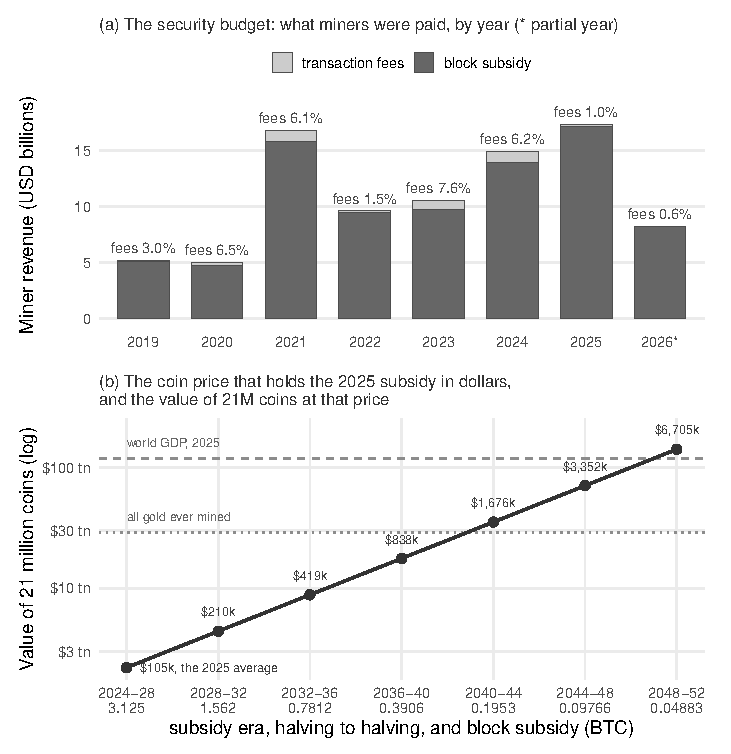
\includegraphics[width=\textwidth]{images/ch10_security_budget}
  \caption{(a)~The security budget by year: block subsidy and transaction fees paid to miners, in dollars, with the fee share. (b)~The price of one bitcoin that would hold the 2025 subsidy of \$17.2~billion constant in dollars through each coming halving, and the market value of 21~million coins at that price, against the value of all gold ever mined and a year of world output. Prices in the labels are per coin. Sources: miner revenue and fees, blockchain.com (daily, summed by year); world GDP, World Bank (2025); gold, World Gold Council (end-Q2 2026).} % fig-src: analysis/figures/fig_ch10_security_budget.R on analysis/data/ch10_security_budget_annual.csv and ch10_subsidy_schedule.csv (ch10_subsidy_arithmetic.R)
  \label{fig:outlook-budget}
\end{figure}

Table~\ref{tab:outlook-halving} does the sum. Hold the 2025 subsidy at its dollar value, \$17.2~billion a year, and ask what price each epoch's coins would have to fetch. The current epoch mints 164,250 coins a year, so the price is about \$105,000; the epoch that begins in 2028 mints half as many, so \$210,000; then \$419,000, \$838,000, \$1.7~million in 2040, \$3.4~million in 2044 and \$6.7~million in 2048. Multiply by 21~million coins. In 2040 the network would be worth \$35~trillion, more than every ounce of gold ever mined, which the World Gold Council valued at \$29~trillion in mid-2026. In 2048 it would be worth \$141~trillion, more than a year of the world's entire output, which the World Bank put at \$118~trillion for 2025 \autocite{worldbank2025gdp,wgc2026gold}. The gold comparison sets a stock against a stock; the output comparison sets a stock against a flow and is offered for scale, not as a limit, and both are in today's dollars against today's gold and today's output. % src: ch10_subsidy_arithmetic.R console (price for constant 2025 subsidy: 104,765 / 209,530 / 419,060 / 838,120 / 1,676,240 / 3,352,480 / 6,704,960; caps 2.2 / 4.4 / 8.8 / 17.6 / 35.2 / 70.4 / 140.8 $tn; gold $29.0 tn; GDP $118.35 tn)
The price of bitcoin can grow exponentially and has; what it cannot do is double every four years without end. Nor does a growing world economy rescue the path: output grew about 5~percent a year in dollars over 2023 to 2025, and on a price growing at that rate the dollar subsidy still falls by a factor of 0.61 every epoch, since a half times 1.05 to the fourth power is 0.61. With output growing at that rate the crossing moves from 2048 to about 2056, two halvings later, and does not disappear. % src: ch10_subsidy_arithmetic.R console (World Bank 2023 $107.35 tn to 2025 $118.35 tn = 5.0% a year; 0.5 x 1.05^4 = 0.61; constant-subsidy value of 21M coins exceeds growing world output from the 2056 epoch, 1.06x, against 2048 at fixed 2025 output)
No reader needs to decide what bitcoin is worth to see where this ends. A dollar subsidy held constant by price requires bitcoin to pass all the gold in the world within four halvings and a year of the world's output within six, or eight if the world keeps growing. My reading is that holding the subsidy constant in dollar terms becomes increasingly implausible beyond the 2030s under these assumptions.

\begin{table}[htb]
  \centering
  \scriptsize
  \setlength{\tabcolsep}{2pt}
  \begin{tabular}{lrrrrr}
    \hline
    \textbf{Epoch} & \textbf{Subsidy} & \textbf{Coins} & \textbf{Price to hold} & \textbf{21M coins} & \textbf{Fees to hold} \\
    from & BTC/block & per year & 2025's \$ & gold / GDP & 2025's \$, \$bn \\
    \hline
    Apr 2024 & 3.125 & 164,250 & 104,765 & 0.08 / 0.02 & 4.0 \\
    Apr 2028 & 1.5625 & 82,125 & 209,530 & 0.15 / 0.04 & 10.7 \\
    Apr 2032 & 0.78125 & 41,062 & 419,060 & 0.30 / 0.07 & 14.0 \\
    Apr 2036 & 0.39063 & 20,531 & 838,120 & 0.61 / 0.15 & 15.7 \\
    Apr 2040 & 0.19531 & 10,266 & 1,676,240 & 1.21 / 0.30 & 16.6 \\
    Apr 2044 & 0.09766 & 5,133 & 3,352,480 & 2.43 / 0.59 & 17.0 \\
    Apr 2048 & 0.04883 & 2,566 & 6,704,960 & 4.86 / 1.19 & 17.2 \\
    \hline
  \end{tabular}
  \caption{The halving schedule against a price path. Coins per year are 52,560 blocks times the subsidy; ``price to hold 2025's dollars'' is the 2025 subsidy revenue of \$17.2~billion divided by the epoch's coins; the next column values 21~million coins at that price against all gold ever mined (\$29.0~trillion, World Gold Council, end of the second quarter of 2026) and world GDP (\$118.35~trillion, World Bank, 2025). The last column is the fee revenue that would hold the 2025 security budget of \$17.4~billion with the price fixed at \$81,273, the price on September 4, 2026, at which the subsidy itself is worth \$13.4~billion a year in the current epoch, \$6.7~billion from 2028 and \$3.3~billion from 2032; 2025 fees were \$0.18~billion. Both bases run slightly high: 2025 ran about 53,100 blocks as hashrate grew, 1~percent more, and the revenue series behind the \$17.2~billion runs 2~percent above the coins issued times each day's price, so on 2025's own coins and prices the fourth and fifth columns would be about 3~percent lower, from \$101,700, every crossing in the same epoch, and each fee in the last column \$0.3~billion lower. Epoch dates after 2024 assume ten-minute blocks; subsidies are rounded to five decimals where needed.} % tab-src: analysis/data/ch10_subsidy_schedule.csv, written by analysis/checks/ch10_subsidy_arithmetic.R; basis lines of its console (2025: 53,082 blocks, 165,881 coins, 1.0% over 52,560; revenue-series subsidy $17.21 bn is 2.0% above coins issued x daily price, $16.87 bn; current-epoch price $101,705, 2.9% below $104,765; crossings on that basis gold 2040 at 1.18x, 2025 GDP 2048 at 1.15x, growing GDP 2056 at 1.03x; budget $17.05 bn, $0.34 bn below $17.38 bn, current-epoch fee $3.70 bn against $4.03 bn)
  \label{tab:outlook-halving}
\end{table}

The record so far has one epoch on each side of the doubling the table requires. Between the 2020 and 2024 halvings the price rose 7.3-fold, more than enough to grow the dollar subsidy through a halving; in the two years and four months since the 2024 halving it has risen 27~percent, less than the halving took away. % src: ch10_subsidy_arithmetic.R console (price $8,754 on 2020-05-11; $63,824 on 2024-04-20; $81,273 on 2026-09-04)
The subsidy in dollars fell from \$15.8~billion in 2021 to \$9.5~billion in 2022, and stood at \$17.2~billion in 2025 with half the coins per block. % src: ch10_subsidy_arithmetic.R console (subsidy revenue 2021 15.8, 2022 9.5, 2023 9.8, 2025 17.2 USD bn)
Hashprice tells the same story from the miner's chair: it fell six-fold from 2021 to 2025 while the price of bitcoin roughly doubled, because the coins per block halved once and the hashrate competing for them grew about six-fold. % src: chapter 4 and chapter 9 (hashprice $0.310 to $0.051 per TH-day); analysis/data/hashprice_daily_2021on.csv: mean hashrate 145 EH/s in 2021, 928 EH/s in 2025; mean price $47,386 in 2021, $101,682 in 2025 = 2.15x

So when does the subsidy become too low to finance the business? Mining is never too unprofitable to exist, because difficulty adjusts: when the dollar subsidy falls, the least efficient machines leave, hashrate falls, and the miners who remain earn the same subsidy over fewer hashes until the business clears again. What falls is not the existence of mining but its size, and its size is the network's security. If the price stays where it is, the dollar subsidy is \$6.7~billion a year from 2028, \$3.3~billion from 2032 and \$1.7~billion from 2036, and the hashrate the network can pay for shrinks with it, by whatever share machine efficiency does not recover. For fees to hold the 2025 budget instead, users of block space would have to pay \$10.7~billion a year from 2028 and \$14~billion from 2032, against \$0.18~billion in 2025: sixty to eighty times 2025's fee revenue. % src: ch10_subsidy_arithmetic.R console (subsidy at $81,273: 6.67 / 3.34 / 1.67 $bn; fees needed 10.71 / 14.05 $bn vs 0.175 $bn in 2025)
No year in the record of Figure~\ref{fig:outlook-budget}(a) has seen fees on that scale, which leaves the question of who else might pay.

\section{Who Pays for Security When the Subsidy Is Gone}
\label{sec:outlook-payers}

Three parties could fund the hashes that the subsidy no longer does. What follows is my reading of each, on a record that thins from the first to the third.

The first is the grid, and Section~\ref{sec:outlook-cheaper} is the offer on the table. As hashprice falls, the grid's payments for flexibility grow from a tenth of a mine's revenue toward the whole of its margin, and a site that could not cover its power and grid costs on mining alone covers them with its switch. This is real, and it is the subject of this book, but it has a ceiling that the same table shows. The grid pays for the hours a mine is off. At a quarter of the 2025 hashprice the flexible site cleared its power and grid charges by \$4~million where the never-pausing one fell \$11~million short, but it did so with the S19j~Pro off 69~percent of the year and the S21~XP 40~percent, and a machine that is off produces no hashes. % src: ch10_hashprice_sensitivity.R console (25% row: off 68.9% / 39.6%)
The grid can keep a fleet in business; it cannot keep it hashing. The size of the grid's contribution says the same thing from the other side. Chapter~9's site earned about \$101,000 of flexibility per megawatt-year in 2025; on the roughly 4,600~MW of mining demand ERCOT carried at its 2025 peak, that is about \$0.5~billion a year against a security budget of \$17.4~billion, under 3~percent, and even at a quarter of the 2025 hashprice, \$227,000 per megawatt-year, it is \$1.0~billion. Most of it is cost avoided rather than cash received: the strike and the power target lower the power bill, the window removes a charge, and only reserves put money in. % src: ch10_hashprice_sensitivity.R console, grid sizing ($100,920 and $227,393 per MW-yr x 4,600 MW = $0.46 bn and $1.05 bn, $1.046 bn unrounded, so $1.0 billion; $101,270 and $229,829, printed $230,000 and $1.1 billion, until 2026-10-03, when the ledgers booked distribution at $0.50 per MWh consumed; the older $100,604 / $228,928 in this comment did not reproduce and was corrected 2026-09-20); chapter 7 opening (potomac2026somercot pp. i, 31, ~4,600 MW, the 2025 peak of aggregate mining demand; both the per-MW-year value, flex value / 67.13 MW of site capacity, and the 4,600 MW are capacity bases); chapter 9 fig:stack-shape (reserves the only cash segment, 2022 and 2024 of the planned site)
This is still the most important development in the economics of mining since the industrial ASIC, and it is not a substitute for the subsidy.

The second party is the users of block space, through fees, and the arithmetic above says what they would have to pay.

The third party is the holders, and this is the chapter's third sum. A holder of bitcoin benefits from every hash whether or not they paid for it, which is the shape of a public good: everyone benefits, nobody is billed. Such a good can be paid for when one beneficiary is large enough that the benefit to itself covers the cost. Holders already pay, through dilution, about \$172~million a year for each percent of the supply they hold (Section~\ref{sec:outlook-budget}); the question the schedule forces is whether they will pay explicitly when issuance no longer collects it for them, the way the owner of a vault pays the guards. The record has two cases, and only one of them touches mining. Tether, the issuer of the largest dollar stablecoin, has invested in generation and mining since 2023, from a 241~MW renewable park in El Salvador to a proposal in April 2026 to vote its shares for mergers of Twenty One Capital with the bitcoin financial services company Strike and with Elektron Energy, a large mining platform; by August, Twenty One had dropped Strike and had no binding agreement with Elektron \autocite{tether2023volcano,tether2026twentyone,xxi2026q2}. % src: tether2023volcano (Volcano Energy, 241 MW, Metapan); tether2026twentyone (April 29, 2026, re-read 2026-09-27: Tether Investments "intends to vote its shares in favor of a proposed merger between XXI and Strike", and of the combined entities with Elektron Energy, "a large-scale Bitcoin mining platform"); xxi2026q2 (Form 10-Q filed 2026-08-11: "no longer pursuing the acquisition of Strike", announced July 21, 2026; Risk Factors: "Strike, a leading Bitcoin financial services company", re-read 2026-09-27; "no binding commitments or agreements with respect to the acquisition of Elektron"); the registrant's name is Twenty One Capital, Inc., with no hyphen
The United States established a Strategic Bitcoin Reserve by executive order in March 2025, capitalized with forfeited coins that ``shall not be sold,'' and directed its Treasury and Commerce departments to find budget-neutral ways of acquiring more; the order, which says nothing about mining, stood unamended in September 2026 \autocite{whitehouse2025sbr}. % src: whitehouse2025sbr sec. 3(a), 3(c), re-read 2026-09-27 (no "mining", "miner" or "mine" in the text); Federal Register API, 2026-09-27: EO 14233 (document 2025-03992) has no disposition or executive-order notes, and a term search for "Strategic Bitcoin Reserve" returns only the order itself
Neither is a central bank buying hashrate. What the record points at is a structure rather than an event: a large holder that funds mining is paying for the security of its own balance sheet, and a large holder that funds mining next to a grid that pays for the mine's flexibility is splitting the bill with the grid. The miner sells the switch to the grid and the hashes to the holder. Whether treasuries, sovereign or corporate, come to see the security budget as a cost of holding the asset is the open question. The arithmetic of Section~\ref{sec:outlook-halving} forces it within two halvings, and the parties with the most to lose from leaving it open are the ones with the most coins.

\section{What the Book Adds Up To}
\label{sec:outlook-close}

Chapter~2 described a grid as a huge, humming engine that must be balanced every second, and a mine as a load that can be balanced against it. Eight chapters later the claim can be stated exactly. A mine holds one asset the grid cannot buy from a gas plant or a battery: the freedom to change what it draws inside a quarter-hour and to hold the change for as long as the grid needs, an hour or a February week, at a cost the machines were built to bear. Chapter~4 priced the threshold at which a miner exercises that freedom, Chapter~5 built the loop that exercises it, and Chapter~6 found the contracts that leave the switch in the miner's hand. Chapters~7 and~8 found the markets and the tariffs that pay for it. Chapter~9 found that the whole, set as an operator could have set it in advance, was worth 9.0, 8.0 and 15.8~percent of a site's margin after power and grid charges in 2022, 2024 and 2025 and 23.0 and 29.5~percent of it in 2021 and 2023, where hindsight would have made the storm year 52.6~percent, and that a fence with a cheap price is worth having only when it is firm. % src: chapter 2 opening (humming engine; balanced every second); chapter 9 sec:stack-rule; analysis/checks/ch9_optimal_stack.R console, re-run 2026-10-03: PLANNED lines, flexibility over never pausing (23.0% in 2021, 9.0% in 2022, 29.5% in 2023, 8.0% in 2024, 15.8% in 2025), and the 2021 HINDSIGHT CEILING line (52.6%; 52.7% until 2026-10-03, when the ledgers booked distribution at $0.50 per MWh consumed); the same shares are plan_flex / never_total and hind_flex / never_total in analysis/data/ch9_optimal_stack.csv

This chapter added the direction of travel. As hashprice falls, flexibility becomes a larger share of mining revenue in the modeled cases. Halvings push in that direction; price, fees and network hashrate decide how far it goes. The grid a mine joins is one that has asked for flexible load in so many words and is filling up with firm compute that will need a flexible layer beside it. And, on my reading of the second sum, the subsidy that has paid for the network's security so far cannot be held in dollars past the 2030s without bitcoin passing all the gold in the world, which, if the price stays near where it is, puts the question of who pays for the hashes on the table within two halvings. The grid is one of the answers, and this book has spent its length measuring it. It is not the whole answer.

Three predictions, then, in the first person and dated to the April 2028 halving, each tied to a table this book's repository will recompute. I expect the S21 generation to be running the S19j~Pro's game by then, with the older fleet's strike under the mean price in most zones (Table~\ref{tab:outlook-sensitivity}); the peak layer gone for new large loads and the payment for flexibility settled on the five-minute price (Section~\ref{sec:outlook-grid}); and the fee share of the security budget still in single digits (Figure~\ref{fig:outlook-budget}). What would prove me wrong: a fee market that holds a tenth of the budget for a full year; a price path above the doubling staircase of Table~\ref{tab:outlook-halving} for two epochs running; a final 12CP rule that keeps a peak game for new large loads; or a first full RTC+B year in which reserve prices recover. On this reading each halving enlarges the grid resource: every epoch turns each fleet into the previous fleet's marginal machine, whose flexibility is the largest share of what it earns.

That is why the book has the title it has. Bitcoin mining is a grid resource because its flexibility is the product, and the product is real: measured on public data, paid for by a market that did not design it, and, on the arithmetic of Table~\ref{tab:outlook-sensitivity}, a larger share of what a mine earns the further hashprice falls. What the bitcoiner takes from the grid's side of the ledger is that the less a hash is worth, the more of what the machine earns comes from answering the grid. % src: tab:outlook-sensitivity, flexibility as a share of mining revenue 9.4 / 13.8 / 26.1 / 47.8 / 84.3% at 100 / 75 / 50 / 35 / 25% of the 2025 hashprice, 2025 prices held (analysis/data/ch10_hashprice_sensitivity.csv, written by analysis/checks/ch10_hashprice_sensitivity.R), the claim's only support; chapter 9's ledger shares (planned 23.0 / 9.0 / 29.5 / 8.0 / 15.8% of profit, 2021-2025) move with scarcity, not in a trend, so they are not cited for it
What the grid engineer takes from the miner's side is that the load that follows the price best is the one whose economics force it to. Neither side needs to believe in the other's asset for the arrangement to work. They only need to agree on the price of a quarter-hour, and that, in Texas, they already do.


\backmatter

\chapter*{Glossary}
\addcontentsline{toc}{chapter}{Glossary}
\markboth{Glossary}{}

This book is written for two trades at once, so a term that is obvious to
one reader is often new to the other. Every entry here is the book's own
usage, taken from the chapter that introduces it, and each term appears in
exactly one form throughout: where two words are commonly treated as
synonyms and this book does not, the entry says so. The numbers in the
entries restate figures the chapters give, and each is sourced where its
chapter gives it, not here.

% A5 measure is narrow and many entries carry long hyphenated compounds and
% parenthesised acronyms. Give TeX room to stretch rather than overrun.
\begingroup
\emergencystretch=3em
\hbadness=6000
\begin{description}[leftmargin=0pt,style=unboxed,itemsep=0.35em,parsep=0.15em]
\item[12CP (Twelve Coincident Peak)] \hypertarget{glossary:12cp}{}The commission's proposed replacement for 4CP: twelve monthly peaks, one for every month from October through September, each measured over a thirty-minute interval instead of fifteen. \emph{Proposed in the Texas Register on July 24, 2026, final rules required by December 31, 2026. Spreading the same annual charge over twelve peaks makes each worth about a third as much, roughly \$3,500 per megawatt at the Oncor floor instead of \$10,500. See 4CP, minimum billing demand.}
\item[2x16] \hypertarget{glossary:2x16}{}The sixteen daytime hours, 6 a.m. to 10 p.m. Central time, on Saturdays, Sundays and the six market holidays: every daytime hour that on-peak leaves out. \emph{The third of the three standard block products, with on-peak (5x16) and off-peak nights (7x8), and 1,760 hours in 2025. At LZ\_WEST that year the window averaged \$32 per megawatt-hour, the cheapest of the three, because it combines the solar belly with weak weekend demand. See block.}
\item[4CP (Four Coincident Peak)] \hypertarget{glossary:4cp}{}How ERCOT allocates transmission costs. In each summer month, June through September, ERCOT finds the single 15-minute interval of highest system-wide demand; a large consumer's share of the next year's transmission bill is then set by its average draw across exactly those four intervals. \emph{Demand here is a settlement quantity, not the raw control-room load: ERCOT sums metered generator output, nets off DC-tie flows and excludes grid-scale battery charging. It confirms each interval only after the month ends, so loads stay off across several candidate afternoons. Oncor's own share was about \$21,400 per megawatt of 4CP demand a year in 2025, and the ERCOT-wide charge a transmission-voltage site bears is roughly two to three times that, depending on the wires utility. The charge falls on peak megawatts, not on energy, so what avoidance is worth per megawatt-hour depends on the site: Chapter~6's ledger puts it at about \$5.65/MWh of the delivered price, at Oncor's transmission rate weighted over 2025 and a 95 percent capacity factor. Distinct from the summer window.}
\item[aggregator] \hypertarget{glossary:aggregator}{}A company that bundles many customers' curtailable load and fronts them to ERCOT through its own QSE, handling telemetry, offers, tests and settlement, and keeping a share of the proceeds. \emph{What it charges is a private commercial term: no aggregator publishes its revenue share, so this book prints none. The route costs a slice of the revenue and surrenders control of when the site is offered.}
\item[ancillary service (AS)] \hypertarget{glossary:ancillary-service}{}Insurance ERCOT buys alongside energy: standing capabilities that keep the lights on when something breaks. ERCOT's current set has five members; a sixth, the Dispatchable Reliability Reserve Service, is approved but not yet running, and only generators may sell it. \emph{Because ERCOT buys readiness, a load that can vanish in seconds is itself a sellable service. Since RTC+B every SCED run awards and prices all five; the Day-Ahead Market still clears them, now as financial positions.}
\item[Antminer S19j Pro (S19j Pro)] \hypertarget{glossary:antminer-s19j-pro}{}One of the book's two standing machines: a 2021-vintage workhorse that still populates mining farms in large numbers, 104~TH/s at 3,068 W, which is 29.5~J/TH. \emph{At the book's \$42.18 price anchor its breakeven hashprice is \$0.030 per terahash-day, a line the market crossed in 2026. At the 2025 mean hashprice its strike was \$72 and it paused 14 percent of the year: the machine that earns its keep by knowing when to stop.}
\item[Antminer S21 XP (S21 XP)] \hypertarget{glossary:antminer-s21-xp}{}The other of the book's two standing machines: the 2024 flagship of the same manufacturer, 270~TH/s at 3,645 W, which is 13.5~J/TH. \emph{At the same price anchor its breakeven hashprice is \$0.014 per terahash-day, below anything the market has recorded; at the 2025 mean hashprice its \$157 strike sat above almost every price the year produced. The 3,645 W is wall draw, not the PSU rating. It inherits the S19j~Pro's 2025 strike when hashprice falls to 46 percent of its 2025 level.}
\item[ASIC] \hypertarget{glossary:asic}{}An Application-Specific Integrated Circuit: a chip, and by extension the machine built around it, engineered for nothing but mining, capable of immense numbers of hashes per second at the cost of significant energy consumption. \emph{Replaced general-purpose computers in mining entirely by 2015. An ASIC cannot be repurposed for other computing work, which is why an idled mining machine is a load that can stop, not a data center that can switch tasks.}
\item[autotuning firmware] \hypertarget{glossary:autotuning-firmware}{}Miner firmware that retunes each hashing chip's voltage and frequency individually, so the machine can be held at any power level across a wide range rather than at the one operating point stock firmware ships with. The component doing the work is the autotuner. \emph{Per-chip retuning is why the autotuned fleet average beats the nameplate at stock power, 28.5 against 29.5~J/TH on the S19j~Pro. Moving to a power target with no saved tuning profile has a cost: the autotuner walks every chip to new settings, and the machine hashes below its optimum for the settling period of that tuning run. A target it already holds a profile for can be applied again without a new run, but only that exact target. After its first move away from stock power, the loop in Chapter~5's backtests applies only four targets on the S21~XP and eight on the S19j~Pro, so each needs one tuning run, barring a re-tune after a large change in chip temperature.}
\item[availability factor] \hypertarget{glossary:availability-factor}{}The share of an ERS load's committed quarter-hours in which it was actually available, which sets the availability component of its payment. A load consuming less than 95 percent of the capacity it contracted is counted unavailable for that interval, whatever the reason. \emph{Real deployments and tests are carved out; price response and peak-dodging are not. Only when a QSE's whole portfolio falls below 95 percent for the contract period can ERCOT suspend it and refer it to the commission. A summer afternoon block runs 255 obligated hours, so the 5 percent slack is under 13 hours.}
\item[backstop] \hypertarget{glossary:backstop}{}The rule that owns pause and resume. It reacts to accumulated damage rather than to a price merely crossing breakeven: while the price sits above the machine's breakeven at its most efficient power target within the loop's operating range the excess integrates, and the fleet pauses the moment the accumulated excess reaches \$10 per megawatt of load. The integral resets when the price dips back below breakeven, so a shallow blip never trips it, while a single five-minute print \$120 or more above breakeven does. \emph{Resuming is deliberately harder than pausing: the price must fall 10 percent below breakeven and hold 15 minutes, with minimum runtimes of 30 minutes each way and at most eight cycles a day. In thirty months of backtest across all eight ERCOT load zones it tripped 0.12 to 0.53 times a day. Modulation can never trigger a pause.}
\item[balancing authority] \hypertarget{glossary:balancing-authority}{}The grid operator responsible for watching the supply and demand balance in its area and adjusting generation output or shifting loads to keep the two in sync. \emph{The book's own term is grid operator; Chapter~2 gives balancing authority once, as the industry's name for the same role.}
\item[base point] \hypertarget{glossary:base-point}{}A target consumption level sent to a Controllable Load Resource by the same five-minute economic dispatch that steers every power plant in Texas, scored for compliance every interval. \emph{Not the site's own power target. The base point is the grid's instruction; the power target is how the site meets it.}
\item[basis] \hypertarget{glossary:basis}{}The gap between the trading hub price at which a futures block settles and the load zone price a mine actually pays. It is a risk the block does not cover. \emph{Not cost basis: this is a locational spread, not a purchase price. See hub, load zone, block.}
\item[behind the meter] \hypertarget{glossary:behind-the-meter}{}The trade's term for what ERCOT calls a Private Use Network: a mine built beside a generator and taking power across the fence, so that it stops being a retail customer of the grid. \emph{See Private Use Network for the definition and fence for what the deal pays and gives up.}
\item[Bitcoin block] \hypertarget{glossary:bitcoin-block}{}A batch of transactions proposed for addition to the Bitcoin blockchain. Miners repeatedly hash its data in search of a valid proof of work. Not the electricity contract called a block.
\item[black start] \hypertarget{glossary:black-start}{}Restarting a collapsed grid from a handful of designated units that can start with no outside power, typically hydroelectric plants or gas turbines with their own on-site generators. Most plants cannot start at all when the grid is dead, because they need grid electricity to run their own equipment. \emph{Operators use those units to energize pre-planned cranking paths, transmission corridors that carry station power to larger plants, which then start up, pick up a small block of customers and extend the electrified island outward; reconnect too much at once and cold-load pickup, the surge when every thermostat and compressor in a cold, dark city switches on together, collapses the young island's frequency again. This is why recovery takes days, not hours: ERCOT's leadership estimated a full black start in 2021 would have left most of the state dark for weeks.}
\item[block] \hypertarget{glossary:block}{}A fixed price bought for a fixed slice of the week, hedging some hours and leaving the rest exposed. Blocks have exact hour definitions because they trade as monthly futures, each settling against the average of the hub's settlement point prices inside its own window. \emph{Not a Bitcoin block: this is a power product, and the protocol's sense of the word is under block reward, block subsidy and block time. The three standard shapes tile the year with no gap and no overlap: on-peak (5x16), 2x16 and off-peak nights (7x8) were 4,080, 1,760 and 2,920 hours in 2025. A fourth quote, 7x24, is all of them at once. See basis.}
\item[Block Load Transfer (BLT)] \hypertarget{glossary:block-load-transfer}{}A group of customers disconnected from its usual grid area and connected to a neighboring one. \emph{The official peak calculation accounts for these transfers; the book's generation-based demand proxy does not separately reconstruct them.}
\item[block reward] \hypertarget{glossary:block-reward}{}What the miner who finds a valid block receives: newly minted bitcoins plus any transaction fees from the block it processed. This is the revenue that pays for the hardware and the electricity. \emph{The newly minted part alone is the block subsidy; the block reward is subsidy plus fees, and the book never uses one for the other.}
\item[block subsidy] \hypertarget{glossary:block-subsidy}{}The newly created bitcoin paid to the miner of each block, currently 3.125 bitcoin. With 144 blocks in an expected day that is 450 BTC a day paid out to the whole network, before transaction fees. \emph{The larger part of miner revenue, not the whole of it. It is not a price paid by any customer, and no miner can produce more of it.}
\item[block time] \hypertarget{glossary:block-time}{}The average interval between blocks, which the difficulty adjustment holds at roughly 10 minutes no matter how much hashrate the network has. \emph{The 10-minute target is the reference point for every difficulty claim in the book: during Winter Storm Fern average block times stretched to about 12.4 minutes.}
\item[breakeven price] \hypertarget{glossary:breakeven-price}{}The electricity price at which a machine's mining revenue exactly covers its power bill. Above it the machine mines at a loss and, sooner or later, shuts down. \emph{It is the mirror of efficiency at a given hashprice: when the block subsidy alone paid about \$0.032 per terahash-day, as in August 2026, a machine paying \$50 per megawatt-hour breaks even at about 27~J/TH and one paying \$40 at about 33~J/TH. Both move with hashprice. Chapter~4 derives the arithmetic; the same number used as a live tripwire is the strike price.}
\item[capacity market] \hypertarget{glossary:capacity-market}{}A second revenue stream, used in most U.S. markets but not in ERCOT, that pays a generator for simply existing and promising to be available years into the future. \emph{ERCOT has none, and that absence is what forces its scarcity prices to run so high.}
\item[capacity price] \hypertarget{glossary:capacity-price}{}The price of standby itself: dollars per megawatt for each hour an ancillary award is held, written \$/MW per hour, not dollars per megawatt-hour of energy. \emph{A resource earns it on its committed megawatts every hour it holds the award, on top of whatever it earns selling or consuming energy. Keep the capacity-price unit separate from the energy-price unit.}
\item[capture] \hypertarget{glossary:capture}{}The share of a perfect-foresight benchmark's gain that a real strategy earns over the same intervals, the gain being profit above running at stock power and never pausing. \emph{A percentage scored by a strategy, not a price: distinct from captured price, which is the dollars per megawatt-hour a generator's output actually fetched at its node. The shortfall is not all blindness: in Chapter~5's backtests, out of sample, the loop's own rules cost two-fifths to half of it. See oracle (perfect-foresight twin), captured price.}
\item[captured price] \hypertarget{glossary:captured-price}{}The average price a plant's output actually fetched at its own node. \emph{Across ERCOT in 2025 that was \$19 per megawatt-hour for wind and \$21 for solar, less than half the zone price a load pays. It is the floor of the behind-the-meter negotiation: below about \$19 the generator would rather sell to the grid, and above about \$40, priced on the same wind hours, the mine would rather buy those hours from the grid.}
\item[cascading failure] \hypertarget{glossary:cascading-failure}{}A chain reaction in which power from a failed line shifts onto neighboring lines, which overload and trip in turn, until generators and loads across a region fall out of sync. \emph{The 2003 Northeast blackout is the book's case for it.}
\item[the commission] \hypertarget{glossary:the-commission}{}The Public Utility Commission of Texas, the state regulator that sets the rules ERCOT operates under, approves its protocol changes and decides the transmission tariffs this book prices. \emph{It is the body behind the 4CP rule, its proposed 12CP replacement, and the Emergency Response Service. It also selects the market monitor and supervises it, while keeping every enforcement power in its own hands.}
\item[the companion repository] \hypertarget{glossary:the-companion-repository}{}The public code and data behind every number the book computes: each chapter's ledger scripts, the checks on them, and a historical calculator that runs the same engine for a different mix of the two machines, zone or contract. It is at \repourl.
\item[congestion cost] \hypertarget{glossary:congestion-cost}{}The second component of the LMP: what the transmission limits between a node and the rest of the grid add to or subtract from the System Lambda. \emph{When the system is uncongested prices are nearly uniform; when a line reaches its limit the grid splits into cheap and expensive regions and the LMPs say so. In ERCOT this is the only thing location does to a price, because losses are not priced into the LMP.}
\item[Controllable Load Resource (CLR)] \hypertarget{glossary:controllable-load-resource}{}A registration for loads that give ERCOT's dispatch engine direct control in exchange for fuller market participation. Some miners hold it. \emph{A 2024 rule change, approved but awaiting implementation, will move every CLR that is not an aggregation of small sites from zonal to nodal dispatch and settlement. A CLR is a load resource, the controllable form: do not confuse it with the basic form, which trips on an under-frequency relay or drops on a call. A CLR takes a base point, must respond to frequency at five percent droop (under a change ERCOT schedules for early 2027, only a CLR qualified for Regulation or Responsive Reserve), and is the only load registration that can sell Regulation.}
\item[curtailment] \hypertarget{glossary:curtailment}{}Output or load coming off the grid, whoever sets it off. For a load: the site acting on a price or its own rule, or ERCOT or a generator sending an instruction the site has agreed to follow. For a generator it is the mirror image, output held back because the grid cannot take it. This is the industry's word and the book uses it both ways. \emph{Where it matters that the machine stopped on its owner's rule rather than on somebody else's instruction, the book says pause. See pause, load shedding.}
\item[DART spread] \hypertarget{glossary:dart-spread}{}The difference between the day-ahead and real-time prices at the same place and hour. It is a market in itself: buy day-ahead and sell real-time, or the reverse. \emph{In 2024 the two markets differed by about \$17 per megawatt-hour on average in absolute terms.}
\item[Day-Ahead Market (DAM)] \hypertarget{glossary:day-ahead-market}{}A voluntary but financially binding forward market. Participants submit offers and bids for each hour of the following day, ERCOT clears energy and ancillary services together, and the hourly prices are published by 1:30 p.m. Central Time. \emph{A load pays the day-ahead price only for the volumes it actually bought there; whatever it consumes above or below that position settles at the real-time price.}
\item[DC tie] \hypertarget{glossary:dc-tie}{}The direct-current link over which ERCOT exchanges power with neighboring grids. \emph{Power flowing out over the ties is excluded from the settlement demand figure that sets 4CP, one reason the settlement peak and the live dashboard peak can name different quarter-hours; grid-battery charging is the other exclusion and the larger one. ERCOT's whole external connection is three DC ties and one variable-frequency transformer, about 1,220~MW.}
\item[demand response] \hypertarget{glossary:demand-response}{}Grid programs that pay an electricity consumer to stop consuming when the grid is short. A miner enrolled in one earns money from the grid instead of from mining during a price spike. \emph{Demand response is the program that pays for the curtailment, not the act itself. A machine the program's call turns off is curtailed; one its owner's own rule turns off is paused, the self-initiated kind of curtailment. See curtailment, pause.}
\item[demand-side reserve] \hypertarget{glossary:demand-side-reserve}{}A load that stands ready to stop consuming so that its unused power serves the rest of the system, giving the operator the same balancing effect as a reserve generator. A grid operator gets that effect by curtailing a batch of miners that has signed up for it. \emph{The book's one analogy for this is the demand-side battery, an analogy and not a second term, and an imperfect one, since a mine stores nothing and can only stop drawing.}
\item[development fee (devfee)] \hypertarget{glossary:development-fee}{}What Braiins~OS charges for its use, paid in hashrate rather than money: the firmware assigns a share of each machine's hashrate to Braiins Pool, the company's mining pool. \emph{2.5 percent on the two machines of Chapter~9. The ledger does not take it out, and it falls on all of a machine's hashing, not on the power-target layer alone.}
\item[difficulty] \hypertarget{glossary:difficulty}{}The protocol's self-balancing knob. The network automatically adjusts mining difficulty approximately every two weeks, every 2,016 blocks, so blocks keep arriving at the target rate: more hashrate raises difficulty, less hashrate lowers it. \emph{Hashrate and difficulty track each other almost perfectly, because added hashrate directly triggers added difficulty. Difficulty is a consequence of hashrate, not an independent input.}
\item[difficulty adjustment] \hypertarget{glossary:difficulty-adjustment}{}The protocol's two-week recalibration, which resets difficulty to whatever hashrate the network averaged over the previous 2,016 blocks and so restores the ten-minute block cadence at the next boundary. \emph{Winter Storm Fern was the test at scale: about 200~EH/s went offline at U.S.-facing pools, average block times stretched to about 12.4 minutes, the next adjustment was the largest downward move since China's 2021 mining ban, and the one after it rose 14.7 percent as the machines returned. Issuance is safe across it because coins are issued per block, not per minute. Sometimes called the retarget elsewhere; this book uses difficulty adjustment throughout.}
\item[Dispatchable Reliability Reserve Service] \hypertarget{glossary:dispatchable-reliability-reserve-service}{}A sixth ancillary service, approved in July 2026 and waiting on ERCOT's systems: generator capacity that must reach its level within two hours and hold it for four. \emph{Generators only, so a mine's load cannot sell it; only a plant the mine registers as a generation resource could. Its arrival cuts Non-Spin's endurance to two hours.}
\item[distribution] \hypertarget{glossary:distribution}{}The local delivery of power at lower voltages, after transformers step the voltage down, to neighborhoods, businesses and individual consumers. \emph{Large mining sites usually sit on the transmission or sub-transmission system, not on distribution.}
\item[droop] \hypertarget{glossary:droop}{}The standard slope that ties the size of a resource's frequency response to the size of the frequency error; ERCOT sets it at five percent wherever a Controllable Load Resource must answer frequency. \emph{Droop sets how hard a resource answers; the frequency deadband sets where it starts answering. See frequency deadband, Controllable Load Resource.}
\item[duck curve] \hypertarget{glossary:duck-curve}{}The shape of average price plotted against hour of day in a solar-heavy market: a deep belly at midday where solar floods the market and a steep neck in the evening when it withdraws. \emph{At LZ\_WEST in 2025 the midday hours averaged about \$21 and the evening ramp about \$72, more than three times as much a few hours apart on the same average day.}
\item[efficiency curve] \hypertarget{glossary:efficiency-curve}{}A machine's efficiency plotted across its whole power range instead of as a single number. Because autotuning firmware can hold a miner at any power level in that range, every power level has its own J/TH and the single operating point of stock firmware opens into a curve. \emph{The curves in this book are fleet averages of aggregated operating data from miners running Braiins~OS, second quarter of 2026, not laboratory curves. An individual machine sits somewhere around them, not on them.}
\item[efficiency (J/TH)] \hypertarget{glossary:efficiency}{}A mining machine's power draw divided by its hashrate, in joules per terahash. Lower is better. It is the single most important specification of a mining machine, because it sets the electricity price at which that machine stops being profitable. \emph{This is the one unit in the book where the good direction is down: 23.8~J/TH is more efficient than 29.5. Anchors: the Antminer S9 needed roughly 100~J/TH a decade ago, the S21~XP of 2024 needs 13.5, the latest hydro machines below 10, and this book puts the network's fleet average between 18 and 26~J/TH at the machines as of August 2026, with my own estimate at 21.5~J/TH; the listed fleets that publish their efficiency averaged 17~J/TH, weighted by hashrate.}
\item[Emergency Pricing Program (EPP)] \hypertarget{glossary:emergency-pricing-program}{}The circuit breaker added under the system-wide offer cap in December 2023: once real-time prices have been at \$5,000 per megawatt-hour for 12 hours within any 24, the cap on energy and ancillary-service offers falls to \$2,000 for at least a day and until a day after any emergency ends. \emph{Under it a week like Uri's could not recur at its price, so the values the book measures in that week were priced under 2021's rules. See system-wide offer cap, Winter Storm Uri.}
\item[Emergency Response Service (ERS)] \hypertarget{glossary:emergency-response-service}{}ERCOT's contracted reserve of last resort, deployed when operating reserves fall below 3,000~MW or an emergency is declared, that is, after the ancillary services of Chapter~7 have already been used. A load contracts months ahead to act on ERCOT's call and is paid for the promise whether or not the call ever comes. \emph{Budget capped by rule at \$75 million a year plus \$25 million for emergency renewals; procured four times a year in ten-minute and thirty-minute varieties with an offer cap of \$80 per megawatt per hour; deployment bounded at 24 cumulative hours in a winter contract period and 12 in the others; eleven deployments in eighteen years. It cleared at about \$4.36 per megawatt per hour on average in 2025 and \$18.69 in its summer-afternoon block, which collides directly with the peak layer (see ERS time period).}
\item[energy-only market] \hypertarget{glossary:energy-only-market}{}ERCOT's market design, in which a generator earns money by selling energy and ancillary services and nothing else. If those revenues do not justify building a plant, the plant does not get built. \emph{The design allows prices during scarcity to rise very high, which is exactly what makes the market pay for a load that can get out of the way.}
\item[energy storage resource (ESR)] \hypertarget{glossary:energy-storage-resource}{}ERCOT's name for a grid battery, the one asset class whose entire business is deleting price extremes: it buys the trough and sells the peak. \emph{Every megawatt of it lifts the floor and shaves the spike the miner's option was written on. A battery is duration-limited, about 1.8 hours average storage in 2025, and gives back about 85 percent of what it takes in, so it buys about 1.2 megawatt-hours for every one it sells; a pausing miner has no state of charge, owes no energy back, and can stay off for an hour or a week.}
\item[ERCOT] \hypertarget{glossary:ercot}{}The Electric Reliability Council of Texas, operator of the Texas Interconnection and the market this book is about. It serves about 90 percent of Texas electric load and more than 27 million customers, and because its wires stay almost entirely inside Texas its wholesale market is exempt from FERC rate regulation. \emph{Federal reliability standards still apply through NERC; only wholesale rate regulation is exempt. More Bitcoin mining load is connected here than anywhere else in the world.}
\item[ERCOT Contingency Reserve Service (ECRS)] \hypertarget{glossary:ercot-contingency-reserve-service}{}The ten-minute reserve: capacity ERCOT can call to restore the crash barrier after it has been used, sustained for at least an hour (two hours until RTC+B cut it in December 2025). Launched June 10, 2023, the first new daily procured service in more than twenty years. \emph{Its first year is the book's cautionary case: the market monitor found that the way ECRS was procured and withheld created artificial shortage pricing and added more than \$12 billion of real-time market costs, for a computed reliability benefit of about \$12 million against more than \$600 million of procurement cost. It is the product at the center of the reserves-or-strike trade-off in Chapter~9.}
\item[ERS time period] \hypertarget{glossary:ers-time-period}{}The standing block of hours a load sells into ERS and must stay available for the whole contract term. There are eight: five weekday daytime and evening blocks, two for weekends and holidays, and one for everything left over. \emph{The fourth block is weekdays from 4 to 7 in the afternoon, and 29 of the 32 official 4CP intervals fall inside it, which is why a mine that intends to dodge the peak should never sell that block.}
\item[failure to provide] \hypertarget{glossary:failure-to-provide}{}Under the pre-December 2025 rules, what happened when a committed load stopped consuming: the reserve it had sold vanished, ERCOT bought replacement capacity, and the seller was billed at replacement cost. \emph{Pausing during a \$3,000 spike, the move Chapters~5 and 6 spend forty pages perfecting, was a failure to provide. The charges and the replacement-procurement market were deleted from the rulebook at RTC+B go-live. The two-failure rule still stands: two failures in a rolling year to answer a deployment disqualify a relay-only load, with a six-month wait to reapply. It counts missed deployments, not pauses as such, and it never applied to a CLR.}
\item[fast frequency response (FFR)] \hypertarget{glossary:fast-frequency-response}{}The fastest sub-form of Responsive Reserve, supplied almost entirely by batteries but open to any resource fast enough, a load included: full output within a quarter second of a frequency trigger, sustained at least fifteen minutes. \emph{FFR and the loads' under-frequency relay share one cap: together they may cover no more than 60 percent of the RRS requirement.}
\item[fence (the fence)] \hypertarget{glossary:fence}{}The book's shorthand for a mine behind the meter and for the deal that comes with it, as in Chapter~9's ``The Other Offer: Behind the Fence''. The fenced site pays one negotiated price per megawatt-hour and nothing else: no losses, no ancillary or uplift allocation, no distribution line, no transmission charge. \emph{It also sells no reserves, dodges no peaks and arbitrages no index. The fence is an annuity; the stack is an option. See Private Use Network, indifference price, hybrid.}
\item[FERC (Federal Energy Regulatory Commission)] \hypertarget{glossary:ferc}{}The U.S. regulator of interstate electricity transmission and wholesale sales. See NERC for the organization that develops and enforces bulk power system reliability standards.
\item[firm load] \hypertarget{glossary:firm-load}{}A load contracted to run whatever the price does. Today's AI campus is built and contracted as one, because nobody pauses a training run for a price. \emph{The opposite of the flexible layer beside it: in Winter Storm Fern ERCOT credited about 4,100~MW of curtailment to miners against about 170~MW to data centers. Not the same use of ``firm'' as firm supply, which is a duty on the generator.}
\item[firm supply] \hypertarget{glossary:firm-supply}{}A behind-the-meter deal in which the generator must keep the power flowing, so the mine runs whenever it wants. \emph{The firm case is a ceiling for the fence: an always-available plant is the most favorable assumption the ledger makes for it. Contrast interruptible.}
\item[flexibility] \hypertarget{glossary:flexibility}{}The product a mine sells to the grid: the freedom to change how much power it draws inside a quarter-hour, on a price signal, a demand signal or a dispatch instruction, at a cost the machines were built to bear. \emph{In the ledger the word also names a quantity: the planned site's margin over the never-pausing site's, worth 9.0, 8.0 and 15.8 percent of the never-pausing margin in 2022, 2024 and 2025 and 23.0 and 29.5 percent in 2021 and 2023, the storm year and ECRS's first year. The best annual choice in hindsight would have made the storm year 52.6 percent; see hindsight ceiling. Every such margin is after power and grid charges; see never-pausing site.}
\item[the flexibility stack (the stack)] \hypertarget{glossary:the-flexibility-stack}{}The layers a site runs at once to earn from flexibility: the strike, the power target and the summer window, with reserves beside them. They are not additive, because a megawatt does one thing in one quarter-hour. \emph{Chapter~9's own correction to its title: the strategy is not a stack but an order of switching. Inside the year it runs with no look-ahead at all; its two annual switches, reserves and the summer window, are the only choices the ledger could have made with hindsight, and its headline sets them in advance (see planned site, hindsight ceiling). On my reading, under RTC+B and, if it is adopted as proposed, 12CP, the stack collapses toward one layer, the moving strike with the power target beside it, and falling hashprice makes that layer thicker.}
\item[flexible load] \hypertarget{glossary:flexible-load}{}A load that can rapidly scale down or shut off its power usage when the grid needs it to. Bitcoin mining is the book's central example. \emph{ERCOT's Winter Storm Fern accounting put roughly 4,100~MW of the January 2026 reduction on cryptocurrency miners, second only to the oil and gas sector and more than twenty times what conventional data centers contributed.}
\item[frequency deadband] \hypertarget{glossary:frequency-deadband}{}The band of frequency error inside which no response is demanded. A Controllable Load Resource's may be no wider than plus or minus 0.036~Hz against a 60.000-hertz target, so outside that band it must answer like a power plant's governor (under a change ERCOT schedules for early 2027, only if it is qualified for Regulation or Responsive Reserve). \emph{Not the price deadband of Chapter~5, which is a band of dollars, not hertz. See droop, Controllable Load Resource, price deadband.}
\item[generation resource] \hypertarget{glossary:generation-resource}{}The full ERCOT resource class, which may offer energy, be committed and dispatched, and sell ancillary services. In exchange it takes on continuous telemetry, a standing offer whenever it is online, and the duty to run when ERCOT commits it for reliability. \emph{The counterpart to a Settlement Only Generator; the choice between the two is the gate that matters for a miner who owns a plant.}
\item[halving] \hypertarget{glossary:halving}{}The scheduled event, about every four years, that cuts the block subsidy in half and so reduces the issuance rate of new bitcoins. \emph{Four so far: 2012, 2016, 2020, 2024. The stretch between two of them is a halving epoch, the book's only sense of the word epoch.}
\item[halving epoch] \hypertarget{glossary:halving-epoch}{}The stretch between two halvings, about four years, across which the block subsidy is constant. \emph{In this book epoch always means a halving epoch. The protocol's other recurring interval, the two-week window between difficulty adjustments, is called a difficulty period here and never an epoch. See halving, difficulty adjustment.}
\item[hashprice] \hypertarget{glossary:hashprice}{}The dollars a unit of hashrate earns per day: network revenue per day, subsidy plus fees, times the bitcoin price, divided by the network hashrate. The book quotes it in dollars per terahash-day (\$/TH/day), a terahash-day being one terahash per second of hashrate sustained for a day. \emph{Three principal drivers shape it: the bitcoin price, the network hashrate and the scheduled halving. The book's anchor year is 2025, which averaged about \$0.051 per terahash-day. Watch the units: market convention also uses \$/PH/day, a thousand times larger.}
\item[hashrate] \hypertarget{glossary:hashrate}{}The computational power a miner or the whole network brings to the puzzle, measured in hashes per second: terahashes per second (TH/s) for a machine, exahashes per second (EH/s) for the network. \emph{Network hashrate is about 930~EH/s as of August 2026, down from a peak of roughly 1,100~EH/s in late 2025.}
\item[hindsight ceiling] \hypertarget{glossary:hindsight-ceiling}{}The best annual choice in hindsight: the site runs on whichever reserve allocation, product and summer-window call scored best on the year's own outcomes. \emph{The oracle's discipline applied one level up, to the annual switches; inside the year it still runs the lagged loop. Printed beside the planned site and never called a strategy, because it needs the year's prices before the year starts; in 2021 it needs to know in January that Uri is coming. Its flexibility was 52.6 percent of the never-pausing margin in 2021 and \$233 million over the five years, against the planned site's 23.0 percent and \$123 million.}
\item[hosting agreement] \hypertarget{glossary:hosting-agreement}{}The contract under which a site's owner, the host, runs a tenant's machines on its power. It decides who holds the right to curtail. \emph{In the public Rockdale agreements of Chapter~6 the host holds it: one has the host sell the power instead once the ERCOT market's profitability passes a redacted share of the contract price, the other lets it enroll the site in any demand response program at its sole discretion, and each passes part of that value back to the tenant. The book's site is an owner-operator's, which buys its own power and holds that right itself.}
\item[hub] \hypertarget{glossary:hub}{}A trading settlement point whose price averages the LMPs of a fixed list of major 345 kV buses. Traders hedge at hubs (North, South, West, Houston and a few others), and hub prices anchor most financial contracts. \emph{A hub is a financial construct, not a place a load can be billed at; a consumer still pays its load zone, and the gap between the two is the basis.}
\item[hybrid] \hypertarget{glossary:hybrid}{}A site that sits behind a generator and in front of the grid at once, keeping both the fence's discount and its own switch. \emph{The hybrid buys the annuity and keeps the option. The book describes it but does not model it, because the companion repository holds no generator-availability data. Hut 8's Vega runs behind a wind farm and in front of the grid at once. Not a generator co-located with a battery, which the trade press also calls a hybrid.}
\item[hydro] \hypertarget{glossary:hydro}{}Shorthand for a liquid-cooled mining machine. Hydro models sit at the efficiency frontier, with the latest pushing below 10~J/TH. \emph{Not hydroelectric power. In mining, hydro describes how the machine is cooled, not where its electricity came from; Chapter~1 mentions hydroelectric dams in Canada, which is the other sense.}
\item[ICCP] \hypertarget{glossary:iccp}{}The grid world's standard control-room protocol: the language a QSE's control system uses to speak to ERCOT across ERCOT's own private wide-area network, on routers ERCOT supplies and manages at the QSE's premises. \emph{ERCOT's side of the private-network hookup is capped at \$7,000 to install and \$450 a month to run.}
\item[Independent System Operator (ISO)] \hypertarget{glossary:independent-system-operator}{}A neutral operator that runs the transmission system and the wholesale market on top of it. ISOs and RTOs own no generation and serve no retail customers: they dispatch generators, operate the transmission system and run the auctions where electricity is bought and sold. \emph{Roughly two-thirds of U.S. electricity consumers live in an ISO or RTO region; seven such markets serve them, and ERCOT is one. The book uses ISO and RTO for the same kind of institution.}
\item[index contract] \hypertarget{glossary:index-contract}{}A power contract under which the buyer pays the market's settlement price for every interval it consumes. The buyer carries all of the price risk. \emph{Texas banned wholesale-indexed products for residential and small commercial customers after Uri and left them fully legal for large loads. If you index, index real time (see real-time index).}
\item[indifference price] \hypertarget{glossary:indifference-price}{}The negotiated behind-the-meter price at which the fenced site earns exactly what the grid site earns. Below it the fence wins, above it the grid does. \emph{Quoted against three grid sites and the answers differ: against the planned site it was \$55, \$63, \$43, \$41 and \$44 from 2021 to 2025; against the hindsight ceiling it had no positive answer in 2021; against the never-pausing site it was \$192, \$84, \$76, \$50 and \$56.}
\item[inertia] \hypertarget{glossary:inertia}{}The energy stored in the spinning mass of every synchronous generator locked in step with the grid, which the grid draws on in the first seconds after a plant trips. It slows the fall of frequency; it cannot stop it. ERCOT's typically runs between 200 and 400 gigawatt-seconds, against a floor of 100. \emph{On ERCOT's accounting, wind, solar and batteries, which reach the grid through inverters, add none. During Uri's frequency emergency it stayed between 254 and 349 gigawatt-seconds: that night's danger was a shortage of reserves, not of inertia.}
\item[interconnection] \hypertarget{glossary:interconnection}{}A vast region whose generators all run synchronously at the same electrical frequency, 60~Hz in the United States, so power can flow across regional lines as needed. North America has the Eastern, Western and Texas interconnections. \emph{Texas is its own interconnection, which is why ERCOT can neither lean on nor be dragged down by its neighbors the way the Eastern Interconnection spread the 2003 cascade.}
\item[interference] \hypertarget{glossary:interference}{}How far the stack falls short of adding its layers separately: the joint price-only result less the naive sum of strike, power target and the whole transmission prize, negative in every year. \emph{The overstatement was 15 percent in 2025 and 34 percent in 2024, when two of the four peaks also escaped the summer window; in dollars it was largest in the storm year, because the strike was highest then. It exists because a megawatt does one thing in one quarter-hour.}
\item[interruptible] \hypertarget{glossary:interruptible}{}A behind-the-meter deal in which the generator keeps the right to take the power back and sell it to the grid, paying the mine nothing for the interruption. \emph{An interruptible fence matches the planned site at no price in any of the five years. Firmness matters alongside price in a behind-the-meter deal. Distinct from interruptible load, which is a property of the load, not a contract term.}
\item[interruptible load] \hypertarget{glossary:interruptible-load}{}A load that can be stopped for hours without ruining a product or inconveniencing anyone. Stopping a miner only delays hashing, which is why mining is interruptible by design. \emph{Distinct from interruptible, which is a contract term of Chapter~9, not a property of the load.}
\item[islanded] \hypertarget{glossary:islanded}{}Running with no grid tie at all. An islanded mine avoids every non-energy charge and loses the whole flexibility stack with it. \emph{It has no load zone price to arbitrage, cannot sell reserves, has no transmission peak to dodge and cannot enroll in the emergency-response programs. Distinct from a netted site, which keeps a grid tie and with it part of the flexibility stack.}
\item[Large Computational Load] \hypertarget{glossary:large-computational-load}{}A Large Load where half or more of the demand is computational load, such as data centers and cryptocurrency mining facilities. \emph{This is the term the commission's transmission reform asks about by name.}
\item[Large Load] \hypertarget{glossary:large-load}{}ERCOT's name for a load of 75~MW or more at a single site. It must complete ERCOT's large-load interconnection process, with system studies and a separate approval to energize, before it may draw power. \emph{By the end of 2025 ERCOT's large-load program, which takes loads of every industry, had about 5,800~MW energized, each site counted at its highest draw. By March 2026 over 9,000~MW, including those, held approval to energize; mining demand alone peaked near 4,600~MW in 2025 (Chapter~7). The 75~MW line is also where the proposed large-load demand management service would apply and, for a load that connects or expands under the commission's new interconnection rule, the proposed minimum billing demand.}
\item[large-load demand management service] \hypertarget{glossary:large-load-demand-management-service}{}The emergency product Senate Bill 6 adds alongside ERS, for sites of 75~MW or more called with 24 hours' notice. It bars any load that already curtails on price or sells another reliability or ancillary service, so it is written for the loads that do not already respond. \emph{The rule is still a proposal, which the commission's staff plans to bring for adoption in January 2027, so the service is not yet running; the proposal caps offers at \$5,000 per megawatt-hour and extends the exclusions to ERS and the utility programs.}
\item[load] \hypertarget{glossary:load}{}The electricity being consumed by end users at any given moment. The book uses load and demand for the same thing. \emph{A mining site is a load, never a generator, even when switching it off has the same balancing effect as adding supply.}
\item[Load Frequency Control (LFC)] \hypertarget{glossary:load-frequency-control}{}ERCOT's name for automatic generation control (AGC): the control-room system that, in the minutes after primary frequency response has stopped a fall, moves the generators and controllable loads selling Regulation until frequency is back at 60~Hz, sending a correction signal every four seconds. \emph{It brings frequency home; primary response only stops it falling.}
\item[load resource] \hypertarget{glossary:load-resource}{}A load registered with ERCOT to sell ancillary services. In its basic form it is wired to trip offline within half a second on an under-frequency relay, or curtailed on ERCOT's instruction, and paid for it. The ability to disconnect quickly is itself a sellable service. \emph{The Controllable Load Resource is the other form of the same registration: instead of tripping or dropping on a call, it follows a base point.}
\item[load shedding (firm load shed)] \hypertarget{glossary:load-shedding}{}The grid operator deliberately cutting power to blocks of customers, in rolling blackouts, to force supply and demand back into balance and save the rest of the system. ERCOT's and Senate Bill 6's name for it is firm load shed. \emph{Reserved for involuntary outages ordered by the operator (the automatic form, set off by relays with no order, is under-frequency load shedding): never a substitute word for curtailment, and never for a miner's pause. Customers who are shed do not choose and are not paid. During Uri, 1,000~MW was ordered at 1:20 a.m., 5,000~MW by 1:50, 8,500~MW by 1:55 and a maximum of 20,000~MW later that day. Under SB 6 any transmission-connected load interconnected after 2025, other than critical-load industrial customers and critical natural gas facilities, must be curtailable during it, under a protocol its wires utility puts in place before the load connects; the duty is written into the statute but not yet into a commission rule.}
\item[load zone] \hypertarget{glossary:load-zone}{}The settlement point a consumer pays: an average over every bus in the zone, weighted by how much load each bus is carrying. ERCOT defines eight, the four large competitive zones plus four belonging to utilities that did not open to retail competition (Austin Energy, CPS Energy, LCRA and Rayburn). \emph{Zones are sets of electrical buses, not geographic borders. Until nodal settlement for Controllable Load Resources switches on, every consumer's energy is billed at the zonal price.}
\item[Locational Marginal Price (LMP)] \hypertarget{glossary:locational-marginal-price}{}The cost of delivering one more megawatt-hour at exactly one node, computed by SCED roughly every five minutes at every node in the network model, and in the DAM once a day for each hour of the next operating day. In ERCOT it has two components only: the System Lambda plus the Congestion Cost. \emph{Unlike PJM, MISO and the other nodal markets, ERCOT's LMP has no loss component. Losses are recovered by scaling metered consumption up by a loss factor, so a site's location changes its price only through congestion, not through distance from the plants.}
\item[the loop] \hypertarget{glossary:the-loop}{}The book's name for the price-response layer of Chapter~5: it reads each new print, recomputes the profit-optimal power target, and applies the hold, the price deadband and the backstop. It owns both decisions a fleet makes on price, but never in one rule: modulation sets the power target, the backstop owns pause and resume, and the two read the same feed without sharing a decision. \emph{An abstraction on purpose, so the design can be argued on its own terms rather than any one vendor's. Braiins Manager's Price Adapt implements the loop (Chapter~5). Below the loop sits the autotuning firmware, which holds whatever target the loop asks for unless temperature safety forces it lower. See modulation, backstop, power target, autotuning firmware.}
\item[LZ\_WEST] \hypertarget{glossary:lz-west}{}ERCOT's West load zone, the one that appears throughout this book. West Texas has the state's best wind and solar resources, limited transmission out and much of the state's Bitcoin mining, which gives it the most volatile prices in ERCOT. \emph{Its 2025 average 15-minute real-time settlement point price, \$42.18 per megawatt-hour, is the book's price anchor.}
\item[marginal machine] \hypertarget{glossary:marginal-machine}{}The least efficient machine still running on the network at a given hashprice. Because the fleet lives on the breakeven line by construction, the marginal machine mines for nearly nothing, and its only remaining edge is the price it pays for power. \emph{Defined by the market, not by a model: it is whichever machine sits at the breakeven line today. This is why only the cost side decides who survives.}
\item[market monitor] \hypertarget{glossary:market-monitor}{}Potomac Economics, the independent firm that watches ERCOT's wholesale market for market power and design flaws and reports what it finds to the commission. The commission selects and supervises it, and ERCOT funds it out of the system administration fee that pays for ERCOT itself. It holds no enforcement power: statute reserves all of that to the commission. \emph{Statute and rule call it the independent market monitor, or IMM. Its annual State of the Market report is a standing source here, behind the ECRS verdict of Chapter~7 and the 4CP criticism of Chapter~8; the bibliography lists it under Potomac Economics.}
\item[mean reversion] \hypertarget{glossary:mean-reversion}{}The tendency of five-minute prices to fall back after a large upward leap rather than keep climbing; after a large fall they usually keep falling, as a spike unwinds over several prints. The level, not the trend, carries the information. \emph{At LZ\_WEST, from 2024 to mid-2026, the correlation between one five-minute price change and the next is about -0.29, and the spikes carry it: each of the five largest leaps, all of more than \$4,000, fell straight back at the very next print, while ordinary moves of a few dollars carry almost no signal either way, and the first half of 2026, when no print leapt that far, came out near zero. This is the structural reason there is no forecast in the loop: extrapolating a trend points the decision the wrong way, and it is most wrong during spikes, when the stakes are highest.}
\item[minimum billing demand] \hypertarget{glossary:minimum-billing-demand}{}Under the proposed rule, the demand billed whether or not the site consumes, for a load the commission's new large-load interconnection rule covers: a new site of 75~MW or more, or the added load of an expansion that first takes a site to 75~MW or adds 75~MW or more to one already past it. It is the greater of the peak demand written into its service contract, its highest demand in the past year, or its 12CP demand, billed for at least twenty years. \emph{As proposed, for such a load this ends peak avoidance altogether: transmission becomes a fixed cost. A site already energized when that rule takes effect on October 8, 2026, and not expanding, is outside it as proposed. The chairman of the commission called it a minimum demand ratchet.}
\item[mining pool] \hypertarget{glossary:mining-pool}{}A service that combines miners' computing power and shares the proceeds.
\item[modulation] \hypertarget{glossary:modulation}{}The gradual repricing of a running machine: moving its power target up and down the efficiency curve as the electricity price changes. \emph{Modulation never pauses or resumes anything; the backstop owns that. The two read the same price feed and never share a decision, which keeps noise out of the pause and resume path.}
\item[modulation floor] \hypertarget{glossary:modulation-floor}{}The lowest power target modulation will set: Braiins~OS's default minimum, or the machine's best-efficiency point where that is higher, since below the best point slowing further surrenders more hashrate than the electricity it saves. In this book, 1,200 W for the S19j~Pro and 2,774 W for the S21~XP. \emph{Past the floor there is only one move left, the full pause, and that decision belongs to the backstop. The loop clamps every computed target between this floor and the power ceiling.}
\item[negative price] \hypertarget{glossary:negative-price}{}An hour in which generators pay consumers to take power, because subsidized renewables can profitably produce below zero and shutting down costs them more. In West Texas it happens when renewable output exceeds what the wires can carry away. \emph{At a generator's own node the real-time price has a floor of -\$251/MWh. At LZ\_WEST in 2025 prices were negative 5.6 percent of the time.}
\begin{samepage}
\item[NERC (North American Electric Reliability Corporation)] \hypertarget{glossary:nerc}{}The organization that develops and enforces reliability standards for the North American bulk power system. See FERC.\par
\end{samepage}
\item[net load] \hypertarget{glossary:net-load}{}Demand minus wind and solar output. Its highest hour, the net-load peak, is the hour the system is actually short of power. \emph{ERCOT put the net-load peak at hour ending 21 in 2023 and 2024 and hour ending 22 in June and July 2025: the tightest hours of the day have migrated from the traditional four-to-five-p.m. demand peak to the seven-to-nine-p.m. net-load peak, the hour solar leaves. Not the 4CP interval, which counts gross demand with solar still shining and has stayed at 5 p.m.; ERCOT told its board in 2026 that 4CP does not correspond to the system's highest net-load peaks.}
\item[netting] \hypertarget{glossary:netting}{}Settling one number at the interconnection point in every quarter-hour, generation minus load. Net export settles as generation, net consumption settles as load and carries the load-side charges, and consumption that never crosses the meter is invisible to settlement. \emph{ERCOT forbids netting by default and allows it in five enumerated site configurations. Since Senate Bill 6, a load of 75~MW or more that seeks a new or expanded connection and nets against a plant already registered as stand-alone on September 1, 2025 needs the commission's approval first, on a 120-day ERCOT study and a decision 60 days after that, approved by default if the deadline passes.}
\item[never-pausing site] \hypertarget{glossary:never-pausing-site}{}The comparator site: the same fleet running at stock power in every interval, present at all four summer peaks, and paying every grid charge in full. Every gain in the ledger is measured against it. \emph{A baseline, not a strategy, and the denominator of the flexibility percentages. Its figure is a margin after power and grid charges; machines, depreciation, pool and firmware fees, site operation, staff and debt are outside the ledger.}
\item[node] \hypertarget{glossary:node}{}A physical junction where equipment connects to the high-voltage grid, such as a plant's switchyard or a substation where lines meet and transformers step the voltage down. The power network calls it a bus; the market calls it a node, and a large mine's own interconnection point is one. \emph{Bus and node are the same thing under two names; a node is a real place with coordinates, not a zone or a region. Not a Bitcoin network node, which is a computer running the protocol.}
\item[Non-Spinning Reserve (Non-Spin)] \hypertarget{glossary:non-spinning-reserve}{}ERCOT's slow reserve: capacity that can come online within thirty minutes, with four hours of endurance (two hours once the Dispatchable Reliability Reserve Service is running), the service that covers a forecast bust rather than an instant failure. \emph{The only product whose standing revenue was firming rather than falling at the 2026 run rate.}
\item[off-peak nights (7x8)] \hypertarget{glossary:off-peak-nights}{}The eight hours outside the daytime block, midnight to 6 a.m. and 10 p.m. to midnight, every day of the week, weekends and holidays included. \emph{One of the three standard block products, and 2,920 hours in 2025. At LZ\_WEST that year the window averaged \$49 per megawatt-hour and held firm while the daytime window sagged, because it is the one window solar never reaches. The trade also says off-peak for everything outside 5x16, which is 7x8 and 2x16 together; this book always means the nights. See block.}
\item[off share] \hypertarget{glossary:off-share}{}The share of quarter-hours in which a fleet draws nothing under the price-only stack, where the power target underclocks the machines before anything stops. \emph{Not the pause share. The S19j~Pro that paused 14 percent of 2025 under the plain strike rule drew nothing in only 7 percent of quarter-hours under the stack, because the engine underclocks first.}
\item[on-peak (5x16)] \hypertarget{glossary:on-peak}{}The sixteen hours from 6 a.m. to 10 p.m. Central time, Monday through Friday, excluding six market holidays. The market labels each hour by when it ends, so the window runs HE 7 through HE 22. \emph{One of the three standard block products, and 4,080 hours in 2025. At LZ\_WEST that year the window averaged \$41 per megawatt-hour, cheaper than the \$49 nights, because it now contains the solar belly. See block, 2x16, off-peak nights (7x8).}
\item[operating leverage] \hypertarget{glossary:operating-leverage}{}The sensitivity of a machine's margin to a move in hashprice, which grows as the share of revenue spent on electricity grows. \emph{On the eve of the August 2026 rally, at the \$42.18 price anchor, the S19j~Pro was spending 96 cents of every revenue dollar on electricity and the S21~XP about 44, so a ten percent move in hashprice barely registers at the efficient machine and doubles or erases the inefficient one's entire margin. Efficiency raises profits and reduces exposure to hashprice.}
\item[Operating Reserve Demand Curve (ORDC)] \hypertarget{glossary:operating-reserve-demand-curve}{}ERCOT's administered scarcity pricing mechanism from 2014 until the 2025 redesign: a real-time adder to the energy price that grows as available reserves shrink, reflecting the rising probability of losing load. When reserves were plentiful the adder was near zero. \emph{RTC+B retired the adder on December 5, 2025: shortage value now sits inside the energy price rather than being added to it afterwards, and only the curve's shape survives, in the ancillary-service demand curves cut from it.}
\item[operating reserves] \hypertarget{glossary:operating-reserves}{}The grid's safety margin, capacity held back and ready rather than producing. \emph{Valuable even in hours when no shortage materializes, which is why ERCOT pays for it administratively. Chapter~2 introduces the concept; Chapter~3 prices it.}
\item[optimal site] \hypertarget{glossary:optimal-site}{}Not a term of this ledger. Chapter~9 prints the planned site as its headline and the hindsight ceiling beside it; neither is optimal for a site that cannot see the year ahead. \emph{Chapter~10's sensitivity rows, which rerun 2025 alone, use the phrase for the price-only stack with the summer window played where it pays, which in 2025 is also the planned site. See planned site, hindsight ceiling.}
\item[oracle (perfect-foresight twin)] \hypertarget{glossary:oracle}{}The benchmark the loop is graded against: a hypothetical operator with perfect foresight and zero friction. In every interval it sets the machine to the profit-optimal power for that interval's own settlement price, which no one can know until the interval has ended, and it pauses for free whenever even that optimum would lose money. No hold, no price deadband, no minimum runtimes, no resume ramp, no publication delay. \emph{A ceiling on what responding to the energy price can earn, not a strategy; nothing real sees the future. Not a price oracle in the crypto sense: nothing here feeds data to a chain. Run alongside the live loop as a perfect-foresight twin so every backtest can state the price of not seeing the future. In the LZ\_WEST backtests the full loop captures 95 to 98 percent of the oracle's gain over stock power on the newer fleet and 93 to 96 on the older one. Chapter~9's simpler twin only pauses, at stock power: against it the S19j~Pro's plain strike, decided one settlement interval late, took 89 percent of the twin's gain over never pausing on the real-time index in 2025.}
\item[pass-through] \hypertarget{glossary:pass-through}{}The third layer of an index bill: delivery charges, 4CP transmission and ancillary service costs billed by others and handed to the miner unchanged. \emph{Where first-time buyers get surprised, because none of it appears in the quoted price. The Rhodium contract makes the customer sign a specific acknowledgment that in a bad month ancillary charges alone can multiply the bill.}
\item[pause] \hypertarget{glossary:pause}{}The machine's own act of stopping hashing: past the modulation floor there is only one move left, the full pause, and the loop hands that decision to a separate rule, the backstop. \emph{A pause is curtailment of the self-initiated kind: the narrower word, used where it matters that the decision was the site's own rather than an instruction it was sent. The book never substitutes load shedding, powering down or demand reduction for either. See curtailment.}
\item[pause share] \hypertarget{glossary:pause-share}{}The share of a period's quarter-hours in which the plain strike rule stopped a fleet. \emph{For the S19j~Pro it rose from 2 percent of 2021 to 14 percent of 2025, about 1,200 hours, each year scored at its own strike, which fell from about \$440 to \$72 as hashprice fell: the rise is hashprice, not ERCOT getting spikier. Distinct from off share, which is the joint engine's total off time and includes the hours it would otherwise have underclocked.}
\item[persistence] \hypertarget{glossary:persistence}{}Using the last published print as the decision price, with no forecast, no smoothing and no trend extrapolation. It is a measured choice, not a shortcut. \emph{Sixty-seven alternatives to it were tested, spanning slope extrapolation over 10-to-60-minute windows, exponential smoothing, rolling quantiles and constant risk biases. Out of sample none beat it by anything worth building: on the S19j~Pro fleet nothing beat it at all, on the S21~XP the best edged ahead by 0.2 percent of the plain hold's gain, and across the eight load zones only the two gentlest slope settings came out ahead, by at most 0.12 percent. Leaning the decision price against the recent move does little better.}
\item[planned site] \hypertarget{glossary:planned-site}{}Chapter~9's headline: the site with its two annual switches set as an operator could have set them in advance. In January it commits to the reserve allocation and product that won the previous year's ledger (no reserves in 2021, the first year of the data); on June 1 it calls the summer window on yesterday's hashprice and last summer's window price. \emph{Flexibility in the ledger is the planned site over the never-pausing one. Inside the year every decision is lagged, never foreseen. Its flexibility, \$123 million over the five years, sits inside the \$112 to \$127 million of the rules an operator could have set in advance; never selling reserves earned the most, since every rule set in advance that said sell lost to it, but the plan stays the headline because its rule was chosen for what it knew, not for what it earned. Its first January has no previous year to follow, so it takes the default that needs no history, no reserves; had 2021 gone into RRS, as its own year rewarded, its flexibility over the five years would come to \$227 million, by luck rather than by plan. Distinct from the hindsight ceiling, which picks the same switches with the year's own outcomes.}
\item[postage stamp rate] \hypertarget{glossary:postage-stamp-rate}{}The one ERCOT-wide rate, in dollars per kilowatt of 4CP demand, that every transmission owner's individual rate adds up to: the same price for a kilowatt of peak demand anywhere in the state. \emph{For 2025 it was \$68.55 per kilowatt-year on a 4CP of 81~GW, recovering a \$5.4 billion cost of service; because it is the sum of each utility's own rate, it sits about 2 percent above that cost divided by the 4CP. This is the wholesale number; what a site actually pays is the retail rider its own wires utility charges, which for a transmission-voltage site landed below it on the riders of September 2025.}
\item[power ceiling] \hypertarget{glossary:power-ceiling}{}The highest power target the loop will set: the top of its power range, 3,420 W for the S19j~Pro and 3,990 W for the S21~XP in this book's backtests, below the highest power targets the fleet dataset records. Cheap hours push the profit optimum up against it. \emph{The counterpart of the modulation floor; the loop clamps every computed target between the two. It sits above stock power, because overclocking buys extra hashrate at ever-worse efficiency and only cheap electricity pays for that trade.}
\item[power generation company] \hypertarget{glossary:power-generation-company}{}The commission registration class a generator takes if it means to sell its output, whatever its size. Registration is required before the first day of generation. \emph{The first of the four gates a mine must pass to sell a megawatt-hour into ERCOT. There is no megawatt floor in this class.}
\item[power purchase agreement (PPA)] \hypertarget{glossary:power-purchase-agreement}{}A bilateral contract that fixes the volume, price and term of the power bought. The supplier carries the market risk and charges for taking it. \emph{A PPA without a sell-back clause kills the pause option: the power is paid for whether you use it or not, so its marginal cost to you is zero and no market price can make pausing profitable.}
\item[power target] \hypertarget{glossary:power-target}{}The power level a machine is told to hold, recomputed every five minutes from the newest print and clamped between the modulation floor and the power ceiling. The autotuner then reaches it, either by retuning every chip's voltage and frequency or by applying a profile it already holds for exactly that target, since a saved profile serves no other. \emph{This is the layer that overclocks or underclocks; it is not the pause layer. See the loop, autotuning firmware.}
\item[power-weighted strike] \hypertarget{glossary:power-weighted-strike}{}The site-wide breakeven price: a strike computed as any strike is (see strike price), but on the site's power-weighted efficiency, total watts over total terahash, which for this fleet is 17.95~J/TH. It is the price the summer window rule sets against last summer's window price. \emph{Do not use it to control pauses: a loop using it would pause the S21~XP when only the S19j~Pro should stop and run the S19j~Pro when it should already be dark. Each model pauses on its own strike.}
\item[price arbitrage] \hypertarget{glossary:price-arbitrage}{}Acting on the gap between what a megawatt-hour costs you and what it is worth to you: consume when it is worth more than it costs, and pause, or sell the power back, when it costs more than it is worth. \emph{The stopping here is the site's own decision, so this book calls it a pause.}
\item[price deadband] \hypertarget{glossary:price-deadband}{}The one extra condition that breaks the loop's 30-minute hold: re-apply the power target immediately whenever the newly computed ideal target diverges from the applied one by more than 10 percent of the machine's default power. \emph{In a quiet market it never fires; on a regime shift the fleet reprices within five minutes instead of thirty. Out of sample it adds 2.6 percent to what the plain hold earns over stock power on the S19j~Pro fleet, at about 26 target moves a day against the hold's 13, and 0.5 percent on the S21~XP at under three; widening it to 25 percent keeps about four-fifths of that on the S19j~Pro while cutting the extra moves roughly in half, and under a quarter on the S21~XP. It beat the plain hold in all sixteen zone-and-fleet combinations, in 2024 and out of sample, at widths of 10 to 25 percent, and on the S19j~Pro it wins back 97 percent of what the plain hold gives up against retargeting on every print. A modulation mechanism only: adding it changed backstop pause counts by exactly zero in every zone. Not the frequency deadband, which is a different quantity under the same word. See frequency deadband, modulation.}
\item[price duration curve] \hypertarget{glossary:price-duration-curve}{}A sort of every interval of the year from most expensive to cheapest, so that the far left shows the crisis hours and the far right the giveaway hours. \emph{LZ\_WEST 2025: about 35,000 15-minute intervals, mean near \$42/MWh, negative 5.6 percent of the time, maximum near \$3,700.}
\item[primary frequency response (PFR)] \hypertarget{glossary:primary-frequency-response}{}The first layer that stops a falling frequency, and the generator's own contribution to Responsive Reserve: turbine governors automatically feed in more steam or gas as frequency falls, without waiting for any instruction, typically starting about three and a half seconds after a trip. It stops the fall and steadies frequency a little above its low point, but does not bring it back to 60~Hz; Load Frequency Control does that. \emph{A Controllable Load Resource must pass a frequency-response self-test to show it can do the equivalent with kilowatts; under a change ERCOT schedules for early 2027, the frequency duty applies only to one qualified for Regulation or Responsive Reserve.}
\item[print] \hypertarget{glossary:print}{}One published real-time price. ERCOT's own documents call it an LMP; the settlement point price is the 15-minute price built from the LMPs. The book borrows the trading floor's word for each published number, and the loop decides on the newest print. \emph{Every print is in force before anyone outside ERCOT can read it. ERCOT's posting lands a median 22 seconds after the five-minute boundary, and the price is readable through its public API a median 2.9 minutes after it, so the backtests model the loop as seeing each print one full interval late, which covered 95 percent of the prints polled.}
\item[Private Use Network (PUN)] \hypertarget{glossary:private-use-network}{}In ERCOT's own words, an electric network connected to the ERCOT Transmission Grid that contains load not directly metered by ERCOT, typically netted with internal generation. In practice: a mine built beside a power plant and metered together with it where the pair meets the grid, so that only the net flow is ever settled. \emph{The trade calls it behind the meter, and this book calls such a site the fence. Chapter~6 prices what such a network is worth to a miner, and what it costs.}
\item[Proof-of-Work (PoW)] \hypertarget{glossary:proof-of-work}{}The consensus protocol that secures the Bitcoin ledger. Specialized computers compete to solve a cryptographic puzzle by repeatedly hashing block data, guessing a random number until the resulting hash falls below a target threshold, and the first to find a valid solution broadcasts it to the network as proof that the work was done. \emph{The work is the energy spent guessing, not any useful computation. This is what makes the security of the network a direct function of electricity consumed.}
\item[protective relay] \hypertarget{glossary:protective-relay}{}The automatic protection that lets a generator disconnect itself to avoid damage when frequency leaves the safe band. In ERCOT, if frequency stays at or below 59.4~Hz for more than nine minutes, generators are allowed to trip themselves offline. \emph{During Uri frequency sat below that line for four minutes and 23 seconds, roughly half the time the relays would have waited; four and a half minutes more and roughly 17~GW would have tripped, risking a blackout of the whole ERCOT grid.}
\item[Provisional Controllable Load Resource (PCLR)] \hypertarget{glossary:provisional-controllable-load-resource}{}The second elective route out of ERCOT's 2026 batch study, for a large load that brings no plant. It may draw above the demand the study says the network can serve, up to its full request and with no guarantee that the grid can serve it in real time, but only while it stays registered as a Controllable Load Resource taking ERCOT's dispatch, with its bids capped when a nearby constraint is at risk and no ancillary services to sell. \emph{The rules passed in June 2026, but the dispatch code behind them is a build ERCOT has ranked for 2027.}
\item[Qualified Scheduling Entity (QSE)] \hypertarget{glossary:qualified-scheduling-entity}{}The intermediary a resource entity must designate to face the ERCOT market on its behalf: a firm it hires or, once it qualifies as one, itself. \emph{It submits the offers, receives the dispatch and settles every payment, and designating one is a registration requirement, not an option; ERS offers too may be submitted only by a QSE, on the load's written authorization. A mine that sells ERCOT nothing still reaches the market through one: the QSE of whoever sells it power. What a QSE charges a site is private, and the book prints no figure. See aggregator, resource entity.}
\item[rate of change of frequency (RoCoF)] \hypertarget{glossary:rate-of-change-of-frequency}{}How fast frequency moves in the first moments after a sudden imbalance, in hertz per second, set by the size of the imbalance and the inertia online. \emph{The less inertia, the steeper the fall and the less time governors, batteries and load relays have to act.}
\item[Real-Time Co-optimization plus Batteries (RTC+B)] \hypertarget{glossary:real-time-co-optimization-plus-batteries}{}ERCOT's December 5, 2025 redesign, its largest since nodal pricing. Every five-minute SCED run now procures energy and ancillary services together and reprices both continuously, instead of buying ancillary services once in the Day-Ahead Market and holding them fixed all day; the same engine that sets base points awards every ancillary product, choosing for each megawatt whether it is worth more as energy or as readiness. \emph{For flexible loads this is a regime change: the value of standing ready is marked to market every five minutes rather than locked in the afternoon before. Day-ahead ancillary awards are now strictly financial positions settled against real-time awards every interval; a load can sell out of its day-ahead position in real time with no failure-to-provide penalty, leaving only imbalance risk. The Day-Ahead Market still does not co-optimize a load's energy purchase against its ancillary offer; that is scheduled for early 2027. The ORDC adder is gone, absorbed into the energy price; only its curve survives, as the shape the new ancillary-service demand curves are cut from.}
\item[real-time index] \hypertarget{glossary:real-time-index}{}A retail contract priced off the real-time settlement point price, the index that carries the scarcity a pause is written on. \emph{A day-ahead-indexed site has the easier job, since its price is posted the afternoon before and nothing it decides on is stale, and it still finished behind in all five years on both fleets, by \$8,100 to \$55,000 per megawatt-year of total margin before grid charges. The spikes it would have paused on were never in its price, and in four years of five the day-ahead index also cost more than real time, by 1 to 9 percent of the real-time mean, a difference measured after each year closed rather than a price anyone quoted in advance. The difference is not fixed: in 2021 the day-ahead index was 2 percent cheaper and lost anyway, and in 2023 and 2024 the difference, not the spikes, decided the result. The book's rule is: if you index, index real time.}
\item[Real-Time Market (RTM)] \hypertarget{glossary:real-time-market}{}The market that balances deviations from day-ahead positions; since RTC+B it clears ancillary-service capacity and energy together. ERCOT runs SCED roughly every five minutes, repricing both as actual conditions unfold; settlement is on 15-minute intervals. \emph{Real-time prices are far more volatile than day-ahead prices, and most large flexible loads, miners included, are exposed to them.}
\item[Regional Transmission Organization (RTO)] \hypertarget{glossary:regional-transmission-organization}{}A neutral, non-profit operator that runs the grid and administers wholesale markets across a multi-state region, the form FERC Order No. 2000 (1999) encouraged. \emph{The same kind of institution as an ISO; see Independent System Operator.}
\item[Regulation (Reg-Up, Reg-Down)] \hypertarget{glossary:regulation}{}The fine motor control of the grid: ERCOT's Load Frequency Control sends a correction signal every four seconds and regulation resources must follow it within five, nudging output or consumption up (Reg-Up) or down (Reg-Down) to hold the grid at 60~Hz between economic dispatch runs. \emph{The one ancillary service a relay-only load cannot sell: only a Controllable Load Resource can.}
\item[reliability monitor] \hypertarget{glossary:reliability-monitor}{}The function that checks compliance with grid reliability rules and supports the commission's enforcement work. ERCOT performs it under the commission's direction. \emph{Distinct from the market monitor, Potomac Economics, which examines market conduct and design.}
\item[requirements contract] \hypertarget{glossary:requirements-contract}{}A retail arrangement under which a supplier delivers whatever the site consumes, priced at ERCOT's settlement point price plus a retail adder plus pass-through charges. \emph{The index base can carry a fixed-price block on top: Riot's Corsicana layered 25~MW at \$43.95/MWh for 2025 through 2027, deliberately excluding July and August.}
\item[reserve-scarcity adder] \hypertarget{glossary:reserve-scarcity-adder}{}Charges ERCOT added on top of the energy price when reserves ran short, riding on the settlement price, so a site could be billed far above the underlying energy price for the same interval. The largest of them, the ORDC adder, was retired by RTC+B; the reliability-deployment adder remains. \emph{From half past five to a quarter past eight on the morning of January 13, 2025, before the redesign, LZ\_WEST's five-minute prints stayed below \$78 while the settlement point price billed for those intervals reached \$187.77, 2.6 times the highest print in its interval. A loop deciding on bare five-minute prints would have hashed straight through: an S19j~Pro fleet ran at a loss for an hour and three-quarters that no print revealed. Chapter~3 owns the mechanism (see ORDC); Chapter~5 shows the operating consequence.}
\item[resource entity] \hypertarget{glossary:resource-entity}{}ERCOT's name for whoever owns or controls a generator, a battery or a load resource. \emph{Registration costs \$500; the third of the four gates a mine must pass to sell a megawatt-hour into ERCOT.}
\item[resource node] \hypertarget{glossary:resource-node}{}The settlement point of a generator: its own bus, paid the time-weighted average of the five-minute LMPs there. \emph{A grid battery's charging energy already settles at its resource node rather than at a zone, and an approved 2024 rule change will extend nodal settlement to every Controllable Load Resource that is not an aggregation of small sites.}
\item[Responsive Reserve Service (RRS)] \hypertarget{glossary:responsive-reserve-service}{}The grid's crash barrier: capacity that arrests a falling frequency in the first seconds after a big generator trips, deployed automatically on frequency, and also by ERCOT instruction. \emph{Its batteries and load relays act within 0.25 to 0.5 seconds and the generators' governors from about three and a half seconds (Chapter~2); it must be sustained for 15 minutes to an hour, depending on the sub-form. Three sub-forms: primary frequency response from governors, fast frequency response (almost entirely from batteries) and the under-frequency relay on loads, which is how a miner can hold this role.}
\item[retail adder] \hypertarget{glossary:retail-adder}{}A fixed dollars-per-megawatt-hour margin the retail electric provider charges on top of the index, covering its costs, its credit exposure to the buyer and its profit. \emph{A negotiated commercial term, scaled to the buyer's size and creditworthiness. Not the same thing as ERCOT's reserve-scarcity adders, which ride inside the index and are paid by everyone; since RTC+B only the reliability-deployment adder remains. Texas price-disclosure rules stop at small commercial customers, so no benchmark is published for large loads, and the one public contract in Chapter~6 redacts its Adder Charge.}
\item[retail choice] \hypertarget{glossary:retail-choice}{}The right of a consumer to pick its own retail electricity supplier rather than buy from the local monopoly. Texas opened retail choice in January 2002 under Senate Bill 7 (1999). \emph{Four ERCOT load zones belong to utilities that did not open to retail competition: Austin Energy, CPS Energy, LCRA and Rayburn.}
\item[rider] \hypertarget{glossary:rider}{}The line on a wires utility's tariff through which it passes the wholesale transmission bill down to its own customers, trued up twice a year and split among customer classes by the utility's last rate case. \emph{Because the rider is set per utility, the same megawatt of 4CP demand at transmission voltage was worth about \$40,700 to \$66,700 per megawatt-year across the four investor-owned utilities in September 2025.}
\item[SCED] \hypertarget{glossary:sced}{}Security-Constrained Economic Dispatch, ERCOT's dispatch engine. It runs roughly every five minutes, setting each node's price and telling resources what to produce. \emph{Since RTC+B each SCED run procures energy and ancillary services together, not energy alone.}
\item[security budget] \hypertarget{glossary:security-budget}{}What the whole network pays its miners in a year, which is what the network spends on its own security: the block subsidy plus transaction fees. \emph{In 2025 it was \$17.4 billion, of which \$17.2 billion was subsidy and \$0.18 billion, one percent, was fees. It is spending, not a fund anyone holds, and it will not switch from subsidy to fees on some date: it is a subsidy that halves in bitcoin terms every four years plus whatever fees the users of block space are willing to pay. Not the security of Security-Constrained Economic Dispatch, which is the grid's word for holding the network inside its operating limits.}
\item[self-generator] \hypertarget{glossary:self-generator}{}The commission registration class a generator takes if it means only to serve itself and its plant is a megawatt or more. \emph{The book uses the word for that registration class only: a plant behind the meter that serves only its host is described as part of a Private Use Network, and called a self-generator only where its registration is meant.}
\item[sell-back clause] \hypertarget{glossary:sell-back-clause}{}The clause in a fixed-price contract that lets the buyer elect not to consume its contracted power and sell it back instead, taking credits against future power bills whenever the spot price makes that the better trade. \emph{A miner who gives up resale rights signs away the asset this book is about. The sell-back and the pause are the same option at the same strike, in different paperwork: its value does not depend on which contract permits it; only the baseline moves. Riot's fixed-price contracts with sell-back rights produced \$54 million of curtailment credits in 2025, part of them the contract's own margin.}
\item[Senate Bill 6 (SB 6)] \hypertarget{glossary:senate-bill-6}{}The Texas law enacted in June 2025 in answer to a wave of proposed data centers and other large loads that had ERCOT planning for a 2030 peak of 130 to 148~GW, existing load included, against a 2024 peak of about 85~GW. Most of it is about interconnecting loads of 75~MW or more; Section 6 ordered the commission to evaluate the 4CP rule and to amend its rules by December 31, 2026. \emph{It also adds the large-load demand management service alongside ERS and requires the wires utility to have a protocol, with any equipment it needs, to curtail new transmission-connected loads during firm load shed.}
\item[Settlement Only Generator (SOG)] \hypertarget{glossary:settlement-only-generator}{}An ERCOT resource class paid for what it exports and nothing else: it may not offer energy, may not be committed or dispatched by ERCOT, and may not sell ancillary services. \emph{The interconnection process applies to a Settlement Only Generator of any size, unlike other units where the floor is one megawatt.}
\item[settlement point] \hypertarget{glossary:settlement-point}{}The place where money actually changes hands, priced from the underlying LMPs over each 15-minute settlement interval. Nobody is billed on raw bus prices. \emph{Resource nodes, load zones and hubs are three different aggregations of the same five-minute prices.}
\item[settlement point price] \hypertarget{glossary:settlement-point-price}{}The 15-minute price ERCOT actually bills a site on, built from the LMPs over the interval. ERCOT publishes a fresh five-minute price three times per settlement interval, so the loop decides on the five-minute print but the money settles here. \emph{Not the bare energy price: the reliability-deployment adder rides on top, and until RTC+B the ORDC adder did too. Not the day-ahead price either. Chapter~4 holds the real-time one at a single laboratory value so the other variables can move alone; a real ERCOT miner faces a different price every quarter-hour. See LZ\_WEST for the book's price anchor. Written in full as the real-time settlement point price where the real-time one is specifically meant, which is ERCOT's own form.}
\item[standing revenue] \hypertarget{glossary:standing-revenue}{}The book's measure of what an ancillary award is worth: what one megawatt earned by holding that award through every hour of the year, before any energy consequences. \emph{It counts capacity payments only, one product at a time. Summed across the whole product stack, from four products in 2021 to five by 2025, it fell 61-fold, from \$6.9 million per megawatt-year in 2021 to about \$113,000 in 2025. That sum measures the market, not what a megawatt could earn, since a megawatt does one thing in one quarter-hour; the best single product in 2021, RRS, paid \$2.7 million.}
\item[station power] \hypertarget{glossary:station-power}{}The electricity a power plant needs to run its own fuel pumps, control systems and cooling equipment. It normally comes from the grid itself, which is why a plant cannot produce electricity until it first receives some. \emph{The reason a black start has to begin with units that can start with no outside power.}
\item[stock power] \hypertarget{glossary:stock-power}{}The machine's factory operating point, the single power level a fleet runs at before the power target opens it into a curve. \emph{Not the same as nameplate efficiency: the measured autotuned curves sit at 28.5 and 12.8~J/TH at stock against nameplates of 29.5 and 13.5. Because the strike divides by joules per terahash, the better curves raise the pause threshold, about 3 percent for the S19j~Pro and 6 percent for the S21~XP. Chapter~9's ledger prices at the curve and its per-fleet tables at the nameplate, so the two do not add up to the dollar. A fleet on stock firmware has one operating point, not a curve.}
\item[stranded energy] \hypertarget{glossary:stranded-energy}{}Power generated where no transmission line or nearby customer can take it, so it sells for almost nothing or settles at a negative price. \emph{In ERCOT it is mostly West Texas wind and solar, built where the resource is best and far from the cities that would consume it: the energy is less wasted than priced at nothing, which is why the book's cheapest hours and its negative prices sit in the same zone. Written stranded renewable energy where the source matters; that is the same term, not a second one.}
\item[strike price (the strike)] \hypertarget{glossary:strike-price}{}The electricity price at which a machine stops paying to mine: hashprice times 41,667, divided by the model's joules per terahash. It moves with hashprice, and so must the pause threshold. By extension the book also calls the layer that pauses at this price, and what that layer earns, the strike. \emph{One strike per machine model, never one blended strike for the site. The book's backtests feed it the previous day's hashprice, because a day's network revenue is not final until the day closes; a live system can use a fresher figure. At nameplate efficiency and each year's mean hashprice the S19j~Pro's strike ran about \$440, \$172, \$104, \$90 and \$72 over the five years, and the S21~XP's from about \$960 to \$157. The strike is the breakeven price used as a live tripwire against the real-time price, not a day-ahead schedule.}
\item[summer window] \hypertarget{glossary:summer-window}{}The block of hours the site holds itself off the meter to catch the system peaks: weekdays from 4 to 6 p.m., June through September, about 175 hours a year. \emph{Chapter~8's wider rule, every day from 2 to 6 p.m. and about 490 hours a summer, is a different rule and loses money in all five years at this site. Distinct from 4CP, which is the charge the window is dodging.}
\item[supply responsibility] \hypertarget{glossary:supply-responsibility}{}Under the rules in force until December 2025, the hourly obligation a day-ahead ancillary award created: assigned to a specific resource and carried through the operating day. For a load selling Responsive Reserve the site had to be loaded, and its reserve was measured as its metered consumption over the last five minutes. \emph{This is what made the meter reading the product: the moment a committed load paused, its product ceased to exist. RTC+B replaced the physical chain with a financial position on December 5, 2025, but a relay-only load that still holds a real-time RRS or ECRS award must be loaded, and its reserve is still measured as its consumption.}
\item[System Lambda] \hypertarget{glossary:system-lambda}{}The energy component of the LMP: the cost of the next megawatt-hour anywhere on the system, before transmission limits are counted. \emph{ERCOT's own term, the one its protocols use, posted alongside every LMP. The book uses it everywhere and never writes System Energy Price. See Locational Marginal Price, congestion cost.}
\item[system-wide offer cap] \hypertarget{glossary:system-wide-offer-cap}{}The ceiling on ERCOT energy prices, \$5,000 per megawatt-hour, lowered from \$9,000 after Winter Storm Uri. \emph{In 2025 a typical ERCOT hour cleared somewhere between \$20 and \$40 per megawatt-hour, so the cap is more than a hundred times a normal price. Prices near it arrive rarely, a handful of hours in most years, but those hours are catastrophic to buy through and lucrative to avoid, and the whole economic case for miner flexibility rests on that asymmetry. Two circuit breakers sit under it: the Emergency Pricing Program, and a fall to \$2,000 for the rest of any year in which a new peaking plant's earnings above fuel pass \$315,000 per megawatt.}
\item[take-or-pay] \hypertarget{glossary:take-or-pay}{}A contract under which the buyer must accept and pay for a stated minimum volume every year whether it consumes the power or not. \emph{Cipher's Odessa PPA sets that minimum at 66.7 percent of the site's 207~MW capacity. Take-or-pay without a sell-back clause is the one contract shape that severs the machine's off switch from the market.}
\item[telemetry gateway (RTU, remote terminal unit)] \hypertarget{glossary:telemetry-gateway}{}The device at the site that reads the meters and breaker states and reports them to the QSE's control center. Substation engineers call it a remote terminal unit. \emph{It reports over a secured private line, because ERCOT requires that last mile to be a protected network rather than the open internet. Upward flow is every two seconds, to three percent accuracy or better.}
\item[transaction fees] \hypertarget{glossary:transaction-fees}{}The amounts bitcoin users attach to their own transactions, paid to the miner of the block that includes them. \emph{Through 2025 and 2026 they typically contributed about one percent of miner revenue or less. Fees are the only part of the daily pot that is not on a fixed schedule; in hashprice terms they are noise, with occasional spikes, not a trend.}
\item[transmission] \hypertarget{glossary:transmission}{}The bulk transport of electricity at high voltages over regional distances, the tall tower lines crossing the countryside. High voltages move power a long way with minimal losses. \emph{Not the same as distribution, which is the local low-voltage delivery after the step-down transformer.}
\item[transmission and distribution utility (TDU)] \hypertarget{glossary:transmission-and-distribution-utility}{}The local wires utility that bills delivery under a tariff, passed through to the miner's bill unchanged. \emph{The book's plain-English phrase for the same company is wires utility: the regulated company that owns the local lines and bills for carrying power over them.}
\item[under-frequency load shedding (UFLS)] \hypertarget{glossary:under-frequency-load-shedding}{}The automatic last resort beneath all the reserves: relays on the wires utilities' circuits that disconnect blocks of customers by themselves when frequency falls to set points, at least five percent of load at 59.3~Hz in ERCOT and more in steps below. \emph{Not the under-frequency relay of a paid load resource, set no lower than 59.70~Hz: customers shed this way neither choose nor are paid. In Uri frequency bottomed four thousandths of a hertz above the first step, and relays cut off about 276~MW even so.}
\item[under-frequency relay (UFR)] \hypertarget{glossary:under-frequency-relay}{}The bluntest way a load can sell Responsive Reserve: a hardware tripwire, armed when the site holds an RRS award, that disconnects the whole site within half a second when frequency falls to its setting, with nothing in software between the frequency and the breaker. \emph{The trip setting may be set no lower than 59.70~Hz. This is a breaker trip commanded by the grid's frequency, not the machine's own pause.}
\item[uplift] \hypertarget{glossary:uplift}{}The set of costs ERCOT spreads over every megawatt-hour of load because no market price recovers them, its own administration fee among them. \emph{The market monitor's 2025 figure, the line Chapter~6's ledger carries, is \$1.38/MWh. ERCOT allocates it in proportion to metered load, so it follows the meter rather than generation; the administration fee inside it is charged on metered load alone.}
\item[utility frequency (Hz)] \hypertarget{glossary:utility-frequency}{}The number of alternating current cycles per second on a synchronized AC grid, measured in hertz. The standard is 60~Hz in the United States and 50~Hz in many other countries, and it is the direct read-out of whether supply matches demand. \emph{Direction matters: below 60~Hz supply is short of demand, above it supply is in excess.}
\item[vertically integrated utility monopoly] \hypertarget{glossary:vertically-integrated-utility-monopoly}{}The pre-restructuring model in which one company in each region owned the power plants, the wires and the relationship with every customer, with prices set by regulators rather than by a market. State Public Utility Commissions approved the investments and granted the utility an allowed rate of return. \emph{Still the arrangement for the roughly one third of U.S. electricity consumers who live outside an ISO or RTO region.}
\item[V-floor] \hypertarget{glossary:v-floor}{}The point where a machine's power supply reaches its minimum output voltage. Below it a further power cut can only lower the clock, and the surplus voltage turns into heat, so efficiency gets worse instead of better: my reading, supported by modeling work at Braiins. \emph{The floor is a voltage limit, not a fixed wattage. It need not coincide with a firmware minimum or the best-efficiency point of a fleet average. The lowest power target the loop sets is a separate choice: see modulation floor.}
\item[Winter Storm Fern (Fern)] \hypertarget{glossary:winter-storm-fern}{}The January 2026 storm that froze two-thirds of the country and gave flexible load its strongest demonstration yet, introduced in Chapter~2 and returned to in Chapters~3, 6 and 10. ERCOT's post-storm analysis put underlying demand on the worst morning far past the all-time winter record, about 9,000~MW above what the meters actually recorded, and the grid came through with no emergency alert, no conservation appeal, and no load shed. \emph{ERCOT credited about 4,100~MW of that reduction to cryptocurrency miners, second only to oil and gas and ahead of steel, data centers and hydrogen. The network felt it too: about 200~EH/s went offline at U.S.-facing pools. See flexible load, firm load, difficulty adjustment, Winter Storm Uri.}
\item[Winter Storm Uri (Uri)] \hypertarget{glossary:winter-storm-uri}{}The February 2021 Texas storm that held real-time prices at the cap for days, the case study of Chapter~2 and the storm year of the ledger. \emph{Nearly half of the five-year value of flexibility the planned site earned falls in that one week, and seven tenths of the hindsight ceiling's, on the reserve convention that books it; 94 percent of 2021's strike value falls there too. It is also why the system-wide offer cap came down from \$9,000 to \$5,000.}
\item[Withdrawal-Limited Private Use Network (WLPUN)] \hypertarget{glossary:withdrawal-limited-private-use-network}{}A Private Use Network studied with the plant switched off and given a hard cap on what the site may draw from the grid. The site may then build up to the plant's output on top of that cap, so a large load that brings its own generation can connect before the transmission upgrades for its full draw are built. \emph{An elective route offered in ERCOT's 2026 batch study of the large-load queue, for a load that brings its own plant.}
\end{description}
\endgroup


\chapter*{Appendix: Methodology and the Companion Repository}
\addcontentsline{toc}{chapter}{Appendix: Methodology and the Companion Repository}
\markboth{Appendix: Methodology}{}

% Long monospace file names cannot hyphenate on an A5 measure. Give TeX room
% to stretch rather than overrun, as the glossary does for its compounds.
\begingroup
\emergencystretch=3em
\hbadness=6000
\sloppy

The preface promised that where a number in these pages is mine, the
script that produced it ships with the book, and that where it belongs to
somebody else, the citation says whose. This appendix is what makes that
promise checkable. It describes what the companion repository holds and which
part of it produces which chapter's numbers. The repository is at \repourl.

\section*{How the Numbers Were Made}

The companion repository is a working file cabinet, not a software product. It
holds the data the book runs on, the scripts that turn that data into the
numbers printed in the chapters, the scripts that draw the figures, and three
checkers that police the manuscript itself. Those live under \texttt{analysis/data},
\texttt{analysis/checks} and \texttt{analysis/figures}, with two larger pieces
beside them: the Chapter~5 backtest kit, and the historical calculator that
Chapter~9 asks you to run on your own mix of its two machines. The repository outlives this
printing, so every edition of the book is published alongside a matching tag.
The edition's tag is listed on the copyright page. Check out that tag to reproduce the version used for this edition. % src: the printed edition and its tag are cut together; the tag name is set at press and printed in the front matter

The division of labor is deliberate. A fetcher goes out to a public source and
writes its result into \texttt{analysis/data}; there are ten. An analysis
script reads those files and prints to the console every number that a source comment in its chapter attributes to it, and draws nothing. These are the twenty-seven R
scripts and seven Python scripts in \texttt{analysis/checks}, which is a directory named for its purpose rather than for most of its contents. A figure script reads the same
files, or a small summary table an analysis script wrote, and draws exactly one
figure. Several figure scripts also print the values their caption quotes,
which is why none of Chapters~1 to 4 needs more than three analysis scripts of its own.
Chapter~2 never touches \texttt{analysis/checks}, Chapter~3 has one of its
own, and Chapter~1 has three: for the network's power, for the listed fleets
and the other checks on its efficiency range, and for when its hashrate peaked. Chapter~4
borrows two of them. Chapter~1 also borrows Chapter~6's ledger for the
delivered price, and Chapter~7 reaches into the directory only for the one
number it borrows from Chapter~6. % src: analysis/data/fetch_*.py and fetch_*.R (9) and the readability poller analysis/data/ercot_api_readability/poll.py (10); python3 analysis/checks/check_src_comments.py --count, analysis/checks inventory: 27 .R analysis scripts (ch9_tuning.R and ch9_hashprice.R among them, libraries the ledger scripts load, ch8_demand.R, which every chapter 8 demand script sources, official_4cp.R, the library every reader of the official 4CP intervals loads, and oncor_distribution.R, the distribution tariff that ch6_btm_ledger.R, ch9_optimal_stack.R, ch10_hashprice_sensitivity.R and ch9_calculator_export.R bill from; 26 until 2026-10-03), 7 .py analysis scripts (ch5_price_autocorrelation.py, ch5_adder_example.py, ch5_stakes.py, ch5_posting_latency.py, ch5_api_readability.py, ch5_vfloor.py, ch8_postage_stamp.py) and 3 .py checkers (check_citations.py, check_glossary_trace.py, check_src_comments.py); no script in analysis/checks calls ggsave, png() or pdf(); every analysis/figures/*.R writes one figure as .png and .pdf; same run, analysis/checks scripts the source notes name: chapter 1 ch1_network_energy.R, ch1_fleet_efficiency.R and ch1_hashrate_peak.R, and chapter 6's ch6_btm_ledger.R (chapter-1.tex:55, the delivered price), chapter 3 ch3_typical_hour.R, chapter 4 two of chapter 1's, ch1_network_energy.R and ch1_hashrate_peak.R (chapter-4.tex:24 and :42-43), chapter 7 ch6_contract_pnl.R (chapter-7.tex:91), chapter 2 none

Every quantitative
claim in the chapters carries a comment in the \LaTeX{} source, written
\texttt{\% src:}, sitting immediately after the sentence it belongs to. There
are 592 of them across the chapters and the preface, and 17 more in this
appendix. % src: python3 analysis/checks/check_src_comments.py --count: 609 src comments across book/chapters/*.tex: 591 in chapters 1-10 + one in the preface = 592, the figure printed here, and 17 in this appendix; glossary.tex and the roadmap carry none; counted as comments, not string matches (a comment whose text, after the first unescaped percent sign on its line, starts with src:): a string match also finds the marker this appendix prints and a second marker inside one chapter 5 comment (chapter-5.tex:127), 611 in all, and the run lists both by line; fig-src and tab-src notes (26 and 7) are not in these totals
Most name a bibliography key, usually with a section or page
number, or the path of the script that computed the number; a few name the
committed data file directly, and a few show the arithmetic inline where the
step is one line long and a script would be theater. They live in the source
and never appear on the printed page, so tracing a number means opening the
chapter's \texttt{.tex} file rather than hunting through these pages. The
glossary is the exception: its entries restate numbers the chapters already
source, and carry no comments of their own. One of the three checkers,
\texttt{check\_glossary\_trace.py}, finds the numbers the glossary prints and
the chapter line each restates, and fails on any it cannot place or whose
chapter line has changed since it was last checked by hand. % src: python3 analysis/checks/check_glossary_trace.py: 635 quantitative tokens in 184 glossary entries, 608 traced in context to a chapter line, 27 pinned by the 27 rows of analysis/checks/glossary_trace_exceptions.csv (roundings, counts and positions the chapter gives by naming things in order, complements, and real homes the matcher passes over for a coincidence, each row checked against verbatim text of its chapter line), 0 value-only, 0 untraced; every row is held against the reviewed trace map analysis/data/glossary_trace.csv, whose best hits were read by hand

The mix of source types differs from chapter to chapter. Chapters~1 through
3 carry 107 source comments between them, and only 18 name a script or
a committed data file, because most of their numbers belong to other people.
Chapter~9 names a script in 57 of its 69, and a script or a committed data file
in 60. % src: python3 analysis/checks/check_src_comments.py --count: chapter-1/2/3 27 + 40 + 40 = 107 src comments, eighteen naming a script or an analysis/data file (chapter 1 seventeen, chapter 3 one, chapter 2 none); chapter-9.tex 69 src comments, 57 naming a .R or .py script, 60 naming a script or an analysis/data file

% The appendix is unnumbered, so its table would continue chapter 10's count.
\renewcommand{\thetable}{A.\arabic{table}}\setcounter{table}{0}
\begin{table}[htbp]
  \centering
  \scriptsize
  \setlength{\tabcolsep}{3.5pt}
  \begin{tabular}{@{}p{11mm}p{88mm}@{}}
    \hline
    \textbf{Ch.} & \textbf{What produces its numbers and figures} \\
    \hline
    1 & \texttt{ch1\_network\_energy.R} (the network's power and energy across
        the range of its fleet efficiency), \texttt{ch1\_fleet\_efficiency.R}
        (the checks on that range: the efficiency the listed fleets
        publish, the share of revenue each end of it would spend on power, and
        Cambridge's figures, quoted) and
        \texttt{ch1\_hashrate\_peak.R} (when its hashrate peaked); figures from
        \texttt{fig\_ch1\_network\_hr\_diff.R},
        \texttt{fig\_ch1\_asic\_efficiency.R} (on a hand transcription of
        Bitmain's own documents), \texttt{fig\_ch1\_global\_generation.R}. The
        listed fleets are hand transcribed from the companies' filings and
        releases, their power bills from a fund manager's compilation of
        those filings. The other numbers are citations, and
        the machine specifications are the manufacturers' own. \\
    2 & \texttt{fig\_ch2\_uri\_frequency.R}, a schematic reconstruction from the
        FERC/NERC staff report's anchor values. The numbers are citations. \\
    3 & \texttt{fig\_ch3\_lz\_map.R}, and \texttt{ch3\_typical\_hour.R} for
        what a typical hour clears at. The other numbers are protocol, tariff
        and regulatory citations. \\
    4 & \texttt{fig\_ch4\_hashprice\_cycle.R} (bitcoin price, network hashrate,
        hashprice) and \texttt{fig\_ch4\_sensitivity.R} (margin against
        hashprice for the two standing machines). \\
    5 & \texttt{ch5\_oracle\_check.R}, a simulator-free check on how often
        the run-or-pause call is in doubt; \texttt{ch5\_price\_autocorrelation.py},
        \texttt{ch5\_adder\_example.py} and \texttt{ch5\_stakes.py} for the
        price statistics, and \texttt{ch5\_posting\_latency.py} for when ERCOT
        posts each print and \texttt{ch5\_api\_readability.py} for when it can be read; \texttt{ch5\_vfloor.py} for the fleet data below each
        machine's best-efficiency point; \texttt{ch5-backtest/} for the control-loop study itself
        (\texttt{papo\_sim.py}, eight study drivers, an optimizer check and a
        database builder); five
        \texttt{fig\_ch5\_*.R} scripts for the efficiency curves, the optimal
        power target, the hold and price deadband, the backstop, and the oracle
        benchmark. \\
    6 & \texttt{ch6\_btm\_ledger.R} (what a 100 MW mine pays on top of
        energy), \texttt{ch6\_contract\_pnl.R} (cost by contract shape),
        \texttt{ch6\_basis.R} (basis), \texttt{ch6\_strike\_events.R} (the
        strike's pauses), \texttt{sell\_vs\_mine.R} (the owner-generator's
        choice), \texttt{oncor\_distribution.R} (the distribution bill, shared with Chapters~9 and~10); four \texttt{fig\_ch6\_*.R} scripts. \\
    7 & \texttt{fig\_ch7\_as\_history.R} and
        \texttt{fig\_ch7\_standing\_revenue.R}. Both print the clearing prices
        and annual standing revenues the text quotes. \\
    8 & \texttt{ch8\_postage\_stamp.py} sets the postage stamp rate against
        the cost of service it recovers; \texttt{ch8\_demand.R} assembles the
        complete demand proxy from ERCOT fuel generation, without gap-fill; \texttt{official\_4cp.R} reads ERCOT's official
        intervals and derives each one's start from its label, for this
        chapter, Chapters~9 and 10; \texttt{ch8\_4cp\_peaks.R} reconstructs the monthly peak intervals;
        \texttt{ch8\_4cp\_prices.R}, \texttt{ch8\_4cp\_rules.R} and
        \texttt{ch8\_12cp\_haystack.R} price them, test forecast-free dodging
        rules, and count how thick the near-peak haystack gets under twelve
        peaks; \texttt{ch8\_ers\_blocks.R} prices ERS. Figures from \texttt{fig\_ch8\_4cp\_calendar.R} and
        \texttt{fig\_ch8\_4cp\_window.R}. \\
    9 & \texttt{ch9\_flexibility\_stack.R} and \texttt{ch9\_optimal\_stack.R}
        carry the ledger; \texttt{ch9\_tuning.R} is the power-target layer that they,
        the cross-checks, the calculator export and Chapter~10 all load, and
        \texttt{ch9\_hashprice.R} is the daily hashprice every ledger
        script reads, with the calendar checked so that no day is dropped
        unseen (\texttt{ch9\_vs\_papo.R} excepted: it reproduces an
        external run on that run's own 362 days);
        \texttt{ch9\_control\_friction.R} and \texttt{ch9\_vs\_papo.R} are the
        cross-checks; \texttt{ch9\_calculator\_export.R} builds the
        calculator's payload. Four \texttt{fig\_ch9\_*.R} scripts. \\
    10 & \texttt{ch10\_subsidy\_arithmetic.R} (the halving schedule and the fee
        share of the security budget) and \texttt{ch10\_hashprice\_sensitivity.R}
        (Chapter~9's reference site rerun at lower hashprice), with
        \texttt{fig\_ch10\_security\_budget.R} and
        \texttt{fig\_ch10\_hashprice\_sensitivity.R}. \\
    \hline
  \end{tabular}
  \caption{What produces each chapter's numbers and figures. Scripts live under
  \texttt{analysis/checks} and \texttt{analysis/figures} in the companion
  repository, and Chapter~5's study under \texttt{analysis/ch5-backtest}.} % src: file listing of analysis/checks, analysis/figures and analysis/ch5-backtest (papo_sim.py; drivers mixed_basis_study.py, naive_gap.py, baselines_study.py, capture_anatomy.py, trend_followup.py, fade_study.py, multizone_study.py, reactive_papo_trend.py; optimizer_bruteforce_check.py; build_prices_db.py); header comment of each script names its chapter and its output
  \label{tab:appendix-scripts}
\end{table}

ERCOT settlement point prices for all
eight load zones, day-ahead and real-time back to 2021, and for two hubs in real time, come from ERCOT's own
public archive through \texttt{fetch\_ercot\_rtm15\_spp\_history.py}, which
requires no login credentials or API key: these are files ERCOT posts on the
open web, and that one script writes all of these price files. Ancillary-service clearing
prices come from the same archive through
\texttt{fetch\_ercot\_as\_mcpc\_history.py}. Fifteen-minute generation by fuel comes from
ERCOT's Fuel Mix Report through \texttt{fetch\_ercot\_fuel\_mix.py}.
Chapter~8 uses the sum, including negative battery charging, as a demand proxy:
net DC-tie imports and explicit Block Load Transfer adjustments are omitted.
The early workbooks include storage-load adjustments inside ``Other''; later
workbooks report them separately. The sum includes them in either case.
Every operating day is complete, with no gap-fill.
The latest months are still ERCOT's initial settlement and are not presented as final. The repository also keeps an hourly Native Load snapshot, which no printed number uses.
The moment ERCOT posts each five-minute price comes from its public report
listing through \texttt{fetch\_ercot\_np6788\_posting.py}. None of these
needs an account or key. Three scripts do need a free ERCOT API
Explorer account and a connection from inside the United States. The poller in
\texttt{analysis/data/ercot\_api\_readability} timed when each price became
readable; its ten days of polls ship, so checking those numbers needs no
account. \texttt{fetch\_lz\_west\_ercot.py} and the backtest kit's own ingester
are on the path to no printed number; they are there to extend the series past
what ships. % src: analysis/data/fetch_ercot_rtm15_spp_history.py docstring ("No account, no API key, no credentials: these are public files"; MIS reportTypeId 13061 and 13060, two outputs; with --hubs, only the third, ercot_rtm15_spp_hubs_2021on.csv.gz, HB_NORTH and HB_WEST from 13061, read by analysis/checks/ch6_basis.R); fetch_ercot_as_mcpc_history.py docstring (MIS reportTypeId 13091, NP4-181-ER Historical DAM Clearing Prices for Capacity, one DAMASMCPC_YYYY.zip a year; no account, no key); fetch_ercot_native_load.R header ("Credential-free"), fetch_ercot_fuel_mix.py docstring ("No account, no key, no credentials") and fetch_ercot_np6788_posting.py docstring ("Credential-free", MIS reportTypeId 12300 listing); fetch_lz_west_ercot.py and analysis/ch5-backtest/ingest/ercot_ingest.py read ERCOT_USERNAME / ERCOT_PASSWORD / ERCOT_SUBSCRIPTION_KEY

Every ERCOT series in the repository comes from ERCOT itself. The
five-minute prints, the 15-minute settlement point prices and the
ancillary-service and ERS clearing prices are pulled from its Market Information
System, and the annual aggregates that Chapters~4 and 6 use as cross-checks are
rebuilt from those files by a script rather than carried as
opaque tables. Hashprice,
network hashrate and difficulty come from the Braiins Insights public API and
from blockchain.info's public charts. Plant locations are EIA-860M and the Texas
outline is a Census boundary file, both public domain. The efficiency curves come
from the fleet dataset, aggregated operating data from real machines running
Braiins~OS rather than measurements in a laboratory, and the chapters say so every time they use them. % src: analysis/data/README.md provenance table; analysis/data/build_lz_west_annual_means.R rebuilds both annual-means tables from ercot_spp_rtm5_lzwest.csv.gz and ercot_dam_spp_loadzones_2021on.csv.gz, reproducing the 2025 real-time figures exactly; Braiins Insights; EIA-860M June 2026; Census cb\_2023\_us\_state\_20m; ercot_dam_as_mcpc.csv.gz from MIS 13091 (fetch_ercot_as_mcpc_history.py), ercot_ers_procurement.csv from MIS 11465, NP3-144-M (fetch_ercot_ers_procurement.py, credential-free), analysis/data/README.md fetchers table; ercot_fuel_mix_15min_2019on.csv.gz from the Fuel Mix Report, 2019-2021 WSL adjustments included in Other according to each workbook Summary note, FINAL through July 2026 and INITIAL August-September 2026

Braiins~OS sends operating data about the machines it runs to Braiins, which uses
it to develop the firmware, as its privacy policy discloses \autocite{braiins2020osprivacy}.
This book uses only the fleet dataset: one average per machine model and power
target for the second quarter of 2026, committed to the companion repository,
with no single customer's or machine's figures in it. % src: braiins2020osprivacy ("When you use your virtual currency mining device with Braiins OS operating system to mine virtual currencies, we may collect and process telemetric data related to your mining activities"; "We collect, store and process the above-mentioned analytical data to develop and test our Braiins OS products"); analysis/data/miner_efficiency_telemetry_2026q2.csv, columns model, power_w, avg_jth and hashrate_ths, 35 rows over two models (S19j Pro, S21 XP), no customer or machine identifier; wording proposed by Kristian Csepcsar (Zulip, Vit's Publications > Book, 2026-10-13) after a review comment that "telemetry" had drawn community criticism

Some inputs are committed snapshots rather than live calls so the results can be reproduced. \texttt{fig\_ch1\_network\_hr\_diff.R} is the
worked example. Its endpoint returns a rolling window that always ends at the
moment of the request, so a script that fetched at build time would draw a
different chart every run and the printed figure could never be checked against
anything. It therefore reads a committed file, retrieved on September 14, 2026,
and refreshes it only when you ask for that explicitly, which leaves the change
visible in the repository's history. % src: analysis/figures/fig_ch1_network_hr_diff.R header and the REFRESH=1 branch; snapshot analysis/data/braiins_hashrate_difficulty_all.json, 104 points to 2026-09-14

Before the Chapter~5 studies will run, one file has to be built. The price
database they read is about 230 megabytes, too large to ship, so
\texttt{build\_prices\_db.py} reconstitutes it in well under a minute from
files that are committed: ERCOT's own settlement archive for the 15-minute
and day-ahead prices, and the five-minute prints. It is the first command in
the kit's instructions and the only setup step in the repository. % src: analysis/ch5-backtest/build_prices_db.py console (2,250,452 rows from ercot_rtm15_spp_loadzones_2021on.csv.gz, ercot_dam_spp_loadzones_2021on.csv.gz and ercot_spp_rtm5_lzwest.csv.gz; 227 MB; about 20 s, 20.3 s in a rebuild on 2026-09-25); analysis/ch5-backtest/README.md "Run it" section; analysis/data/prices.db is listed in .gitignore

The analysis has several limitations.

The two backtests are simulations, not accounts: Chapter~5's study and
Chapter~9's ledger run today's two machines through past ERCOT prices, and no
real site reported any of their figures. The oracle, the perfect-foresight twin
and the hindsight ceiling see the outcome first, so each is
printed as a ceiling, never as a strategy. Chapter~5's rules would have cost
Chapter~9's two fleets 0.15~percent of their frictionless mining margin before grid charges in
2025, with no charge for moving a target. Chapter~9's ledger covers 2021 to
2025, Chapter~5's study runs to June 2026, and 2026 elsewhere is its first
eight months, printed as such. % src: chapter-9.tex:11 (the fleet a control held fixed across the five years; what today's fleet would have earned, not what a site of the time did); chapter-5.tex:133-134 (the oracle: perfect foresight, a ceiling, not a strategy); chapter-9.tex:40 and :140 (the perfect-foresight twin; the best annual choice in hindsight printed as a ceiling, never as a plan, and never called a strategy); analysis/checks/ch9_control_friction.R console, rerun 2026-09-27 (2025 only, each fleet run alone at 74.10 MW: frictionless $53,741,258, chapter 5 rules $53,660,694, -$80,564 = 0.15%; moves counted, never charged), as chapter-9.tex:79-80; analysis/checks/ch9_optimal_stack.R console header (ledger years 2021-2025, 2021 from 2021-01-02), chapter-9.tex:41; analysis/ch5-backtest/README.md (TEST-2025-26 ends 2026-06-22 Central), chapter-5.tex:167; 2026 elsewhere: chapter-5.tex:61 src (2026-01-01 to 08-29), chapter-9.tex:70 and :75 (the eight months of 2026), chapter-10.tex:43, :49, :74 and :96 (the first eight months, 2026 to date)

The Chapter~3 map is the weakest artifact in the book and should be read as an
orientation sketch. Load zones are electrical constructs, sets of buses, and
ERCOT publishes no official geographic data for them; the polygons drawn here
come from the only public vector source, a third-party re-host of a tracing of
ERCOT's published map, with no license attached to it. The four
non-opt-in zones have no public polygons at all and appear only in the caption.
The dots are not nodes either: ERCOT withholds true bus coordinates as secured
infrastructure information, so the map shows power plants from EIA-860M
standing in for the generation side. % src: analysis/figures/fig_ch3_lz_map.R provenance header, layers 2 and 3 (ICF ArcGIS layer, unlicensed re-host, geometry traced from ERCOT's published map; NP4-160-SG; LZ_AEN, LZ_CPS, LZ_LCRA and LZ_RAYBN have no public polygons; node dots approximated by 988 EIA-860M plants)

ERCOT's 4CP workbooks since 2008, the NP9-83-M files among them, leave one
convention unstated, and every price and rule window that Chapters~8 and 9
pair with a peak depends on it. A time such as 17:00 names the end of the
15-minute settlement interval, so the official interval labeled 17:00 ran
from 4:45 to 5~p.m. ERCOT's archived workbooks for 2003 to 2006, and its
preliminary ones for 2007, say so in words, ``at interval ending'' beside the
same bare time; its 2016 report to the commission does too; the protocols define
every settlement interval by the time it ends; and a wires utility read
ERCOT's 2024 times the same way in a 2025 rate filing
\autocite{ercot4cphistzip,ercot4cp2016puct,ercot2026protocols,aeptexas58315}.
The committed demand series agrees. On 23 of the 28 official days of 2019 to
2025, the quarter-hour ending at the label carried more demand than the one
starting at it. The repository keeps ERCOT's labels verbatim and derives each
interval's start in one place, \texttt{official\_4cp.R}, which every script
that pairs a peak with a price or a rule window reads. % src: ercot4cphistzip (2003-2006 workbooks and the June-August 2007 preliminary workbooks: at interval ending; 2006/FILING_20064CP.xls JUNE sheet, Peak Demand on 06/13/2006 at interval ending 16:15, beside the summary header 6/13/2006 16:15; the 2008-2020 workbooks and ercotnp983m 2022-2025 print bare labels only); ercot4cp2016puct p. 2 (Interval Ending (IE) 16:00; its workbook labels it 7/14/2016 16:00); ercot2026protocols sec. 10.9.1(2)(h) and 10.9.2(1)(h); aeptexas58315 p. 2 (2024 matrix peaks at the 15-minute interval ending times); analysis/checks/ch8_4cp_peaks.R console, label convention check (ending beats starting on 27 of 28; the day's peak ends at the label on 24 and starts at it on 1); analysis/checks/official_4cp.R

Neither backtest engine charges anything for moving a power target. Chapter~5's
and Chapter~9's both apply a new target within the interval, at the full
efficiency of the curve. A machine that has no saved profile for a target
spends a settling period tuning to it, so a real fleet can earn less than the
engines show, by an amount that depends on the firmware and on how often the
loop lands on a target it has not held before. In Chapter~5's kit that is once
per corner point of the curve, four targets on the S21~XP and eight on the
S19j~Pro; Chapter~9's engine chooses from a 100~W grid and is not bound to
those points. Nothing in the repository measures the settling cost
itself. % src: analysis/ch5-backtest/papo_sim.py simulate() (applied = ideal, no per-move charge); analysis/ch5-backtest/optimizer_bruteforce_check.py console, "targets the loop applies" block (4 of 4 and 8 of 8 hull points, no other target after each run's first move), as chapter-5.tex, Three Facts, prints them; analysis/checks/ch9_control_friction.R (moves counted, never charged); analysis/checks/ch9_tuning.R ch9_curve (J/TH interpolated on a 100 W grid, any grid point selectable) takes the best operating point in every interval, with no charge for changing it; the settling period as chapter-5.tex, Three Facts (braiinsacademyautotuning)
Nor does either engine charge a paused machine for what it still draws. In
Chapter~5's kit, each percent of stock power drawn through every pause, billed
at the settlement point price, would take about 1.1 percent off the full loop's gain
over stock power on the S19j~Pro and 0.4 percent on the S21~XP, out of sample;
the repository holds no measurement of that draw. % src: analysis/ch5-backtest/baselines_study.py residual block (papo_sim.py simulate(paused_draw=0.01), TEST-2025-26 LZ_WEST: -1.10% (S19j Pro) and -0.43% (S21 XP) of the full loop's gain over S0 per 1% of stock draw, billed at the settlement price; 2%: -2.21% and -0.87%; TUNE-2024: -0.81% and -0.29% per 1%); papo_sim.py simulate() books a paused interval at 0 by default; analysis/checks/ch9_tuning.R prof_tuned and prof_stock are 0 when a fleet is off

Two bodies of material in the repository are Braiins' own: the fleet
dataset behind the efficiency curves, and the Chapter~5 backtest kit. Both are
published here for the first time. Where a chapter rests on either, it says so
in the text and not only in a source comment. % src: analysis/data/README.md provenance table (fleet telemetry row) and analysis/ch5-backtest/README.md; chapter-5.tex provenance paragraph

\section*{On the Use of AI}

I used Claude Code, an AI coding agent, throughout this project: to find
candidate sources, to assemble the bibliography, to write the analysis and
figure scripts, to audit that bibliography afterwards, and as a drafting
assistant on the prose.

\endgroup


\printbibliography

\end{document}